%%%%%%%%%%%%%%%%%%%%%%%%%%%%%%%%%%%%%%%%%%%%%%%%%%%%%%%%%%%%%%%%%%%%%
%
% Complete documentation on the extended LaTeX markup used for Insight
% documentation is available in ``Documenting Insight'', that is part
% of the standard documentation for Insight.  It may be found online
% at:
%
%                    https://www.itk.org
%
%%%%%%%%%%%%%%%%%%%%%%%%%%%%%%%%%%%%%%%%%%%%%%%%%%%%%%%%%%%%%%%%%%%%%

\documentclass{InsightSoftwareGuide}

\usepackage[dvips]{graphicx}
\usepackage{times}
\usepackage[table]{xcolor}
\usepackage{listings}
\usepackage{minted}
\usepackage{setspace}
\usepackage{hyphenat}
\usepackage[toc,page]{appendix}
\usepackage{verbatim}
\usepackage{imakeidx}
\usepackage{booktabs}
\usepackage{gitdags}
%\usepackage{siunitx}
\usepackage[papersize={7.5in,9.25in},margin=1in]{geometry}

%%%%%%%%%%%%%%%%%%%%%%%%%%%%%%%%%%%%%%%%%%%%%%%%%%%%%%%%%%%%%%%%%%%
%
%
%   Load configuration parameters prepared by CMake
%
%
%%%%%%%%%%%%%%%%%%%%%%%%%%%%%%%%%%%%%%%%%%%%%%%%%%%%%%%%%%%%%%%%%%%
\input{SoftwareGuideConfiguration.tex}


\ifitkDraftWatermark
\usepackage{draftwatermark}
\SetWatermarkText{DRAFT-ITK}%default is DRAFT
\SetWatermarkLightness{0.90}%default is 0.8
\SetWatermarkScale{0.8}%default is 1.2
\fi

%\allowhyphens

\lstnewenvironment{itklisting}
{\singlespacing\lstset{language=C++}}
{}

\definecolor{ltgray}{rgb}{0.93,0.93,0.93}
\usemintedstyle{emacs}

% Define the background colors used in table cells
\colorlet{itkTableCellGreen}{green!65!black}


\lstset{
         basicstyle=\footnotesize\ttfamily, % Default font
         %numbers=left,               % The size of the fonts that are used for the code
         numberstyle=\tiny,           % The style that is used for the line-numbers
         %stepnumber=2,               % The step between two line-numbers. If it's 1, each line will be numbered
         numbersep=2pt,               % How far the line-numbers are from the code
         tabsize=2,                   % Sets default tabsize to 2 spaces
         extendedchars=true,          % Lets you use non-ASCII characters; for 8-bits encodings only, does not work with UTF-8
         breaklines=true,             % Sets automatic line breaking
         keywordstyle=\color{red},
 %    frame=b,
 %        keywordstyle=[1]\textbf,    % Keyword style
 %        keywordstyle=[2]\textbf,    %
 %        keywordstyle=[3]\textbf,    %
 %        keywordstyle=[4]\textbf,   \sqrt{\sqrt{}} %
         stringstyle=\color{black}\ttfamily, % Style of string literals
         showspaces=false,           % Show spaces everywhere adding particular underscores; it overrides 'showstringspaces'
         showtabs=false,             % Show tabs within strings adding particular underscores
         xleftmargin=17pt,
         framexleftmargin=17pt,
         framexrightmargin=5pt,
         framexbottommargin=4pt,
         backgroundcolor=\color{ltgray}, % Choose the background color; you must add \usepackage{color} or \usepackage{xcolor}
         showstringspaces=false      % Underline spaces within strings only
 }

 \lstloadlanguages{% Check Documentation for further languages ...
         %[Visual]Basic
         %Pascal
         %C
         C++
         %XML
         %HTML
         %Java
 }
%\DeclareCaptionFont{blue}{\color{blue}}

%\captionsetup[lstlisting]{singlelinecheck=false, labelfont={blue}, textfont={blue}}
\usepackage{caption}
\DeclareCaptionFont{white}{\color{white}}
\DeclareCaptionFormat{listing}{\colorbox[cmyk]{0.43, 0.35, 0.35,0.01}{\parbox{\textwidth}{\hspace{15pt}#1#2#3}}}
\captionsetup[lstlisting]{format=listing,labelfont=white,textfont=white, singlelinecheck=false, margin=0pt, font={bf,footnotesize}}


%%%%%%%%%%%%%%%%%%%%%%%%%%%%%%%%%%%%%%%%%%%%%%%%%%%%%%%%%%%%%%%%%%
%
%  hyperref should be the last package to be loaded.
%
%%%%%%%%%%%%%%%%%%%%%%%%%%%%%%%%%%%%%%%%%%%%%%%%%%%%%%%%%%%%%%%%%%
\ifitkPrintedVersion
\usepackage[dvips,
pdftitle={ITK Software Guide},
pdfauthor={Hans Johnson and Luis Ib'{a}~{n}ez and Matthew McCormick and the Insight Software Consortium},
pdfsubject={Medical Image Segmentation and Registration Toolkit}
pdfkeywords={Registration,Segmentation,Guide},
pdfpagemode={UseOutlines},
bookmarks,bookmarksopen,
pdfstartview={FitH},
backref,
colorlinks,linkcolor={black},citecolor={black},urlcolor={black},
]{hyperref}
\else
\usepackage[dvips,
pdftitle={ITK Software Guide},
pdfauthor={Hans Johnson and Luis Ib'{a}~{n}ez and Matthew McCormick and the Insight Software Consortium},
pdfsubject={Medical Image Segmentation and Registration Toolkit},
pdfkeywords={Registration,Segmentation,Guide},
pdfpagemode={UseOutlines},
bookmarks,bookmarksopen,
pdfstartview={FitH},
backref,
colorlinks,linkcolor={blue},citecolor={blue},urlcolor={blue},
]{hyperref}
\fi

%%%%%%%%%%%%%%%%%%%%%%%%%%%%%%%%%%%%%%%%%%%%%%%%%%%%%%%%%%%%%%%%%%%
%
%
%           The Insight Toolkit Software Guide
%
%
%%%%%%%%%%%%%%%%%%%%%%%%%%%%%%%%%%%%%%%%%%%%%%%%%%%%%%%%%%%%%%%%%%%

\author{Hans J. Johnson, Matthew M. McCormick, Luis Ib\'{a}\~{n}ez, and the \emph{Insight Software Consortium}}

\authoraddress{
  \url{https://itk.org}\\
  \url{https://discourse.itk.org/}
}

\date{\today}

% actually write the .idx file
\makeindex

\setcounter{tocdepth}{3}



\title{The ITK Software Guide\\Book 1: Introduction and Development Guidelines\\Fourth Edition\\ \emph{Updated for ITK version
\ITKVERSIONMAJORMINORPATCH}}


%%%%%%%%%%%%%%%%%%%%%%%%%%%%%%%%%%%%%%%%%%%%%%%%%%%%%%%%%%%%%%%%%%%
%
%           Begin Document
%
%%%%%%%%%%%%%%%%%%%%%%%%%%%%%%%%%%%%%%%%%%%%%%%%%%%%%%%%%%%%%%%%%%%

\begin{document}

\ifitkPrintedVersion

  \begin{minipage}[t][3cm][b]{\textwidth}
  \rule{14cm}{1pt}
  \end{minipage}

  \begin{minipage}[t][3cm][b]{\textwidth}
  \Huge
  The ITK Software Guide\\
  Book 1: Introduction and Development Guidelines\\
  \normalsize
  \par
  \emph{Updated for version \ITKVERSIONMAJORMINORPATCH}\\

  \end{minipage}

  \hfill

\ifitkPrintedVersionFirstPage
\begin{minipage}[t][6cm][b]{0.6\textwidth}
\Large
\renewcommand{\baselinestretch}{1.5}
Hans J. Johnson\\
Matthew McCormick \\
Luis Ib\'{a}\~{n}ez\\
and the \emph{Insight Software Consortium}
\normalsize
\end{minipage}


\begin{minipage}[t][2cm][b]{\textwidth}
\rule{14cm}{1pt}
\end{minipage}

\newpage
\fi

\begin{minipage}[t][4cm][b]{\textwidth}
\begin{center}

\includegraphics[width=0.5\textwidth]{Kitware-logo-medium-res.eps}
\end{center}
\par
\begin{center}
\large

\copyright \the\year \; Kitware, Inc. \emph{(cover, preface, postface)}\\
\copyright \the\year \; Insight Software Consortium \emph{(main text body)}\\
Published by Kitware, Inc. \texttt{http://www.kitware.com}
\normalsize
\end{center}
\end{minipage}


\begin{minipage}[t][2.5cm][b]{\textwidth}
\begin{center}
An electronic version of this document is available from
\texttt{https://itk.org}.
\end{center}
\begin{center}
This work is licensed under a Creative Commons Attribution 3.0 Unported License.
\end{center}
\begin{center}
\includegraphics[width=3.4cm]{cc-by.eps}
\end{center}
\end{minipage}


\begin{minipage}[t][2.5cm][b]{\textwidth}
\begin{center}
This project has been funded in whole or in part with Federal funds from the
National Institutes of Health (NLM, NIDCR, NIMH, NEI, NINDS, NIDCD, NCI), the
NSF, and the DoD (TATRC). Funding has primarily come under the direction of the
National Library of Medicine, National Institutes of Health, under numerous
contracts. Recently, the major revision to the toolkit, ITKv4, was made
possible by NLM directed funds from the American Reinvestment and Recovery Act
(ARRA).
\end{center}
\end{minipage}


\begin{minipage}[t][1.0cm][b]{\textwidth}
\begin{center}
All product names mentioned herein are the trademarks of their respective
owners.
\end{center}
\end{minipage}


\begin{minipage}[t][2.7cm][b]{\textwidth}
\begin{center}
Document created with \LaTeX{}, using CMake as
configuration manager, with a Python script to extract examples from the
\code{ITK/Examples} directory. All code in this document compiled at
the time of publication.
\end{center}
\end{minipage}

  \begin{minipage}[t][1.0cm][b]{\textwidth}
\begin{center}
Printed and produced in the United States of America.\\
\bf{ISBN 978-1-930934-35-1}
\end{center}
\end{minipage}


\fi

\maketitle
\ifitkPrintedVersion
  \newgeometry{inner=3cm,outer=2cm,bottom=1.5cm}
\fi

\frontmatter

\hyperbaseurl{https://www.itk.org/Insight}


%%%%%%%%%%%%%%%%%%%%%%%%%%%%%%%%%%%%%%%%%%
%
%  Page with Quote and ITK Logo
%
%
%%%%%%%%%%%%%%%%%%%%%%%%%%%%%%%%%%%%%%%%%%
\cleardoublepage

\begin{minipage}[t][10cm][b]{\textwidth}
\center

\includegraphics[width=0.5\textwidth]{itkLogo.eps}
\large
\begin{center}
\emph{The purpose of computing is Insight, not numbers.}\\
\end{center}
\hspace{8cm} Richard Hamming
\normalsize
\end{minipage}



%%%%%%%%%%%%%%%%%%%%%%%%%%%%%%%%%%%%%%%%%%%%%%
%
% remove headings from the following material
\pagestyle{plain}
%
%%%%%%%%%%%%%%%%%%%%%%%%%%%%%%%%%%%%%%%%%%%%%%


\ifitkPrintedVersion
  % We want this material to fit on two pages
\small

\chapter*{About the Cover}

Creating the cover image demonstrating the capabilities of the toolkit was a
challenging task.\footnote{The source code for the cover is available from
SoftwareGuide/Cover/Source/ directory of the ITKSoftwareGuide repository.}
Given that the origins of ITK are with the Visible Human Project, it was
decided to create the cover image from the Visible Woman dataset, which is one
of the more recently acquired datasets of the Visible Human Project.  Both the
RGB cryosections and the CT scans were combined in the same scene.

\begin{description}

\item [Removing the Gel.]
The body of the Visible Woman was immersed in a block of gel during the
freezing process. This gel appears as a blue material in the cryogenic data.
To remove the gel, the joint histogram of RGB values was computed. This
resulted in an 3D image of $256\times256\times256$ pixels. The histogram
image was visualized in VolView.\footnote{VolView is a commercial product
from Kitware. It supports ITK plug-ins and is available as a free viewer or
may be licensed with advanced functionality. See
https://www.kitware.com/products/volview.html for information.} The cluster
corresponding to the statistical distribution of blue values was identified
visually, and a separating plane was manually defined in RGB space. The
equation of this plane was subsequently used to discriminate pixels in the
gel from pixels in the anatomical structures. The gel pixels were zeroed out
and the RGB values on the body were preserved.

\item[The Skin.]
The skin was easy to segment once the gel was removed. A simple region
growing algorithm was used requiring seed points in the region previously
occupied by the gel and then set to zero values. An anti-aliasing filter was
applied in order to generate an image of pixel type float where the surface
was represented by the zero set. This dataset was exported to VTK where a
contouring filter was used to extract the surface and introduce it in the VTK
visualization pipeline.

\item[The Brain.]
The visible part of the brain represents the surface of the gray matter.  The
brain was segmented using the vector version of the confidence connected
image filter.  This filter implements a region growing algorithm that starts
from a set of seed points and adds neighboring pixels subject to a condition
of homogeneity.

The set of sparse points obtained from the region growing algorithm was
passed through a mathematical morphology dilation in order to close holes and
then through a binary median filter. The binary median filter has the
outstanding characteristic of being very simple in implementation by applying
a sophisticated effect on the image. Qualitatively it is equivalent to a
curvature flow evolution of the iso-contours. In fact the binary median
filter as implemented in ITK is equivalent to the majority filter that
belongs to the family of voting filters classified as a subset of the
\emph{Larger than Life} cellular automata. Finally, the volume resulting from
the median filter was passed through the anti-aliasing image filter. As
before, VTK was used to extract the surface.

\item[The Neck Musculature.]
The neck musculature was not perfectly segmented. Indeed, the resulting
surface is a fusion of muscles, blood vessels and other anatomical
structures. The segmentation was performed by applying the
VectorConfidenceConnectedImageFilter to the cryogenic dataset. Approximately
60 seed points were manually selected and then passed to the filter as
input. The binary mask produced by the filter was dilated with a mathematical
morphology filter and smoothed with the BinaryMedianImageFilter. The
AntiAliasBinaryImageFilter was used at the end to reduce the pixelization
effects prior to the extraction of the iso-surface with vtkContourFilter.

\item[The Skull.]
The skull was segmented from the CT dataset and registered to the cryogenic
data. The segmentation was performed by simple thresholding, which was good
enough for the cover image. As a result, most of the bone structures are
actually fused together. This includes the jaw bone and the cervical
vertebrae.

\item[The Eye.]
The eye is charged with symbolism in this image. This is due in part because
the motivation for the toolkit is the analysis of the Visible Human data,
and in part because the name of the toolkit is \emph{Insight}.

The first step in processing the eye was to extract a sub-image of
$60\times60\times60$ pixels centered around the eyeball from the RGB
cryogenic dataset. This small volume was then processed with the vector
gradient anisotropic diffusion filter in order to increase the homogeneity of
the pixels in the eyeball.

The smoothed volume was segmented using the
VectorConfidenceConnectedImageFilter using 10 seed points. The resulting
binary mask was dilated with a mathematical morphology filter with a
structuring element of radius one, then smoothed with a binary mean image
filter (equivalent to majority voting cellular automata). Finally the mask
was processed with the AntiAliasBinaryImageFilter in order to generate a
float image with the eyeball contour embedded as a zero set.

\item[Visualization.]
The visualization of the segmentation was done by passing all the binary
masks through the AntiAliasBinaryImageFilter, generating iso-contours with
VTK filters, and then setting up a VTK Tcl script. The skin surface was
clipped using the vtkClipPolyDataFilter using the implicit function
vtkCylinder. The vtkWindowToImageFilter proved to be quite useful for
generating the final high resolution rendering of the scene ($3000\times3000$
pixels).

\item[Cosmetic Postprocessing.]
We have to confess that we used Adobe Photoshop to post-process the image. In
particular, the background of the image was adjusted using Photoshop's color
selection. The overall composition of the image with the cover text and
graphics was also performed using Photoshop.

\end{description}

\normalsize

\fi

\chapter*{Abstract}
\noindent
The National Library of Medicine Insight Segmentation and Registration Toolkit,
shortened as the Insight Toolkit \href{https://itk.org}{(ITK)}, is an
open-source software toolkit for performing registration and
segmentation. \emph{Segmentation} is the process of identifying and
classifying data found in a digitally sampled
representation. Typically the sampled representation is an image
acquired from such medical instrumentation as CT or MRI
scanners. \emph{Registration} is the task of aligning or developing
correspondences between data. For example, in the medical environment,
a CT scan may be aligned with a MRI scan in order to combine the
information contained in both.

ITK is a cross-platform software. It uses a build environment known as
\href{https://cmake.org}{CMake} to manage platform-specific project
generation and compilation process in a platform-independent way. ITK is
implemented in C++. ITK's implementation style employs generic programming,
which involves the use of templates to generate, at compile-time, code that can
be applied \emph{generically} to any class or data-type that supports the
operations used by the template. The use of C++ templating means that the code
is highly efficient and many issues are discovered at compile-time, rather than
at run-time during program execution. It also means that many of ITK's
algorithms can be applied to arbitrary spatial dimensions and pixel types.

An automated wrapping system integrated with ITK generates an interface between
C++ and a high-level programming language \href{https://www.python.org}{Python}.
This enables rapid prototyping and faster exploration of ideas by shortening the
edit-compile-execute cycle. In addition to automated
wrapping, the \href{https://www.itk.org/Wiki/SimpleITK}{SimpleITK} project
provides a streamlined interface to ITK that is available for C++, Python, Java,
CSharp, R, Tcl and Ruby.

Developers from around the world can use, debug, maintain, and extend the
software because ITK is an open-source project. ITK uses a
model of software development known as Extreme
Programming. Extreme Programming collapses the usual software development
methodology into a simultaneous iterative process of
design-implement-test-release. The key features of Extreme Programming
are communication and testing. Communication among the members of the
ITK community is what helps manage the rapid evolution of the
software. Testing is what keeps the software stable. An
extensive testing process supported by the system known as
\href{https://open.cdash.org/index.php?project=Insight}{CDash}
measures the quality of ITK code on a daily basis. The ITK Testing Dashboard is
updated continuously, reflecting the quality of the code at any moment.

The most recent version of this document is available online at
\url{https://itk.org/ItkSoftwareGuide.pdf}.

\input{03-Abstract-Book1.tex}
\chapter*{Contributors}
\noindent

The Insight Toolkit \href{https://itk.org}{(ITK)} has been created by the
efforts of many talented individuals and prestigious organizations. It is also
due in great part to the vision of the program established by Dr. Terry Yoo
and Dr. Michael Ackerman at the National Library of Medicine.

This book lists a few of these contributors in the following paragraphs. Not
all developers of ITK are credited here, so please visit the Web pages at
\href{https://itk.org/ITK/project/parti.html}{https://itk.org/ITK/project/parti.html}
for the names of additional contributors, as well as checking the GIT source
logs for code contributions.

The following is a brief description of the contributors to this software
guide and their contributions.


{\bf Luis Ib\'{a}\~{n}ez} is principal author of this text.
He assisted in the design and layout of the text, implemented the bulk of
the \LaTeX{} and CMake build process, and was responsible for the bulk of
the content. He also developed most of the example code found in the
\code{Insight/Examples} directory.

{\bf Will Schroeder} helped design and establish the organization
of this text and the \code{Insight/Examples} directory. He is principal
content editor, and has authored several chapters.

{\bf Lydia Ng} authored the description for the registration framework
and its components, the section on the multiresolution framework, and
the section on deformable registration methods. She also edited the
section on the resampling image filter and the sections on various
level set segmentation algorithms.

{\bf Joshua Cates} authored the iterators chapter and the text and examples
describing watershed segmentation. He also co-authored the level-set
segmentation material.

{\bf Jisung Kim} authored the chapter on the statistics framework.

{\bf Julien Jomier} contributed the chapter on spatial objects and examples on
model-based registration using spatial objects.

{\bf Karthik Krishnan} reconfigured the process for automatically generating
images from all the examples. Added a large number of new examples and updated
the Filtering and Segmentation chapters for the second edition.

{\bf Stephen Aylward} contributed material describing spatial objects and
their application.

{\bf Tessa Sundaram} contributed the section on deformable registration using
the finite element method.

{\bf Mark Foskey} contributed the examples on the
AutomaticTopologyMeshSource class.

{\bf Mathieu Malaterre} contributed the entire section on the description and
use of DICOM readers and writers based on the GDCM library. He also contributed
an example on the use of the VTKImageIO class.

{\bf Gavin Baker} contributed the section on how to write composite filters.
Also known as minipipeline filters.

Since the software guide is generated in part from the ITK source code
itself, many ITK developers have been involved in updating and
extending the ITK documentation.  These include {\bf David Doria},
{\bf Bradley Lowekamp}, {\bf Mark Foskey}, {\bf Ga\"{e}tan Lehmann},
{\bf Andreas Schuh}, {\bf Tom Vercauteren}, {\bf Cory Quammen}, {\bf Daniel Blezek},
{\bf Paul Hughett}, {\bf Matthew McCormick}, {\bf Josh Cates}, {\bf Arnaud Gelas},
{\bf Jim Miller}, {\bf Brad King}, {\bf Gabe Hart}, {\bf Hans Johnson}.

{\bf Hans Johnson}, {\bf Kent Williams}, {\bf Constantine Zakkaroff}, {\bf
Xiaoxiao Liu}, {\bf Ali Ghayoor}, and {\bf Matthew McCormick} updated
the documentation for the initial ITK Version 4 release.

{\bf Luis Ib\'{a}\~{n}ez} and {\bf S\'{e}bastien Barr\'{e}} designed the
original Book 1 cover. {\bf Matthew McCormick} and {\bf Brad King} updated the
code to produce the Book 1 cover for ITK 4 and VTK 6. {\bf Xiaoxiao Liu},
{\bf Bill Lorensen}, {\bf Luis Ib\'{a}\~{n}ez},and {\bf Matthew McCormick}
created the 3D printed anatomical objects that were photographed by {\bf
S\'{e}bastien Barr\'{e}} for the Book 2 cover. {\bf Steve Jordan} designed the
layout of the covers.

{\bf Lisa Avila}, {\bf Hans Johnson}, {\bf Matthew McCormick}, {\bf Sandy
McKenzie}, {\bf Christopher Mullins}, {\bf Katie Osterdahl}, and {\bf Michka
Popoff} prepared the book for the 4.7 print release.




%%%%%%%%%%%%%%%%%%%%%%%%%%%%%%%%%%%%%%%%%%%%%%%%%%%%%%%%%
%
% Insert Table of Contents; List of Figures and Tables
%
%%%%%%%%%%%%%%%%%%%%%%%%%%%%%%%%%%%%%%%%%%%%%%%%%%%%%%%%%


%%%%%%%%%%%%%%%%%%%%%%%%%%%%%%%%%%%%%%%%%%%%%%
%
% enable headings from the following material
\pagestyle{normal}
%
%%%%%%%%%%%%%%%%%%%%%%%%%%%%%%%%%%%%%%%%%%%%%%
\small
\tableofcontents
\listoffigures
\listoftables
\normalsize


%%%%%%%%%%%%%%%%%%%%%%%%%%%%%%%%%%%%%%%%%
%
% Begin technical content
%
%%%%%%%%%%%%%%%%%%%%%%%%%%%%%%%%%%%%%%%%%

\mainmatter


\part{Introduction}

\chapter{Welcome}
\label{chapter:Introduction}

Welcome to the
\emph{Insight Segmentation and Registration Toolkit (ITK) Software Guide}. This
book has been updated for ITK \ITKVERSIONMAJORMINORPATCH\ and later versions of
the Insight Toolkit software.

ITK is an open-source, object-oriented software system for image processing,
segmentation, and registration. Although it is large and complex, ITK is
designed to be easy to use once you learn about its basic object-oriented and
implementation methodology. The purpose of this Software Guide is
to help you learn just this, plus to familiarize you with the important
algorithms and data representations found throughout the toolkit.

ITK is a large system. As a result, it is not possible to completely document
all ITK objects and their methods in this text. Instead, this guide will
introduce you to important system concepts and lead you up the learning curve
as fast and efficiently as possible. Once you master the basics, take
advantage of the many resources available
\footnote{\url{https://www.itk.org/ITK/help/documentation.html}}, including example
materials, which provide cookbook recipes that concisely demonstrate how to
achieve a given task, the Doxygen pages, which document the specific algorithm
parameters, and the knowledge of the many ITK community members (see Section
\ref{sec:AdditionalResources} on page \pageref{sec:AdditionalResources}).

The Insight Toolkit is an open-source software system. This means that the
community surrounding ITK has a great impact on the evolution of the software.
The community can make significant contributions to ITK by providing code
reviews, bug patches, feature patches, new classes, documentation, and
discussions. Please feel free to contribute your ideas through the ITK
community discussion.

The Insight Toolkit is built on the principle that patents are undesirable in
an open-source software. Thus, the community strives to keep the Insight
Toolkit free from any patented code, algorithm or method.

\section{Organization}
\label{sec:Organization}

This software guide is divided into three parts. Part I is a general
introduction to ITK, with a description of how to install the Insight
Toolkit on your computer. This includes how to build the library from its
source code. Part II introduces basic system concepts such as an overview of
the system architecture, and how to build applications in the C++ and Python
programming languages. Part II also describes the design of data structures
and application of analysis methods within the system.  Part III is for the
ITK contributor and explains how to create your own classes, extend the
system, and be an active participant in the project.

\section{How to Learn ITK}
\label{sec:HowToLearnITK}

The key to learning how to use ITK is to become familiar with its palette of
objects and the ways to combine them. There are three categories of
documentation to help with the learning process: high level guidance material
(the Software Guide), ``cookbook'' demonstrations on how to achieve concrete
objectives (the examples), and detailed descriptions of the
application programming interface (the
Doxygen\footnote{\url{https://itk.org/Doxygen/index.html}} documentation). These
resources are combined in the three recommended stages for learning ITK.

In the first stage, thoroughly read this introduction, which provides an
overview of some of the key concepts of the system. It also provides guidance
on how to build and install the software. After running your first ``hello
world'' program, you are well on your way to advanced computational image
analysis!

The next stage is to execute a few examples and gain familiarity with the
available documentation. By running the examples, one can gain confidence
in achieving results and is introduced the mechanics of the software system.
There are two example resources,
\begin{enumerate}
  \item the \code{Examples} directory of the ITK source code repository
  \footnote{See Section~\nameref{sec:DownloadingITK} on
  page~\pageref{sec:DownloadingITK})}.
  \item the Sphinx documented ITK Examples \footnote{\url{https://itk.org/ITKExamples}}
\end{enumerate}
To gain familiarity with the available documentation, browse the sections
available in Part II and Part III of this guide. Also, browse the Doxygen
application programming interface (API) documentation for the classes applied
in the examples.

Finally, mastery of ITK involves integration of information from multiple
sources. the second companion book is a reference to algorithms available, and
Part III introduces how to extend them to your needs and participate in the
community. Individual examples are a detailed starting point to achieve
certain tasks.  In practice, the Doxygen documentation becomes a frequent
reference as an index of the classes available, their descriptions, and the
syntax and descriptions of their methods. When examples and Doxygen
documentation are insufficient, the software unit tests thoroughly demonstrate
how the code is utilized. Last, but not least, the source code itself
is an extremely valuable resource. The code is the most detailed, up-to-date, and
definitive description of the software. A great deal of attention and effort
is directed to the code's readability, and its value cannot be understated.

The following sections describe how to obtain the software, summarize the
software functionality in each directory, and how to locate data.

\section{Software Organization}
\label{sec:SoftwareOrganization}

To begin your ITK odyssey, you will first need to know something about
ITK's software organization and directory structure. It is helpful to
know enough to navigate through the code base to find examples, code,
and documentation.

ITK resources are organized into multiple Git repositories. The ITK library source
code are in the \code{ITK}\footnote{\url{https://github.com/InsightSoftwareConsortium/ITK.git}} Git
repository. The Sphinx Examples are in the
\code{ITKExamples}\footnote{\url{https://github.com/InsightSoftwareConsortium/ITKExamples.git}} repository.
The sources for this guide are in the
\code{ITKSoftwareGuide}\footnote{\url{https://github.com/InsightSoftwareConsortium/ITKSoftwareGuide.git}}
repository.

The \code{ITK} repository contains the following subdirectories:
\begin{itemize}
        \item \code{ITK/Documentation} --- migration guides and Doxygen infrastructure.
        \item \code{ITK/Examples} --- a suite of simple, well-documented
        examples used by this guide, illustrating important
        ITK concepts.
        \item \code{ITK/Modules} --- the heart of the software; the location
        of the majority of the source code.
        \item \code{ITK/Testing} --- a collection of the test files, including
        raw binary, and MD5 and SHA512 hash files, which are used to link
        with the ITK data servers to download test data. This test data is
        used by tests in \code{ITK/Modules} to produce the ITK Quality
        Dashboard using CDash.
        (see Section \ref{sec:CDash} on page \pageref{sec:CDash}.)
        \item \code{ITK/Utilities} --- the scripts that support source code
        development. For example, CTest and Doxygen support.
        \item \code{ITK/Wrapping} --- the wrapping code to build interfaces
        between the C++ library and various interpreted languages (currently
        Python is supported).
\end{itemize}

The source code directory structure---found in \code{ITK/Modules}---is
the most important to understand.
\begin{itemize}
        \item \code{ITK/Modules/Bridge} --- classes used to connect with the
        other analysis libraries or visualization libraries, such as
        OpenCV\footnote{\url{http://opencv.org}} and
        VTK\footnote{\url{http://www.vtk.org}}.
        \item \code{ITK/Modules/Compatibility} --- collects together classes
        for backwards compatibility with ITK Version 3, and classes that are
        deprecated -- i.e. scheduled for removal from future versions of ITK.
        \item \code{ITK/Modules/Core} --- core classes, macro definitions,
        type aliases, and other software constructs central to ITK. The classes
        in \code{Core} are the only ones always compiled as part of ITK.
        \item \code{ITK/Modules/External} --- a directory to place in development
        or non-publicized modules.
        \item \code{ITK/Modules/Filtering} --- image processing filters.
        \item \code{ITK/Modules/IO} --- classes that support the reading
        and writing of images, transforms, and geometry.
        \item \code{ITK/Modules/Numerics} --- a collection of numeric modules, including
        FEM, Optimization, Statistics, Neural Networks, etc.
        \item \code{ITK/Modules/Registration} --- classes for registration of
        images or other data structures to each other.
        \item \code{ITK/Modules/Remote} --- a group of modules distributed outside
        of the main ITK source repository (most of them are hosted on \url{github.com})
        whose source code can be downloaded via CMake when configuring ITK.
        \item \code{ITK/Modules/Segmentation} --- classes for segmentation of
        images or other data structures.
        \item \code{ITK/Modules/ThirdParty} --- various third-party libraries
        that are used to implement image file I/O and mathematical algorithms.
        (Note: ITK's mathematical library is based
        on the VXL/VNL software
        package\footnote{\url{https://vxl.github.io}}).
        \item \code{ITK/Modules/Video} --- classes for input, output and processing
        of static and real-time data with temporal components.
\end{itemize}

The Doxygen documentation is an essential resource when working with ITK, but
it is not contained in a separate repository. Each ITK class is implemented
with a \code{.h} and \code{.cxx}/\code{.hxx} file (\code{.hxx} file for
templated classes). All methods found in the \code{.h} header files are
documented and provide a quick way to find documentation for a particular
method.  Doxygen uses this header documentation to produce its HTML output.

The extensive Doxygen web pages describe in detail every class and method in
the system. It also contains inheritance and collaboration diagrams, listing
of event invocations, and data members.  heavily hyper-linked to other classes
and to the source code. The nightly generated Doxygen documentation is online at
\url{https://itk.org/Doxygen/html/}. Archived versions for each feature release
are also available online; for example, the documentation for the 4.4.0
release are available at \url{https://itk.org/Doxygen44/html/}.


\section{The Insight Community and Support}
\label{sec:AdditionalResources}
\label{sec:JoinDiscussion}

\index{ITK!discussion}
\index{discussion}

Joining the community discussion is strongly recommended. This is one of the
primary resources for guidance and help regarding the use of the toolkit. You
can subscribe to the community list online at

\begin{center}
\url{https://discourse.itk.org/}
\end{center}

ITK transitioned to \href{https://www.discourse.org/}{Discourse} on September
2017. \href{https://www.discourse.org/}{Discourse} is a next generation, open
source discussion platform that functions as a mailing list, discussion forum,
and long-form chat room. Discourse is a simple, modern, and fun platform that
facilitates civilized discussions.

ITK maintainers developed a
\href{https://discourse.itk.org/t/getting-started-with-discourse/22}{Getting Started Guide}
to help people joining the discussion, subscribing to updates, or setting their
preferences.

The previous mailing list resources can be reached at
\texttt{https://itk.org/ITK/help/mailing.html}.

ITK was created from its inception as a collaborative, community
effort. Research, teaching, and commercial uses of the toolkit are
expected. If you would like to participate in the community, there are a
number of possibilities. For details on participation, see Part III of this book.

\begin{itemize}
       \item Interaction with other community members is encouraged on the ITK
       discussion by both asking as answering questions. When issues are
       discovered, patches submitted to the code review system are welcome.
       Performing code reviews, even by novice members, is encouraged.
       Improvements and extensions to the documentation are also welcome.

       \item Research partnerships with members of the Insight Software
       Consortium are encouraged. Both NIH and NLM will likely provide
       limited funding over the next few years and will encourage the use of
       ITK in proposed work.

       \item For those developing commercial applications with ITK, support
       and consulting are available from Kitware \footnote{\url{http://www.kitware.com}}.
       Kitware also offers short ITK courses either at a site of your choice
       or periodically at Kitware offices.

       \item Educators may wish to use ITK in courses. Materials are being
       developed for this purpose, e.g., a one-day, conference course and
       semester-long graduate courses. Check the
       Wiki\footnote{\url{https://itk.org/Wiki/ITK/Documentation}} for a listing.
\end{itemize}

\section{A Brief History of ITK}
\label{sec:History}

\index{ITK!history}
In 1999 the US National Library of Medicine of the National Institutes of
Health awarded six three-year contracts to develop an open-source
registration and segmentation toolkit, that eventually came to be known as
the Insight Toolkit (ITK) and formed the basis of the Insight Software
Consortium. ITK's NIH/NLM Project Manager was Dr. Terry Yoo, who coordinated the
six prime contractors composing the Insight consortium. These consortium
members included three commercial partners---GE Corporate R\&D, Kitware,
Inc., and MathSoft---and three academic
partners---University of North Carolina (UNC), University of Tennessee (UT)
(Ross Whitaker subsequently moved to University of Utah), and University of
Pennsylvania (UPenn). The Principle Investigators for these partners were,
respectively, Bill Lorensen at GE CRD, Will Schroeder at Kitware, Vikram
Chalana at Insightful, Stephen Aylward with Luis Ib\'{a}\~{n}ez at UNC (Luis
is now at Google), Ross Whitaker with Josh Cates at UT,
and Dimitri Metaxas at UPenn (now at Rutgers). In addition, several
subcontractors rounded out the consortium including Peter Raitu at Brigham \&
Women's Hospital, Celina Imielinska and Pat Molholt at Columbia University,
Jim Gee at UPenn's Grasp Lab, and George Stetten at the University of
Pittsburgh.

In 2002 the first official public release of ITK was made available. In
addition, the National Library of Medicine awarded thirteen contracts to
several organizations to extend ITK's capabilities. The NLM has funded
maintenance of the toolkit over the years, and a major funding effort was
started in July 2010 that culminated with the release of ITK 4.0.0 in December
2011. The ITK community completed a major modernization of the toolkit's
interface, architectural improvements for improved performance, and Python
packages for rapid prototyping with ITK 5.0.0, released in May 2019.

\chapter{Configuring and Building ITK}
\label{chapter:Installation}

This chapter describes the process for configuring and compiling ITK on your
system. Keep in mind that ITK is a toolkit, and as such, once it is installed
on your computer it does not provide an application to run. What ITK does
provide is a large set of libraries which can be used to create your own
applications. Besides the toolkit proper, ITK also includes an extensive set of
examples and tests that introduce ITK concepts and show how to use ITK in your
own projects.

Some of the examples distributed with ITK depend on third party libraries, some
of which may need to be installed separately. For the initial build of ITK, you
may want to ignore these extra libraries and just compile the toolkit itself.

ITK has been developed and tested across different combinations of operating
systems, compilers, and hardware platforms including Microsoft Windows, Linux on
various architectures, Solaris/UNIX, macOS, and Cygwin. Kitware is committed
to support the following compilers for building ITK:

% List updated according to information provided here:
% https://www.itk.org/Wiki/ITK_Release_4/Modern_C++#Fully_Committed_to_Support

\begin{itemize}
\item GCC 4.x
\item Visual Studio 9 (until 2018), 10 (until 2020), 11 (until 2022), 12 (until 2023), 13 (until 2025)
\item Intel Compiler Suite 11.x, 12.x (including macOS release)
\item Win32-mingw-gcc-4.5
\item Apple clang-600.0.56
\item Clang 3.3 and later
\end{itemize}


\ref{tab:CompileSupportTimeline} prints the compiler support timeline in ITK at
the time of writing this guide:
\begin{table}
\begin{center}
\begin{tabular}{c c c c c c c c c c c c c c c c c}
\toprule
Compiler & 2011 & 2012 & 2013 & 2014 & 2015 & 2016 & 2017 & 2018 & 2019 & 2020 & 2021 & 2022 & 2023 & 2024 & 2025 & 2026 \\
\midrule
Visual Studio 9 & \cellcolor{itkTableCellGreen} & \cellcolor{itkTableCellGreen} & \cellcolor{itkTableCellGreen} & \cellcolor{itkTableCellGreen} & \cellcolor{itkTableCellGreen} & \cellcolor{itkTableCellGreen} & \cellcolor{itkTableCellGreen} & \cellcolor{itkTableCellGreen} & \cellcolor{yellow} & \cellcolor{red} & \cellcolor{red} & \cellcolor{red} & \cellcolor{red} & \cellcolor{red} & & \\
Visual Studio 10 &  \cellcolor{itkTableCellGreen} & \cellcolor{itkTableCellGreen} & \cellcolor{itkTableCellGreen} & \cellcolor{itkTableCellGreen} & \cellcolor{itkTableCellGreen} & \cellcolor{itkTableCellGreen} & \cellcolor{itkTableCellGreen} & \cellcolor{itkTableCellGreen} & \cellcolor{itkTableCellGreen} & \cellcolor{itkTableCellGreen} & \cellcolor{yellow} & \cellcolor{red} & \cellcolor{red} & \cellcolor{red} & & \\
GCC 4.2 & \cellcolor{itkTableCellGreen} & \cellcolor{itkTableCellGreen} & \cellcolor{itkTableCellGreen} & \cellcolor{itkTableCellGreen} & \cellcolor{itkTableCellGreen} & \cellcolor{yellow} & \cellcolor{red} & \cellcolor{red} & \cellcolor{red} & \cellcolor{red} & \cellcolor{red} & & & & & \\
GCC 4.4 & \cellcolor{itkTableCellGreen} & \cellcolor{itkTableCellGreen} & \cellcolor{itkTableCellGreen} & \cellcolor{itkTableCellGreen} & \cellcolor{itkTableCellGreen} & \cellcolor{itkTableCellGreen} & \cellcolor{itkTableCellGreen} & \cellcolor{itkTableCellGreen} & \cellcolor{yellow} & \cellcolor{red} & \cellcolor{red} & \cellcolor{red} & \cellcolor{red} & \cellcolor{red} & & \\
GCC 4.9 & \cellcolor{itkTableCellGreen} & \cellcolor{itkTableCellGreen} & \cellcolor{itkTableCellGreen} & \cellcolor{itkTableCellGreen} & \cellcolor{itkTableCellGreen} & \cellcolor{itkTableCellGreen} & \cellcolor{itkTableCellGreen} & \cellcolor{itkTableCellGreen} & \cellcolor{itkTableCellGreen} & \cellcolor{itkTableCellGreen} & \cellcolor{itkTableCellGreen} & \cellcolor{itkTableCellGreen} & \cellcolor{itkTableCellGreen} & \cellcolor{itkTableCellGreen} & \cellcolor{yellow} & \cellcolor{red} \\
\bottomrule
\end{tabular}
\end{center}
\itkcaption[ITK Compiler Support Timeline]{ITK Compiler Support Timeline.
\label{tab:CompileSupportTimeline}}
\end{table}

\textbf{Legend}:

\begin{table}
\begin{center}
\begin{tabular}{l}
\cellcolor{itkTableCellGreen}Fully supported \\
\cellcolor{yellow}Phase out \\
\cellcolor{red}If community supported \\
\end{tabular}
\end{center}
\end{table}

If you are currently using an outdated compiler this may be an excellent excuse
for upgrading this old piece of software! Support for different platforms is
evident on the ITK quality dashboard (see Section \ref{sec:CDash} on page
\pageref{sec:CDash}).

\section{Obtaining the Software}
\label{sec:ObtainingTheSoftware}
\label{sec:DownloadingITK}
\index{Downloading}

There are two different ways to access the ITK source code:
\begin{description}
  \item[Periodic releases]{Official releases are available on the ITK web
    site\footnote{\url{https://itk.org/ITK/resources/software.html}}.
    They are released twice a year,
    and announced on the ITK web pages and mailing list.
    However, they may not provide the latest and greatest features of the
    toolkit.}
  \item[Continuous repository checkout]{Direct access to the Git source code
    repository\footnote{\url{https://itk.org/ITK.git}} provides immediate
    availability to the latest toolkit additions. But, on any given day the
    source code may not be stable as compared to the official releases.}
\end{description}

This software guide assumes that you are using the current released version of
ITK, available on the ITK web site. If you are a new user, we recommend the
released version of the software. It is more consistent
than the code available from the Git repository (see Section
\ref{sec:DownloadingFromGit}).  When working from the
repository, please be aware of the ITK quality testing dashboard. The Insight
Toolkit is heavily tested using the open-source CDash regression testing
system\footnote{\url{http://open.cdash.org/index.php?project=Insight}}. Before
updating the repository, make sure that the dashboard is \emph{green},
indicating stable code. (Learn more about the ITK dashboard and quality
assurance process in Section \ref{sec:CDash} on page \pageref{sec:CDash}.)

\subsection{Downloading Packaged Releases}
\label{sec:DownloadingReleases}

\index{ITK!downloading release}

ITK can be downloaded without cost from the following web site:
\begin{center}
  \url{https://www.itk.org/ITK/resources/software.html}
\end{center}

On the web page, choose the tarball that better fits your system. The options are
\code{.zip} and \code{.tar.gz} files. The first type is better suited for
Microsoft-Windows, while the second one is the preferred format for UNIX
systems.

Once you unzip or untar the file a directory called
\code{InsightToolkit-\ITKVERSIONMAJORMINORPATCH} will be created in your disk and
you will be ready to start the configuration process described in Section
\ref{sec:CMakeforITK} on page \pageref{sec:CMakeforITK}.

\subsection{Downloading From Git}
\label{sec:DownloadingFromGit}

\index{ITK!Git repository}

Git is a free and open source distributed version control system.  For more
information about Git please see Section \ref{sec:GitRepository} on page
\pageref{sec:GitRepository}. (Note: please make sure that you access the
software via Git only when the ITK quality dashboard indicates that the code
is stable.)

Access ITK via Git using the following commands (under a Git Bash shell):
\begin{minted}[baselinestretch=1,fontsize=\footnotesize,linenos=false,bgcolor=ltgray]{bash}
git clone git://itk.org/ITK.git
\end{minted}

This will trigger the download of the software into a directory named
\code{ITK}.  Any time you want to update your version, it will be enough to
change into this directory, \code{ITK}, and type:
\begin{minted}[baselinestretch=1,fontsize=\footnotesize,linenos=false,bgcolor=ltgray]{cpp}
git pull
\end{minted}

Once you obtain the software you are ready to configure and compile it (see
Section \ref{sec:CMakeforITK} on page \pageref{sec:CMakeforITK}). First,
however, we recommend reading the following sections that describe the
organization of the software and joining the mailing list.

\subsection{Data}
\label{sec:Data}

The Insight Toolkit was designed to support the Visible Human Project
and its associated data. This data is available from the National Library of
Medicine at \url{http://www.nlm.nih.gov/research/visible/visible_human.html}.

Another source of data can be obtained from the ITK Web site at either
of the following:
\begin{quote}
\url{https://www.itk.org/ITK/resources/links.html} \\
\url{ftp://public.kitware.com/pub/itk/Data/}.
\end{quote}

\section{Using CMake for Configuring and Building ITK}
\label{sec:UsingCMakeForConfiguringAndBuildingITK}

The challenge of supporting ITK across platforms has been solved through the
use of CMake\footnote{\url{www.cmake.org}}, a cross-platform, open-source build
system. CMake controls the software compilation process with simple platform
and compiler-independent configuration files. CMake is quite sophisticated---it
supports complex environments requiring system introspection, compiler feature
testing, and code generation.

CMake generates native Makefiles or workspaces to be used with the corresponding
development environment of your choice. For example, on UNIX and Cygwin systems,
CMake generates Makefiles; under Microsoft Windows CMake generates Visual Studio
workspaces; CMake is also capable of generating appropriate build files for
other development environments, e.g., Eclipse. The information used by CMake is
provided in \code{CMakeLists.txt} files that are present in every directory of
the ITK source tree. Along with the specification of project structure and code
dependencies these files specify the information that need to be provided to
CMake by the user during project configuration stage. Typical configuration
options specified by the user include paths to utilities installed on your
system and selection of software features to be included.

An ITK build requires only CMake and a C++ compiler. ITK ships with all the
third party library dependencies required, and these dependencies are used
during compilation unless the use of a system version is requested during CMake
configuration.

\subsection{Preparing CMake}
\label{sec:CMakeforITK}

\index{CMake}
\index{CMake!downloading}

CMake can be downloaded at no cost from
\begin{center}
  \url{https://cmake.org/download/}
\end{center}

You can download binary versions for most of the popular platforms including
Microsoft Windows, macOS, Linux, PowerPC and IRIX. Alternatively you can
download the source code and build CMake on your system. Follow the instructions
provided on the CMake web page for downloading and installing the software. The
minimum version of CMake has been evolving along with the version of ITK. For
example, the current version of ITK (\ITKVERSIONMAJORMINORPATCH) requires the minimum
CMake version to be 2.8.12.

CMake provides a terminal-based interface (Figure \ref{fig:CMakeGUI})
on platforms support the \code{curses} library. For most platforms CMake also
provides a GUI based on the Qt library. Figure \ref{fig:CMakeGUI} shows the
terminal-based CMake interface for Linux and CMake GUI for Microsoft Windows.

\begin{figure}[htb!]
\centering
\includegraphics[width=0.8\textwidth]{ccmake-2-8-screenshot.eps}
\includegraphics[width=0.8\textwidth]{cmake-gui-2-8-win-screenshot.eps}
\itkcaption[CMake user interface]{CMake user interfaces: at the top is the
interface based on the \code{curses} library supported by UNIX/Linux systems,
below is the Microsoft Windows version of the CMake GUI based on the Qt library
(CMake GUI is also available on UNIX/Linux systems).}
\label{fig:CMakeGUI}
\end{figure}

Running CMake to configure and prepare for compilation a new project initially
requires two pieces of information: where the source code directory is located,
and where the compiled code is to be produced. These are referred to as the
\emph{source directory} and the \emph{binary directory} respectively.
We recommend setting the binary directory to be different than the source
directory in order to produce an \emph{out-of-source} build.

If you choose to use the terminal-based version of CMake (\code{ccmake}) the
binary directory needs to be created first and then CMake is invoked from the
binary directory with the path to the source directory. For example:

\small
\begin{minted}[baselinestretch=1,fontsize=\footnotesize,linenos=false,bgcolor=ltgray]{bash}
mkdir ITK-build
cd ITK-build
ccmake ../ITK
\end{minted}
\normalsize

In the GUI version of CMake (\code{cmake-gui}) the source and binary directories
are specified in the appropriate input fields (Figure \ref{fig:CMakeGUI}) and
the application will request a confirmation to create a new binary directory if
it does not exist.

CMake runs in an interactive mode which allows iterative selection of options
followed by configuration according to the updated options. This iterative
process proceeds until no more options remain to be specified. At this point, a
generation step produces the appropriate build files for your configuration.

This interactive configuration process can be better understood by imagining
the traversal of a path in a decision tree. Every selected option introduces the
possibility that new, dependent options may become relevant. These new options
are presented by CMake at the top of the options list in its interface. Only
when no new options appear after a configuration iteration can you be sure that
the necessary decisions have all been made. At this point build files are
generated for the current configuration.

\subsection{Configuring ITK}
\label{sec:ConfigureITK}

\index{ITK!configuration}

Start terminal-based CMake interface \code{ccmake} on Linux and UNIX, or the
graphical user interface \code{cmake-gui} on Microsoft Windows. Remember to run
\code{ccmake} from the binary directory on Linux and UNIX. On Windows, specify
the source and binary directories in the GUI, then set and modify the
configuration and build option in the interface as necessary.

The examples distributed with the toolkit provide a helpful resource for
learning how to use ITK components but are not essential for compiling the
toolkit itself. The testing section of the source tree includes a large number
of small programs that exercise the capabilities of ITK classes. Enabling the
compilation of the examples and unit tests will considerably increase the build
time. In order to speed up the build process, you can disable the compilation of
the unit tests and examples. This is done by setting the variables
\code{BUILD\_TESTING} and \code{BUILD\_EXAMPLES} to \code{OFF}.

Most CMake variables in ITK have sensible default values. Each time a CMake
variable is changed, it is necessary to re-run the configuration step. In the
terminal-based version of the interface the configuration step is triggered by
hitting the ``c'' key. In the GUI version this is done by clicking on the
``Configure'' button.

When no new options appear highlighted in CMake, you can proceed to generate
Makefiles, a Visual Studio workspace, or other appropriate build files depending
on your preferred development environment. This is done in the GUI interface by
clicking on the ``Generate'' button. In the terminal-based version this is done
by hitting the ``g'' key. After the generation process the terminal-based
version of CMake will quit silently. The GUI window of CMake can be left open
for further refinement of configuration options as described in the next
section. With this scenario it is important to generate new build files to
reflect the latest configuration changes. In addition, the new build files need
to be reloaded if the project is open in the integrated development environment
such as Visual Studio or Eclipse.

\subsection{Advanced Module Configuration}
\label{sec:ModuleConfiguration}

\index{ITK!advanced configuration}
\index{ITK!modules}

Following the default configuration introduced in \ref{sec:ConfigureITK},
the majority of the toolkit will be built. The modern modular structure of the
toolkit makes it possible to customize the ITK library by choosing which modules
to include in the build. ITK was officially modularized in version 4.0.0
released in December of 2011. Developers have been testing and improving the
modular structure since then. The toolkit currently contains more than 100
regular/internal modules and many remote modules, while new ITK modules are
being developed.

\code{ITK\_BUILD\_DEFAULT\_MODULES} is the CMake option to build all default
modules in the toolkit, by default this option is \code{ON} as shown in Figure
\ref{fig:CMakeGUI}. The default modules include most internal ITK modules except
the ones that depend on external third party libraries (such as
\code{ITKVtkGlue}, \code{ITKVideoBridgeOpenCV}, \code{ITKVideoBridgeVXL}, etc.)
and several modules containing legacy code (\code{ITKReview},
\code{ITKDeprecated} and \code{ITKV3Compatibility}).

Apart from the default mode of selecting the modules for building the ITK
library there are two other approaches module selection: the group mode, and the
advanced module mode. When \code{ITK\_BUILD\_DEFAULT\_MODULES} is set to
\code{OFF}, the selection of modules to be included in the ITK library can be
customized by changing the variables enabling group and advanced module
selection.

\code{ITKGroup\_\{group name\}} variables for group module selection are visible
when \code{ITK\_BUILD\_DEFAULT\_MODULES} is \code{OFF}. The ITK source code tree
is organized in such way that a group of modules characterised by close
relationships or similar functionalities stay in one subdirectory. Currently
there are 11 groups (excluding the External and Remote groups). The CMake
\code{ITKGroup\_\{group name\}} options are created for the convenient enabling
or disabling of multiple modules at once. The \code{ITKGroup\_Core} group is
selected by default as shown in Figure \ref{fig:ConfigITKGroup}. When a group is
selected, all modules in the group and their depending modules are enabled. When
a group variable is set to \code{OFF}, all modules in the group, except the ones
that are required by other enabled modules, are disabled.

\begin{figure}[htb!]
\centering
\includegraphics[width=0.8\textwidth]{Configure_ITK_Group.eps}
\itkcaption[ITK Group Configuration]{CMake GUI shows the ITK Group options.}
\label{fig:ConfigITKGroup}
\end{figure}

If you are not sure about which groups to turn on, but you do have a list of
specific modules to be included in your ITK library, you can certainly skip the
Group options and use the \code{Module\_\{module name\}} options only. Whatever
modules you select, their dependent modules are automatically enabled. In the
advanced mode of the CMake GUI, you can manually toggle the build of the
non-default modules via the \code{Module\_\{module name\}} variables. In Figure
\ref{fig:ConfigITKDefault} all default modules' \code{Module\_\{module name\}}
variables are shown disabled for toggling since they are enabled via the
\code{ITK\_BUILD\_DEFAULT\_MODULES} set to \code{ON} variable.

\begin{figure}[htb!]
\centering
\includegraphics[width=0.8\textwidth]{Configure_ITK_Default.eps}
\itkcaption[Default ITK Configuration]{CMake GUI for configuring ITK: the
advanced mode shows options for non-default ITK Modules.}
\label{fig:ConfigITKDefault}
\end{figure}

However, not all modules will be visible in the CMake GUI at all times due to
the various levels of controls in the previous two modes. If some modules are
already enabled by other modes, these modules are set as internal variables and
are hidden in the CMake GUI. For example, \code{Module\_ITKFoo} variable is
hidden when the module \code{ITKFoo} is enabled in either of the following
scenarios:
\begin{enumerate}
\item module \code{ITKBar} is enabled and depends on \code{ITKFoo},
\item \code{ITKFoo} belongs to the group \code{ITKGroup\_FooAndBar} and the
group is enabled
\item \code{ITK\_BUILD\_DEFAULT\_MODULES} is \code{ON} and \code{ITKFoo} is a
default module.
\end{enumerate}

To find out why a particular module is enabled, check the CMake configuration
messages where the information about enabling or disabling the modules is
displayed (Figure \ref{fig:ConfigITKDefault}); these messages are sorted in
alphabetical order by module names.


\subsection{Static and Shared Libraries}
\label{sec:StaticSharedLibraries}

ITK libraries can be built as \textit{static libraries}, i.e. files whose
functions and variables are included in a binary during the link phase of
the build cycle. Alternatively, ITK libraries can be built as
\textit{shared libraries}, where libraries are dynamically linked to a
binary. In this case, functions and variables are shared at runtime according
to their symbols.

By enabling the standard CMake configuration variable,
\code{BUILD\_SHARED\_LIBS}, ITK modules with the \code{ENABLE\_SHARED} option
(see Section~\ref{sec:NameAndDependencies}) will be built as shared libraries.

Static libraries are preferred when creating a stand-alone executable. An
application can be distributed as a single file when statically linked.
Additional effort is not required to package library dependencies, configure the
system to find library dependencies at runtime, or define symbol export
specifications. However, care should be taken to only link static libraries
\textit{once} into the binaries used by an application. Failure to due so can
result in duplicated global variables and, consequently, undefined or
undesirable behavior.

Shared libraries should be used when ITK is linked to more than one binary in
an application. This reduces binary size and ensures that singleton
variables are unique across the application.

A very advanced CMake configuration variable,
\code{ITK\_TEMPLATE\_VISIBILITY\_DEFAULT} defines the symbol visibility
attribute on template classes to \textit{default} on systems that require it
to perform \code{dynamic\_cast}'s on pointers passed across binaries. The
default value can be disabled only when it is known that template classes are
not implicitly instantiated and passed across binaries.


\subsection{Compiling ITK}
\label{sec:BuildITK}

\index{ITK!building}

To initiate the build process after generating the build files on Linux or UNIX,
simply type \code{make} in the terminal if the current directory is set to the
ITK binary directory. If using Visual Studio, first load the workspace named
\code{ITK.sln} from the binary directory specified in the CMake GUI and then
start the build by selecting ``Build Solution'' from the ``Build'' menu
or right-clicking on the \code{ALL\_BUILD} target in the Solution Explorer pane
and selecting the ``Build'' context menu item.

The build process can take anywhere from 15 minutes to a couple of hours,
depending on the the build configuration and the performance of your
system. If testing is enabled as part of the normal build process,
about 2400 test programs will be compiled. In this case, you will then need
to run \code{ctest} to verify that all the components of ITK have been correctly built
on your system.

\subsection{Installing ITK on Your System}
\label{sec:Installation}

\index{ITK!installation}

When the build process is complete an ITK binary distribution package can be
generated for installation on your system or on a system with compatible
specifications (such as hardware platform and operating system) as well as
suitable development environment components (such as C++ compiler and CMake).
The default prefix for installation destination directory needs to be specified
during CMake configuration process prior to compiling ITK. The installation
destination prefix can to be set through the CMake cache variable
\code{CMAKE\_INSTALL\_PREFIX}.

Typically distribution packages are generated to provide a ``clean'' form of the
software which is isolated from the details of the build process (separate from
the source and build trees). Due to the intended use of ITK as a toolkit for
software development the step of generating ITK binary packages for installing
ITK on other systems has limited application and thus it can be treated as
optional. However, the step for generating binary distribution packages has a
much wide application for distributing software developed with ITK. Further
details on configuring and generating binary packages with CMake can be found in
the CMake tutorial\footnote{\url{https://cmake.org/cmake-tutorial/}}.

\section{Cross compiling ITK}
\label{sec:CrossCompilingITK}

This section describes the procedure to follow to cross compile ITK for
another system. Cross compiling involves a \textit{build system}, the system
where the executables are built, and the \textit{target system}, the system
where the executables are intended to run.

Currently, the best way to cross-compile ITK is to use
\href{https://github.com/dockcross/dockcross}{dockcross}.

For example, the commands to build for Linux-ARMv7 are:

\small
\begin{minted}[baselinestretch=1,fontsize=\footnotesize,linenos=false,bgcolor=ltgray]{bash}
git clone https://github.com/InsightSoftwareConsortium/ITK
docker run --rm dockcross/linux-armv7 > ./dockcross-linux-armv7
chmod +x ./dockcross-linux-armv7
mkdir ITK-build
./dockcross-linux-armv7 cmake -BITK-build -HITK -GNinja
./dockcross-linux-armv7 ninja -CITK-build
\end{minted}
\normalsize

\section{Getting Started With ITK}
\label{sec:GettingStartedWithITK}

The simplest way to create a new project with ITK is to create two new
directories somewhere in your disk, one to hold the source code and one to
hold the binaries and other files that are created in the build process. For
this example, create a \code{HelloWorldITK} directory to hold the source and a
\code{HelloWorldITK-build} directory to hold the binaries. The first file to
place in the source directory is a \code{CMakeLists.txt} file that will be
used by CMake to generate a Makefile (if you are using Linux or UNIX) or a
Visual Studio workspace (if you are using Microsoft Windows). The second source
file to be created is an actual C++ program that will exercise some of the large
number of classes available in ITK. The details of these files are described in
the following section.

Once both files are in your directory you can run CMake in order to configure
your project. Under UNIX/Linux, you can \code{cd} to your newly created binary
directory and launch the terminal-based version of CMake by entering
``\code{ccmake ../HelloWorldITK}'' in the terminal. Note the
``../HelloWorldITK'' in the command line to indicate that the
\code{CMakeLists.txt} file is up one directory and in \code{HelloWorldITK}.
In CMake GUI which can be used under Microsoft Windows and UNIX/Linux, the
source and binary directories will have to be specified prior to the
configuration and build file generation process.

Both the terminal-based and GUI versions of CMake will require you to specify
the directory where ITK was built in the CMake variable \code{ITK\_DIR}. The ITK
binary directory will contain a file named \code{ITKConfig.cmake} generated
during ITK configuration process with CMake. From this file, CMake will recover
all information required to configure your new ITK project.

After generating the build files, on UNIX/Linux systems the project can be
compiled by typing \code{make} in the terminal provided the current directory
is set to the project's binary directory. In Visual Studio on Microsoft Windows
the project can be built by loading the workspace named \code{HelloWorldITK.sln}
from the binary directory specified in the CMake GUI and selecting
``Build Solution'' from the ``Build'' menu or by right-clicking on
the \code{ALL\_BUILD} target in the Solution Explorer pane and selecting
the ``Build'' context menu item.

The resulting executable, which will be called \code{HelloWorld}, can be
executed on the command line. If on Microsoft Windows, please note that
double-clicking on the icon of the executable will quickly launch a command line
window, run the executable and close the window right away, not giving you time
to see the output. It is therefore preferable to run the executable from the DOS
command line by starting the \code{cmd.exe} shell first.

\subsection{Hello World!}
\label{sec:HelloWorldITK}

\index{Hello World}

This section provides and explains the contents of the two files which need to
be created for your new project. These two files can be found in the
\code{ITK/Examples/Installation} directory.

The \code{CMakeLists.txt} file contains the following lines:

% CMake looks similar to bash with regards to formatting.
\begin{minted}[linenos=false]{bash}
project(HelloWorld)

find_package(ITK REQUIRED)
include(${ITK_USE_FILE})

add_executable(HelloWorld HelloWorld.cxx)

target_link_libraries(HelloWorld ${ITK_LIBRARIES})
\end{minted}

The first line defines the name of your project as it appears in Visual Studio
or Eclipse; this line will have no effect with UNIX/Linux Makefiles. The second
line loads a CMake file with a predefined strategy for finding ITK. If the
strategy for finding ITK fails, CMake will report an error which can be
corrected by providing the location of the directory where ITK was compiled or
installed on your system. In this case the path to the ITK's binary/installation
directory needs to be specified as the value of the \code{ITK\_DIR} CMake
variable. The line \code{include(\$\{USE\_ITK\_FILE\})} loads the
\code{UseITK.cmake} file which contains the configuration information about the
specified ITK build. The line starting with \code{add\_executable} call defines
as its first argument the name of the executable that will be produced
as result of this project. The remaining argument(s) of \code{add\_executable}
are the names of the source files to be compiled. Finally, the
\code{target\_link\_libraries} call specifies which ITK libraries will be
linked against this project. Further details on creating and configuring CMake
projects can be found in the CMake tutorial\footnote{
\url{https://cmake.org/cmake-tutorial/}} and CMake online
documentation\footnote{\url{https://cmake.org/documentation/}}.

\input HelloWorld.tex

By this point you have successfully configured and compiled ITK, and created
your first simple program! If you have experienced any difficulties while
following the instructions provided in this section, please join the community
mailing list (see Section~\ref{sec:JoinMailList} on
page \pageref{sec:JoinMailList}) and post questions there.



\part{Architecture}

\chapter{System Overview}
\label{chapter:SystemOverview}

The purpose of this chapter is to provide you with an overview of the
\emph{Insight Toolkit} system. We recommend that you read this chapter to
gain an appreciation for the breadth and area of application of ITK.

\section{System Organization}
\label{sec:SystemOrganization}

The Insight Toolkit consists of several subsystems. A brief
description of these subsystems follows. Later sections in this chapter---and
in some cases additional chapters---cover these concepts in more detail.

\begin{description}
  \item[Essential System Concepts.] Like any software system, ITK is
        built around some core design concepts. Some of the more important
        concepts include generic programming, smart pointers for memory
        management, object factories for adaptable object instantiation,
        event management using the command/observer design paradigm, and
        multi-threading support.

  \item[Numerics.] ITK uses VXL's VNL numerics libraries. These are
        easy-to-use C++ wrappers around the Netlib Fortran numerical
        analysis routines \footnote{\url{https://www.netlib.org}}.

  \item[Data Representation and Access.] Two principal classes are
        used to represent data: the \doxygen{Image} and \doxygen{Mesh}
        classes. In addition, various types of iterators and containers are
        used to hold and traverse the data. Other important but less popular
        classes are also used to represent data such as \doxygen{Histogram} and
        \doxygen{SpatialObject}.

  \item[Data Processing Pipeline.] The data representation
    classes (known as \emph{data objects}) are operated on by
    \emph{filters} that in turn may be organized into data flow
    \emph{pipelines}. These pipelines maintain state and therefore
    execute only when necessary.  They also support
    multi-threading, and are streaming capable (i.e., can operate
    on pieces of data to minimize the memory footprint).

    \item[IO Framework.] Associated with the data processing
        pipeline are \emph{sources}, filters that initiate the
        pipeline, and \emph{mappers}, filters that terminate the
        pipeline.  The standard examples of sources and mappers are
        \emph{readers} and \emph{writers} respectively. Readers
        input data (typically from a file), and writers output data
        from the pipeline.

  \item[Spatial Objects.] Geometric shapes are represented in ITK using
        the spatial object hierarchy. These classes are intended to support
        modeling of anatomical structures. Using a common basic interface,
        the spatial objects are capable of representing regions of space in a
        variety of different ways. For example: mesh structures, image masks,
        and implicit equations may be used as the underlying representation
        scheme. Spatial objects are a natural data structure for
        communicating the results of segmentation methods and for introducing
        anatomical priors in both segmentation and registration methods.

  \item[Registration Framework.] A flexible framework for registration
        supports four different types of registration: image registration,
        multiresolution registration, PDE-based registration, and FEM (finite
        element method) registration.

  \item[FEM Framework.] ITK includes a subsystem for solving general
        FEM problems, in particular non-rigid registration. The FEM package
        includes mesh definition (nodes and elements), loads, and boundary
        conditions.

  \item[Level Set Framework.] The level set framework is a set of
        classes for creating filters to solve partial differential equations
        on images using an iterative, finite difference update scheme. The
        level set framework consists of finite difference solvers including a
        sparse level set solver, a generic level set segmentation filter, and
        several specific subclasses including threshold, Canny, and Laplacian
        based methods.

  \item[Wrapping.] ITK uses a unique, powerful system for producing interfaces
        (i.e., ``wrappers'') to interpreted languages such as Python. The
        CastXML\footnote{\url{https://github.com/CastXML/CastXML}}
        tool is used to produce an XML description of arbitrarily complex C++
        code. An interface generator script is then used to transform the XML
        description into wrappers using the
        SWIG\footnote{\url{https://www.swig.org/}} package.

\end{description}


\section{Essential System Concepts}
\label{sec:EssentialSystemConcepts}

This section describes some of the core concepts and implementation features
found in ITK.

\subsection{Generic Programming}
\label{sec:GenericProgramming}

\index{generic programming}
\index{template}

Generic programming is a method of organizing libraries consisting of
generic---or reusable---software components \cite{Musser1996}. The idea is to
make software that is capable of ``plugging together'' in an efficient,
adaptable manner. The essential ideas of generic programming are
\emph{containers} to hold data, \emph{iterators} to access the data, and
\emph{generic algorithms} that use containers and iterators to create
efficient, fundamental algorithms such as sorting. Generic programming is
implemented in C++ with the \emph{template} programming mechanism and the
use of the STL Standard Template Library \cite{Austern1999}.

C++ templating is a programming technique allowing users to write software in
terms of one or more unknown types \code{T}. To create executable code, the
user of the software must specify all types \code{T} (known as \emph{template
instantiation}) and successfully process the code with the compiler. The
\code{T} may be a native type such as
\code{float} or \code{int}, or \code{T} may be a user-defined type (e.g.,
a \code{class}). At compile-time, the compiler makes sure that the templated
types are compatible with the instantiated code and that the types are
supported by the necessary methods and operators.

ITK uses the techniques of generic programming in its implementation. The
advantage of this approach is that an almost unlimited variety of data types
are supported simply by defining the appropriate template types. For example,
in ITK it is possible to create images consisting of almost any type of
pixel. In addition, the type resolution is performed at compile time, so the
compiler can optimize the code to deliver maximal performance. The
disadvantage of generic programming is that the analysis performed at compile
time increases the time to build an application. Also, the increased
complexity may produce difficult to decipher error messages due to even the
simplest syntax errors. For those unfamiliar with templated code and
generic programming, we recommend the two books cited above.

\subsection{Include Files and Class Definitions}
\label{sec:IncludeFiles}

In ITK, classes are defined by a maximum of two files: a header file (\code{.h})
and an implementation file (\code{.cxx}) if defining a non-templated class, and a
\code{.hxx} file if defining a templated class.
The header files contain class declarations
and formatted comments that are used by the Doxygen documentation
system to automatically produce HTML manual pages.

In addition to class headers, there are a few other important header files.
\begin{description}
    \item[\code{itkMacro.h}] is found in the
    \code{Modules/Core/Common/include} directory
    and defines standard system-wide macros (such as \code{Set/Get},
    constants, and other parameters).

    \item[\code{itkNumericTraits.h}] is found in the
    \code{Modules/Core/Common/include} directory and defines numeric
    characteristics for native types such as its maximum and minimum
    possible values.
\end{description}

\subsection{Object Factories}
\label{sec:ObjectFactories}

\index{object factory}
\index{factory}

Most classes in ITK are instantiated through an \emph{object factory}
mechanism. That is, rather than using the standard C++ class constructor and
destructor, instances of an ITK class are created with the static class
\code{New()} method. In fact, the constructor and destructor are
\code{protected:} so it is generally not possible to construct an ITK
instance on the stack. (Note: this behavior pertains to classes that are
derived from \doxygen{LightObject}. In some cases the need for speed or
reduced memory footprint dictates that a class is not derived from
LightObject. In this case instances may be created on the stack. An
example of such a class is the \doxygen{EventObject}.)

The object factory enables users to control run-time instantiation of classes
by registering one or more factories with \doxygen{ObjectFactoryBase}. These
registered factories support the method \code{CreateInstance(classname)}
which takes as input the name of a class to create. The factory can choose to
create the class based on a number of factors including the computer system
configuration and environment variables. For example, a particular
application may wish to deploy its own class implemented using
specialized image processing hardware (i.e., to realize a performance
gain). By using the object factory mechanism, it is possible to replace
the creation of a particular ITK filter at run-time with such a custom class.
(Of course, the class must provide the exact same API as the one it is
replacing.). For this, the user compiles his class (using the same compiler,
build options, etc.) and inserts the object code into a shared library or
DLL. The library is then placed in a directory referred to by the
\code{ITK\_AUTOLOAD\_PATH} environment variable. On instantiation, the object
factory will locate the library, determine that it can create a class of a
particular name with the factory, and use the factory to create the
instance. (Note: if the \code{CreateInstance()} method cannot find a factory
that can create the named class, then the instantiation of the class falls
back to the usual constructor.)

In practice, object factories are used mainly (and generally transparently) by
the ITK input/output (IO) classes. For most users the greatest impact is on
the use of the \code{New()} method to create a class. Generally the
\code{New()} method is declared and implemented via the macro
\code{itkNewMacro()} found in \code{Modules/Core/Common/include/itkMacro.h}.


\subsection{Smart Pointers and Memory Management}
\label{sec:SmartPointers}

\index{smart pointer}

By their nature, object-oriented systems represent and operate on data through
a variety of object types, or classes. When a particular class is
instantiated, memory allocation occurs so that the instance can store data
attribute values and method pointers (i.e., the vtable).
This object may then be referenced by other classes or
data structures during normal operation of the program. Typically, during
program execution, all references to the instance may disappear at which point
the instance must be deleted to recover memory resources. Knowing when to
delete an instance, however, is difficult. Deleting the instance too soon
results in program crashes; deleting it too late causes memory leaks (or
excessive memory consumption). This process of allocating and
releasing memory is known as memory management.

In ITK, memory management is implemented through reference counting. This
compares to another popular approach---garbage collection---used
\index{garbage collection} by many systems, including Java.
In reference counting, a count of the number of
references to each instance is kept. When the reference goes to zero, the
object destroys itself. In garbage collection, a background process sweeps
the system identifying instances no longer referenced in the system and
deletes them. The problem with garbage collection is that the actual point in
time at which memory is deleted is variable. This is unacceptable when an
object size may be gigantic (think of a large 3D volume gigabytes in
size). Reference counting deletes memory immediately (once all references to
an object disappear).

Reference counting is implemented through a \code{Register()}/\code{Delete()}
member function interface. All instances of an ITK object have a
\code{Register()} method invoked on them by any other object that references
them. The \code{Register()} method increments the instances' reference
count. When the reference to the instance disappears, a \code{Delete()}
method is invoked on the instance that decrements the reference count---this
is equivalent to an \code{UnRegister()} method. When the reference count
returns to zero, the instance is destroyed.

This protocol is greatly simplified by using a helper class called a
\doxygen{SmartPointer}. The smart pointer acts like a regular pointer
(e.g. supports operators \code{->} and \code{*}) but automagically performs a
\code{Register()} when referring to an instance, and an \code{UnRegister()}
when it no longer points to the instance. Unlike most other instances in
ITK, SmartPointers can be allocated on the program stack, and are
automatically deleted when the scope that the SmartPointer was created in
is closed. As a result, you should \emph{rarely if ever call Register() or
Delete()} in ITK. For example:

\small
\begin{minted}[baselinestretch=1,fontsize=\footnotesize,linenos=false,bgcolor=ltgray]{cpp}
  MyRegistrationFunction()
  { /* <----- Start of scope */

    // here an interpolator is created and associated to the
    // "interp" SmartPointer.
    auto interp = InterpolatorType::New();

  } /* <------ End of scope */
\end{minted}
\normalsize

In this example, reference counted objects are created (with the \code{New()}
method) with a reference count of one. Assignment to the SmartPointer
\code{interp} does not change the reference count. At the end of scope,
\code{interp} is destroyed, the reference count of the actual interpolator
object (referred to by \code{interp}) is decremented, and if it reaches zero,
then the interpolator is also destroyed.

Note that in ITK SmartPointers are always used to refer to instances of
classes derived from \doxygen{LightObject}. Method invocations and function
calls often return ``real'' pointers to instances, but they are immediately
assigned to a SmartPointer. Raw pointers are used for non-LightObject classes when
the need for speed and/or memory demands a smaller, faster class. Raw pointers
are preferred for multi-threaded sections of code.


\subsection{Error Handling and Exceptions}
\label{sec:ErrorHandling}

\index{exceptions}
\index{error handling}

In general, ITK uses exception handling to manage errors during program
execution. Exception handling is a standard part of the C++ language and
generally takes the form as illustrated below:

\small
\begin{minted}[baselinestretch=1,fontsize=\footnotesize,linenos=false,bgcolor=ltgray]{cpp}
  try
  {
    //...try executing some code here...
  }
  catch (const itk::ExceptionObject & exp)
  {
    //...if an exception is thrown catch it here
  }
\end{minted}
\normalsize

A particular class may throw an exception as demonstrated below (this
code snippet is taken from \doxygen{ByteSwapper}:

\small
\begin{minted}[baselinestretch=1,fontsize=\footnotesize,linenos=false,bgcolor=ltgray]{cpp}
  switch (sizeof(T))
  {
    // non-error cases go here followed by error case
    default:
      ByteSwapperError e(__FILE__, __LINE__);
      e.SetLocation("SwapBE");
      e.SetDescription("Cannot swap number of bytes requested");
      throw e;
  }
\end{minted}
\normalsize

Note that \doxygen{ByteSwapperError} is a subclass of
\doxygen{ExceptionObject}. In fact, all ITK exceptions derive
from ExceptionObject. In this example a special constructor and C++
preprocessor variables \code{\_\_FILE\_\_} and \code{\_\_LINE\_\_} are used to instantiate
the exception object and provide additional information to the user. You can
choose to catch a particular exception and hence a specific ITK error, or you
can trap \emph{any} ITK exception by catching ExceptionObject.


\subsection{Event Handling}
\label{sec:EventHandling}

\index{event handling}
\index{Command/Observer design pattern}
\index{itk::Command}
\index{ProgressEvent()}
\index{InvokeEvent()}

Event handling in ITK is implemented using the Subject/Observer design
pattern \cite{Gamma1995} (sometimes referred to as the Command/Observer
design pattern). In this approach, objects indicate that they are watching
for a particular event---invoked by a particular instance---by registering
with the instance that they are watching. For example, filters in ITK
periodically invoke the \doxygen{ProgressEvent}. Objects that have registered
their interest in this event are notified when the event occurs. The
notification occurs via an invocation of a command (i.e., function callback,
method invocation, etc.) that is specified during the registration
process. (Note that events in ITK are subclasses of EventObject; look
in \code{itkEventObject.h} to determine which events are available.)

To recap using an example: various objects in ITK will invoke specific events
as they execute (from ProcessObject):
\small
\begin{minted}[baselinestretch=1,fontsize=\footnotesize,linenos=false,bgcolor=ltgray]{cpp}
  this->InvokeEvent(ProgressEvent());
\end{minted}
\normalsize

To watch for such an event, registration is required that associates a
command (e.g., callback function) with the event:
\code{Object::AddObserver()} method:
\small
\begin{minted}[baselinestretch=1,fontsize=\footnotesize,linenos=false,bgcolor=ltgray]{cpp}
  unsigned long progressTag =
    filter->AddObserver(ProgressEvent(), itk::Command *);
\end{minted}
\normalsize

When the event occurs, all registered observers are notified via invocation
of the associated \code{Command::Execute()} method. Note that several
subclasses of \code{Command} are available supporting const and
non-const member functions as well as C-style functions. (Look in
\code{Modules/Core/Common/include/itkCommand.h} to find pre-defined subclasses of
\code{Command}. If nothing suitable is found, derivation is another
possibility.)

\subsection{Multi-Threading}
\label{sec:MultiThreading}

Multi-threading is handled in ITK through a high-level design
abstraction. This approach provides portable multi-threading and hides the
complexity of differing thread implementations on the many systems supported
by ITK. For example, the class \doxygen{PlatformMultiThreader} provides support for
multi-threaded execution by directly using platform-specific primitives such as
\code{pthread\_create}. \doxygen{TBBMultiThreader} uses Intel's
Thread Building Blocks cross-platform library,
which can do dynamic workload balancing across multiple processes.
This means that \code{outputRegionForThread} might have different sizes
which change over time, depending on overall processor load.
All multi-threader implementations derive from \doxygen{MultiThreaderBase}.

Multi-threading is typically employed by an algorithm during its execution
phase. For example, in the
class \doxygen{ImageSource} (a superclass for most image processing filters)
the \code{GenerateData()} method uses the following methods:

\small
\begin{minted}[baselinestretch=1,fontsize=\footnotesize,linenos=false,bgcolor=ltgray]{cpp}
  this->GetMultiThreader()
    ->template ParallelizeImageRegion<OutputImageDimension>(
      this->GetOutput()->GetRequestedRegion(),
      [this](const OutputImageRegionType & outputRegionForThread) {
        this->DynamicThreadedGenerateData(outputRegionForThread);
      },
      this);
\end{minted}
\normalsize

In this example each thread invokes \code{DynamicThreadedGenerateData}
method of the derived filter. The \code{ParallelizeImageRegion}
method takes care to divide the image into different regions
that do not overlap for write operations.
\code{ImageSource}'s \code{GenerateData()} passes \code{this} pointer
to \code{ParallelizeImageRegion}, which allows \code{ParallelizeImageRegion}
to update the filter's progress after each region has been processed.

If a filter has some serial part in the middle, in addition to initialization
done in \code{BeforeThreadedGenerateData()} and finalization done in
\code{AfterThreadedGenerateData()}, it can parallelize more than one method
in its own version of \code{GenerateData()}, such as done by
\doxygen{CannyEdgeDetectionImageFilter}:

\small
\begin{minted}[baselinestretch=1,fontsize=\footnotesize,linenos=false,bgcolor=ltgray]{cpp}
::GenerateData()
{
  this->UpdateProgress(0.0f);
  Superclass::AllocateOutputs();
  // Small serial section
  this->UpdateProgress(0.01f);

  ProgressTransformer progress1(0.01f, 0.45f, this);
  // Calculate 2nd order directional derivative
  this->GetMultiThreader()
    ->template ParallelizeImageRegion<TOutputImage::ImageDimension>(
      this->GetOutput()->GetRequestedRegion(),
      [this](const OutputImageRegionType & outputRegionForThread) {
        this->ThreadedCompute2ndDerivative(outputRegionForThread);
      },
      progress1.GetProcessObject());

  ProgressTransformer progress2(0.45f, 0.9f, this);
  // Calculate the gradient of the second derivative
  this->GetMultiThreader()
    ->template ParallelizeImageRegion<TOutputImage::ImageDimension>(
      this->GetOutput()->GetRequestedRegion(),
      [this](const OutputImageRegionType & outputRegionForThread) {
        this->ThreadedCompute2ndDerivativePos(outputRegionForThread);
      },
      progress2.GetProcessObject());

  // More processing
  this->UpdateProgress(1.0f);
}
\end{minted}
\normalsize

When invoking \code{ParallelizeImageRegion} multiple times from
\code{GenerateData()}, either \code{nullptr} or a
\doxygen{ProgressTransformer} object should be passed instead of \code{this},
otherwise progress will go from 0\% to 100\% more than once. And this
will at least confuse any other class watching the filter's progress events,
even if it does not cause a crash. So the filter's author should estimate
how long each part of \code{GenerateData()} takes, and construct and pass
\code{ProgressTransformer} objects as in the example above.

With ITK version 5.0, the Multi-Threading mechanism has been refactored.
What was previously \code{itk::MultiThreader}, is now a hierarchy of classes.
\doxygen{PlatformMultiThreader} is a slightly cleaned-up version of the old
class - \code{MultipleMethodExecute} and \code{SpawnThread} methods have been
deprecated. But much of its content has been moved to
\doxygen{MultiThreaderBase}. And classes should use the multi-threaders via
\code{MultiThreaderBase} interface, to allow the end user the flexibility to
select the multi-threader at run time. This also allows the filter to
benefit from future improvements in threading such as addition of a new
multi-threader implementation.

The backwards compatible \code{ThreadedGenerateData(Region, ThreadId)} method
signature has been kept, for use in filters that must know their thread number.
To use this signature, a filter must invoke
\code{this->DynamicMultiThreadingOff();} before \code{Update();} is called by
the filter's user or downstream filter in the pipeline. The best place for
invoking \code{this->DynamicMultiThreadingOff();} is the filter's constructor.

In image filters and other descendants of \code{ProcessObject}, method
\code{SetNumberOfWorkUnits} controls the level of parallelism.
Load balancing is possible when \code{NumberOfWorkUnits} is greater
than the number of threads. In most places where developer would like to
restrict number of threads, work units should be changed instead.
\doxygen{MultiThreaderBase}'s \code{MaximumNumberOfThreads} should not
generally be changed, except when testing performance and scalability,
profiling and sometimes debugging code.

The general philosophy in ITK regarding thread safety is that accessing
different instances of a class (and its methods) is a thread-safe operation.
Invoking methods on the same instance in different threads is to be avoided.


\section{Numerics}
\label{sec:Numerics}

\index{VNL}
\index{numerics}

ITK uses the VNL numerics library to provide resources for numerical
programming combining the ease of use of packages like Mathematica and Matlab
with the speed of C and the elegance of C++. It provides a C++ interface to
the high-quality Fortran routines made available in the public domain by
numerical analysis researchers. ITK extends the functionality of VNL
by including interface classes between VNL and ITK proper.

The VNL numerics library includes classes for:
\begin{description}
    \item[Matrices and vectors.] Standard matrix and vector support
    and operations on these types.

    \item[Specialized matrix and vector classes.] Several special matrix
    and vector classes with special numerical properties are
    available. Class \code{vnl\_diagonal\_matrix} provides a fast and
    convenient diagonal matrix, while fixed size matrices and vectors
    allow ``fast-as-C'' computations (see \code{vnl\_matrix\_fixed<T,n,m>}
    and example subclasses \code{vnl\_double\_3x3} and
    \code{vnl\_double\_3}).

    \item[Matrix decompositions.] Classes \code{vnl\_svd<T>},
    \code{vnl\_symmetric\_eigensystem<T>}, and
    \code{vnl\_generalized\_eigensystem}.

    \item[Real polynomials.] Class \code{vnl\_real\_polynomial} stores
    the coefficients of a real polynomial, and provides methods of
    evaluation of the polynomial at any x, while class
    \code{vnl\_rpoly\_roots} provides a root finder.

    \item[Optimization.] Classes \code{vnl\_levenberg\_marquardt},
    \code{vnl\_amoeba}, \code{vnl\_conjugate\_gradient},
    \code{vnl\_lbfgs} allow optimization of user-supplied
    functions either with or without user-supplied derivatives.

    \item[Standardized functions and constants.] Class \code{vnl\_math}
    defines constants (pi, e, eps...) and simple functions (sqr, abs,
    rnd...). Class \code{numeric\_limits} is from the ISO standard
    document, and provides a way to access basic limits of a
    type. For example \code{numeric\_limits<short>::max()} returns the maximum
    value of a short.
\end{description}

Most VNL routines are implemented as wrappers around the high-quality Fortran
routines that have been developed by the numerical analysis community over
the last forty years and placed in the public domain. The central repository
for these programs is the ``netlib'' server.\footnote{\url{https://www.netlib.org/}} The
National Institute of Standards and Technology (NIST) provides an excellent
search interface to this repository in its \emph{Guide to Available Mathematical
Software (GAMS)},\footnote{\url{https://gams.nist.gov}} both as a decision tree and a
text search.

ITK also provides additional numerics functionality. A suite of optimizers, that
use VNL under the hood and integrate with the registration framework
are available. A large collection of statistics functions---not available from
VNL---are also provided in the \code{Insight/Numerics/Statistics}
directory. In addition, a complete finite element (FEM) package is available,
primarily to support the deformable registration in ITK.


\section{Data Representation}
\label{sec:DataRepresentationAndAccess}

\index{data object}

There are two principle types of data represented in ITK: images and
meshes. This functionality is implemented in the classes
\doxygen{Image} and \doxygen{Mesh}, both of which are subclasses of
\doxygen{DataObject}. In ITK, data objects are classes that are meant to
be passed around the system and may participate in data flow pipelines (see
Section~\ref{sec:DataProcessingPipeline} on
page~\pageref{sec:DataProcessingPipeline} for more information).


\index{itk::Image}

\doxygen{Image} represents an \emph{n}-dimensional, regular sampling of
data. The sampling direction is parallel to direction matrix axes, and
the origin of the sampling, inter-pixel spacing, and the number of samples in
each direction (i.e., image dimension) can be specified. The sample, or
pixel, type in ITK is arbitrary---a template parameter \code{TPixel}
specifies the type upon template instantiation. (The dimensionality of the
image must also be specified when the image class is instantiated.) The key
is that the pixel type must support certain operations (for example, addition
or difference) if the code is to compile in all cases (for example, to be
processed by a particular filter that uses these operations). In practice,
most applications will use a C++ primitive type (e.g., \code{int}, \code{float})
or a pre-defined pixel type and will rarely create a new type of pixel class.

One of the important ITK concepts regarding images is that rectangular,
continuous pieces of the image are known as \emph{regions}. Regions are used
to specify which part of an image to process, for example in multi-threading,
or which part to hold in memory. In ITK there are three common types of
regions:
\begin{enumerate}
\item \code{LargestPossibleRegion}---the image in its entirety.
\item \code{BufferedRegion}---the portion of the image retained in memory.
\item \code{RequestedRegion}---the portion of the region requested by a
filter or other class when operating on the image.
\end{enumerate}

\index{itk::Mesh}

The \doxygen{Mesh} class represents an \emph{n}-dimensional, unstructured grid. The
topology of the mesh is represented by a set of \emph{cells} defined by a type
and connectivity list; the connectivity list in turn refers to points. The
geometry of the mesh is defined by the \emph{n}-dimensional points in
combination with associated cell interpolation functions. \code{Mesh} is
designed as an adaptive representational structure that changes depending on
the operations performed on it. At a minimum, points and cells are required in
order to represent a mesh; but it is possible to add additional topological
information.  For example, links from the points to the cells that use each
point can be added; this provides implicit neighborhood information assuming
the implied topology is the desired one. It is also possible to specify
boundary cells explicitly, to indicate different connectivity from the implied
neighborhood relationships, or to store information on the boundaries of
cells.

The mesh is defined in terms of three template parameters: 1) a pixel type
associated with the points, cells, and cell boundaries; 2) the dimension of
the points (which in turn limits the maximum dimension of the cells); and 3)
a ``mesh traits'' template parameter that specifies the types of the
containers and identifiers used to access the points, cells, and/or
boundaries. By using the mesh traits carefully, it is possible to create
meshes better suited for editing, or those better suited for ``read-only''
operations, allowing a trade-off between representation flexibility, memory,
and speed.

Mesh is a subclass of \doxygen{PointSet}. The PointSet
class can be used to represent point clouds or randomly distributed
landmarks, etc. The PointSet class has no associated topology.


\section{Data Processing Pipeline}
\label{sec:DataProcessingPipeline}

\index{data processing pipeline}

\index{process object}
\index{source}
\index{reader}
\index{filter}
\index{mapper}

While data objects (e.g., images and meshes) are used to represent data,
\emph{process objects} are classes that operate on data objects and may
produce new data objects. Process objects are classed as
\emph{sources}, \emph{filter objects}, or \emph{mappers}.  Sources (such as
readers) produce data, filter objects take in data and process it to produce
new data, and mappers accept data for output either to a file or
some other system.  Sometimes the term \emph{filter} is used broadly
to refer to all three types.

\index{streaming}

The data processing pipeline ties together data objects (e.g., images and
meshes) and process objects. The pipeline supports an automatic updating
mechanism that causes a filter to execute if and only if its input
or its internal state changes. Further, the data pipeline supports
\emph{streaming}, the ability to automatically break data into smaller
pieces, process the pieces one by one, and reassemble the processed data into
a final result.

Typically data objects and process objects are connected together using the
\code{SetInput()} and \code{GetOutput()} methods as follows:

\small
\begin{minted}[baselinestretch=1,fontsize=\footnotesize,linenos=false,bgcolor=ltgray]{cpp}
  using FloatImage2DType = itk::Image<float, 2>;

  itk::RandomImageSource<FloatImage2DType>::Pointer random;
  random = itk::RandomImageSource<FloatImage2DType>::New();
  random->SetMin(0.0);
  random->SetMax(1.0);

  itk::ShrinkImageFilter<FloatImage2DType, FloatImage2DType>::Pointer shrink;
  shrink = itk::ShrinkImageFilter<FloatImage2DType, FloatImage2DType>::New();
  shrink->SetInput(random->GetOutput());
  shrink->SetShrinkFactors(2);

  itk::ImageFileWriter<FloatImage2DType>::Pointer writer;
  writer = itk::ImageFileWriter<FloatImage2DType>::New();
  writer->SetInput(shrink->GetOutput());
  writer->SetFileName("test.raw");
  writer->Update();
\end{minted}
\normalsize

In this example the source object \doxygen{RandomImageSource} is connected
to the \doxygen{ShrinkImageFilter}, and the shrink filter is connected to
the mapper \doxygen{ImageFileWriter}. When the \code{Update()} method is
invoked on the writer, the data processing pipeline causes each of these
filters to execute in order, culminating in writing the final data to a file on disk.


\section{Spatial Objects}
\label{sec:SpatialObjectsOverview}
\index{spatial object}

The ITK spatial object framework supports the philosophy that the task of
image segmentation and registration is actually the task of object
processing. The image is but one medium for representing objects of interest,
and much processing and data analysis can and should occur at the object
level and not based on the medium used to represent the object.

ITK spatial objects provide a common interface for accessing the physical
location and geometric properties of and the relationship between objects in
a scene that is independent of the form used to represent those objects. That
is, the internal representation maintained by a spatial object may be a list
of points internal to an object, the surface mesh of the object, a continuous
or parametric representation of the object's internal points or surfaces, and
so forth.

The capabilities provided by the spatial objects framework supports their use
in object segmentation, registration, surface/volume rendering, and other
display and analysis functions. The spatial object framework extends the
concept of a ``scene graph'' \index{scene graph} that is common to computer
rendering packages so as to support these new functions. With the spatial
objects framework you can:
\begin{enumerate}

        \item Specify a spatial object's parent and children objects. In
        this way, a liver may contain vessels and those vessels can be
        organized in a tree structure.

        \item Query if a physical point is inside an object or
        (optionally) any of its children.

        \item Request the value and derivatives, at a physical point,
        of an associated intensity function, as specified
        by an object or (optionally) its children.

        \item Specify the coordinate transformation that maps a parent
        object's coordinate system into a child object's coordinate system.

        \item Compute the bounding box of a spatial object and (optionally)
        its children.

        \item Query the resolution at which the object was originally
        computed.  For example, you can query the resolution (i.e., voxel
        spacing) of the image used to generate a particular instance of a
        \doxygen{BlobSpatialObject}.
\end{enumerate}

Currently implemented types of spatial objects include: Blob, Ellipse, Group,
Image, Line, Surface, and Tube. The \doxygen{Scene} object is used to hold
a list of spatial objects that may in turn have children. Each spatial
object can be assigned a color property. Each spatial object type has its
own capabilities. For example, the \doxygen{TubeSpatialObject} indicates the
point where it is connected with its parent tube.

There are a limited number of spatial objects in ITK, but
their number is growing and their potential is huge. Using the nominal
spatial object capabilities, methods such as marching cubes or mutual
information registration can be applied to objects regardless of their
internal representation. By having a common API, the same method can be used
to register a parametric representation of a heart with an individual's CT
data or to register two segmentations of a liver.


\section{Wrapping}
\label{sec:Wrapping}

\index{wrapping}
\index{Python}

While the core of ITK is implemented in C++, Python bindings can be
automatically generated and ITK programs can be created using Python.  The
wrapping process in ITK is capable of handling generic programming (i.e.,
extensive use of C++ templates). Systems like VTK, which use their own
wrapping facility, are non-templated and customized to the coding methodology
found in the system, like object ownership conventions. Even systems
like SWIG that are designed for general wrapper generation have difficulty
with ITK code because general C++ is difficult to parse. As a result, the ITK
wrapper generator uses a combination of tools to produce language bindings.

\begin{enumerate}
  \item CastXML is a Clang-based tool that
    produces an XML description of an input C++ program.
  \item The \code{igenerator.py} script in the ITK source tree processes XML
    information produced by CastXML and generates standard input files
    (\code{*.i} files) to the next tool (SWIG), indicating what is to be wrapped
    and how to wrap it.
  \item SWIG produces the appropriate Python bindings.
\end{enumerate}

To learn more about the wrapping process, please see the section on module
wrapping, Section~\ref{sec:ModuleWrapping}.  The wrapping process is orchestrated by a
number of CMake macros found in the \code{Wrapping} directory. The result of
the wrapping process is a set of shared libraries (.so in Linux or .dlls on
Windows) that can be used by interpreted languages.

There is almost a direct translation from C++, with the differences being the
particular syntactical requirements of each language. For example, to dilate an
image using a custom structuring element using the Python wrapping:

\small
\begin{minted}{python}
  inputImage = sys.argv[1]
  outputImage = sys.argv[2]
  radiusValue = int(sys.argv[3])

  PixelType = itk.UC
  Dimension = 2
  ImageType = itk.Image[PixelType, Dimension]

  reader = itk.ImageFileReader[ImageType].New()
  reader.SetFileName(inputImage)

  StructuringElementType = itk.FlatStructuringElement[Dimension]
  structuringElement = StructuringElementType.Ball(radiusValue)

  dilateFilter = itk.BinaryDilateImageFilter[
      ImageType, ImageType, StructuringElementType
  ].New()
  dilateFilter.SetInput(reader.GetOutput())
  dilateFilter.SetKernel(structuringElement)
\end{minted}
\normalsize
The same code in C++ would appear as follows:

\small
\begin{minted}[baselinestretch=1,fontsize=\footnotesize,linenos=false,bgcolor=ltgray]{cpp}
  const char *       inputImage = argv[1];
  const char *       outputImage = argv[2];
  const unsigned int radiusValue = atoi(argv[3]);

  using PixelType = unsigned char;
  constexpr unsigned int Dimension = 2;

  using ImageType = itk::Image<PixelType, Dimension>;
  using ReaderType = itk::ImageFileReader<ImageType>;
  auto reader = ReaderType::New();
  reader->SetFileName(inputImage);

  using StructuringElementType = itk::FlatStructuringElement<Dimension>;
  StructuringElementType::RadiusType radius;
  radius.Fill(radiusValue);
  StructuringElementType structuringElement =
    StructuringElementType::Ball(radius);

  using BinaryDilateImageFilterType = itk::
    BinaryDilateImageFilter<ImageType, ImageType, StructuringElementType>;

  BinaryDilateImageFilterType::Pointer dilateFilter =
    BinaryDilateImageFilterType::New();
  dilateFilter->SetInput(reader->GetOutput());
  dilateFilter->SetKernel(structuringElement);
\end{minted}
\normalsize

This example demonstrates an important difference between C++ and a wrapped
language such as Python. Templated classes must be instantiated prior to
wrapping. That is, the template parameters must be specified as part of the
wrapping process. In the example above, the
\code{ImageFileReader[ImageType]} indicates that this class, implementing
an image source, has been
instantiated using an input and output image type of two-dimensional unsigned
char values (i.e., \code{UC}). To see the types available for a given filter,
use the \code{.GetTypes()} method.

\small
\begin{minted}{python}
  print(itk.ImageFileReader.GetTypes())
\end{minted}
\normalsize

Typically just a few common types are selected for the wrapping process to
avoid an explosion of types and hence, library size. To add a new type, re-run
the wrapping process to produce new libraries. Some high-level options for
these types, such as common pixels types and image dimensions, are specified
during CMake configuration.  The types of specific classes that should be
instantiated, based on these basic options, are defined by the \code{*.wrap}
files in the \code{wrapping} directory of a module.

Conversion of common, basic wrapped ITK classes to native Python types is
supported. For example, conversion between the \doxygen{Index} and Python list
or tuple is possible:

\small
\begin{minted}{python}
  Dimension = 3
  index = itk.Index[Dimension]()
  index_as_tuple = tuple(index)
  index_as_list = list(index)

  region = itk.ImageRegion[Dimension]()
  region.SetIndex((0, 2, 0))
\end{minted}
\normalsize

The advantage of interpreted languages is that they do not require the lengthy
compile/link cycle of a compiled language like C++. Moreover, they typically
come with a suite of packages that provide useful functionalities. For example,
the Python ecosystem provides a variety of powerful tools for creating
sophisticated user interfaces. In the future it is likely that more
applications and tests will be implemented in the various interpreted
languages supported by ITK. Other languages like Java, Ruby, Tcl could also be
wrapped in the future.

\subsection{Python Setup}

\subsubsection{Install Stable Python Packages}

Binary python packages are available in PyPI and can be installed in Python
distributions downloaded from Python.org, from system package managers like
\textit{apt} or \textit{homebrew}, or from distributions like Anaconda.

To install the ITK Python package, run:

\small
\begin{minted}{bash}
  python -m pip install --upgrade pip
  python -m pip install itk
\end{minted}
\normalsize

\subsubsection{Install Latest Python Packages}

Binary python packages are built nightly from the Git \code{master} branch,
and they can be installed by running:

\small
\begin{minted}{bash}
  python -m pip install --upgrade pip
  python -m pip install itk \
    -f https://github.com/InsightSoftwareConsortium/ITKPythonPackage/releases/tag/latest
\end{minted}
\normalsize

\subsubsection{Build Python Packages from Source}

In order to access the Python interface of ITK, make sure to compile with the
CMake \code{ITK\_WRAP\_PYTHON} option. In addition, choose which pixel
types and dimensions to build into the wrapped interface. Supported pixel types
are represented in the CMake configuration as variables named
\code{ITK\_WRAP\_<pixel type>}. Supported image dimensions are enumerated in the
semicolon-delimited list \code{ITK\_WRAP\_DIMS}, the default value of which is
\code{2;3} indicating support for 2- and 3-dimensional images. The
\code{Release} CMake build configuration is recommended.

After configuration, check to make sure that the values of the following variables
are set correctly:

\begin{itemize}
  \item \code{PYTHON\_INCLUDE\_DIR}
  \item \code{PYTHON\_LIBRARY}
  \item \code{PYTHON\_EXECUTABLE}
\end{itemize}

particularly if there are multiple Python installations on the system.

Python wrappers can be accessed from the build tree without installing the
library. An environment to access the \code{itk} Python module can be configured
using the Python virtualenv tool, which provides an isolated working copy of
Python without interfering with Python installed at the system level. Once the
virtualenv package is installed on your system, create the virtual environment
within the directory ITK was built in. Copy the \code{WrapITK.pth} file to
the \code{lib/python2.7/site-packages} on Unix and \code{Lib/site-packages} on
Windows, of the virtualenv. For example,

\small
\begin{minted}[baselinestretch=1,fontsize=\footnotesize,linenos=false,bgcolor=ltgray]{bash}
virtualenv --system-site-packages wrapitk-venv
cd wrapitk-venv/lib/python2.7/site-packages
cp /path/to/ITK-Wrapped/Wrapping/Generators/Python/WrapITK.pth .
cd ../../../../wrapitk-venv/bin
./python /usr/bin/ipython
import itk
\end{minted}
\normalsize

On Windows, it is also necessary to add the ITK build directory containing the
.dll files to your \code{PATH} environmental variable if ITK is built with the
CMake option \code{BUILD\_SHARED\_LIBS} enabled. For example, the directory
containing .dll files for an ITK build at
\code{C:\textbackslash{}ITK-build} when built with Visual Studio in the
\code{Release} configuration is
\code{C:\textbackslash{}ITK-build\textbackslash{}bin\textbackslash{}Release}.

% Add this back once wrappings support Python 3
%Virtualenv is built into Python3, and can be used with the \code{pyvenv} command instead of
%\code{virtualenv} as in the example above.


\chapter{Data Representation}
\label{sec:DataRepresentation}

This chapter introduces the basic classes responsible
for representing data in ITK. The most common classes are
\doxygen{Image}, \doxygen{Mesh} and \doxygen{PointSet}.

\section{Image}
\label{sec:ImageSection}

The \doxygen{Image} class follows the spirit of
\href{http://www.boost.org/more/generic_programming.html}{Generic Programming},
where types are separated from the algorithmic behavior of the class.
ITK supports images with any pixel type and any spatial dimension.

\subsection{Creating an Image}\label{sec:CreatingAnImageSection}

\input{Image1.tex}

In practice it is rare to allocate and initialize an image directly.
Images are typically read from a source, such a file or data acquisition
hardware. The following example illustrates how an image can be read from
a file.


\subsection{Reading an Image from a File}
\label{sec:ReadingImageFromFile}

\input{Image2.tex}


\subsection{Accessing Pixel Data}
\label{sec:AccessingImagePixelData}

\input{Image3.tex}


\subsection{Defining Origin and Spacing}
\label{sec:DefiningImageOriginAndSpacing}

\input{Image4.tex}


\subsection{RGB Images}

The term RGB (Red, Green, Blue) stands for a color representation commonly used
in digital imaging. RGB is a representation of the human physiological
capability to analyze visual light using three spectral-selective
sensors~\cite{Malacara2002,Wyszecki2000}. The human retina possess different
types of light sensitive cells. Three of them, known as \emph{cones}, are
sensitive to color~\cite{Gray2003} and their regions of sensitivity loosely
match regions of the spectrum that will be perceived as red, green and blue
respectively. The \emph{rods} on the other hand provide no color discrimination
and favor high resolution and high sensitivity.\footnote{The human eye is
capable of perceiving a single isolated photon.} A fifth type of receptors,
the \emph{ganglion cells}, also known as circadian\footnote{The term
\emph{Circadian} refers to the cycle of day and night, that is, events that are
repeated with 24 hours intervals.} receptors are sensitive to the lighting
conditions that differentiate day from night. These receptors evolved as a
mechanism for synchronizing the physiology with the time of the day. Cellular
controls for circadian rythms are present in every cell of an organism and are
known to be exquisitively precise~\cite{Lodish2000}.

The RGB space has been constructed as a representation of a physiological
response to light by the three types of \emph{cones} in the human eye. RGB is
not a Vector space. For example, negative numbers are not appropriate in a
color space because they will be the equivalent of ``negative stimulation'' on
the human eye. In the context of colorimetry, negative color values are used
as an artificial construct for color comparison in the sense that

\begin{equation}
\label{eqn:ColorSubtraction}
         ColorA = ColorB - ColorC
\end{equation}

is just a way of saying that we can produce $ColorB$ by combining $ColorA$ and
$ColorC$. However, we must be aware that (at least in emitted light) it is not
possible to \emph{subtract light}. So when we mention
Equation~\ref{eqn:ColorSubtraction} we actually mean

\begin{equation}
\label{eqn:ColorAddition}
         ColorB = ColorA + ColorC
\end{equation}

On the other hand, when dealing with printed color and with paint, as opposed
to emitted light like in computer screens, the physical behavior of color
allows for subtraction. This is because strictly speaking the objects that we
see as red are those that absorb all light frequencies except those in the red
section of the spectrum~\cite{Wyszecki2000}.

The concept of addition and subtraction of colors has to be carefully
interpreted. In fact, RGB has a different definition regarding whether we are
talking about the channels associated to the three color sensors of the human
eye, or to the three phosphors found in most computer monitors or to the color
inks that are used for printing reproduction. Color spaces are usually non
linear and do not even from a group. For example, not all visible colors can be
represented in RGB space~\cite{Wyszecki2000}.

ITK introduces the \doxygen{RGBPixel} type as a support for representing the
values of an RGB color space. As such, the \code{RGBPixel} class embodies a different
concept from the one of an \doxygen{Vector} in space. For this reason, the
RGBPixel lacks many of the operators that may be naively expected from it. In
particular, there are no defined operations for subtraction or addition.

When you intend to find the ``Mean'' of two RGBType pixels, you are assuming that
the color in the visual ``middle'' of the two input pixels can be calculated through
a linear operation on their numerical representation. This is unfortunately not the
case in  color spaces due to the fact that they are based on a human physiological
response~\cite{Malacara2002}.

If you decide to interpret RGB images as simply three independent channels then
you should rather use the \doxygen{Vector} type as pixel type. In this way, you
will have access to the set of operations that are defined in Vector spaces.
The current implementation of the RGBPixel in ITK presumes that RGB color
images are intended to be used in applications where a formal interpretation of
color is desired, therefore only the operations that are valid in a color space
are available in the RGBPixel class.

The following example illustrates how RGB images can be represented in ITK.

\label{sec:DefiningRGBImages}
\input{RGBImage.tex}


\subsection{Vector Images}
\label{sec:DefiningVectorImages}

\input{VectorImage.tex}


\subsection{Importing Image Data from a Buffer}
\label{sec:ImportingImageDataFromABuffer}
\input{Image5.tex}


\section{PointSet}
\label{PointSetSection}

\subsection{Creating a PointSet}
\label{sec:CreatingAPointSet}

\input{PointSet1.tex}


\subsection{Getting Access to Points}
\label{sec:GettingAccessToPointsInThePointSet}

\input{PointSet2.tex}


\subsection{Getting Access to Data in Points}
\label{sec:GettingAccessToDataInThePointSet}

\input{PointSet3.tex}


\subsection{RGB as Pixel Type}
\label{sec:PointSetWithRGBAsPixelType}

\input{RGBPointSet.tex}


\subsection{Vectors as Pixel Type}
\label{sec:PointSetWithVectorsAsPixelType}

\input{PointSetWithVectors.tex}


\subsection{Normals as Pixel Type}
\label{sec:PointSetWithCovariantVectorsAsPixelType}

\input{PointSetWithCovariantVectors.tex}


\section{Mesh}\label{MeshSection}

\subsection{Creating a Mesh}
\label{sec:CreatingAMesh}

\input{Mesh1.tex}


\subsection{Inserting Cells}
\label{sec:InsertingCellsInMesh}

\input{Mesh2.tex}


\subsection{Managing Data in Cells}
\label{sec:ManagingCellDataInMesh}

\input{Mesh3.tex}


\subsection{Customizing the Mesh}
\label{sec:CustomizingTheMesh}

\input{MeshTraits.tex}


\subsection{Topology and the K-Complex}
\label{sec:MeshKComplex}

\input{MeshKComplex.tex}


\subsection{Representing a PolyLine}
\label{sec:MeshPolyLine}

\input{MeshPolyLine.tex}


\subsection{Simplifying Mesh Creation}
\label{sec:AutomaticMesh}

\input{AutomaticMesh.tex}


\subsection{Iterating Through Cells}
\label{sec:MeshCellsIteration}

\input{MeshCellsIteration.tex}


\subsection{Visiting Cells}
\label{sec:MeshCellVisitor}

\input{MeshCellVisitor.tex}


\subsection{More on Visiting Cells}
\label{sec:MeshCellVisitorMultipleType}

\input{MeshCellVisitor2.tex}


\section{Path}\label{PathSection}

\subsection{Creating a PolyLineParametricPath}
\label{sec:CreatingAPolyLineParametricPath}

\input{PolyLineParametricPath1.tex}


\chapter{Spatial Objects}
\label{sec:SpatialObjects}

This chapter introduces the basic classes that describe
\doxygen{SpatialObject}s.

\section{Introduction}
\label{Introduction}

We promote the philosophy that many of the goals of medical image processing
are more effectively addressed if we consider them in the broader context
of object processing. ITK's Spatial Object class hierarchy provides a
consistent API for querying, manipulating, and interconnecting objects in
physical space.   Via this API, methods can be coded to be invariant to
the data structure used to store the objects being processed.   By
abstracting the representations of objects to support their representation
by data structures other than images, a broad range of medical image
analysis research is supported; key examples are described in the following.

\begin{description}
  \item[Model-to-image registration.] A mathematical instance of an object
  can be registered with an image to localize the instance of that object in
  the image.  Using SpatialObjects, mutual information, cross-correlation, and
  boundary-to-image metrics can be applied without modification to
  perform spatial object-to-image registration.

  \item[Model-to-model registration.] Iterative closest point, landmark, and
  surface distance minimization methods can be used with any ITK transform,
  to rigidly and non-rigidly register image, FEM, and Fourier
  descriptor-based representations of objects as SpatialObjects.

  \item[Atlas formation.] Collections of images or SpatialObjects can be
  integrated to represent expected object characteristics and their common
  modes of variation.  Labels can be associated with the objects of an atlas.

  \item[Storing segmentation results from one or multiple scans.] Results of
  segmentations are best stored in physical/world coordinates so that they
  can be combined and compared with other segmentations from other images
  taken at other resolutions.  Segmentation results from hand drawn contours,
  pixel labelings, or model-to-image registrations are treated consistently.

  \item[Capturing functional and logical relationships between objects.]
  SpatialObjects can have parent and children objects.  Queries made of an
  object (such as to determine if a point is inside of the object) can be
  made to integrate the responses from the children object.  Transformations
  applied to a parent can also be propagated to the children.  Thus, for
  example, when a liver model is moved, its vessels move with it.

  \item[Conversion to and from images.] Basic functions are provided to
  render any SpatialObject (or collection of SpatialObjects) into an image.

  \item[IO.] SpatialObject reading and writing to disk is independent of the
  SpatialObject class hierarchy.  Meta object IO (through
  \doxygen{MetaImageIO}) methods are provided, and others are easily defined.

  \item[Tubes, blobs, images, surfaces.] Are a few of the many SpatialObject
  data containers and types provided.  New types can be added, generally by
  only defining one or two member functions in a derived class.
\end{description}

In the remainder of this chapter several examples are used to demonstrate
the many spatial objects found in ITK and how they can be organized into
hierarchies. Further the examples
illustrate how to use SpatialObject transformations to control and
calculate the position of objects in space.

\section{Hierarchy}

Spatial objects can be combined to form a hierarchy as a tree. By design, a SpatialObject can
have one parent and only one. Moreover, each transform is stored within each object,
therefore the hierarchy cannot
be described as a Directed Acyclic Graph (DAG) but effectively as a tree.
The user is responsible for maintaining the tree structure, no checking is done
to ensure a cycle-free tree.

\label{sec:SpatialObjectHierarchy}
\input{SpatialObjectHierarchy.tex}


\section{Transformations}
\label{sec:SpatialObjectTransforms}
\input{SpatialObjectTransforms.tex}


\section{Types of Spatial Objects}
\label{sec:Principal Objects}

This section describes in detail the variety of spatial objects
implemented in ITK.

\subsection{ArrowSpatialObject}
\label{sec:ArrowSpatialObject}
\input{ArrowSpatialObject.tex}


\subsection{BlobSpatialObject}
\label{sec:BlobSpatialObject}
\input{BlobSpatialObject.tex}


\subsection{EllipseSpatialObject}
\label{sec:EllipseSpatialObject}
\input{EllipseSpatialObject.tex}


\subsection{GaussianSpatialObject}
\label{sec:GaussianSpatialObject}
\input{GaussianSpatialObject.tex}


\subsection{GroupSpatialObject}
\label{sec:GroupSpatialObject}
\input{GroupSpatialObject.tex}
\input{SceneSpatialObject.tex}


\subsection{ImageSpatialObject}
\label{sec:ImageSpatialObject}
\input{ImageSpatialObject.tex}


\subsection{ImageMaskSpatialObject}
\label{sec:ImageMaskSpatialObject}
\input{ImageMaskSpatialObject.tex}


\subsection{LandmarkSpatialObject}
\label{sec:LandmarkSpatialObject}
\input{LandmarkSpatialObject.tex}


\subsection{LineSpatialObject}
\label{sec:LineSpatialObject}
\input{LineSpatialObject.tex}


\subsection{MeshSpatialObject}
\label{sec:MeshSpatialObject}
\input{MeshSpatialObject.tex}


\subsection{SurfaceSpatialObject}
\label{sec:SurfaceSpatialObject}
\input{SurfaceSpatialObject.tex}


\subsection{TubeSpatialObject}

\doxygen{TubeSpatialObject} is a class for the representation
of tubular structures using SpatialObjects.  In particular, it is intended
to be used to represent vascular networks extracted from 2D and 3D images. 
It can also be used to represent airways, nerves, bile ducts, and more.

 The class \doxygen{DTITubeSpatialObject} is derived from this class
and adds constructs for representing fiber tracts from diffusion tensor images.

\label{sec:TubeSpatialObject}
\input{TubeSpatialObject.tex}


\subsection{DTITubeSpatialObject}
\label{sec:DTITubeSpatialObject}
\input{DTITubeSpatialObject.tex}


\section{Read/Write SpatialObjects}
\label{sec:ReadWriteSpatialObjects}
\input{ReadWriteSpatialObject.tex}


\section{Statistics Computation via SpatialObjects}
\label{sec:SpatialObjectToImageStatisticsCalculator}
\input{SpatialObjectToImageStatisticsCalculator.tex}

\chapter{Iterators}
\label{sec:ImageIteratorsChapter}
\index{Iterators!image|(}
\index{Generic Programming}
This chapter introduces the \emph{image iterator}, an important generic
programming construct for image processing in ITK.  An iterator is a
generalization of the familiar C programming language pointer used to
reference data in memory.  ITK has a wide variety of image iterators, some of
which are highly specialized to simplify common image processing tasks.

The next section is a brief introduction that defines iterators in the context
of ITK.  Section \ref{sec:IteratorsInterface} describes the programming
interface common to most ITK image iterators.
Sections~\ref{sec:ImageIterators}--\ref{sec:NeighborhoodIterators} document
specific ITK iterator types and provide examples of how they are used.

\section{Introduction}
\label{sec:IteratorsIntroduction}
% Further define iterators in the context of generic programming.
\index{generic programming}
\index{Iterators!definition of}
Generic programming models define functionally independent components called
\emph{containers} and \emph{algorithms}.  Container objects store data and
algorithms operate on data.  To access data in containers, algorithms use a
third class of objects called \emph{iterators}.  An iterator is an
abstraction of a memory pointer.  Every container type must define its own
iterator type, but all iterators are written to provide a common interface so
that algorithm code can reference data in a generic way and maintain
functional independence from containers.

The iterator is so named because it is used for \emph{iterative}, sequential
access of container values.  Iterators appear in \code{for} and
\code{while} loop constructs, visiting each data point in turn.
A C pointer, for example, is a type of iterator.  It can be moved
forward (incremented) and backward (decremented) through memory to
sequentially reference elements of an array. Many iterator implementations
have an interface similar to a C pointer.

\index{Iterators!advantages of}
In ITK we use iterators to write generic image processing code for images
instantiated with different combinations of pixel type, pixel
container type, and dimensionality.  Because ITK image iterators are
specifically designed to work with \emph{image} containers, their interface and
implementation is optimized for image processing tasks.  Using the ITK
iterators instead of accessing data directly through the
\doxygen{Image} interface has many advantages. Code is more
compact and often generalizes automatically to higher dimensions, algorithms
run much faster, and iterators simplify tasks such as multithreading and
neighborhood-based image processing.


\section{Programming Interface}
\label{sec:IteratorsInterface}

\index{Iterators!programming interface|(}
%Creating iterators
This section describes the standard ITK image iterator programming interface.
Some specialized image iterators may deviate from this standard or provide
additional methods.

\subsection{Creating Iterators}
\label{sec:CreatingIterators}

\index{Iterators!construction of}
All image iterators have at least one template parameter that is the image
type over which they iterate.  There is no restriction on the dimensionality
of the image or on the pixel type of the image.

\index{Iterators!and image regions}

An iterator constructor requires at least two arguments, a smart pointer to the
image to iterate across, and an image region. The image region, called the
\emph{iteration region}, is a rectilinear area in which iteration is
constrained.  The iteration region must be wholly contained within the image.
More specifically, a valid iteration region is any subregion of the image
within the current \code{BufferedRegion}.  See Section~\ref{sec:ImageSection}
for more information on image regions.

\index{Iterators!const}
There is a const and a non-const version of most ITK image iterators. A
non-const iterator cannot be instantiated on a non-const image pointer.
Const versions of iterators may read, but may not write pixel values.

Here is a simple example that defines and constructs a simple image iterator
for an \doxygen{Image}.

\small
\begin{minted}[baselinestretch=1,fontsize=\footnotesize,linenos=false,bgcolor=ltgray]{cpp}
  using ImageType = itk::Image<float, 3>;
  using ConstIteratorType = itk::ImageRegionConstIterator<ImageType>;
  using IteratorType = itk::ImageRegionIterator<ImageType>;

  ImageType::Pointer image = SomeFilter->GetOutput();

  ConstIteratorType constIterator(image, image->GetRequestedRegion());
  IteratorType      iterator(image, image->GetRequestedRegion());
\end{minted}
\normalsize

\subsection{Moving Iterators}
\label{sec:MovingIterators}
An iterator is described as \emph{walking} its iteration region.  At any
time, the iterator will reference, or ``point to'', one pixel location in the
N-dimensional (ND) image.  \emph{Forward iteration} goes from the beginning
of the iteration region to the end of the iteration region.  \emph{Reverse
iteration}, goes from just past the end of the region back to the beginning.
There are two corresponding starting positions for iterators, the
\emph{begin} position and the \emph{end} position.  An iterator can be moved
directly to either of these two positions using the following methods.

\index{forward iteration}
\index{reverse iteration}
\index{iteration region}
\index{Iterators!GoToBegin()}

\begin{itemize}
\item \textbf{\code{GoToBegin()}} Points the iterator to the first valid
data element in the region.

\index{Iterators!GoToEnd()}
\item \textbf{\code{GoToEnd()}} Points the iterator to \emph{one position past}
the last valid element in the region.
\end{itemize}

Note that the end position is not actually located within the iteration region.  This is
important to remember because attempting to dereference an iterator at its end
position will have undefined results.

%Moving iterators
ITK iterators are moved back and forth across their iterations using the
decrement and increment operators.

\index{Iterators!operator++()}
\begin{itemize}
\item \textbf{\code{operator++()}} Increments the iterator one position in the
positive direction.  Only the prefix increment operator is defined for ITK image
iterators.

\index{Iterators!operator--}
\item \textbf{\code{operator--()}} Decrements the iterator one position in the
negative direction.  Only the prefix decrement operator is defined for ITK
image iterators.
\end{itemize}

Figure~\ref{fig:WalkingIterator} illustrates typical iteration over
an image region.  Most iterators increment and decrement in the direction of
the fastest increasing image dimension, wrapping to the first position in the
next higher dimension at region boundaries.  In other words, an
iterator first moves across columns, then down rows, then from slice to slice,
and so on.

\begin{figure}
\centering
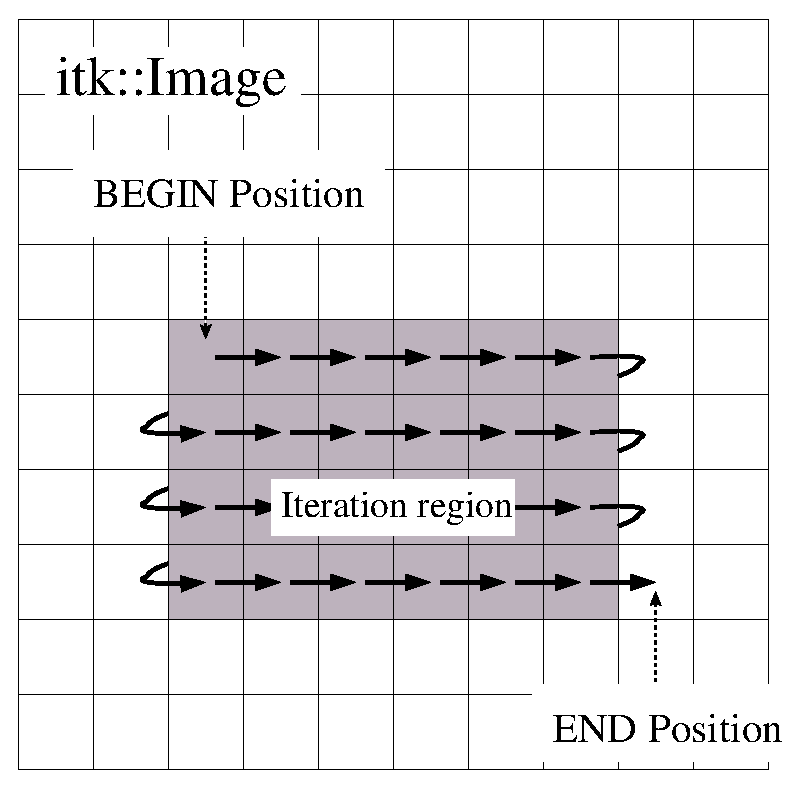
\includegraphics[width=0.4\textwidth]{IteratorFigure1.eps}
\itkcaption[ITK image iteration]{Normal path of an iterator through a
2D image.  The iteration region is shown in a darker shade.  An arrow denotes
a single iterator step, the result of one \code{++} operation.}
\protect\label{fig:WalkingIterator}
\end{figure}

In addition to sequential iteration through the image, some iterators may define
random access operators.  Unlike the increment operators, random access
operators may not be optimized for speed and require some knowledge of the
dimensionality of the image and the extent of the iteration region to use properly.

\begin{itemize}
\index{Iterators!operator+=()}
\item \textbf{\code{operator+=( OffsetType )}} Moves the iterator to the pixel
position at the current index plus specified \doxygen{Offset}.

\index{Iterators!operator-=()}
\item \textbf{\code{operator-=( OffsetType )}} Moves the iterator to
the pixel position at the current index minus specified Offset.

\index{Iterators!SetPosition()}
\item \textbf{\code{SetPosition( IndexType )}} Moves the iterator to the given
\doxygen{Index} position.
\end{itemize}

The \code{SetPosition()} method may be extremely slow for more complicated
iterator types. In general, it should only be used for setting a starting
iteration position, like you would use \code{GoToBegin()} or \code{GoToEnd()}.

Some iterators do not follow a predictable path through their
iteration regions and have no fixed beginning or ending pixel
locations.  A conditional iterator, for example, visits pixels only if
they have certain values or connectivities.  Random iterators,
increment and decrement to random locations and may even visit a given
pixel location more than once.

%Testing for location
An iterator can be queried to determine if it is at the end or the beginning of
its iteration region.

\begin{itemize}
\index{Iterators!IsAtEnd()}
\item \textbf{\code{bool IsAtEnd()}} True if the iterator points to \emph{one
position past} the end of the iteration region.

\index{Iterators!IsAtBegin()}
\item \textbf{\code{bool IsAtBegin()}} True if the iterator points to the first
position in the iteration region.  The method is typically used to test for the
end of reverse iteration.

\end{itemize}

An iterator can also report its current image index position.

\begin{itemize}
\index{Iterators!GetIndex()}
\item \textbf{\code{IndexType GetIndex()}} Returns the Index
of the image pixel that the iterator currently points to.
\end{itemize}

% A note on bounds checking
\index{Iterators!and bounds checking}
For efficiency, most ITK image iterators do not perform bounds checking.  It is
possible to move an iterator outside of its valid iteration region.
Dereferencing an out-of-bounds iterator will produce undefined results.

\subsection{Accessing Data}
\label{sec:AccessingData}
ITK image iterators define two basic methods for reading and writing pixel
values.

\begin{itemize}
\index{Iterators!Get()}
\item \textbf{\code{PixelType Get()}} Returns the value of the pixel at the
iterator position.

\index{Iterators!Set()}
\item \textbf{\code{void Set( PixelType )}} Sets the value of the pixel at the
iterator position.  Not defined for const versions of iterators.
\end{itemize}

% Describe efficiency due to inlining for all cases
The \code{Get()} and \code{Set()} methods are inlined and optimized
for speed so that their use is equivalent to dereferencing the image
buffer directly.  There are a few common cases, however, where using
\code{Get()} and \code{Set()} do incur a penalty. Consider the
following code, which fetches, modifies, and then writes a value back
to the same pixel location.

\small
\begin{minted}[baselinestretch=1,fontsize=\footnotesize,linenos=false,bgcolor=ltgray]{cpp}
  it.Set(it.Get() + 1);
\end{minted}
\normalsize

As written, this code requires one more memory dereference than is necessary.
Some iterators define a third data access method that avoids this penalty.

\begin{itemize}
\index{Iterators!Value()}
\item \textbf{\code{PixelType \& Value()}} Returns a reference to the pixel at
the iterator position.
\end{itemize}

The \code{Value()} method can be used as either an lval or an rval in an
expression.  It has all the properties of \code{operator*}.  The
\code{Value()} method makes it possible to rewrite our example code more
efficiently.

\small
\begin{minted}[baselinestretch=1,fontsize=\footnotesize,linenos=false,bgcolor=ltgray]{cpp}
  it.Value()++;
\end{minted}
\normalsize

Consider using the \code{Value()} method instead of \code{Get()} or
\code{Set()} when a call to \code{operator=} on a pixel is non-trivial, such as
when working with vector pixels, and operations are done in-place in the
image. The disadvantage of using \code{Value} is that it cannot support image
adapters (see Section~\ref{sec:ImageAdaptors} on
page~\pageref{sec:ImageAdaptors} for more information about image adaptors).

\subsection{Iteration Loops}
\label{sec:IterationExample}
% Now give a pseudo code example for putting all of this together.
Using the methods described in the previous sections, we can now write a simple
example to do pixel-wise operations on an image.  The following code calculates
the squares of all values in an input image and writes them to an output image.

\small
\begin{minted}[baselinestretch=1,fontsize=\footnotesize,linenos=false,bgcolor=ltgray]{cpp}
  ConstIteratorType in(inputImage, inputImage->GetRequestedRegion());
  IteratorType      out(outputImage, inputImage->GetRequestedRegion());

  for (in.GoToBegin(), out.GoToBegin(); !in.IsAtEnd(); ++in, ++out)
  {
    out.Set(in.Get() * in.Get());
  }
\end{minted}
\normalsize

\index{Iterators!and image regions}
Notice that both the input and output iterators are initialized over the same
region, the \code{RequestedRegion} of \code{inputImage}.  This is good
practice because it ensures that the output iterator walks exactly the same set
of pixel indices as the input iterator, but does not require that the output
and input be the same size. The only requirement is that the input image
must contain a region (a starting index and size) that matches the
\code{RequestedRegion} of the output image.

\index{reverse iteration}
Equivalent code can be written by iterating through the image in reverse.
The syntax is slightly more awkward because the \emph{end} of the
iteration region is not a valid position and we can only test whether the
iterator is strictly \emph{equal} to its beginning position.  It is often more
convenient to write reverse iteration in a \code{while} loop.

\small
\begin{minted}[baselinestretch=1,fontsize=\footnotesize,linenos=false,bgcolor=ltgray]{cpp}
  in.GoToEnd();
  out.GoToEnd();
  while (!in.IsAtBegin())
  {
    --in;
    --out;
    out.Set(in.Get() * in.Get());
  }
\end{minted}
\normalsize

%\begin{itemize}
%\item \textbf{\code{operator==}}
%\item \textbf{\code{operator<}}
%\item \textbf{\code{operator<=}}
%\item \textbf{\code{operator>}}
%\item \textbf{\code{operator>=}}
%\end{itemize}

%operator +=, -=, etc

% SetIndex()

% operator <, operator >, etc.

\index{Iterators!programming interface|)}
\section{Image Iterators}
\label{sec:ImageIterators}
%Introduction and overview
This section describes iterators that walk rectilinear image regions and
reference a single pixel at a time.  The \doxygen{ImageRegionIterator} is the
most basic ITK image iterator and the first choice for most applications. The
rest of the iterators in this section are specializations of
ImageRegionIterator that are designed make common image processing
tasks more efficient or easier to implement.

% Each of the iterators has a const and non-const version

\subsection{ImageRegionIterator}
\index{itk::ImageRegionIterator|(}
\label{sec:itkImageRegionIterator}
\input{ImageRegionIterator.tex}
\index{itk::ImageRegionIterator|)}

\subsection{ImageRegionIteratorWithIndex}
\label{sec:itkImageRegionIteratorWithIndex}
\index{itk::ImageRegionIteratorWithIndex|(}
\input{ImageRegionIteratorWithIndex.tex}
\index{itk::ImageRegionIteratorWithIndex|)}

\subsection{ImageLinearIteratorWithIndex}
\label{sec:itkImageLinearIteratorWithIndex}
\index{itk::ImageLinearIteratorWithIndex|(}
\input{ImageLinearIteratorWithIndex.tex}
\input{ImageLinearIteratorWithIndex2.tex}
\index{itk::ImageLinearIteratorWithIndex|)}

\subsection{ImageSliceIteratorWithIndex}
\label{sec:itkImageSliceIteratorWithIndex}
\index{itk::ImageSliceIteratorWithIndex|(}
\input{ImageSliceIteratorWithIndex.tex}
\index{itk::ImageSliceIteratorWithIndex|)}

\subsection{ImageRandomConstIteratorWithIndex}
\label{sec:itkImageRandomConstIteratorWithIndex}
\index{itk::Image\-Random\-Const\-Iterator\-With\-Index|(}
\input{ImageRandomConstIteratorWithIndex}
\index{itk::Image\-Random\-Const\-Iterator\-With\-Index|)}

%\section{Conditional Iterators}
%\index{Iterators!conditional|(}
%\label{sec:ConditionalIterators}
%This section describes iterators that walk only pixels in an image region whose
%values satisfy a specified condition.  The condition is usually based on some
%function of the image values, such as comparing to a threshold.  When the
%condition function returns \code{true} at a pixel location, the iterator
%includes that location in its path.  The biggest use of these iterators is for
%walking non-rectilinear regions of interest, such as might be defined by
%implicit geometric shape functions or connected component regions.

%./Common/itkConditionalConstIterator.h (BaseClass)
%./Common/itkConditionalIterator.h (BaseClass)
%./Common/itkFloodFilledFunctionConditionalConstIterator.h (BaseClass)
%./Common/itkFloodFilledFunctionConditionalIterator.h (BaseClass)

%[ here are all classes where these filters are used:
% ./BasicFilters/itkConfidenceConnectedImageFilter.hxx (ImageFunction)
% ./BasicFilters/itkConnectedThresholdImageFilter.hxx (ImageFunction)
% ./BasicFilters/itkIsolatedConnectedImageFilter.hxx (ImageFunction)
% ./BasicFilters/itkNeighborhoodConnectedImageFilter.hxx (ImageFunction)
%
% ./Common/itkBinaryBallStructuringElement.hxx (SpatialFunction)
% ./Common/itkBloxCoreAtomImage.hxx (SpatialFunction)
% ./BasicFilters/itkBloxBoundaryPointToCoreAtomImageFilter.hxx (SpatialFunction)
% ./BasicFilters/itkBloxBoundaryPointImageToBloxBoundaryProfileImageFilter.hxx (SpatialFunction)
%]

%\subsection{itk::FloodFilledImageFunctionConditionalIterator}
%\label{itk::FloodFilledImageFunctionConditionalIterator}
%\index{itk::FloodFilledImageFunctionConditionalIterator|(}
%./Common/itkFloodFilledImageFunctionConditionalConstIterator.h
%./Common/itkFloodFilledImageFunctionConditionalIterator.h
%\index{itk::FloodFilledImageFunctionConditionalIterator|)}

%\subsection{itk::FloodFilledSpatialFunctionConditionalIterator}
%\label{itk::FloodFilledSpatialFunctionConditionalIterator}
%\index{itk::FloodFilledSpatialFunctionConditionalIterator|(}
%./Common/itkFloodFilledSpatialFunctionConditionalConstIterator.h
%./Common/itkFloodFilledSpatialFunctionConditionalIterator.h
%\index{itk::FloodFilledImageFunctionConditionalIterator|)}
%\index{Iterators!conditional|)}

\section{Neighborhood Iterators}
\label{sec:NeighborhoodIterators}
\index{Iterators!neighborhood|(}
In ITK, a pixel neighborhood is loosely defined as a small set of pixels that
are locally adjacent to one another in an image.  The size and shape
of a neighborhood, as well the connectivity among pixels in a neighborhood,
may vary with the application.

Many image processing algorithms are neighborhood-based, that is, the result at
a pixel $i$ is computed from the values of pixels in the ND neighborhood of
$i$. Consider finite difference operations in 2D.  A derivative at pixel index
$i = (j, k)$, for example, is taken as a weighted difference of the values
at $(j+1, k)$ and $(j-1, k)$. Other common examples of neighborhood operations
include convolution filtering and image morphology.

This section describes a class of ITK image iterators that are designed for
working with pixel neighborhoods. An ITK neighborhood iterator walks an image
region just like a normal image iterator, but instead of only referencing a
single pixel at each step, it simultaneously points to the entire ND
neighborhood of pixels.  Extensions to the standard iterator interface provide
read and write access to all neighborhood pixels and information
such as the size, extent, and location of the neighborhood.

Neighborhood iterators use the same operators defined in
Section~\ref{sec:IteratorsInterface} and the same code constructs as normal
iterators for looping through an
image. Figure~\ref{fig:NeighborhoodIteratorFig1} shows a neighborhood iterator
moving through an iteration region.  This iterator defines a $3x3$ neighborhood
around each pixel that it visits. The \emph{center} of the neighborhood
iterator is always positioned over its current index and all other neighborhood
pixel indices are referenced as offsets from the center index.  The pixel
under the center of the neighborhood iterator and all pixels under the shaded
area, or \emph{extent}, of the iterator can be dereferenced.

\begin{figure}
\centering
\includegraphics[width=0.6\textwidth]{NeighborhoodIteratorFig1.eps}
\itkcaption[Neighborhood iterator]{Path of a $3x3$ neighborhood
iterator through a 2D image region.  The extent of the neighborhood is
indicated by the hashing around the iterator position. Pixels that lie within
this extent are accessible through the iterator.  An arrow denotes a single
iterator step, the result of one \code{++} operation.}
\protect\label{fig:NeighborhoodIteratorFig1}
\end{figure}

\index{Neighborhood iterators!construction of}
\index{Neighborhood iterators!radius of}

In addition to the standard image pointer and iteration region
(Section~\ref{sec:IteratorsInterface}), neighborhood iterator constructors
require an argument that specifies the extent of the neighborhood to cover.
Neighborhood extent is symmetric across its center in each
axis and is given as an array of $N$ distances that are collectively called the
\emph{radius}. Each element $d$ of the radius, where $0 < d < N$ and
$N$ is the dimensionality of the neighborhood, gives the extent of the
neighborhood in pixels for dimension $N$.  The length of each face of the
resulting ND hypercube is $2d + 1$ pixels, a distance of $d$ on either side of
the single pixel at the neighbor center.
Figure~{\ref{fig:NeighborhoodIteratorFig2} shows the relationship between the
radius of the iterator and the size of the neighborhood for a variety of 2D
iterator shapes.

The radius of the neighborhood iterator is queried after construction
by calling the \code{GetRadius()} method.  Some other methods provide
some useful information about the iterator and its underlying image.

\begin{figure}
\centering
\includegraphics[width=0.9\textwidth]{NeighborhoodIteratorFig2.eps}
\itkcaption[Some possible neighborhood iterator shapes]{Several possible 2D
neighborhood iterator shapes are shown along with their radii and sizes.  A
neighborhood pixel can be dereferenced by its integer index (top) or its
offset from the center (bottom).  The center pixel of each iterator is
shaded.}
\protect\label{fig:NeighborhoodIteratorFig2}
\end{figure}

\begin{itemize}

\index{NeighborhoodIterator!GetRadius()}
\item \textbf{\code{SizeType GetRadius()}} Returns the ND radius of the
neighborhood as an \doxygen{Size}.

\index{NeighborhoodIterator!GetImagePointer()}
\item \textbf{\code{const ImageType *GetImagePointer()}} Returns the pointer to
the image referenced by the iterator.

\index{NeighborhoodIterator!Size()}
\item \textbf{\code{unsigned long Size()}} Returns the size in number of
pixels of the neighborhood.

\end{itemize}

The neighborhood iterator interface extends the normal ITK iterator interface
for setting and getting pixel values.  One way to dereference pixels is to
think of the neighborhood as a linear array where each pixel has a unique
integer index. The index of a pixel in the array is determined by incrementing
from the upper-left-forward corner of the neighborhood along the fastest
increasing image dimension: first column, then row, then slice, and so on.  In
Figure~\ref{fig:NeighborhoodIteratorFig2}, the unique integer index is shown
at the top of each pixel.  The center pixel is always at position $n/2$, where
$n$ is the size of the array.

\begin{itemize}

\index{NeighborhoodIterator!GetPixel()}
\item \textbf{\code{PixelType GetPixel(const unsigned int i)}} Returns the
value of the pixel at neighborhood position \code{i}.

\index{NeighborhoodIterator!SetPixel()}
\item \textbf{\code{void SetPixel(const unsigned int i, PixelType p)}}
Sets the value of the pixel at position \code{i} to \code{p}.

\end{itemize}

Another way to think about a pixel location in a neighborhood is as an
ND offset from the neighborhood center.  The upper-left-forward corner
of a $3x3x3$ neighborhood, for example, can be described by offset
$(-1, -1, -1)$.  The bottom-right-back corner of the same neighborhood
is at offset $(1, 1, 1)$.  In
Figure~\ref{fig:NeighborhoodIteratorFig2}, the offset from center is
shown at the bottom of each neighborhood pixel.

\begin{itemize}

\index{NeighborhoodIterator!GetPixel()}
\item \textbf{\code{PixelType GetPixel(const OffsetType \&o)}} Get the value of
the pixel at the position offset \code{o} from the neighborhood center.

\index{NeighborhoodIterator!SetPixel()}
\item \textbf{\code{void SetPixel(const OffsetType \&o, PixelType p)}} Set
the value at the position offset \code{o} from the neighborhood center to
the value \code{p}.

\end{itemize}

The neighborhood iterators also provide a shorthand for setting and getting the
value at the center of the neighborhood.

\index{NeighborhoodIterators!}
\begin{itemize}

\index{NeighborhoodIterator!GetCenterPixel()}
\item \textbf{\code{PixelType GetCenterPixel()}} Gets the value at the center
of the neighborhood.

\index{NeighborhoodIterator!SetCenterPixel()}
\item \textbf{\code{void SetCenterPixel(PixelType p)}} Sets the value at the
center of the neighborhood to the value \code{p}

\end{itemize}

There is another shorthand for setting and getting values for pixels that
lie some integer distance from the neighborhood center along one of the image
axes.

\index{NeighborhoodIterators!}
\begin{itemize}

\index{NeighborhoodIterator!GetNext()}
\item \textbf{\code{PixelType GetNext(unsigned int d)}} Get the value
immediately adjacent to the neighborhood center in the positive direction along
the \code{d} axis.

\index{NeighborhoodIterator!SetNext()}
\item \textbf{\code{void SetNext(unsigned int d, PixelType p)}} Set the value
immediately adjacent to the neighborhood center in the positive direction along
the \code{d} axis to the value \code{p}.

\index{NeighborhoodIterator!GetPrevious()}
\item \textbf{\code{PixelType GetPrevious(unsigned int d)}} Get the value
immediately adjacent to the neighborhood center in the negative direction along
the \code{d} axis.

\index{NeighborhoodIterator!SetPrevious()}
\item \textbf{\code{void SetPrevious(unsigned int d, PixelType p)}}
Set the value immediately adjacent to the neighborhood center in the
negative direction along the \code{d} axis to the value \code{p}.

\item \textbf{\code{PixelType GetNext(unsigned int d, unsigned int
s)}} Get the value of the pixel located \code{s} pixels from the
neighborhood center in the positive direction along the \code{d} axis.

\item \textbf{\code{void SetNext(unsigned int d, unsigned int s, PixelType p)}}
Set the value of the pixel located \code{s} pixels from the neighborhood center
in the positive direction along the \code{d} axis to value \code{p}.

\item \textbf{\code{PixelType GetPrevious(unsigned int d, unsigned int
s)}} Get the value of the pixel located \code{s} pixels from the
neighborhood center in the positive direction along the \code{d} axis.

\item \textbf{\code{void SetPrevious(unsigned int d, unsigned int s,
PixelType p)}} Set the value of the pixel located \code{s} pixels from
the neighborhood center in the positive direction along the \code{d}
axis to value \code{p}.

\end{itemize}

It is also possible to extract or set all of the neighborhood values
from an iterator at once using a regular ITK neighborhood object.
This may be useful in algorithms that perform a particularly large
number of calculations in the neighborhood and would otherwise require
multiple dereferences of the same pixels.

\begin{itemize}

\index{NeighborhoodIterator!GetNeighborhood()}
\index{NeighborhoodIterator!SetNeighborhood()}
\item \textbf{\code{NeighborhoodType GetNeighborhood()}} Return a
\doxygen{Neighborhood} of the same size and shape as the neighborhood
iterator and contains all of the values at the iterator position.

\item \textbf{\code{void SetNeighborhood(NeighborhoodType \&N)}} Set all
of the values in the neighborhood at the iterator position to those contained
in Neighborhood \code{N}, which must be the same size and shape as the
iterator.

\end{itemize}

Several methods are defined to provide information about the neighborhood.

\index{NeighborhoodIterators!}
\begin{itemize}

\index{NeighborhoodIterator!GetIndex()}
\item \textbf{\code{IndexType GetIndex()}} Return the image
index of the center pixel of the neighborhood iterator.

\item \textbf{\code{IndexType GetIndex(OffsetType o)}} Return the
image index of the pixel at offset \code{o} from the neighborhood
center.

\item \textbf{\code{IndexType GetIndex(unsigned int i)}} Return the
image index of the pixel at array position \code{i}.

\index{NeighborhoodIterator!GetOffset()}
\item \textbf{\code{OffsetType GetOffset(unsigned int i)}}  Return the offset
from the neighborhood center of the pixel at array position \code{i}.

\index{NeighborhoodIterator!GetNeighborhoodIndex()}
\item \textbf{\code{unsigned long GetNeighborhoodIndex(OffsetType o)}}
Return the array position of the pixel at offset \code{o} from the
neighborhood center.

\index{NeighborhoodIterator!GetSlice()}
\item \textbf{\code{std::slice GetSlice(unsigned int n)}} Return a
\code{std::slice} through the iterator neighborhood along axis \code{n}.

\end{itemize}

\index{Neighborhood iterators!boundary conditions}
\index{Neighborhood iterators!bounds checking}
A neighborhood-based calculation in a neighborhood close to an image
boundary may require data that falls outside the boundary.  The
iterator in Figure~\ref{fig:NeighborhoodIteratorFig1}, for example, is
centered on a boundary pixel such that three of its neighbors actually
do not exist in the image.  When the extent of a neighborhood falls
outside the image, pixel values for missing neighbors are supplied
according to a rule, usually chosen to satisfy the numerical
requirements of the algorithm.  A rule for supplying out-of-bounds
values is called a \emph{boundary condition}.

ITK neighborhood iterators automatically detect out-of-bounds dereferences and
will return values according to boundary conditions.  The boundary condition
type is specified by the second, optional template parameter of the iterator.
By default, neighborhood iterators use a Neumann condition where the first
derivative across the boundary is zero.  The Neumann rule simply returns the
closest in-bounds pixel value to the requested out-of-bounds location.  Several
other common boundary conditions can be found in the ITK toolkit.  They include
a periodic condition that returns the pixel value from the opposite side of the
data set, and is useful when working with periodic data such as Fourier
transforms, and a constant value condition that returns a set value $v$ for all
out-of-bounds pixel dereferences.  The constant value condition is equivalent
to padding the image with value $v$.

Bounds checking is a computationally expensive operation because it occurs each
time the iterator is incremented.  To increase efficiency, a neighborhood
iterator automatically disables bounds checking when it detects that it is
not necessary.  A user may also explicitly disable or enable bounds checking.
Most neighborhood based algorithms can minimize the need for bounds checking
through clever definition of iteration regions.  These techniques are explored
in Section~\ref{sec:NeighborhoodExample3}.

\begin{itemize}

\index{NeighborhoodIterator!NeedToUseBoundaryConditionOn()}
\item \textbf{\code{void NeedToUseBoundaryConditionOn()}} Explicitly turn
bounds checking on.  This method should be used with caution because
unnecessarily enabling bounds checking may result in a significant performance
decrease. In general you should allow the iterator to automatically determine
this setting.

\index{NeighborhoodIterator!NeedToUseBoundaryConditionOff()}
\item \textbf{\code{void NeedToUseBoundaryConditionOff()}} Explicitly disable
bounds checking. This method should be used with caution because disabling
bounds checking when it is needed will result in out-of-bounds reads and
undefined results.

\index{NeighborhoodIterator!OverrideBoundaryCondition()}
\item \textbf{\code{void OverrideBoundaryCondition(BoundaryConditionType *b)}}
Overrides the templated boundary condition, using boundary condition
object \code{b} instead. Object \code{b} should not be deleted until
it has been released by the iterator.  This method can be used to
change iterator behavior at run-time.

\index{NeighborhoodIterator!ResetBoundaryCondition()}
\item \textbf{\code{void ResetBoundaryCondition()}} Discontinues the use of any
run-time specified boundary condition and returns to using the condition
specified in the template argument.

\index{NeighborhoodIterator!SetPixel()}
\item \textbf{\code{void SetPixel(unsigned int i, PixelType p, bool
status)}} Sets the value at neighborhood array position \code{i} to value
\code{p}.  If the position \code{i} is out-of-bounds, \code{status} is set to
\code{false}, otherwise \code{status} is set to \code{true}.
\end{itemize}

The following sections describe the two ITK neighborhood iterator classes,
\doxygen{NeighborhoodIterator} and \doxygen{ShapedNeighborhoodIterator}.
Each has a const and a non-const version.  The shaped iterator is a refinement
of the standard NeighborhoodIterator that supports an
arbitrarily-shaped (non-rectilinear) neighborhood.

\subsection{NeighborhoodIterator}
\label{sec:itkNeighborhoodIterator}

\index{NeighborhoodIterator!examples}
\index{Neighborhood iterators!examples}
The standard neighborhood iterator class in ITK is the
\doxygen{NeighborhoodIterator}.  Together with its \code{const} version,
\doxygen{ConstNeighborhoodIterator}, it implements the complete API
described above.  This section provides several examples to illustrate the use
of NeighborhoodIterator.

\index{edge detection}
\index{Sobel operator}
\subsubsection{Basic neighborhood techniques: edge detection}
\label{sec:NeighborhoodExample1}
\input{NeighborhoodIterators1.tex}

\index{convolution filtering}
\index{Sobel operator}
\subsubsection{Convolution filtering: Sobel operator}
\label{sec:NeighborhoodExample2}
\input{NeighborhoodIterators2.tex}

\subsubsection{Optimizing iteration speed}
\label{sec:NeighborhoodExample3}
\input{NeighborhoodIterators3.tex}

\index{Gaussian blurring}
\subsubsection{Separable convolution: Gaussian filtering}
\label{sec:NeighborhoodExample4}
\input{NeighborhoodIterators4.tex}

\subsubsection{Slicing the neighborhood}
\label{sec:NeighborhoodExample5}
\input{NeighborhoodIterators5.tex}

\subsubsection{Random access iteration}
\label{sec:NeighborhoodExample6}
\input{NeighborhoodIterators6.tex}

%./Common/itkConstNeighborhoodIterator.h
%./Common/itkNeighborhoodIterator.h

% Example1: Edge detection using ``hand-coded'' Sobel operator
% Example2: Sobel edge detection using convolution filtering and Sobel operator
% Example3: Improving boundary condition efficiency
% Example4: gaussian filtering, separable convolution
% Example5: Slicing the neighborhood: gaussian filtering, separable convolution
% Example6: Advanced Neighborhood Techniques: local minima, local maxima

\subsection{ShapedNeighborhoodIterator}
\label{sec:itkShapedNeighborhoodIterator}
\index{ShapedNeighborhoodIterator}
\index{Neighborhood iterators!shaped}
\index{Neighborhood iterators!as stencils}
This section describes a variation on the neighborhood iterator called a
\emph{shaped} neighborhood iterator.  A shaped neighborhood is defined like
a bit mask, or \emph{stencil}, with different offsets in the rectilinear
neighborhood of the normal neighborhood iterator turned off or on to create a
pattern.  Inactive positions (those not in the stencil) are not updated during
iteration and their values cannot be read or written.  The shaped iterator is
implemented in the class \doxygen{ShapedNeighborhoodIterator}, which is a
subclass of
\doxygen{NeighborhoodIterator}.  A const version,
\doxygen{ConstShapedNeighborhoodIterator}, is also available.

\index{Neighborhood iterators!active neighbors}
\index{Neighborhood iterators!inactive neighbors}
Like a regular neighborhood iterator, a shaped neighborhood iterator must be
initialized with an ND radius object, but the radius of the neighborhood of a
shaped iterator only defines the set of \emph{possible} neighbors.  Any number
of possible neighbors can then be activated or deactivated.  The shaped
neighborhood iterator defines an API for activating neighbors.  When a neighbor
location, defined relative to the center of the neighborhood, is activated, it
is placed on the \emph{active list} and is then part of the stencil.  An
iterator can be ``reshaped'' at any time by adding or removing offsets from the
active list.

\begin{itemize}

\index{ShapedNeighborhoodIterator!ActivateOffset()}
\item \textbf{\code{void ActivateOffset(OffsetType \&o)}} Include the offset
\code{o} in the stencil of active neighborhood positions.  Offsets are relative
to the neighborhood center.

\index{ShapedNeighborhoodIterator!DeactivateOffset()}
\item \textbf{\code{void DeactivateOffset(OffsetType \&o)}} Remove the offset
\code{o} from the stencil of active neighborhood positions.  Offsets are
relative to the neighborhood center.

\index{ShapedNeighborhoodIterator!ClearActiveList()}
\item \textbf{\code{void ClearActiveList()}} Deactivate all positions in the
iterator stencil by clearing the active list.

\index{ShapedNeighborhoodIterator!GetActiveIndexListSize()}
\item \textbf{\code{unsigned int GetActiveIndexListSize()}} Return the number
of pixel locations that are currently active in the shaped iterator stencil.

\end{itemize}

Because the neighborhood is less rigidly defined in the shaped iterator, the
set of pixel access methods is restricted.  Only the \code{GetPixel()} and
\code{SetPixel()} methods are available, and calling these methods on an
inactive neighborhood offset will return undefined results.

For the common case of traversing all pixel offsets in a neighborhood, the
shaped iterator class provides an iterator through the active offsets in its
stencil.   This \emph{stencil iterator} can be incremented or decremented and
defines \code{Get()} and \code{Set()} for reading and writing the values in the
neighborhood.

\begin{itemize}
\index{ShapedNeighborhoodIterator!Iterator::Begin()}
\item \textbf{\code{ShapedNeighborhoodIterator::Iterator Begin()}} Return a
const or non-const iterator through the shaped iterator stencil that points to
the first valid location in the stencil.

\index{ShapedNeighborhoodIterator!Iterator::End()}
\item \textbf{\code{ShapedNeighborhoodIterator::Iterator End()}} Return a
const or non-const iterator through the shaped iterator stencil that points
\emph{one position past} the last valid location in the stencil.
\end{itemize}

The functionality and interface of the shaped neighborhood iterator is best
described by example.  We will use the ShapedNeighborhoodIterator to
implement some binary image morphology algorithms (see \cite{Gonzalez1993},
\cite{Castleman1996}, et al.).  The examples that follow implement erosion and
dilation.

\index{ShapedNeighborhoodIterator!examples of}
\subsubsection{Shaped neighborhoods: morphological operations}
\label{sec:ShapedNeighborhoodExample}
\input{ShapedNeighborhoodIterators1.tex}
\input{ShapedNeighborhoodIterators2.tex}

%./Common/itkConstShapedNeighborhoodIterator.h
%./Common/itkShapedNeighborhoodIterator.h

\index{Iterators!neighborhood|)}

% ADD A SECTION WITH TIPS, SUGGESTIONS ON USING ITERATORS?  EXTENDING ITERATORS?
% USING ITERATORS FOR MULTITHREADING EXAMPLE?
\index{Iterators!image|)}

\input{Architecture/ImageAdaptors.tex}


\part{Development Guidelines}

\chapter{How To Write A Filter}
\label{chapter:WriteAFilter}

This purpose of this chapter is help developers create their own
filter (process object).  This chapter is divided into four major
parts. An initial definition of terms is followed by an overview of
the filter creation process. Next, data streaming is discussed. The
way data is streamed in ITK must be understood in order to write
correct filters. Finally, a section on multi-threading describes what
you must do in order to take advantage of shared memory parallel
processing.

\section{Terminology}
\label{sec:Terminology}

The following is some basic terminology for the discussion that follows.
Chapter \ref{chapter:SystemOverview} provides additional background
information.

\begin{itemize}
        \item The \textbf{data processing pipeline} is a directed graph of
        \textbf{process} and \textbf{data objects}. The pipeline inputs,
        operators on, and outputs data.
        \index{data processing pipeline}
        \index{process object}
        \index{data object}

        \item A \textbf{filter}, or \textbf{process object}, has one or more
        inputs, and one or more outputs.
        \index{filter}

        \item A \textbf{source}, or source process object, initiates the data
        processing pipeline, and has one or more outputs.
        \index{source}

        \item A \textbf{mapper}, or mapper process object, terminates the
        data processing pipeline. The mapper has one or more outputs, and may
        write data to disk, interface with a display system, or interface to
        any other system.
        \index{mapper}

        \item A \textbf{data object} represents and provides access to
        data. In ITK, the data object (ITK class \doxygen{DataObject}) is
        typically of type \doxygen{Image} or \doxygen{Mesh}.
        \index{data object}

        \item A \textbf{region} (ITK class \doxygen{Region}) represents a
        piece, or subset of the entire data set.
        \index{region}

        \item An \textbf{image region} (ITK class \doxygen{ImageRegion})
        represents a structured portion of data. ImageRegion is implemented
        using the \doxygen{Index} and \doxygen{Size} classes
        \index{image region}

        \item A \textbf{mesh region} (ITK class \doxygen{MeshRegion})
        represents an unstructured portion of data.
        \index{mesh region}

        \item The \textbf{LargestPossibleRegion} is the theoretical single,
        largest piece (region) that could represent the entire dataset. The
        LargestPossibleRegion is used in the system as the measure of the
        largest possible data size.
        \index{LargestPossibleRegion}

        \item The \textbf{BufferedRegion} is a contiguous block of memory
        that is less than or equal to in size to the
        LargestPossibleRegion. The buffered region is what has actually been
        allocated by a filter to hold its output.
        \index{BufferedRegion}

        \item The \textbf{RequestedRegion} is the piece of the dataset that a
        filter is required to produce. The RequestedRegion is less than or
        equal in size to the BufferedRegion. The RequestedRegion may differ
        in size from the BufferedRegion due to performance reasons. The
        RequestedRegion may be set by a user, or by an application that needs
        just a portion of the data.
        \index{RequestedRegion}

        \item The \textbf{modified time} (represented by ITK class
        \doxygen{TimeStamp}) is a monotonically increasing integer value that
        characterizes a point in time when an object was last modified.
        \index{modified time}

        \item \textbf{Downstream} is the direction of dataflow, from sources
        to mappers.
        \index{pipeline!downstream}

        \item \textbf{Upstream} is the opposite of downstream, from mappers
        to sources.
        \index{pipeline!upstream}

        \item The \textbf{pipeline modified time} for a particular data
        object is the maximum modified time of all upstream data objects and
        process objects.
        \index{pipeline!modified time}

        \item The term \textbf{information} refers to metadata that
        characterizes data. For example, index and dimensions are information
        characterizing an image region.
        \index{pipeline!information}
\end{itemize}

\section{Overview of Filter Creation}
\label{sec:OverviewFilterCreation}
\index{filter!overview of creation}

\begin{floatingfigure}[rlp]{7cm}
  \centering
  \includegraphics[width=6cm]{DataPipelineOneConnection.eps}
  \caption[Relationship between DataObjects and ProcessObjects]
{Relationship between DataObject and ProcessObject.
\label{fig:DataPipeLineOneConnection}}
\end{floatingfigure}


Filters are defined with respect to the type of data they input (if
any), and the type of data they output (if any). The key to writing a
ITK filter is to identify the number and types of input and
output. Having done so, there are often superclasses that simplify
this task via class derivation. For example, most filters in ITK take
a single image as input, and produce a single image on output. The
superclass \doxygen{ImageToImageFilter} is a convenience class that
provide most of the functionality needed for such a filter.

Some common base classes for new filters include:

\begin{itemize}

  \item \code{ImageToImageFilter}: the most common filter base for
    segmentation algorithms.  Takes an image and produces a new image, by
    default of the same dimensions.  Override
    \code{GenerateOutputInformation} to produce a different size.

  \item \code{UnaryFunctorImageFilter}: used when defining a filter that
  applies a function to an image.

  \item \code{BinaryFunctorImageFilter}: used when defining a filter that
  applies an operation to two images.

  \item \code{ImageFunction}: a functor that can be applied to an image,
  evaluating $f(x) $ at each point in the image.

  \item \code{MeshToMeshFilter}: a filter that transforms meshes, such as
  tessellation, polygon reduction, and so on.

  \item \code{LightObject}: abstract base for filters that don't fit well
  anywhere else in the class hierarchy.  Also useful for ``calculator''
  filters; i.e. a sink filter that takes an input and calculates a result
  which is retrieved using a \code{Get()} method.

\end{itemize}

Once the appropriate superclass is identified, the filter writer
implements the class defining the methods required by most all ITK
objects: \code{New()}, \code{PrintSelf()}, and protected constructor,
copy constructor, delete, and operator=, and so on. Also, don't forget
standard type aliases like \code{Self}, \code{Superclass}, \code{Pointer}, and
\code{ConstPointer}. Then the filter writer can focus on the most important
parts of the implementation: defining the API, data members, and other
implementation details of the algorithm. In particular, the filter writer
will have to implement either a \code{GenerateData()} (non-threaded) or
\code{ThreadedGenerateData()} and \code{DynamicThreadedGenerateData()} methods.
(See Section~\ref{sec:MultiThreading} for an overview of multi-threading in ITK.)

An important note: the GenerateData() method is required to allocate memory
for the output. The ThreadedGenerateData() method is not. In default
implementation (see \doxygen{ImageSource}, a superclass of
\doxygen{ImageToImageFilter})
\code{GenerateData()} allocates memory and then invokes
\code{DynamicThreadedGenerateData()} or \code{ThreadedGenerateData()}.

One of the most important decisions that the developer must make is whether
the filter can stream data; that is, process just a portion of the input to
produce a portion of the output. Often superclass behavior works well: if the
filter processes the input using single pixel access, then the default
behavior is adequate. If not, then the user may have to a) find a more
specialized superclass to derive from, or b) override one or more methods
that control how the filter operates during pipeline execution. The next
section describes these methods.



\section{Streaming Large Data}
\label{sec:StreamingLargeData}
\index{pipeline!streaming large data}

The data associated with multi-dimensional images is large and becoming larger.
This trend is due to advances in scanning resolution, as well as increases in
computing capability. Any practical segmentation and registration software
system must address this fact in order to be useful in application. ITK
addresses this problem via its data streaming facility.

In ITK, streaming is the process of dividing data into pieces, or regions,
and then processing this data through the data pipeline. Recall that the
pipeline consists of process objects that generate data objects, connected
into a pipeline topology. The input to a process object is a data object
(unless the process initiates the pipeline and then it is a source process
object). These data objects in turn are consumed by other process objects,
and so on, until a directed graph of data flow is constructed. Eventually the
pipeline is terminated by one or more mappers, that may write data to
storage, or interface with a graphics or other system. This is illustrated in
figures \ref{fig:DataPipeLineOneConnection} and \ref{fig:DataPipeLine}.

A significant benefit of this architecture is that the relatively complex
process of managing pipeline execution is designed into the system. This
means that keeping the pipeline up to date, executing only those portions of
the pipeline that have changed, multi-threading execution, managing memory
allocation, and streaming is all built into the architecture. However, these
features do introduce complexity into the system, the bulk of which is seen
by class developers. The purpose of this chapter is to describe the pipeline
execution process in detail, with a focus on data streaming.


\subsection{Overview of Pipeline Execution}
\label{sec:OverviewPipelineExecution}
\index{pipeline!overview of execution}

The pipeline execution process performs several important functions.

\begin{figure}
  \par\centering
  \resizebox{5in}{!}{ \includegraphics{DataPipeline.eps}}
  \itkcaption[The Data Pipeline]{The Data Pipeline}
  \label{fig:DataPipeLine}
  \par
\end{figure}

\begin{enumerate}
        \item It determines which filters, in a pipeline of filters, need to
        execute. This prevents redundant execution and minimizes overall
        execution time.

        \item It initializes the (filter's) output data objects, preparing
        them for new data.  In addition, it determines how much memory each
        filter must allocate for its output, and allocates it.

        \item The execution process determines how much data a filter must
        process in order to produce an output of sufficient size for
        downstream filters; it also takes into account any limits on memory
        or special filter requirements. Other factors include the size of
        data processing kernels, that affect how much data input data
        (extra padding) is required.

        \item It subdivides data into subpieces for multi-threading. (Note
        that the division of data into subpieces is exactly same problem as
        dividing data into pieces for streaming; hence multi-threading comes
        for free as part of the streaming architecture.)

        \item It may free (or release) output data if filters no longer need
        it to compute, and the user requests that data is to be
        released. (Note: a filter's output data object may be considered a
        ``cache''. If the cache is allowed to remain (\code{ReleaseDataFlagOff()})
        between pipeline execution, and the filter, or the input to the
        filter, never changes, then process objects downstream of the filter
        just reuse the filter's cache to re-execute.)
\end{enumerate}

To perform these functions, the execution process negotiates with the
filters that define the pipeline. Only each filter can know how much data is
required on input to produce a particular output. For example, a shrink
filter with a shrink factor of two requires an image twice as large (in terms
of its x-y dimensions) on input to produce a particular size output. An
image convolution filter would require extra input (boundary padding)
depending on the size of the convolution kernel. Some filters require the
entire input to produce an output (for example, a histogram), and have the
option of requesting the entire input. (In this case streaming does not work
unless the developer creates a filter that can request multiple pieces,
caching state between each piece to assemble the final output.)


\begin{figure}
  \par\centering
  \resizebox{5in}{!}{ \includegraphics{DataPipelineUpdate.eps}}
  \itkcaption[Sequence of the Data Pipeline updating mechanism]{Sequence of the
Data Pipeline updating mechanism}
  \label{fig:DataPipeLineUpdate}
  \par
\end{figure}


Ultimately the negotiation process is controlled by the request for data of a
particular size (i.e., region). It may be that the user asks to process a
region of interest within a large image, or that memory limitations result in
processing the data in several pieces. For example, an application may
compute the memory required by a pipeline, and then use
\doxygen{StreamingImageFilter} to break the data processing into several pieces.
The data request is propagated through the pipeline in the upstream
direction, and the negotiation process configures each filter to produce
output data of a particular size.

The secret to creating a streaming filter is to understand how this
negotiation process works, and how to override its default behavior by using
the appropriate virtual functions defined in \doxygen{ProcessObject}. The next
section describes the specifics of these methods, and when to override
them. Examples are provided along the way to illustrate concepts.


\subsection{Details of Pipeline Execution}
\label{sec:DetailsPipelineExecution}
\index{pipeline!execution details}

Typically pipeline execution is initiated when a process object
receives the \code{ProcessObject::Update()} method invocation. This
method is simply delegated to the output of the filter, invoking the
\code{DataObject::Update()} method. Note that this behavior is typical
of the interaction between ProcessObject and DataObject: a method
invoked on one is eventually delegated to the other. In this way the
data request from the pipeline is propagated upstream, initiating data
flow that returns downstream.

The \code{DataObject::Update()} method in turn invokes three other methods:

\begin{itemize}
        \item \code{DataObject::UpdateOutputInformation()}
        \item \code{DataObject::PropagateRequestedRegion()}
        \item \code{DataObject::UpdateOutputData()}
\end{itemize}

\subsubsection{UpdateOutputInformation()}
\label{sec:UpdateOutputInformation}
\index{pipeline!UpdateOutputInformation}

The \code{UpdateOutputInformation()} method first calls the
\code{VerifyPreconditions} to check that all required inputs
are set and all parameters are valid and consistent. This enables quick
failure of a filter when not configure correctly. The default
implementation checks that all required pipeline inputs are set.

Next the pipeline modified time is determined. The RequestedRegion is
set to process all the data, i.e., the LargestPossibleRegion, if
neither \code{UpdateLargestPossibleRegion} was called nor
RequestedRegion has not been set. The \code{UpdateOutputInformation()}
propagates upstream through the entire pipeline and terminates at the
sources.

After the upstream inputs have completed their
\code{UpdateOutputInformation} the metadata of inputs are
available. The \code{VerifyInputInformation} is then called. The
default implementation in \code{ImageToImageFilter} checks that all
input images occupy the same physical space. This may need to be
overridden if the filter does not require the image's voxels occupy the
same physical space.

During \code{UpdateOutputInformation()}, filters have a chance to override the
\code{ProcessObject::GenerateOutputInformation()} method
(\code{GenerateOutputInformation()} is invoked by
\code{UpdateOutputInformation()}). The default behavior is for the
\code{GenerateOutputInformation()} to copy the metadata describing the input
to the output (via \code{DataObject::CopyInformation()}). Remember, information
is metadata describing the output, such as the origin, spacing,
and LargestPossibleRegion (i.e., largest possible size) of an image.

A good example of this behavior is \doxygen{ShrinkImageFilter}. This filter
takes an input image and shrinks it by some integral value. The result is that
the spacing and LargestPossibleRegion of the output will be different to that
of the input. Thus, \code{GenerateOutputInformation()} is overloaded.

\subsubsection{PropagateRequestedRegion()}
\label{sec:PropagateRequestedRegion}
\index{pipeline!PropagateRequestedRegion}

The \code{PropagateRequestedRegion()} call propagates upstream to
satisfy a data request. In typical application this data request is usually the
LargestPossibleRegion, but if streaming is necessary, or the user is
interested in updating just a portion of the data, the RequestedRegion may be
any valid region within the LargestPossibleRegion.

The function of \code{PropagateRequestedRegion()} is, given a request
for data (the amount is specified by RequestedRegion), propagate
upstream configuring the filter's input and output process object's to
the correct size. Eventually, this means configuring the
BufferedRegion, that is the amount of data actually allocated.

The reason for the buffered region is this: the output of a filter may be
consumed by more than one downstream filter. If these consumers each request
different amounts of input (say due to kernel requirements or other padding
needs), then the upstream, generating filter produces the data to satisfy
both consumers, that may mean it produces more data than one of the
consumers needs.

The \code{ProcessObject::PropagateRequestedRegion()} method invokes
three methods that the filter developer may choose to overload.

\begin{itemize}
        \item \code{EnlargeOutputRequestedRegion(DataObject *output)} gives the
        (filter) subclass a chance to indicate that it will provide more data
        than required for the output. This can happen, for example, when a
        source can only produce the whole output (i.e., the
        LargestPossibleRegion).

        \item \code{GenerateOutputRequestedRegion(DataObject *output)} gives
        the subclass a chance to define how to set the requested regions for
        each of its outputs, given this output's requested region.  The default
        implementation is to make all the output requested regions the same.
        A subclass may need to override this method if each output is a
        different resolution. This method is only overridden if a filter has
        multiple outputs.

        \item \code{GenerateInputRequestedRegion()} gives the subclass a
        chance to
        request a larger requested region on the inputs. This is necessary
        when, for example, a filter requires more data at the ``internal''
        boundaries to produce the boundary values - due to kernel operations
        or other region boundary effects.
\end{itemize}

\doxygen{RGBGibbsPriorFilter} is an example of a filter that needs to
invoke \code{EnlargeOutputRequestedRegion()}. The designer of this
filter decided that the filter should operate on all the data. Note
that a subtle interplay between this method and
\code{GenerateInputRequestedRegion()} is occurring here. The default
behavior of \code{GenerateInputRequestedRegion()} (at least for
\doxygen{ImageToImageFilter}) is to set the input RequestedRegion to
the output's ReqestedRegion. Hence, by overriding the method
\code{EnlargeOutputRequestedRegion()} to set the output to the
LargestPossibleRegion, effectively sets the input to this filter to
the LargestPossibleRegion (and probably causing all upstream filters
to process their LargestPossibleRegion as well. This means that the
filter, and therefore the pipeline, does not stream. This could be
fixed by reimplementing the filter with the notion of streaming built
in to the algorithm.)

\doxygen{GradientMagnitudeImageFilter} is an example of a filter that needs to
invoke \code{GenerateInputRequestedRegion()}. It needs a larger input requested
region because a kernel is required to compute the gradient at a pixel. Hence
the input needs to be ``padded out'' so the filter has enough data to compute
the gradient at each output pixel.

\subsubsection{UpdateOutputData()}
\label{sec:UpdateOutputData}
\index{pipeline!UpdateOutputData}

\code{UpdateOutputData()} is the third and final method as a result of the
\code{Update()} method. The purpose of this method is to determine whether a
particular filter needs to execute in order to bring its output up to date. (A
filter executes when its \code{GenerateData()} method is invoked.) Filter
execution occurs when a) the filter is modified as a result of modifying an
instance variable; b) the input to the filter changes; c) the input data has
been released; or d) an invalid RequestedRegion was set previously and the
filter did not produce data. Filters execute in order in the downstream
direction.  Once a filter executes, all filters downstream of it must also
execute.

\code{DataObject::UpdateOutputData()} is delegated to the DataObject's source
(i.e., the ProcessObject that generated it) only if the DataObject needs to be
updated. A comparison of modified time, pipeline time, release data flag, and
valid requested region is made. If any one of these conditions indicate that
the data needs regeneration, then the source's
\code{ProcessObject::UpdateOutputData()} is invoked. These calls are made
recursively up the pipeline until a source filter object is encountered, or the
pipeline is determined to be up to date and valid. At this point, the recursion
unrolls, and the execution of the filter proceeds. (This means that the output
data is initialized, StartEvent is invoked, the filters \code{GenerateData()}
is called, EndEvent is invoked, and input data to this filter may be released,
if requested. In addition, this filter's InformationTime is updated to the
current time.)

The developer will never override \code{UpdateOutputData()}. The developer need
only write the \code{GenerateData()} method (non-threaded) or
\code{DynamicThreadedGenerateData()} method. A discussion on threading follows in the
next section.


\section{Threaded Filter Execution}
\label{sec:ThreadedFilterExecution}
\index{pipeline!ThreadedFilterExecution}

Filters that can process data in pieces can typically multi-process
using the data parallel, shared memory implementation built into the
pipeline execution process. To create a multi-threaded filter, simply
define and implement a \code{DynamicThreadedGenerateData()}.
For example, a \doxygen{ImageToImageFilter} would create the method:

\small
\begin{minted}[baselinestretch=1,fontsize=\footnotesize,linenos=false,bgcolor=ltgray]{cpp}
  void
  DynamicThreadedGenerateData(
    const OutputImageRegionType & outputRegionForThread) override;
\end{minted}
\normalsize

The key to threading is to generate output for the output region given as
the parameter. In ITK, this is simple to do
because an output iterator can be created using the region provided. Hence
the output can be iterated over, accessing the corresponding input pixels as
necessary to compute the value of the output pixel.

Multi-threading requires caution when performing I/O (including using
\code{cout} or \code{cerr}) or invoking events. A safe practice is to allow
only the invoking thread to perform I/O or generate events.
If more than one thread tries to write to the same place at the same time,
the program can behave badly, and possibly even deadlock or crash.

\code{DynamicThreadedGenerateData} signature allows number of pieces
(output regions) to be processed to be different, usually bigger than the
number of real threads executing the work. In turn, this allows load
balancing. The number of work units controls filter parallelism,
and the name `threads' is reserved for real threads as exposed by
\doxygen{MultiThreaderBase} and its descendants.



\section{Filter Conventions}

In order to fully participate in the ITK pipeline, filters are expected to
follow certain conventions, and provide certain interfaces.  This section
describes the minimum requirements for a filter to integrate into the ITK
framework.

A filter should define public types for the class itself (\code{Self}) and
its \code{Superclass}, and \code{const} and non-\code{const} smart pointers,
thus:

\begin{minted}[baselinestretch=1,fontsize=\footnotesize,linenos=false,bgcolor=ltgray]{cpp}
  using Self = ExampleImageFilter;
  using Superclass = ImageToImageFilter<TImage, TImage>;
  using Pointer = SmartPointer<Self>;
  using ConstPointer = SmartPointer<const Self>;
\end{minted}

The \code{Pointer} type is particularly useful, as it is a smart pointer
that will be used by all client code to hold a reference-counted
instantiation of the filter.

Once the above types have been defined, you can use the following
convenience macros, which permit your filter to participate in the object
factory mechanism, and to be created using the canonical \code{::New()}:

\begin{minted}[baselinestretch=1,fontsize=\footnotesize,linenos=false,bgcolor=ltgray]{cpp}
  /** Method for creation through the object factory. */
  itkNewMacro(Self);

  /** Run-time type information (and related methods). */
  itkTypeMacro(ExampleImageFilter, ImageToImageFilter);
\end{minted}

The default constructor should be \code{protected}, and provide sensible
defaults (usually zero) for all parameters. The copy constructor and
assignment operator should not implemented in order to prevent instantiating
the filter without the factory methods (above). They should be declared in the
\code{public} section using the \code{ITK\_DISALLOW\_COPY\_AND\_ASSIGN} macro
(see Section~\ref{sec:UsingStandardMacros} on page
\pageref{sec:UsingStandardMacros}).

Finally, the template implementation code (in the \code{.hxx} file) should
be included, bracketed by a test for manual instantiation, thus:

\begin{minted}[baselinestretch=1,fontsize=\footnotesize,linenos=false,bgcolor=ltgray]{cpp}
#ifndef ITK_MANUAL_INSTANTIATION
#  include "itkExampleFilter.hxx"
#endif
\end{minted}

\subsection{Optional}

A filter can be printed to an \code{std::ostream} (such as \code{std::cout})
by implementing the following method:

\begin{minted}[baselinestretch=1,fontsize=\footnotesize,linenos=false,bgcolor=ltgray]{cpp}
  void
  PrintSelf(std::ostream & os, Indent indent) const;
\end{minted}

\noindent and writing the name-value pairs of the filter parameters to the
supplied output stream.  This is particularly useful for debugging.

\subsection{Useful Macros}

Many convenience macros are provided by ITK, to simplify filter coding.
Some of these are described below:

\begin{description}
\item [itkStaticConstMacro] Declares a static variable of the given type,
  with the specified initial value.
\item [itkGetMacro] Defines an accessor method for the specified scalar data
  member.  The convention is for data members to have a prefix of
  \code{m\_}.
\item [itkSetMacro] Defines a mutator method for the specified scalar data
  member, of the supplied type.  This will automatically set the
  \code{Modified} flag, so the filter stage will be executed on the next
  \code{Update()}.
\item [itkBooleanMacro] Defines a pair of \code{OnFlag} and \code{OffFlag}
  methods for a boolean variable \code{m\_Flag}.
\item [itkGetConstObjectMacro, itkSetObjectMacro] Defines an accessor and mutator
  for an ITK object.  The Get form returns a smart pointer to the object.
\end{description}

Much more useful information can be learned from browsing the source in
\code{Code/Common/itkMacro.h} and for the \doxygen{Object} and
\doxygen{LightObject} classes.



%
% Section on how to write composite filters
%
\input{DevelopmentGuidelines/WriteACompositeFilter.tex}


%
% TODO: include useful tips from mailing list as flagged
%

\chapter{How To Create A Module}
\label{chapter:CreateAModule}
\index{module}

The Insight Toolkit is organized into logical units of coherent functionality called
modules. These modules are self-contained in a directory, whose components
are organized into subdirectories with standardized names. A module usually has
dependencies on other modules, which it declares. A module is defined with
CMake scripts that inform the build system of its contents and dependencies.

Modules are organized into:

\begin{itemize}
  \item The \textbf{top level} directory.

  \item The \textbf{include} directory.

  \item The \textbf{src} directory.

  \item The \textbf{test} directory.

  \item The \textbf{wrapping} directory.
\end{itemize}

This chapter describes how to create a new module. The following sections  are
organized by the different directory components of the module. The chapter
concludes with a section on how to add a third-party library dependency to a
module.

Note that the Insight Toolkit community has adopted a Coding Style guideline
for the sake of consistentcy and readability of the code. Such guideline is
described in Chapter \ref{ch:CodingStyleGuide}.

\section{Name and dependencies}
\label{sec:NameAndDependencies}
\index{module!top level}

The top level directory of a module is used to define a module's name and its
dependencies. Two files are required:

\begin{enumerate}
  \item \code{CMakeLists.txt}
  \item \code{itk-module.cmake}
\end{enumerate}

The information described in these files is used to populate \code{<ModuleName>.cmake}
files in the ITK module registry. The module registry is located
at \code{<ITK build directory>/lib/cmake/\ITKVERSIONMAJORMINOR/Modules/} in a
build tree or
\code{<CMAKE\_INSTALL\_PREFIX>/lib/cmake/\ITKVERSIONMAJORMINOR/Modules/}
in an install tree. These module files declare information about the module
and what is required to use it. This includes its module dependencies, C++ include
directories required to build against it, the libraries to link against, and CMake
code required to use it in a CMake configured project.


\subsection{CMakeLists.txt}

When CMake starts processing a module, it begins with the top level
\code{CMakeLists.txt} file. At a minimum, the \code{CMakeLists.txt} should
contain

\begin{minted}[baselinestretch=1,fontsize=\footnotesize,linenos=false,bgcolor=ltgray]{cmake}
cmake_minimum_required(VERSION 3.8.2)
project(MyModule)

set(MyModule_LIBRARIES MyModule)

if(NOT ITK_SOURCE_DIR)
  find_package(ITK REQUIRED)
  list(APPEND CMAKE_MODULE_PATH ${ITK_CMAKE_DIR})
  include(ITKModuleExternal)
else()
  itk_module_impl()
endif()
\end{minted}

where \code{MyModule} is the name of the module.

The CMake variable \code{<module-name>\_LIBRARIES} should be set to the names
of the libraries, if any, that clients of the module need to link. This will be
the same name as the library generated with the \code{add\_library} command in
a module's \code{src} directory, described in further detail in the Libraries
Section~\ref{sec:Libraries}.

The path \code{if(NOT ITK\_SOURCE\_DIR)} is used when developing a module outside of the
ITK source tree, i.e. an External module. An External module can be made
available to the community by adding it to \code{Modules/Remote/*.remote.cmake}
Remote module index in the ITK repository per Section ~\ref{sec:GitRepository}.

The CMake macro \code{itk\_module\_impl} is defined in the file
\code{CMake/ITKModuleMacros.cmake}. It will initiate processing of the
remainder of a module's CMake scripts. The script \code{ITKModuleExternal}
calls \code{itk\_module\_impl} internally.


\subsection{itk-module.cmake}

The \code{itk-module.cmake} is also a required CMake script at the top level
of a module, but this file is used to declare

\begin{enumerate}
  \item The module name.
  \item Dependencies on other modules.
  \item Modules properties.
  \item A description of the module.
\end{enumerate}

In this file, first set a CMake variable with the module's
description followed by a call to the \code{itk\_module} macro, which is
already defined by the time the script is read. For example,
\code{itk-module.cmake} for the \texttt{ITKCommon} module is

\begin{minted}[baselinestretch=1,fontsize=\footnotesize,linenos=false,bgcolor=ltgray]{cmake}
set(DOCUMENTATION "This module contains the central classes of the ITK
toolkit.  They include, basic data structures \(such as Points, Vectors,
Images, Regions\) the core of the process objects \(such as base
classes for image filters\) the pipeline infrastructure classes, the support
for multi-threading, and a collection of classes that isolate ITK from
platform specific features. It is anticipated that most other ITK modules will
depend on this one.")

itk_module(ITKCommon
  ENABLE_SHARED
  PRIVATE_DEPENDS
    ITKDoubleConversion
  COMPILE_DEPENDS
    ITKKWSys
    ITKVNLInstantiation
  TEST_DEPENDS
    ITKTestKernel
    ITKMesh
    ITKImageIntensity
    ITKIOImageBase
  DESCRIPTION
    "${DOCUMENTATION}"
)
\end{minted}

The description for the module should be escaped as a CMake string, and it
should be formatted with Doxygen markup. This description is added to ITK's
generated Doxygen documentation when the module is added to the Remote module
index. The description should describe the purpose and content of the module
and reference an Insight Journal article for further information.

A module name is the only required positional argument to the
\code{itk\_module} macro. Named options that take one or argument are:

\begin{description}
  \item[DEPENDS]          Modules that will be publicly linked to this module.
    The header's used are added to \code{include/*.\{h,hxx\}} files.
  \item[PRIVATE\_DEPENDS] Modules that will be privately linked to this
    module. The header's used are only added to \code{src/*.cxx} files.
  \item[COMPILE\_DEPENDS] Modules that are needed at compile time by this module.
    The header's used are added to \code{include/*\{h,hxx\}} files but there
    is not a library to link against.
  \item[TEST\_DEPENDS]    Modules that are needed by this modules testing executables.
    The header's used are added to \code{test/*.cxx} files.
  \item[DESCRIPTION]      Free text description of the module.
\end{description}

Public dependencies are added to the module's
\code{INTERFACE\_LINK\_LIBRARIES}, which is a list of transitive link
dependencies.  When this module is linked to by another target, the libraries
listed (and recursively, their link interface libraries) will be provided to
the target also. Private dependencies are linked to by this module, but not
added to \code{INTERFACE\_LINK\_LIBRARIES}.

Compile Dependencies are added to CMake's list of dependencies for the current
module, ensuring that they are built before the current module, but they will
not be linked either publicly or privately. They are only used to support the
building of the current module.

The following additional options take no arguments:

\begin{description}
  \item[EXCLUDE\_FROM\_DEFAULT] Exclude this module from collection of modules
    enabled with the \code{ITK\_BUILD\_DEFAULT\_MODULES} CMake option.
  \item[ENABLE\_SHARED]         Build this module as a shared library if the
    \code{BUILD\_SHARED\_LIBS} CMake option is set.
\end{description}

All External and Remote modules should set the \code{EXCLUDE\_FROM\_DEFAULT}
option.


\section{Headers}
\label{sec:Headers}
\index{module!include}

Headers for the module, both \code{*.h} declaration headers and \code{*.hxx}
template definition headers, should be added to the \code{include} directory.
No other explicit CMake configuration is required.

This path will automatically be added to the build include directory paths for
libraries (\ref{sec:Libraries}) and tests (\ref{sec:Tests}) in the module and when
another module declares this module as a dependency.

When a module is installed, headers are installed into a single
directory common to all ITK header files.

When \code{BUILD\_TESTING} is enabled, a header test is automatically
created. This test simply builds a simple executable that \texttt{\#include}s
all header files in the \code{include} directory. This ensures that all
included headers can be found, which tests the module's dependency
specification per Section~\ref{sec:NameAndDependencies}.


\section{Libraries}
\label{sec:Libraries}
\index{module!src}

Libraries generated by a module are created from source files with the
\code{.cxx} extension in a module's \code{src} directory. Some modules are
header-only, and they will not generate any libraries; in this case, the
\code{src} directory is omitted. When present, the \code{src} directory should
contain a \code{CMakeLists.txt} file that describes how to build the library.
A minimal \code{CMakeLists.txt} file is as follows.

\begin{minted}[baselinestretch=1,fontsize=\footnotesize,linenos=false,bgcolor=ltgray]{cmake}
set(AModuleName_SRCS
  itkFooClass.cxx
  itkBarClass.cxx
  )

itk_module_add_library(AModuleName ${AModuleName_SRCS})
\end{minted}

The \code{itk\_module\_add\_library} macro will create a library with the
given sources. The macro will also link the library to the
libraries defined by the module dependency
specification per Section~\ref{sec:NameAndDependencies}. Additionally, the
macro will set CMake target properties associated with the current module to
the given target.

If the \code{ENABLE\_SHARED} option is set on a
module, a shared library will be generated when
the CMake option \code{BUILD\_SHARED\_LIBS} is enabled.  A library symbol
export specification header is also generated for the module.  For a module
with the name \texttt{AModuleName}, the generated header will have the name
\texttt{AModuleNameExport.h}. Include the export header in the module source
headers, and add the export specification macro to the contained classes.  The
macro name in this case would be called \texttt{AModuleName\_EXPORT}. For
example, the file \texttt{itkFooClass.h} would contain

\begin{minted}[baselinestretch=1,fontsize=\footnotesize,linenos=false,bgcolor=ltgray]{cpp}
#include "AModuleNameExport.h"

namespace itk
{

class AModuleName_EXPORT FooClass
{
...
\end{minted}

Modules that do not build a library in their \texttt{src} directory or do not
have export specifications on their class declarations should not set
\code{ENABLE\_SHARED}.


\section{Tests}
\label{sec:Tests}
\index{module!test}

Regression tests for a module are placed in the \code{test} directory. This
directory will contain a \texttt{CMakeLists.txt} with the CMake configuration,
test sources, and optional \texttt{Input} and \texttt{Baseline} directories,
which contain test input and baseline image datasets, respectively. Placement
of the input and baseline image datasets within a given module directory is
preferred over placement in the general \texttt{Testing/Data} directory; this
ensures that a module's data is only downloaded when the module is enabled. An
exception to this rule may be widely used input datasets, such as the
\texttt{cthead1.png} image.

An example CMake configuration for a test directory is shown below.

\begin{minted}[baselinestretch=1,fontsize=\footnotesize,linenos=false,bgcolor=ltgray]{cmake}
itk_module_test()

set(ModuleTemplateTests
  itkMinimalStandardRandomVariateGeneratorTest.cxx
  itkLogNormalDistributionImageSourceTest.cxx
  )

CreateTestDriver(ModuleTemplate "${ModuleTemplate-Test_LIBRARIES}" "${ModuleTemplateTests}")

itk_add_test(NAME itkMinimalStandardRandomVariateGeneratorTest
  COMMAND ModuleTemplateTestDriver itkMinimalStandardRandomVariateGeneratorTest
  )

itk_add_test(NAME itkLogNormalDistributionImageSourceTest
  COMMAND ModuleTemplateTestDriver --without-threads
  --compare
    ${ITK_TEST_OUTPUT_DIR}/itkLogNormalDistributionImageSourceTestOutput.mha
    DATA{Baseline/itkLogNormalDistributionImageSourceTestOutput.mha}
  itkLogNormalDistributionImageSourceTest
    ${ITK_TEST_OUTPUT_DIR}/itkLogNormalDistributionImageSourceTestOutput.mha
  )
\end{minted}

The \texttt{CMakeLists.txt} file should start with a call to the
\code{itk\_module\_test} macro. Next, the test sources are listed. The naming
convention for unit test files is \texttt{itk<ClassName>Test.cxx}. Each test
file should be written like a command line executable, but the name of the
\texttt{main} function should be replaced with the name of the test. The
function should accept \code{int argc, char * argv[]} as arguments. To reduce
the time required for linking and to provide baseline comparison functionality,
all tests are linked to into a single test driver executable. To generate the
executable, call the \code{CreateTestDriver} macro.

Tests are defined with the \code{itk\_add\_test} macro. This is a wrapper
around the CMake \code{add\_test} command that will resolve content links in
the \code{DATA} macro. Testing data paths are given inside the \code{DATA}
macro. Content link files, stored in the source code directory, are replaced
by actual content files in the build directory when CMake downloads the
\code{ITKData} target at build time. A content link file has the same name as
its target, but a \texttt{.md5} extension is added, and the \texttt{.md5}
file's contents are only the MD5SUM hash of its target. Content links for data
files in a Git distributed version control repository prevent repository
bloat. To obtain content links, register an account with the \texttt{ITK}
community at \url{https://midas3.kitware.com} and request upload permissions
on the ITK mailing list. The content links may also be created locally: once
the actual file at issue has been placed in the corresponding directory, run
CMake configuration, and CMake provides the desired \texttt{.md5} extension
content link file.

When a test requires a new (or modified) input or baseline image dataset,
the corresponding content link files have to be provided as well. Image
datasets provided should be kept as small as possible. As a rule of thumb,
their size should be under 50~\textit{kB}.

Test commands should call the test driver executable, followed by options for
the test, followed by the test function name, followed by arguments that are
passed to the test. The test driver accepts options like \texttt{--compare}
(or \texttt{--compare-MD5} when using the MD5SUM hash) to compare output images
to baselines or options that modify tolerances on comparisons. An exhaustive
list of options is displayed in \texttt{itkTestDriverInclude.h}.

A few rules must be acknowledged to actually write a units test file
\texttt{itk<ClassName>Test.cxx} for a given ITK class:
\begin{enumerate}
\item All class methods must be exercised.
\item Test cases with values for member variables different from the default
ones should be provided. The usefulness of this rule is especially manifest
for boolean members, whose value usually determines whether a large portion
of code is exercised or not.
\item Test cases to reach the exception cases within the class should be
provided.
\item Regression tests must be included for methods returning a value.
\item When a test detects a failure condition it must return the
\code{EXIT\_FAILURE} value; if a test exits normally, it must return
the \code{EXIT\_SUCCESS} value.
\end{enumerate}

In any case, ITK provides with a number of classes and macros that ease the
process of writing tests and checking the expected results. The following is an
exhaustive list of such tools:
\begin{itemize}
\item \texttt{itkTestingMacros.h}: it contains a number of macros that allow
testing of basic object properties:
\begin{itemize}
\item \code{EXERCISE\_BASIC\_OBJECT\_METHODS()}: verifies whether the class and
superclass names provided match the RTTI, and exercises the \code{PrintSelf()}
method. Since the \code{PrintSelf()} method prints all class member variables,
this macro, when exercised, can identify uninitialized member variables.
\item \code{TEST\_SET\_GET\_VALUE()}: once a member variable value has been set
using the corresponding Set macro, this macro verifies that the value provided
to the \code{Set()} method was effectively assigned to the member variable
by comparing it to the value returned by the \code{Get()} value.
\item \code{TEST\_SET\_GET\_BOOLEAN()}: exercises the \code{Set()/Get()},
and \code{On()/Off()} methods of class applied to a boolean member variable.
\end{itemize}
\item \code{TRY\_EXPECT\_NO\_EXCEPTION()}: exercises a method which is expected to
return with no errors. It is only required for methods that are known to throw
exceptions, such as I/O operations, filter updates, etc.
\item \code{TRY\_EXPECT\_EXCEPTION()}: exercises a method in the hope of detecting
an exception. This macro allows a test to continue its execution when setting
test cases bound to hit a class' exception cases. It is only required for
methods that are known to throw exceptions, such as I/O operations, filter
updates, etc.
\item \code{itkMath.h}: contains a series of static methods used for basic
type comparison. Methods are available to perform fuzzy floating point equality
comparison, e.g. \code{itk::Math::FloatAlmostEquals()}, to handle expected
cross-platform differences.
\end{itemize}

A test may have some input arguments. When a test does not need any input
argument (e.g., it generates a synthetic input image), the \code{main}
argument names may either be omitted (\code{int itk<ClassName>Test( int,
char* [] )}), or the \code{itkNotUsed }macro can be used (\code{int
itk<ClassName>Test( int itkNotUsed( argc ), char *itkNotUsed( argv ) [] )}),
to avoid compiler warnings about unused variables.

The number of input arguments provided must be checked at the beginning of the
test. If a test requires a fixed number of input arguments, then the argument
number check should verify the exact number of arguments.

It is essential that a test is made quantitative, i.e., the methods' returned
values and the test's output must be compared to a known ground-truth. As
mentioned, ITK contains a series of methods to compare basic types. ITK also
provide a powerful regression tool for a test that checks the validity of a
process over an image, which is the most common case in ITK. To this end, the
test is expected to write its output to a file. The first time the test is run,
the output is expected to be manually placed within the test module's
\texttt{Baseline} folder. Hence, when CTest is executed, the distance between
the test's output and the expected output (i.e., the baseline) is computed. If
the distance is below a configurable tolerance, the regression test is marked as
a success.

\section{Wrapping}
\label{sec:ModuleWrapping}
\index{module!wrapping}

Wrapping for programming languages like Python can be added to a module
through a simple configuration in the module's \code{wrapping} directory.
While wrapping is almost entirely automatic, configuration is necessary
to add two pieces of information,

\begin{enumerate}
  \item The types with which to instantiate templated classes.
  \item Class dependencies which must be wrapped before a given class.
\end{enumerate}

When wrapping a class, dependencies, like the base class and other types used
in the wrapped class's interface, should also be wrapped. The wrapping system
will emit a warning when a base class or other required type is not already
wrapped to ensure proper wrapping coverage. Since module dependencies are
wrapped by the build system before the current module, class wrapping
build order is already correct module-wise. However, it may be required to
wrap classes within a module in a specific order; this order can be specified
in the \code{wrapping/CMakeLists.txt} file.

Many ITK classes are templated, which allows an algorithm to be written once
yet compiled into optimized binary code for numerous pixel types and
spatial dimensions. When wrapping these templated classes, the template
instantiations to wrap must be chosen at build time. The template
that should be used are configured in a module's \code{*.wrap} files.
Wrapping is configured by calling CMake macros defined in the
\code{ITK/Wrapping/TypedefMacros.cmake} file.


\subsection{CMakeLists.txt}

The \code{wrapping/CMakeLists.txt} file calls three macros, and
optionally set a variable, \code{WRAPPER\_SUBMODULE\_ORDER}. The following
example is from the ITKImageFilterBase module:

\begin{minted}[baselinestretch=1,fontsize=\footnotesize,linenos=false,bgcolor=ltgray]{cmake}
itk_wrap_module(ITKImageFilterBase)

set(WRAPPER_SUBMODULE_ORDER
  itkRecursiveSeparableImageFilter
  itkFlatStructuringElement
  itkKernelImageFilter
  itkMovingHistogramImageFilterBase
)
itk_auto_load_submodules()
itk_end_wrap_module()
\end{minted}

The \code{itk\_wrap\_module} macro takes the current module name as an argument. In
some cases, classes defined in the \code{*.wrap} files within a module may depend
each other. The \code{WRAPPER\_SUBMODULE\_ORDER} variable is used to declare
which submodules should be wrapped first and the order they should be
wrapped.


\subsection{Class wrap files}

Wrapping specification for classes is written in the module's \code{*.wrap}
CMake script files. These files call wrapping CMake macros, and they specify
which classes to wrap, whether smart pointer's should be wrapped for the the
class, and which template instantiations to wrap for a class.

Overall toolkit class template instantiations are parameterized by the CMake
build configuration variables shown in Table~\ref{tab:WrappingVariables}.
The wrapping configuration refers to these settings with the shorthand values
listed in the second column.


\begin{table}
\begin{center}
\begin{tabular}{| l | l |}
\hline
\textbf{CMake variable} & \textbf{Wrapping shorthand value} \\
\hline
\hline
\code{ITK\_WRAP\_IMAGE\_DIMS} & List of unsigned integers \\
\hline
\code{ITK\_WRAP\_VECTOR\_COMPONENTS} & List of unsigned integers \\
\hline
\code{ITK\_WRAP\_double} & \code{D} \\
\hline
\code{ITK\_WRAP\_float} & \code{F} \\
\hline
\code{ITK\_WRAP\_complex\_double} & \code{CD} \\
\hline
\code{ITK\_WRAP\_complex\_float} & \code{CF} \\
\hline
\code{ITK\_WRAP\_vector\_double} & \code{VD} \\
\hline
\code{ITK\_WRAP\_vector\_float} & \code{VF} \\
\hline
\code{ITK\_WRAP\_covariate\_vector\_double} & \code{CVD} \\
\hline
\code{ITK\_WRAP\_covariate\_vector\_float} & \code{CVF} \\
\hline
\code{ITK\_WRAP\_signed\_char} & \code{SC} \\
\hline
\code{ITK\_WRAP\_signed\_short} & \code{SS} \\
\hline
\code{ITK\_WRAP\_signed\_long} & \code{SL} \\
\hline
\code{ITK\_WRAP\_unsigned\_char} & \code{UC} \\
\hline
\code{ITK\_WRAP\_unsigned\_short} & \code{US} \\
\hline
\code{ITK\_WRAP\_unsigned\_long} & \code{UL} \\
\hline
\code{ITK\_WRAP\_rgb\_unsigned\_char} & \code{RGBUC} \\
\hline
\code{ITK\_WRAP\_rgb\_unsigned\_short} & \code{RGBUS} \\
\hline
\code{ITK\_WRAP\_rgba\_unsigned\_char} & \code{RGBAUC} \\
\hline
\code{ITK\_WRAP\_rgba\_unsigned\_short} & \code{RGBAUS} \\
\hline
\end{tabular}
\end{center}
\itkcaption[Wrapping Configuration Variables]{CMake wrapping type
  configuration variables and their shorthand value in the wrapping
configuration.}
\label{tab:WrappingVariables}
\end{table}

Class wrap files call sets of wrapping macros for the class to be wrapped. The
macros are often called in loops over the wrapping variables to instatiate the
desired types. The following example demonstates wrapping the
\doxygen{ImportImageFilter} class, taken from the
\code{ITK/Modules/Core/Common/wrapping/itkImportImageFilter.wrap} file.

\begin{minted}[baselinestretch=1,fontsize=\footnotesize,linenos=false,bgcolor=ltgray]{cmake}
itk_wrap_class("itk::ImportImageFilter" POINTER)

  foreach(d ${ITK_WRAP_IMAGE_DIMS})
    foreach(t ${WRAP_ITK_SCALAR})
      itk_wrap_template("${ITKM_${t}}${d}" "${ITKT_${t}},${d}")
    endforeach()
  endforeach()

itk_end_wrap_class()
\end{minted}


\subsubsection{Wrapping Variables}

Instantiations for classes are determined by looping over CMake lists that
collect sets of shorthand wrapping values, namely,

\begin{itemize}
  \item \code{ITK\_WRAP\_IMAGE\_DIMS}
  \item \code{ITK\_WRAP\_IMAGE\_DIMS\_INCREMENTED}
    \\
  \item \code{ITK\_WRAP\_IMAGE\_VECTOR\_COMPONENTS}
  \item \code{ITK\_WRAP\_IMAGE\_VECTOR\_COMPONENTS\_INCREMENTED}
    \\
  \item \code{WRAP\_ITK\_USIGN\_INT}
  \item \code{WRAP\_ITK\_SIGN\_INT}
  \item \code{WRAP\_ITK\_INT}
    \\
  \item \code{WRAP\_ITK\_REAL}
  \item \code{WRAP\_ITK\_COMPLEX\_REAL}
    \\
  \item \code{WRAP\_ITK\_SCALAR}
    \\
  \item \code{WRAP\_ITK\_VECTOR\_REAL}
  \item \code{WRAP\_ITK\_COV\_VECTOR\_REAL}
  \item \code{WRAP\_ITK\_VECTOR}
    \\
  \item \code{WRAP\_ITK\_RGB}
  \item \code{WRAP\_ITK\_RGBA}
  \item \code{WRAP\_ITK\_COLOR}
    \\
  \item \code{WRAP\_ITK\_ALL\_TYPES}
\end{itemize}

Templated classes are wrapped as typedefs for particular instantiations. The
typedefs are named with a name mangling scheme for the template parameter
types. The mangling of common types are stored in CMake variables listed in
Table~\ref{tab:WrappingManglingForPODs},
Table~\ref{tab:WrappingManglingOtherITKPixelTypes}, and
Table~\ref{tab:WrappingManglingITKBasicTypes}. Mangling variables start with the prefix
\code{ITKM\_} and their corresponding C++ type variables start with the
prefix \code{ITKT\_}.

\begin{table}
\begin{center}
\begin{tabular}{l | l | l |}
\hline
& \textbf{CMake Variable} & \textbf{Value} \\
\hline
\hline
\textbf{Mangling} & ITKM\_B & B \\ \hline
\textbf{C++ Type} & ITKT\_B & bool \\ \hline
\\ \hline
\textbf{Mangling} & ITKM\_UC & UC \\ \hline
\textbf{C++ Type} & ITKT\_UC & unsigned char \\ \hline
\\ \hline
\textbf{Mangling} & ITKM\_US & US \\ \hline
\textbf{C++ Type} & ITKT\_US & unsigned short \\ \hline
\\ \hline
\textbf{Mangling} & ITKM\_UI & UI \\ \hline
\textbf{C++ Type} & ITKT\_UI & unsigned integer \\ \hline
\\ \hline
\textbf{Mangling} & ITKM\_UL & UL \\ \hline
\textbf{C++ Type} & ITKT\_UL & unsigned long \\ \hline
\\ \hline
\textbf{Mangling} & ITKM\_SC & SC \\ \hline
\textbf{C++ Type} & ITKT\_SC & signed char \\ \hline
\\ \hline
\textbf{Mangling} & ITKM\_SS & SS \\ \hline
\textbf{C++ Type} & ITKT\_SS & signed short \\ \hline
\\ \hline
\textbf{Mangling} & ITKM\_SI & SI \\ \hline
\textbf{C++ Type} & ITKT\_SI & signed integer \\ \hline
\\ \hline
\textbf{Mangling} & ITKM\_UL & UL \\ \hline
\textbf{C++ Type} & ITKT\_UL & signed long \\ \hline
\\ \hline
\textbf{Mangling} & ITKM\_F & F \\ \hline
\textbf{C++ Type} & ITKT\_F & float \\ \hline
\\ \hline
\textbf{Mangling} & ITKM\_D & D \\ \hline
\textbf{C++ Type} & ITKT\_D & double \\ \hline
\end{tabular}
\end{center}
\itkcaption[Wrapping CMake Mangling Variables for PODs]{CMake wrapping mangling
  variables, their values, and the corresponding CMake C++ type variables and
their values for plain old datatypes (PODS).}
\label{tab:WrappingManglingForPODs}
\end{table}

\begin{table}
\begin{center}
  \small
  \begin{tabular}{l | p{0.3\textwidth} | p{0.5\textwidth} |}
\hline
& \textbf{CMake Variable} & \textbf{Value} \\
\hline
\hline
\textbf{Mangling} & ITKM\_C\$\{type\} & C\$\{type\} \\ \hline
\textbf{C++ Type} & ITKT\_C\$\{type\} & std::complex\textless \$\{type\} \textgreater\\ \hline
\\ \hline
\textbf{Mangling} & ITKM\_A\$\{type\} & A\$\{type\} \\ \hline
\textbf{C++ Type} & ITKT\_A\$\{type\} & itk::Array\textless \$\{type\} \textgreater\\ \hline
\\ \hline
\textbf{Mangling} & ITKM\_FA\$\{ITKM\_\$\{type\}\}\$\{dim\} & FA\$\{ITKM\_\$\{type\}\}\$\{dim\} \\ \hline
\textbf{C++ Type} & ITKT\_FA\$\{ITKM\_\$\{type\}\}\$\{dim\} & itk::FixedArray\textless \$\{ITKT\_\$\{type\}\}, \$\{dim\} \textgreater \\ \hline
\\ \hline
\textbf{Mangling} & ITKM\_RGB\$\{dim\} & RGB\$\{dim\} \\ \hline
\textbf{C++ Type} & ITKT\_RGB\$\{dim\} & itk::RGBPixel\textless \$\{dim\} \textgreater\\ \hline
\\ \hline
\textbf{Mangling} & ITKM\_RGBA\$\{dim\} & RGBA\$\{dim\} \\ \hline
\textbf{C++ Type} & ITKT\_RGBA\$\{dim\} & itk::RGBAPixel\textless \$\{dim\} \textgreater\\ \hline
\\ \hline
\textbf{Mangling} & ITKM\_V\$\{ITKM\_\$\{type\}\}\$\{dim\} & V\$\{ITKM\_\$\{type\}\}\$\{dim\} \\ \hline
\textbf{C++ Type} & ITKT\_V\$\{ITKM\_\$\{type\}\}\$\{dim\} & itk::Vector\textless \$\{ITKT\_\$\{type\}\}, \$\{dim\} \textgreater \\ \hline
\\ \hline
\textbf{Mangling} & ITKM\_CV\$\{ITKM\_\$\{type\}\}\$\{dim\} & CV\$\{ITKM\_\$\{type\}\}\$\{dim\} \\ \hline
\textbf{C++ Type} & ITKT\_CV\$\{ITKM\_\$\{type\}\}\$\{dim\} & itk::CovariantVector\textless \$\{ITKT\_\$\{type\}\}, \$\{dim\} \textgreater \\ \hline
\\ \hline
\textbf{Mangling} & ITKM\_VLV\$\{ITKM\_\$\{type\}\}\$\{dim\} & VLV\$\{ITKM\_\$\{type\}\}\$\{dim\} \\ \hline
\textbf{C++ Type} & ITKT\_VLV\$\{ITKM\_\$\{type\}\}\$\{dim\} & itk::VariableLengthVector\textless \$\{ITKT\_\$\{type\}\}, \$\{dim\} \textgreater \\ \hline
\\ \hline
\textbf{Mangling} & ITKM\_SSRT\$\{ITKM\_\$\{type\}\}\$\{dim\} & SSRT\$\{ITKM\_\$\{type\}\}\$\{dim\} \\ \hline
\textbf{C++ Type} & ITKT\_SSRT\$\{ITKM\_\$\{type\}\}\$\{dim\} & itk::SymmetricSecondRankTensor\textless \$\{ITKT\_\$\{type\}\}, \$\{dim\} \textgreater \\ \hline
\end{tabular}
\end{center}
\itkcaption[Wrapping CMake Mangling Variables for other ITK pixel types.]{CMake wrapping mangling
  variables, their values, and the corresponding CMake C++ type variables and
  their values for other ITK pixel types.}
\label{tab:WrappingManglingOtherITKPixelTypes}
\end{table}


\begin{table}
\begin{center}
  \small
  \begin{tabular}{l | p{0.3\textwidth} | p{0.5\textwidth} |}
\hline
& \textbf{CMake Variable} & \textbf{Value} \\
\hline
\hline
\textbf{Mangling} & ITKM\_O\$\{dim\} & O\$\{dim\} \\ \hline
\textbf{C++ Type} & ITKT\_O\$\{dim\} & itk::Offset\textless \$\{dim\} \textgreater\\ \hline
\\ \hline
\textbf{Mangling} & ITKM\_CI\$\{ITKM\_\$\{type\}\}\$\{dim\} & CI\$\{ITKM\_\$\{type\}\}\$\{dim\} \\ \hline
\textbf{C++ Type} & ITKT\_CI\$\{ITKM\_\$\{type\}\}\$\{dim\} & itk::ContinuousIndex\textless \$\{ITKT\_\$\{type\}\}, \$\{dim\} \textgreater \\ \hline
\\ \hline
\textbf{Mangling} & ITKM\_P\$\{ITKM\_\$\{type\}\}\$\{dim\} & P\$\{ITKM\_\$\{type\}\}\$\{dim\} \\ \hline
\textbf{C++ Type} & ITKT\_P\$\{ITKM\_\$\{type\}\}\$\{dim\} & itk::Point\textless \$\{ITKT\_\$\{type\}\}, \$\{dim\} \textgreater \\ \hline
\\ \hline
\textbf{Mangling} & ITKM\_I\$\{ITKM\_\$\{type\}\}\$\{dim\} & I\$\{ITKM\_\$\{type\}\}\$\{dim\} \\ \hline
\textbf{C++ Type} & ITKT\_I\$\{ITKM\_\$\{type\}\}\$\{dim\} & itk::Image\textless \$\{ITKT\_\$\{type\}\}, \$\{dim\} \textgreater \\ \hline
\\ \hline
\textbf{Mangling} & ITKM\_VI\$\{ITKM\_\$\{type\}\}\$\{dim\} & VI\$\{ITKM\_\$\{type\}\}\$\{dim\} \\ \hline
\textbf{C++ Type} & ITKT\_VI\$\{ITKM\_\$\{type\}\}\$\{dim\} & itk::VectorImage\textless \$\{ITKT\_\$\{type\}\}, \$\{dim\} \textgreater \\ \hline
\\ \hline
\textbf{Mangling} & ITKM\_SO\$\{dim\} & SO\$\{dim\} \\ \hline
\textbf{C++ Type} & ITKT\_SO\$\{dim\} & itk::SpatialObject\textless \$\{dim\} \textgreater\\ \hline
\\ \hline
\textbf{Mangling} & ITKM\_SE\$\{dim\} & SE\$\{dim\} \\ \hline
\textbf{C++ Type} & ITKT\_SE\$\{dim\} & itk::FlatStructuringElement\textless \$\{dim\} \textgreater\\ \hline
\\ \hline
\textbf{Mangling} & ITKM\_H\$\{ITKM\_\$\{type\}\} & H\$\{ITKM\_\$\{type\}\} \\ \hline
\textbf{C++ Type} & ITKT\_H\$\{ITKM\_\$\{type\}\} & itk::Statistics::Histogram\textless \$\{ITKT\$\{type\}\} \textgreater\\ \hline
\\ \hline
\textbf{Mangling} & ITKM\_ST & Depends on platform \\ \hline
\textbf{C++ Type} & ITKT\_ST & itk::SizeValueType \\ \hline
\\ \hline
\textbf{Mangling} & ITKM\_IT & Depends on platform \\ \hline
\textbf{C++ Type} & ITKM\_IT & itk::IdentifierType \\ \hline
\\ \hline
\textbf{Mangling} & ITKM\_OT & Depends on platform\\ \hline
\textbf{C++ Type} & ITKT\_OT & itk::OffsetValueType \\ \hline
\end{tabular}
\end{center}
\itkcaption[Wrapping CMake Mangling Variables for Basic ITK types.]{CMake wrapping mangling
  variables, their values, and the corresponding CMake C++ type variables and
  their values for basic ITK types.}
\label{tab:WrappingManglingITKBasicTypes}
\end{table}

\normalsize

\subsubsection{Wrapping Macros}

There are a number of a wrapping macros called in the \code{wrapping/*.wrap}
files. Macros are specialized for classes that use \doxygen{SmartPointer}s
and templated classes.

For non-templated classes, the \textbf{itk\_wrap\_simple\_class} is used. This
macro takes fully qualified name of the class as an argument. Lastly, the
macro takes an optional argument that can have the values \code{POINTER},
\code{POINTER\_WITH\_CONST\_POINTER}, or \code{POINTER\_WITH\_SUPERCLASS}. If
this argument is passed, then the typedefs \code{classname::Pointer},
\code{classname::Pointer} and \code{classname::ConstPointer}, or
\code{classname::Pointer} and \code{classname::Superclass::Pointer} are
wrapped. Thus, the wrapping configuration for \doxygen{Object} is

\begin{minted}[baselinestretch=1,fontsize=\footnotesize,linenos=false,bgcolor=ltgray]{cmake}
itk_wrap_simple_class("itk::Object" POINTER)
\end{minted}

When wrapping templated classes, three or more macro calls are required.
First, \textbf{itk\_wrap\_class} is called.  Again, its arguments are the
fully qualified followed by an option argument that can have the value
\code{POINTER}, \code{POINTER\_WITH\_CONST\_POINTER},
\code{POINTER\_WITH\_SUPERCLASS}, \code{POINTER\_WITH\_2\_SUPERCLASSES},
\code{EXPLICIT\_SPECIALIZATION},
\code{POINTER\_WITH\_EXPLICIT\_SPECIALIZATION}, \code{ENUM}, or
\code{AUTOPOINTER}. Next, a series of calls are made to macros that declare
which templates to instantiate. Finally, the \textbf{itk\_end\_wrap\_class}
macro is called, which has no arguments.

The most general template wrapping macro is \textbf{itk\_wrap\_template}. Two
arguments are required. The first argument is a mangled suffix to be added to
the class name, which uniquely identifies the instantiation. This argument is usually
specified at least partially with \code{ITKM\_} mangling
variables. The second argument is the is template instantiation in C++ form.
This argument is usually specified at least partially with \code{ITKT\_}
C++ type variables. For example, wrapping for
\doxygen{ImageSpatialObject}, which templated a dimension and pixel type, is
configured as

\begin{minted}[baselinestretch=1,fontsize=\footnotesize,linenos=false,bgcolor=ltgray]{cmake}
itk_wrap_class("itk::ImageSpatialObject" POINTER)
  # unsigned char required for the ImageMaskSpatialObject
  UNIQUE(types "UC;${WRAP_ITK_SCALAR}")

  foreach(d ${ITK_WRAP_IMAGE_DIMS})
    foreach(t ${types})
      itk_wrap_template("${d}${ITKM_${t}}" "${d},${ITKT_${t}}")
    endforeach()
  endforeach()
itk_end_wrap_class()
\end{minted}


In addition to \code{itk\_wrap\_template}, there are template wrapping macros
specialized for wrapping image filters. The highest level macro is
\textbf{itk\_wrap\_image\_filter}, which is used for wrapping image filters
that need one or more image parameters of the same type. This macro has two
required arguments. The first argument is a semicolon delimited CMake list of
pixel types. The second argument is the number of image template arguments for
the filter. An optional third argument is a dimensionality condition to
restrict the dimensions that the filter can be instantiated. The
dimensionality condition can be a number indicating the dimension
allowed, a semicolon delimited CMake list of dimensions, or a string of the
form \code{n+}, where \code{n} is a number, to indicate that instantiations
are allowed for dimension \code{n} and above. The wrapping specification for
\doxygen{ThresholdMaximumConnectedComponentsImageFilter} is

\begin{minted}[baselinestretch=1,fontsize=\footnotesize,linenos=false,bgcolor=ltgray]{cmake}
itk_wrap_class("itk::ThresholdMaximumConnectedComponentsImageFilter" POINTER)
  itk_wrap_image_filter("${WRAP_ITK_INT}" 1 2+)
itk_end_wrap_class()
\end{minted}

If it is desirable or required to instantiate an image filter with different
image types, the \textbf{itk\_wrap\_image\_filter\_combinations} macro is
applicable. This macro takes a variable number of parameters, where each
parameter is a list of the possible image pixel types for the corresponding
filter
template parameters. A condition to restrict dimensionality may again be
optionally passed as the last argument. For example, wrapping for
\doxygen{VectorMagnitudeImageFilter} is specified with

\begin{minted}[baselinestretch=1,fontsize=\footnotesize,linenos=false,bgcolor=ltgray]{cmake}
itk_wrap_class("itk::VectorMagnitudeImageFilter" POINTER_WITH_SUPERCLASS)
  itk_wrap_image_filter_combinations("${WRAP_ITK_COV_VECTOR_REAL}" "${WRAP_ITK_SCALAR}")
itk_end_wrap_class()
\end{minted}

The final template wrapping macro is \textbf{itk\_wrap\_image\_filter\_types}.
This macro takes a variable number of arguments that should correspond to the
image pixel types in the filter's template parameter list. Again, an optional
dimensionality condition can be specified as the last argument. For example,
wrapping for \doxygen{RGBToLuminanceImageFilter} is specified with

\begin{minted}[baselinestretch=1,fontsize=\footnotesize,linenos=false,bgcolor=ltgray]{cmake}
itk_wrap_class("itk::RGBToLuminanceImageFilter" POINTER_WITH_SUPERCLASS)
  if(ITK_WRAP_rgb_unsigned_char AND ITK_WRAP_unsigned_char)
    itk_wrap_image_filter_types(RGBUC UC)
  endif(ITK_WRAP_rgb_unsigned_char AND ITK_WRAP_unsigned_char)

  if(ITK_WRAP_rgb_unsigned_short AND ITK_WRAP_unsigned_short)
    itk_wrap_image_filter_types(RGBUS US)
  endif(ITK_WRAP_rgb_unsigned_short AND ITK_WRAP_unsigned_short)

  if(ITK_WRAP_rgba_unsigned_char AND ITK_WRAP_unsigned_char)
    itk_wrap_image_filter_types(RGBAUC UC)
  endif(ITK_WRAP_rgba_unsigned_char AND ITK_WRAP_unsigned_char)

  if(ITK_WRAP_rgba_unsigned_short AND ITK_WRAP_unsigned_short)
    itk_wrap_image_filter_types(RGBAUS US)
  endif(ITK_WRAP_rgba_unsigned_short AND ITK_WRAP_unsigned_short)
itk_end_wrap_class()
\end{minted}

In some cases, it necessary to specify the headers required to build wrapping
sources for a class. To specify additional headers to included in the generated
wrapping C++ source, use the \textbf{itk\_wrap\_include} macro. This macro takes the
name of the header to include, and it can be called multiple times.

By default, the class wrapping macros include a header whose filename
corresponds to the name of the class to be wrapped according to ITK naming
conventions. To override the default behavior, set the CMake variable
\code{WRAPPER\_AUTO\_INCLUDE\_HEADERS} to \code{OFF} before calling
\code{itk\_wrap\_class}. For example,

\begin{minted}[baselinestretch=1,fontsize=\footnotesize,linenos=false,bgcolor=ltgray]{cmake}
set(WRAPPER_AUTO_INCLUDE_HEADERS OFF)
itk_wrap_include("itkTransformFileReader.h")
itk_wrap_class("itk::TransformFileReaderTemplate" POINTER)
  foreach(t ${WRAP_ITK_REAL})
    itk_wrap_template("${ITKM_${t}}" "${ITKT_${t}}")
  endforeach()
itk_end_wrap_class()
\end{minted}

There are a number of convenience CMake macros available to manipulate lists
of template parameters. These macros take the variable name to populate with
their output as the first argument followed by input arguments. The
\textbf{itk\_wrap\_filter\_dims} macro will process the dimensionality
condition previously described for the filter template wrapping macros.
\textbf{DECREMENT}, \textbf{INCREMENT} are macros that operate on dimensions.
The \textbf{INTERSECTION} macro finds the intersection of two list arguments.
Finally, the \textbf{UNIQUE} macro removes duplicates from the given list.



\section{Third-Party Dependencies}
\label{sec:ThirdParty}
\index{module!third-party}

When an ITK module depends on another ITK module, it simply lists its
dependencies as described in Section \ref{sec:NameAndDependencies}. A module
can also depend on non-ITK third-party libraries. This third-party library can
be encapsulated in an ITK module -- see examples in the
\code{ITK/Modules/ThirdParty} directory. Or, the dependency can be built or
installed on the system and found with CMake. This section describes how to
add the CMake configuration to a module for it to find and use a third-party
library dependency.


\subsection{itk-module-init.cmake}

The \code{itk-module-init.cmake} file, if present, is found in the top level
directory of the module next to the \code{itk-module.cmake} file. This file
informs CMake of the build configuration and location of the third-party
dependency. To inform CMake about the OpenCV library, use the
\code{find\_package} command,

\begin{minted}[baselinestretch=1,fontsize=\footnotesize,linenos=false,bgcolor=ltgray]{cmake}
find_package(OpenCV REQUIRED)
\end{minted}


\subsection{CMakeList.txt}

A few additions are required to the top level \code{CMakeLists.txt} of the
module.

First, the \code{itk-module-init.cmake} file should be explicitly included
when building the module externally against an existing ITK build tree.

\begin{minted}[baselinestretch=1,fontsize=\footnotesize,linenos=false,bgcolor=ltgray]{cmake}
if(NOT ITK_SOURCE_DIR)
  include(itk-module-init.cmake)
endif()
project(ITKVideoBridgeOpenCV)
\end{minted}

Optionally, the dependency libraries are added to the
\code{<module-name>\_LIBRARIES} variable. Alternatively, if the module creates
a library, publically link to the dependency libraries. Our
ITKVideoBridgeOpenCV module example creates its own library, named
\code{ITKVideoBridgeOpenCV}, and publically links to the OpenCV libraries.

\code{CMakeLists.txt}:
\begin{minted}[baselinestretch=1,fontsize=\footnotesize,linenos=false,bgcolor=ltgray]{cmake}
set(ITKVideoBridgeOpenCV_LIBRARIES ITKVideoBridgeOpenCV)
\end{minted}

\code{src/CMakeLists.txt}:
\begin{minted}[baselinestretch=1,fontsize=\footnotesize,linenos=false,bgcolor=ltgray]{cmake}
target_link_libraries(ITKVideoBridgeOpenCV LINK_PUBLIC ${OpenCV_LIBS})
\end{minted}

Next, CMake export code is created. This code is loaded by CMake when another
project uses this module. The export code stores where the dependency was
located when the module was built, and how CMake should find it. Two versions
are required for the build tree and for the install tree.

\begin{minted}[baselinestretch=1,fontsize=\footnotesize,linenos=false,bgcolor=ltgray]{cmake}
# When this module is loaded by an app, load OpenCV too.
set(ITKVideoBridgeOpenCV_EXPORT_CODE_INSTALL "
set(OpenCV_DIR \"${OpenCV_DIR}\")
find_package(OpenCV REQUIRED)
")
set(ITKVideoBridgeOpenCV_EXPORT_CODE_BUILD "
if(NOT ITK_BINARY_DIR)
  set(OpenCV_DIR \"${OpenCV_DIR}\")
  find_package(OpenCV REQUIRED)
endif()
")
\end{minted}

Finally, set the \code{<module-name>\_SYSTEM\_INCLUDE\_DIRS} and
\code{<module-name>\_SYSTEM\_LIBRARY\_DIRS}, if required, to append
compilation header directories and library linking directories for this
module.

\begin{minted}[baselinestretch=1,fontsize=\footnotesize,linenos=false,bgcolor=ltgray]{cmake}
set(ITKVideoBridgeOpenCV_SYSTEM_INCLUDE_DIRS ${OpenCV_INCLUDE_DIRS})
set(ITKVideoBridgeOpenCV_SYSTEM_LIBRARY_DIRS ${OpenCV_LIB_DIR})
\end{minted}

\chapter{Software Process}
\label{chapter:SoftwareProcess}

An outstanding feature of ITK is the software process used to develop,
maintain and test the toolkit. The Insight Toolkit software continues to
evolve rapidly due to the efforts of developers and users located around the
world, so the software process is essential to maintaining its quality. If
you are planning to contribute to ITK, or use the Git source code repository,
you need to know something about this process (see
\ref{sec:ObtainingTheSoftware} on page \pageref{sec:ObtainingTheSoftware} to
learn more about obtaining ITK using Git). This information will help you
know when and how to update and work with the software as it changes. The
following sections describe key elements of the process.

\section{Git Source Code Repository}
\label{sec:GitRepository}

\index{ITK!Git repository}
\index{Git}

Git\footnote\url{https://git-scm.com/} is a tool for version control. It is a
valuable resource for software projects involving multiple developers. The
primary purpose of Git is to keep track of changes to software. Git date and
version stamps every addition to files in the repository. Additionally, a user
may set a tag to mark a particular of the whole software. Thus, it is
possible to return to a particular state or point of time whenever
desired. The differences between any two points is represented by a
``diff'' file, that is a compact, incremental representation of
change. Git supports concurrent development so that two developers can
edit the same file at the same time, that are then (usually) merged
together without incident (and marked if there is a conflict). In
addition, branches off of the main development trunk provide parallel
development of software.

Developers and users can check out the software from the Git repository. When
developers introduce changes in the system,  Git facilitates to update the
local copies of other developers and users by downloading only the differences
between their local copy and the version on the repository.  This is an
important advantage for those who are interested in keeping up to date with the
leading edge of the toolkit. Bug fixes can be obtained in this way as soon as
they have been checked into the system.

ITK source code, data, and examples are maintained in a Git repository.  The
principal advantage of a system like Git is that it frees developers to try
new ideas and introduce changes without fear of losing a previous working
version of the software. It also provides a simple way to incrementally
update code as new features are added to the repository.

The ITK community use Git, and the social coding web platform, GitHub
(\url{https://github.com/InsightSoftwareConsortium}), to facilitate a structured,
orderly method for developers to contribute new code and bug fixes to
ITK. The GitHub review process allows anyone to submit a proposed
change to ITK, after which it will be reviewed by other developers
before being approved and merged into ITK.  For more information on how to
contribute, please visit
\url{https://github.com/InsightSoftwareConsortium/ITK/blob/master/CONTRIBUTING.md}.
For information about the Git-based development workflow adopted by ITK,
see the Appendix~\ref{ch:ITKGitWorkflow} on
page~\pageref{ch:ITKGitWorkflow}.


\section{CDash Regression Testing System}
\label{sec:CDash}
\label{sec:QualityDashboard}

\index{Dashboard}
\index{Quality Dashboard}
\index{CDash}

One of the unique features of the ITK software process is its use of the CDash
regression testing system (\url{https://www.cdash.org}). In a
nutshell, what CDash does is to provide quantifiable feedback to developers as
they check in new code and make changes. The feedback consists of the results
of a variety of tests, and the results are posted on a publicly-accessible
Web page (to which we refer as a \emph{dashboard}) as shown in
Figure~\ref{fig:Dashboard}. The most recent dashboard is accessible from
\url{https://www.itk.org/ITK/resources/testing.html}). Since all users and developers of
ITK can view the Web page, the CDash dashboard serves as a vehicle for
developer communication, especially when new additions to the software is
found to be faulty.  The dashboard should be consulted before considering
updating software via Git.


\begin{figure}[ht]
\centering
\includegraphics[width=0.7\textwidth]{Dashboard.eps}
\itkcaption[CDash Quality Dashboard]{On-line presentation of the quality
dashboard generated by CDash.}
\label{fig:Dashboard}
\end{figure}

Note that CDash is independent of ITK and can be used to manage quality
control for any software project. It is itself an open-source package and can
be obtained from

\begin{center}
\url{https://www.cdash.org}
\end{center}

CDash supports a variety of test types. These include the following.
\begin{description}
        \item[Compilation.] All source and test code is compiled and linked.
        Any resulting errors and warnings are reported on the dashboard.

        \item[Regression.] Some ITK tests produce images as output. Testing
        requires comparing each test's output against a valid baseline image. If
        the images match then the test passes. The comparison must be
        performed carefully since many 3D graphics systems (e.g., OpenGL)
        produce slightly different results on different platforms.

        \item[Memory.] Problems relating to memory such as leaks, uninitialized
        memory reads, and reads/ writes beyond allocated space can cause
        unexpected results and program crashes. ITK checks run-time memory
        access and management using Purify, a commercial package produced by
        Rational. (Other memory checking programs will be added in the future.)

        \item[PrintSelf.] All classes in ITK are expected to print out all
        their instance (i.e., those with associated Set and Get
        methods) and their internal variables correctly. This test checks to
        make sure that this is the case.

        \item[Unit.] Each class in ITK should have a corresponding unit test
        where the class functionalities are exercised and quantitatively
        compared against expected results. These tests are typically written
        by the class developer and should endeavor to cover all lines of code
        including \code{Set/Get} methods and error handling.

       \item[Coverage.] There is a saying among ITK developers: \emph{If it
        isn't covered, then it's broke.} What this means is that
        code that is not executed during testing is likely to be wrong. The
        coverage tests identify lines that are not executed in the
        Insight Toolkit test suite, reporting a total percentage
        covered at the end of the test. While it is nearly impossible to
        bring the coverage to 100\% because of error handling code and similar
        constructs that are rarely encountered in practice, the coverage
        numbers should be 75\% or higher. Code that is not covered well enough
        requires additional tests.
\end{description}

Figure~\ref{fig:Dashboard} shows the top-level dashboard web page. Each row
in the dashboard corresponds to a particular platform (hardware + operating
system + compiler). The data on the row indicates the number of compile
errors and warnings as well as the results of running hundreds of
small test programs. In this way the toolkit is tested both at compile time
and run time.

When a user or developer decides to update ITK source code from Git it is
important to first verify that the current dashboard is in good shape. This
can be rapidly judged by the general coloration of the dashboard. A green
state means that the software is building correctly and it is a good day to
start with ITK or to get an upgrade. A red state, on the other hand, is an
indication of instability on the system and hence users should refrain from
checking out or upgrading the source code.

Another nice feature of CDash is that it maintains a history of changes to the
source code (by coordinating with Git) and summarizes the changes as part of
the dashboard. This is useful for tracking problems and keeping up to date
with new additions to ITK.

\subsection{Developing tests}
\label{subsec:developingTests}

As highlighted, testing is an essential part of ITK. Regression testing on a
regular basis allows ITK to meet high code quality standards, and to enable
reproducible research. Code coverage reported daily in CDash allows us to
systematically measure the degree to which the ITK source code is reliable.
Therefore, writing tests, and improving current tests and the testing
infrastructure is crucial to ITK.

There are a number of scenarios when writing tests:
\begin{itemize}
\item \textbf{Modifying existing classes}. When modifying an existing class
(either due to a bug or a performance improvement), it must be checked that
existing tests exercise the new code. Otherwise, either the existing tests
should be modified to include the appropriate cases for the new code to be
exercised (without harm to existing cases), or a new test file may be required.
\item \textbf{Contributing new classes}. When contributing a new class, a unit
test or a few unit tests should be provided to check that the class is working
as expected. The unit tests are expected to exercise all of the members of the
new class.
\end{itemize}

In either case, the tips and tools described in Section~\ref{sec:Tests} were
developed to improve and facilitate the process.

\section{Working The Process}
\label{sec:WorkingTheProcess}

The ITK software process functions across three cycles---the continuous
cycle, the daily cycle, and the release cycle.

The continuous cycle revolves around the actions of developers as they check
code into Git. When changed or new code is checked into Git, the CDash
continuous testing process kicks in. A small number of tests are performed
(including compilation), and if something breaks, email is sent to all
developers who checked code in during the continuous cycle. Developers are
expected to fix the problem immediately.

The daily cycle occurs over a 24-hour period. Changes to the source base made
during the day are extensively tested by the nightly CDash regression testing
sequence. These tests occur on different combinations of computers and
operating systems located around the world, and the results are posted every
day to the CDash dashboard. Developers who checked in code are expected to
visit the dashboard and ensure their changes are acceptable---that is, they
do not introduce compilation errors or warnings, or break any other tests
including regression, memory, \code{PrintSelf}, and \code{Set}/\code{Get}.
Again, developers are expected to fix problems immediately.

The release cycle occurs a small number of times a year. This requires
tagging and branching the Git repository, updating documentation, and
producing new release packages. Although additional testing is performed to
insure the consistency of the package, keeping the daily Git build error free
minimizes the work required to cut a release.

ITK users typically work with releases, since they are the most
stable. Developers work with the Git repository, or sometimes with periodic
release snapshots, in order to take advantage of newly-added features. It is
extremely important that developers watch the dashboard carefully, and
\emph{update their software only when the dashboard is in good condition
(i.e., is ``green'')}. Failure to do so can cause significant disruption if a
particular day's software release is unstable.

\section{The Effectiveness of the Process}
\label{sec:Effectiveness}

The effectiveness of this process is profound. By providing immediate
feedback to developers through email and Web pages (e.g., the dashboard), the
quality of ITK is exceptionally high, especially considering the complexity
of the algorithms and system. Errors, when accidentally introduced, are caught
quickly, as compared to catching them at the point of release. To wait to the
point of release is to wait too long, since the causal relationship between a
code change or addition and a bug is lost. The process is so powerful that it
routinely catches errors in vendor's graphics drivers (e.g., OpenGL drivers)
or changes to external subsystems such as the VXL/VNL numerics library. All
of these tools that make up the process (CMake, Git, and CDash) are
open-source. Many large and small systems such as VTK (The Visualization
Toolkit \url{https://www.vtk.org}) use the same process with similar
results. We encourage the adoption of the process in your environment.



\renewcommand{\thepart}{}
\renewcommand{\partname}{}
\part{Appendices}
\appendix

\chapter{Licenses}

\section{Insight Toolkit License}
\label{sec:InsightToolkitLicense}
\verbatiminput{\ITKSOURCEDIR/LICENSE}


\section{Third Party Licenses}
The Insight Toolkit bundles a number of third party libraries that are used
internally.  The licenses of these libraries are as follows.

\subsection{DICOM Parser}
\verbatiminput{\ITKSOURCEDIR/Modules/ThirdParty/DICOMParser/src/DICOMParser/Copyright.txt}

\subsection{Double Conversion}
\verbatiminput{\ITKSOURCEDIR/Modules/ThirdParty/DoubleConversion/src/LICENSE}

\subsection{Expat}
\verbatiminput{\ITKSOURCEDIR/Modules/ThirdParty/Expat/src/expat/COPYING}

\subsection{GDCM}
\verbatiminput{\ITKSOURCEDIR/Modules/ThirdParty/GDCM/src/gdcm/Copyright.txt}

\subsection{GIFTI}
\verbatiminput{\ITKSOURCEDIR/Modules/ThirdParty/GIFTI/src/gifticlib/LICENSE.gifti}

\subsection{HDF5}
\verbatiminput{\ITKSOURCEDIR/Modules/ThirdParty/HDF5/src/itkhdf5/COPYING}

\subsection{JPEG}
% From its README.
\begin{verbatim}
The authors make NO WARRANTY or representation, either express or implied,
with respect to this software, its quality, accuracy, merchantability, or
fitness for a particular purpose.  This software is provided "AS IS", and you,
its user, assume the entire risk as to its quality and accuracy.

This software is copyright (C) 1991-2010, Thomas G. Lane, Guido Vollbeding.
All Rights Reserved except as specified below.

Permission is hereby granted to use, copy, modify, and distribute this
software (or portions thereof) for any purpose, without fee, subject to these
conditions:
(1) If any part of the source code for this software is distributed, then this
README file must be included, with this copyright and no-warranty notice
unaltered; and any additions, deletions, or changes to the original files
must be clearly indicated in accompanying documentation.
(2) If only executable code is distributed, then the accompanying
documentation must state that "this software is based in part on the work of
the Independent JPEG Group".
(3) Permission for use of this software is granted only if the user accepts
full responsibility for any undesirable consequences; the authors accept
NO LIABILITY for damages of any kind.

These conditions apply to any software derived from or based on the IJG code,
not just to the unmodified library.  If you use our work, you ought to
acknowledge us.

Permission is NOT granted for the use of any IJG author's name or company name
in advertising or publicity relating to this software or products derived from
it.  This software may be referred to only as "the Independent JPEG Group's
software".

We specifically permit and encourage the use of this software as the basis of
commercial products, provided that all warranty or liability claims are
assumed by the product vendor.


ansi2knr.c is included in this distribution by permission of L. Peter Deutsch,
sole proprietor of its copyright holder, Aladdin Enterprises of Menlo Park, CA.
ansi2knr.c is NOT covered by the above copyright and conditions, but instead
by the usual distribution terms of the Free Software Foundation; principally,
that you must include source code if you redistribute it.  (See the file
ansi2knr.c for full details.)  However, since ansi2knr.c is not needed as part
of any program generated from the IJG code, this does not limit you more than
the foregoing paragraphs do.

The Unix configuration script "configure" was produced with GNU Autoconf.
It is copyright by the Free Software Foundation but is freely distributable.
The same holds for its supporting scripts (config.guess, config.sub,
ltmain.sh).  Another support script, install-sh, is copyright by X Consortium
but is also freely distributable.

The IJG distribution formerly included code to read and write GIF files.
To avoid entanglement with the Unisys LZW patent, GIF reading support has
been removed altogether, and the GIF writer has been simplified to produce
"uncompressed GIFs".  This technique does not use the LZW algorithm; the
resulting GIF files are larger than usual, but are readable by all standard
GIF decoders.

We are required to state that
    "The Graphics Interchange Format(c) is the Copyright property of
    CompuServe Incorporated.  GIF(sm) is a Service Mark property of
    CompuServe Incorporated."
\end{verbatim}

\subsection{KWSys}
\verbatiminput{\ITKSOURCEDIR/Modules/ThirdParty/KWSys/src/KWSys/Copyright.txt}

\subsection{MetaIO}
\verbatiminput{\ITKSOURCEDIR/Modules/ThirdParty/MetaIO/src/MetaIO/License.txt}

\subsection{Netlib's SLATEC}
This code is in the public domain.  From
\url{https://www.netlib.org/slatec/guide}:
\begin{verbatim}
SECTION 4.  OBTAINING THE LIBRARY

The Library is in the public domain and distributed by the Energy Science
and Technology Software Center.

               Energy Science and Technology Software Center
               P.O. Box 1020
               Oak Ridge, TN  37831

               Telephone  615-576-2606
               E-mail  estsc%a1.adonis.mrouter@zeus.osti.gov
\end{verbatim}

\subsection{NIFTI}
\verbatiminput{\ITKSOURCEDIR/Modules/ThirdParty/NIFTI/src/nifti/LICENSE}

\subsection{NrrdIO}
\verbatiminput{\ITKSOURCEDIR/Modules/ThirdParty/NrrdIO/src/NrrdIO/000-README.txt}

\subsection{OpenJPEG}
\verbatiminput{\ITKSOURCEDIR/Modules/ThirdParty/OpenJPEG/src/LICENSE}

\subsection{PNG}
\verbatiminput{\ITKSOURCEDIR/Modules/ThirdParty/PNG/src/itkpng/libpng-LICENSE.txt}

\subsection{TIFF}
\verbatiminput{\ITKSOURCEDIR/Modules/ThirdParty/TIFF/src/itktiff/COPYRIGHT}

\subsection{VNL}
\verbatiminput{\ITKSOURCEDIR/Modules/ThirdParty/VNL/src/vxl/core/vxl_copyright.h}

\subsection{ZLIB}
% From its README.
\begin{verbatim}
 Acknowledgments:

   The deflate format used by zlib was defined by Phil Katz. The deflate
   and zlib specifications were written by L. Peter Deutsch. Thanks to all the
   people who reported problems and suggested various improvements in zlib;
   they are too numerous to cite here.

 Copyright notice:

  (C) 1995-2004 Jean-loup Gailly and Mark Adler

   This software is provided 'as-is', without any express or implied
   warranty.  In no event will the authors be held liable for any damages
   arising from the use of this software.

   Permission is granted to anyone to use this software for any purpose,
   including commercial applications, and to alter it and redistribute it
   freely, subject to the following restrictions:

   1. The origin of this software must not be misrepresented; you must not
      claim that you wrote the original software. If you use this software
      in a product, an acknowledgment in the product documentation would be
      appreciated but is not required.
   2. Altered source versions must be plainly marked as such, and must not be
      misrepresented as being the original software.
   3. This notice may not be removed or altered from any source distribution.

   Jean-loup Gailly        Mark Adler
   jloup@gzip.org          madler@alumni.caltech.edu

 If you use the zlib library in a product, we would appreciate *not*
 receiving lengthy legal documents to sign. The sources are provided
 for free but without warranty of any kind.  The library has been
 entirely written by Jean-loup Gailly and Mark Adler; it does not
 include third-party code.

 If you redistribute modified sources, we would appreciate that you include
 in the file ChangeLog history information documenting your changes. Please
 read the FAQ for more information on the distribution of modified source
 versions.
\end{verbatim}

\chapter{ITK Git Workflow}
\label{ch:ITKGitWorkflow}

This chapter describes the workflow adopted by the ITK community to develop
the software. The adopted Git-based \textbf{branchy workflow} is an efficient
and flexible model to develop modern software.


\section{Git Setup}
\label{sec:Git Setup}

Visit the main \href{http://www.git-scm.com/download}{Git download site}, and
depending on your operating system, follow the guidelines.


\subsection{Windows}
\label{subsec:Windows}

Git comes in two flavors on Windows:

\begin{itemize}
\item A Windows native application installer
\item A Cygwin package
\end{itemize}

Choose one and stick with it. They do not get along well in a given work tree
on disk (the repository formats are compatible but the ``stat cache'' of the
work tree is not unless \code{core.filemode} is false).


\subsubsection{Git for Windows}
\label{subsubsec:GitForWindows}

Download the ``git for windows'' executable from the
\href{https://git-for-windows.github.io/}{git for windows} site. You want to
download the file that is named something like

\begin{minted}[baselinestretch=1,fontsize=\footnotesize,linenos=false,bgcolor=ltgray]{bash}
Git-2.14.2.2-64-bit.exe
\end{minted}

Note that the filename changes as new versions are released.

Run the installer. When prompted, choose to not modify the \code{PATH} and
choose the \code{core.autocrlf=true} option. Launch the \code{Git Bash} tool to
get a command line shell with Git.


\subsubsection{Cygwin}
\label{subsubsec:Cygwin}

Install the following packages:
\begin{itemize}
\item \textbf{git}: Git command-line tool
\item \textbf{gitk}: Graphical history browser
\item \textbf{git-completion}: Bash shell completion rules
\end{itemize}

Launch a Cygwin command prompt to get a command line shell with Git.


\subsection{macOS}
\label{subsec:macOS}

\subsubsection{Xcode 4}
\label{subsubsec:Xcode4}

If you have Xcode 4 installed, you already have git installed.

Verify with:
\begin{minted}[baselinestretch=1,fontsize=\footnotesize,linenos=false,bgcolor=ltgray]{bash}
which git
/usr/bin/git
\end{minted}

\begin{minted}[baselinestretch=1,fontsize=\footnotesize,linenos=false,bgcolor=ltgray]{bash}
git --version
git version 1.7.4.4
\end{minted}


\subsubsection{OS X Installer}
\label{subsubsec:OSXInstaller}

Download an installer from
\href{https://code.google.com/archive/p/git-osx-installer/}{code.google.com}.


\subsubsection{MacPorts}
\label{subsubsec:MacPorts}

Enter these commands:

\begin{minted}[baselinestretch=1,fontsize=\footnotesize,linenos=false,bgcolor=ltgray]{bash}
sudo port selfupdate
sudo port install git-core +doc
\end{minted}


\subsection{Linux}
\label{subsec:Linux}

Popular Linux distributions already come with packages for Git. Typically the packages are called:
\begin{itemize}
\item \textbf{git-core}: Git command-line tool
\item \textbf{git-doc}: Git documentation
\item \textbf{gitk}: Graphical history browser
\end{itemize}


\section{Workflow}
\label{sec:Workflow}

\subsection{A Primer}
\label{subsec:APrimer}

This primer details a possible workflow for using Git and ITK. There are many
ways to use Git and it is a very flexible tool. This page details my particular
way of working with Git, and is certainly not the last word. It is also
rambling collection of tips and experiences that I've picked up in the last
few years of using Git.

It is worth trying to explain some high-level Git concepts. A
\href{http://carthik.net/blog/vault/2007/08/21/its-a-feature-not-a-bug/}{feature}
(or a
\href{https://blog.codinghorror.com/thats-not-a-bug-its-a-feature-request/}{bug})
that sets Git apart from Subversion is its distributed nature. In practice,
that means that ITK needs to ``bless'' a repository for it to be the
``official'' source of ITK. This has already been done at the
\href{https://github.com/InsightSoftwareConsortium/ITK}{ITK GitHub repository}.

Another Git concept is that of a \textbf{commit}. Git uses a
\href{https://en.wikipedia.org/wiki/SHA-1}{SHA1 hash} to uniquely identify a
change set. The hash is (almost) guaranteed to be unique across your project,
and even across all projects everywhere and for all time.

Quoting from the excellent Pro Git
book\footnote{\url{https://git-scm.com/book/en/v2}}:
\begin{quote}
A lot of people become concerned at some point that they will, by random
happenstance, have two objects in their repository that hash to the same SHA-1
value. What then?

If you do happen to commit an object that hashes to the same SHA-1 value as a
previous object in your repository, Git will see the previous object already in
your Git database and assume it was already written. If you try to check out
that object again at some point, you'll always get the data of the first
object.

However, you should be aware of how ridiculously unlikely this scenario is. The
SHA-1 digest is 20 bytes or 160 bits. The number of randomly hashed objects
needed to ensure a 50\% probability of a single collision is about $2^{80}$ (the
formula for determining collision probability is
$p = (n(n-1)/2) * (1/2^{160}))$. $2^{80}$ is $1.2 \times 10^{24}$ or 1 million
billion billion. That's 1,200 times the number of grains of sand on the earth.

Here's an example to give you an idea of what it would take to get a SHA-1
collision. If all 6.5 billion humans on Earth were programming, and every
second, each one was producing code that was the equivalent of the entire
Linux kernel history (1 million Git objects) and pushing it into one enormous
Git repository, it would take 5 years until that repository contained enough
objects to have a 50\% probability of a single SHA-1 object collision. A higher
probability exists that every member of your programming team will be attacked
and killed by wolves in unrelated incidents on the same night.
\end{quote}


\subsection{A Topic}
\label{subsec:ATopic}

This workflow is based on the branchy development workflow documented by
\href{https://git-scm.com/docs/gitworkflows}{Git help workflows}.


\subsubsection{Motivation}
\label{subsubsec:Motivation}

The primary goal of this workflow is to make release preparation and maintenance
easier. We set the following requirements, of which some are themselves
worthwhile goals:

\begin{itemize}
\item Amortize the effort of release preparation throughout development.
\item Support granular selection of features for release.
\item Allow immature features to be published without delaying release.
\item \textbf{Keep unrelated development paths (topics) independent of one
another}.
\item Maintain a clean shape of history (see Section~\ref{par:HistoryShape} on
page~\pageref{par:HistoryShape}).
\end{itemize}


\subsubsection{Design}
\label{subsubsec:Design}

The design of this workflow is based on the observation that meeting the
highlighted goal makes the other goals easy. It is based on branchy development
in which each branch has a well-defined purpose.

We define two branch types:
\begin{itemize}
\item \textbf{Topic Branch}
\begin{itemize}
\item Commits represent \textbf{changes} (real work)
\item Distinguished by \textbf{feature} (one topic per feature or fix)
\item Named locally by each developer (describe purpose of work)
\item Heads not published (no named branch on server)
\end{itemize}
\item Integration Branch
\begin{itemize}
\item Commits represent \textbf{merges} (merge topics together)
\item Distinguished by \textbf{stability} (release maintenance, release
preparation, development edge)
\item Named everywhere
\item Heads published on server
\end{itemize}
\end{itemize}


\subsubsection{Notation}
\label{subsubsec:Notation}

This chapter uses Git Directed Acyclic Graphs (DAG) to depict commit history:


\begin{table}
\begin{center}
\begin{tabular}{ m{0.3\textwidth} | m{0.6\textwidth} }
\toprule
\textbf{Meaning} & \textbf{Symbol} \\
\midrule
Branch name &
\begin{tikzpicture}
\node[DAGref,fill=pink](master){master};
\end{tikzpicture} \\
Current branch &
\begin{tikzpicture}
\node[DAGref,fill=pink](master){*master};
\end{tikzpicture} \\
Commit with parent in same branch &
\begin{tikzpicture}
\gitDAG[grow right sep = 2em, branch down = 3em]{
  {[nodes=placeholder commits] "..."} -- C1
};
\end{tikzpicture} \\
Commit with two parents (merge) &
\begin{tikzpicture}
\gitDAG[grow right sep = 1em, branch down = 3em]{
  {[nodes=placeholder commits] "..."} -- C1,
  C2; {C2 -- C1}
};
\end{tikzpicture} \\
%\bottomrule
\end{tabular}
\end{center}
\caption[Git DAG notation]{Git graphs notation.
\label{tab:GitDAGNotation}}
\end{table}

Topic branches generally consist of a linear sequence of commits forked off an
integration branch:

\begin{figure}
\centering
\begin{tikzpicture}
\gitDAG[grow right sep = 1em, branch down = 3em]{
  C1 -- {
    "" [placeholder];
    C2 -- C3 -- C4 -- C5
  }
};
\gittag
{master}       % node name and text
{right=of C1} % node placement
{C1}          % target
\gittag
{topic}       % node name and text
{right=of C5} % node placement
{C5}          % target
\end{tikzpicture}
\itkcaption{Topic branch.}
\label{fig:TopicBranch}
\end{figure}

Integration branches generally consist of a sequence of merge commits:
\begin{figure}
\centering
\begin{tikzpicture}
\gitDAG[grow right sep = 1em, branch down = 3em]{
  {C6 -- } -!- {C7 -- },
  C1 -- {C2 -- C3 -- C4 -- C5},
  {C8 -- C2} -!- {C9 -- C4};
  {C6 -- C3}; {C7 -- C5}
};
\gittag
{master}       % node name and text
{right=of C5} % node placement
{C5}          % target
\end{tikzpicture}
\itkcaption{Merge commits into the \code{master} branch.}
\label{fig:MergeCommitsInIntegrationBranch}
\end{figure}


\subsubsection{Published Branches}
\label{subsubsec:PublishedBranches}

We publish an \textit{integration} branch for each stage of development:
\begin{itemize}
\item \textbf{release}: Release maintenance (high stability). Only bug fixes
should be published here. Only the release manager can push here.
\item \textbf{master}: Release preparation (medium stability). Only mature
features and bug fixes should be published here.
\end{itemize}

Topic branches are not published directly; their names exist only in each
developer's local repositories.


\subsubsection{Development}
\label{subsubsec:Development}

We cover below the steps to take during each phase of development.

\paragraph{Initial Setup}
\label{par:InitialSetup}

These instructions generally provide all arguments to \code{git push} commands.
Some people prefer to use \code{git push} with no additional arguments to push
the current tracking branch. Run the command

\begin{minted}[baselinestretch=1,fontsize=\footnotesize,linenos=false,bgcolor=ltgray]{bash}
git config --global push.default tracking
\end{minted}

to establish this behavior. See the
\href{https://git-scm.com/docs/git-config}{git config} man-page for
details.


\paragraph{New Topic}
\label{par:NewTopic}

Create a new topic branch for each separate feature or bug fix. Always start the
topic from a stable integration branch, usually \textbf{master}. If the topic
fixes a bug in the current release, use \textbf{release}. In the following
section we review the steps and commands to create, develop, and publish a topic
branch based on \textbf{master}.

Update \textbf{master} to base work on the most recently integrated features.

\begin{minted}[baselinestretch=1,fontsize=\footnotesize,linenos=false,bgcolor=ltgray]{bash}
git checkout master
\end{minted}

\begin{figure}
\centering
\begin{tikzpicture}
\gitDAG[grow right sep = 1em, branch down = 3em]{
  -- C1
};
\gittag
{master}       % node name and text
{right=of C1} % node placement
{C1}          % target
\end{tikzpicture}
\itkcaption{Locate at \code{master}.}
\label{fig:CheckoutBranch}
\end{figure}

\begin{minted}[baselinestretch=1,fontsize=\footnotesize,linenos=false,bgcolor=ltgray]{bash}
git pull
\end{minted}

\begin{figure}
\centering
\begin{tikzpicture}
\gitDAG[grow right sep = 1em, branch down = 3em]{
  -- C1 -- C2
};
\gittag
{master}       % node name and text
{right=of C2} % node placement
{C2}          % target
\end{tikzpicture}
\itkcaption{Bring most recent changes to \code{master}.}
\label{fig:PullChanges1}
\end{figure}

Create the local topic branch. Use a meaningful name for \textit{topic} (see
Section~\ref{par:NamingTopics} on page~\pageref{par:NamingTopics}).

\begin{minted}[baselinestretch=1,fontsize=\footnotesize,linenos=false,bgcolor=ltgray]{bash}
git checkout -b topic
\end{minted}

\begin{figure}
\centering
\begin{tikzpicture}
\gitDAG[grow right sep = 1em, branch down = 3em]{
  -- C1 -- C2
};
\gittag
{master}       % node name and text
{above=of C2} % node placement
{C2}          % target
\gittag
{topic}       % node name and text
{below=of C2} % node placement
{C2}          % target
\end{tikzpicture}
\itkcaption{Create a local \code{topic} branch.}
\label{fig:CreateLocalBranch}
\end{figure}

This is where the real work happens. Edit, stage, and commit files
repeatedly as needed for your work.

During this step, avoid the \ref{par:UrgeToMerge} from an integration branch.
Keep your commits focused on the topic at hand.

\begin{minted}[baselinestretch=1,fontsize=\footnotesize,linenos=false,bgcolor=ltgray]{bash}
edit files
git add -- files
git commit
\end{minted}

\begin{figure}
\centering
\begin{tikzpicture}
\gitDAG[grow right sep = 1em, branch down = 3em]{
  C1 -- C2 -- {
  "" [placeholder];
    C3
  }
};
\gittag
{master}       % node name and text
{right=of C2} % node placement
{C2}          % target
\gittag
{topic}       % node name and text
{right=of C3} % node placement
{C3}          % target
\end{tikzpicture}
\itkcaption{Commit changes.}
\label{fig:CommitChanges}
\end{figure}

\begin{minted}[baselinestretch=1,fontsize=\footnotesize,linenos=false,bgcolor=ltgray]{bash}
edit files
git add -- files
git commit
\end{minted}

\begin{figure}
\centering
\begin{tikzpicture}
\gitDAG[grow right sep = 1em, branch down = 3em]{
  C1 -- C2 -- {
  "" [placeholder];
  C3 -- C4
}
};
\gittag
{master}       % node name and text
{right=of C2} % node placement
{C2}          % target
\gittag
{topic}       % node name and text
{right=of C4} % node placement
{C4}          % target
\end{tikzpicture}
\itkcaption{Commit last changes.}
\label{fig:CommitLastChanges}
\end{figure}

When the topic is ready for publication it must be merged into \textbf{master}.
It should be the current local branch when you merge.

Switch to \textbf{master} and update it.

\begin{minted}[baselinestretch=1,fontsize=\footnotesize,linenos=false,bgcolor=ltgray]{bash}
git checkout master
git pull
\end{minted}

\begin{figure}
\centering
\begin{tikzpicture}
\gitDAG[grow right sep = 1em, branch down = 3em]{
  C1 -- C2 -- {
  "" [placeholder];
  C3 -- C4
  }
  };
\gittag
{master}       % node name and text
{right=of C2} % node placement
{C2}          % target
\gittag
{topic}       % node name and text
{right=of C4} % node placement
{C4}          % target
\end{tikzpicture}
\itkcaption{Checkout \textit{master} and pull changes.}
\label{fig:SwitchToMasterAndPull}
\end{figure}

Merge the topic and test it.

\begin{minted}[baselinestretch=1,fontsize=\footnotesize,linenos=false,bgcolor=ltgray]{bash}
git merge topic
\end{minted}

\begin{figure}
\centering
\begin{tikzpicture}
\gitDAG[grow right sep = 1em, branch down = 3em]{
  C1 -- C2 -!- {
    "" [placeholder];
    C3 -- C4 -!- {
      "" [placeholder]; }
  } -!- C5;  {C2 -- C5}; {C2 -- C3}; {C4 -- C5};
};
\gittag
{master}       % node name and text
{right=of C5} % node placement
{C5}          % target
\gittag
{topic}       % node name and text
{right=of C4} % node placement
{C4}          % target
\end{tikzpicture}
\itkcaption{Merge \code{topic} branch into \code{master}.}
\label{fig:MergeTopicIntoMaster1}
\end{figure}

See Section~\ref{par:MultipleIntegrationBranches} on
page~\pageref{par:MultipleIntegrationBranches} to resolve any conflict
that may arise when merging.

Finally, publish the change.

\begin{minted}[baselinestretch=1,fontsize=\footnotesize,linenos=false,bgcolor=ltgray]{bash}
git push origin master
\end{minted}

\begin{figure}
\centering
\begin{tikzpicture}
\gitDAG[grow right sep = 1em, branch down = 3em]{
  C1 -- C2 -!- {
    "" [placeholder];
    C3 -- C4 -!- {
      "" [placeholder]; }
  } -!- C5;  {C2 -- C5}; {C2 -- C3}; {C4 -- C5};
};
\gittag
{origin/master}       % node name and text
{above=of C5} % node placement
{C5}          % target
\gittag
{master}       % node name and text
{below=of C5} % node placement
{C5}          % target
\gittag
{topic}       % node name and text
{right=of C4} % node placement
{C4}          % target
\end{tikzpicture}
\itkcaption{Publish the change.}
\label{fig:PushChanges1}
\end{figure}

See Section~\ref{subpar:RemoteEndHungUpUnexpectedly} on
page~\pageref{subpar:RemoteEndHungUpUnexpectedly} and
Section~\ref{subpar:NonFastForward} on page~\pageref{subpar:NonFastForward} to
resolve any conflict that may arise when publishing the change.


\paragraph{Mature Topic}
\label{par:MatureTopic}

When a topic is ready for inclusion in the next release, we merge it into
\textbf{master}.

Update \textbf{master} to get the latest work by others. We will merge the
\textit{topic} branch into it.

\begin{minted}[baselinestretch=1,fontsize=\footnotesize,linenos=false,bgcolor=ltgray]{bash}
git checkout master
\end{minted}

\begin{figure}
\centering
\begin{tikzpicture}
\gitDAG[grow right sep = 2em, branch down = 3em]{
  C1 -- C2 -- {
  "" [placeholder];
    C3 -- C4
    }
};
\gittag
{master}       % node name and text
{right=of C2} % node placement
{C2}          % target
\gittag
{topic}       % node name and text
{right=of C4} % node placement
{C4}          % target
\end{tikzpicture}
\itkcaption{Checkout \textit{master}.}
\label{fig:SwitchToMaster1}
\end{figure}

\begin{minted}[baselinestretch=1,fontsize=\footnotesize,linenos=false,bgcolor=ltgray]{bash}
git pull
\end{minted}

\begin{figure}
\centering
\begin{tikzpicture}
\gitDAG[grow right sep = 2em, branch down = 3em]{
  {C5 -- },
  C1 -- C2 -!- {
    "" [placeholder];
      C3 -- C4} -!- C6; {C2 -- C3}; {C2 -- C6}; {C5 -- C6}
};
\gittag
{master}       % node name and text
{right=of C6} % node placement
{C6}          % target
\gittag
{topic}       % node name and text
{right=of C4} % node placement
{C4}          % target
\end{tikzpicture}
\itkcaption{Pull latest changes into \textit{master}.}
\label{fig:PullChanges2}
\end{figure}

Merge the topic and test it.

\begin{minted}[baselinestretch=1,fontsize=\footnotesize,linenos=false,bgcolor=ltgray]{bash}
git merge topic
\end{minted}

\begin{figure}
\centering
\begin{tikzpicture}
\gitDAG[grow right sep = 2em, branch down = 3em]{
  {C5 -- },
  C1 -- C2 -!- {
    "" [placeholder];
    C3 -- C4} -!- C6 -- C7; {C2 -- C3}; {C2 -- C6}; {C5 -- C6}; {C4 -- C7}
};
\gittag
{master}       % node name and text
{right=of C7} % node placement
{C7}          % target
\gittag
{topic}       % node name and text
{right=of C4} % node placement
{C4}          % target
\end{tikzpicture}
\itkcaption{Merge the \code{topic} branch into master.}
\label{fig:MergeTopicIntoMaster2}
\end{figure}

See Section~\ref{par:MultipleIntegrationBranches} on
page~\pageref{par:MultipleIntegrationBranches} to resolve any conflict that may
arise when merging the branch.

Delete the local branch.

\begin{minted}[baselinestretch=1,fontsize=\footnotesize,linenos=false,bgcolor=ltgray]{bash}
git branch -d topic
\end{minted}

\begin{figure}
\centering
\begin{tikzpicture}
\gitDAG[grow right sep = 2em, branch down = 3em]{
  {C5 -- },
  C1 -- C2 -!- {
    "" [placeholder];
    C3 -- C4} -!- C6 -- C7; {C2 -- C3}; {C2 -- C6}; {C5 -- C6}; {C4 -- C7}
};
\gittag
{master}       % node name and text
{right=of C7} % node placement
{C7}          % target
\end{tikzpicture}
\itkcaption{Delete the local \code{topic} branch.}
\label{fig:DeleteLocalBranch1}
\end{figure}

Finally, publish the change.

\begin{minted}[baselinestretch=1,fontsize=\footnotesize,linenos=false,bgcolor=ltgray]{bash}
git push origin master
\end{minted}

\begin{figure}
\centering
\begin{tikzpicture}
\gitDAG[grow right sep = 2em, branch down = 3em]{
  {C5 -- },
  C1 -- C2 -!- {
    "" [placeholder];
    C3 -- C4} -!- C6 -- C7; {C2 -- C3}; {C2 -- C6}; {C5 -- C6}; {C4 -- C7}
};
\gittag
{origin/master}       % node name and text
{above=of C7} % node placement
{C7}          % target
\gittag
{master}       % node name and text
{below=of C7} % node placement
{C7}          % target
\end{tikzpicture}
\itkcaption{Publish the change.}
\label{fig:PushChanges2}
\end{figure}

See Section~\ref{subpar:RemoteEndHungUpUnexpectedly} on
page~\pageref{subpar:RemoteEndHungUpUnexpectedly} and
Section~\ref{subpar:NonFastForward} on page~\pageref{subpar:NonFastForward} to
resolve any conflict that may arise when publishing the change.


\paragraph{Old Topic}
\label{par:OldTopic}

Sometimes we need to continue work on an old topic that has already been merged
to an integration branch and for which we no longer have a local topic branch.
To revive an old topic, we create a local branch based on the last commit from
the topic (this is not one of the merges into an integration branch).

First we need to identify the commit by its hash. It is an ancestor of the
integration branch into which it was once merged, say \textbf{master}. Run
\code{git log} with the \code{--first-parent} option to view the integration
history:

\begin{minted}[baselinestretch=1,fontsize=\footnotesize,linenos=false,bgcolor=ltgray]{bash}
git log --first-parent master
commit 9057863...
Merge: 2948732 a348901
...
    Merge branch topicA

commit 2948732...
Merge: 1094687 b235725
...
    Merge branch topicB

commit 1094687...
Merge: 8267263 c715789
...
    Merge branch topicC
\end{minted}

Locate the merge commit for the topic of interest, say \textit{topicB}. Its
second parent is the commit from which we will restart work (\textit{b235725} in
this example).

Create a local topic branch starting from the commit identified above.

\begin{minted}[baselinestretch=1,fontsize=\footnotesize,linenos=false,bgcolor=ltgray]{bash}
git checkout -b topic b235725
\end{minted}

\begin{figure}
\centering
\begin{tikzpicture}
\gitDAG[grow right sep = 2em, branch down = 3em]{
  {C5 -- },
  C1 -- {C2 -- C6,
    C3 -- C4} -- C7; {C5 -- C6}
};
\gittag
{master}       % node name and text
{right=of C7} % node placement
{C7}          % target
\gittag
{topic b235725}       % node name and text
{right=of C4} % node placement
{C4}          % target
\end{tikzpicture}
\itkcaption{Local \textit{topic} branch started from a given commit and switch to it.}
\label{fig:CreateLocalBranchFromCommitAndSwitchToIt}
\end{figure}

Continue development on the topic.

\begin{minted}[baselinestretch=1,fontsize=\footnotesize,linenos=false,bgcolor=ltgray]{bash}
edit files
git add -- files
git commit
\end{minted}

\begin{figure}
\centering
\begin{tikzpicture}
\gitDAG[grow right sep = 2em, branch down = 3em]{
  {C5 -- },
  C1 -- {C2 -- C6 -- C7},
    C3 -- C4 -- C8; {C5 -- C6}; {C4 -- C7}
};
\gittag
{master}       % node name and text
{right=of C7} % node placement
{C7}          % target
\gittag
{topic}       % node name and text
{right=of C8} % node placement
{C8}          % target
\end{tikzpicture}
\itkcaption{Commit files to \textit{topic}.}
\label{fig:CommitFilesToTopic1}
\end{figure}

\begin{minted}[baselinestretch=1,fontsize=\footnotesize,linenos=false,bgcolor=ltgray]{bash}
edit files
git add -- files
git commit
\end{minted}

\begin{figure}
\centering
\begin{tikzpicture}
\gitDAG[grow right sep = 2em, branch down = 3em]{
  {C5 -- },
  C1 -- {C2 -- C6 -- C7,
    C3 -- C4 -- C8 -- C9}; {C5 -- C6}; {C4 -- C7}
};
\gittag
{master}       % node name and text
{right=of C7} % node placement
{C7}          % target
\gittag
{topic}       % node name and text
{right=of C9} % node placement
{C9}          % target
\end{tikzpicture}
\itkcaption{Further continue developing and commit files to \textit{topic}.}
\label{fig:CommitFilesToTopic2}
\end{figure}

When the new portion of the topic is ready, merge it into \textbf{master} and test.

\begin{minted}[baselinestretch=1,fontsize=\footnotesize,linenos=false,bgcolor=ltgray]{bash}
git checkout master
git pull
git merge topic
\end{minted}

\begin{figure}
\centering
\begin{tikzpicture}
\gitDAG[grow right sep = 2em, branch down = 3em]{
  {C5 -- },
  C1 -- {C2 -- C6 -- C7 -- C10,
    C3 -- C4 -- C8 -- C9}; {C5 -- C6}; {C4 -- C7}; {C9 -- C10}
};
\gittag
{master}       % node name and text
{right=of C10} % node placement
{C10}          % target
\gittag
{topic}       % node name and text
{right=of C9} % node placement
{C9}          % target
\end{tikzpicture}
\itkcaption{Merge into \textit{master}.}
\label{fig:MergeTopicIntoMaster3}
\end{figure}

Publish \textbf{master}.

\begin{minted}[baselinestretch=1,fontsize=\footnotesize,linenos=false,bgcolor=ltgray]{bash}
git push origin master
\end{minted}


\paragraph{Dependent Topic}
\label{par:DependentTopic}

Occasionally you may realize that you need the work from another topic to
complete work on your topic. In this case your topic depends on the other
topic, so merging the other topics into yours is legitimate (see
Section~\ref{par:LegitimateMerges} on page~\pageref{par:LegitimateMerges}). Do
not merge an integration branch that has the \textit{other-topic} branch name.
Use the instructions below to merge only the \textit{other-topic} branch
without getting everything else.

Fetch the upstream integration branch that has the \textit{other-topic} branch,
say \textbf{master}.

\begin{minted}[baselinestretch=1,fontsize=\footnotesize,linenos=false,bgcolor=ltgray]{bash}
git fetch origin
\end{minted}

\begin{figure}
\centering
\begin{tikzpicture}
\gitDAG[grow right sep = 2em, branch down = 3em]{
   {C5 -!- C6 -- },
   C1 -!- {C2 -- C7 -- C8,
     C3 -- C4,
     C9 -- C10}; {C1 -- C2}; {C1 -- C9}; {C2 -- C3};
    {C6 -- C7}; {C4 -- C8}; {C5 -- C2};
};
\gittag
{extra-topic}       % node name and text
{right=of C6} % node placement
{C6}          % target
\gittag
{origin/master}       % node name and text
{right=of C8} % node placement
{C8}          % target
\gittag
{0a398e5}       % node name and text
{right=of C4} % node placement
{C4}          % target
\gittag
{topic}       % node name and text
{right=of C10} % node placement
{C10}          % target
\end{tikzpicture}
\itkcaption{Fetch the upstream integration branch \textit{other-topic}.}
\label{fig:FetchUpstreamBranch}
\end{figure}

Use \code{git log --first-parent origin/master} to find the commit that merges
\textit{other-topic}. The commit message gives you the name of the other topic
branch (we use \textit{other-topic} here as a placeholder). The second parent of
the commit (\code{0a398e5} in this example) is the end of the
\textit{other-topic} branch. Create a local branch from that commit.

\begin{minted}[baselinestretch=1,fontsize=\footnotesize,linenos=false,bgcolor=ltgray]{bash}
git branch other-topic 0a398e5
\end{minted}

\begin{figure}
\centering
\begin{tikzpicture}
\gitDAG[grow right sep = 2em, branch down = 3em]{
   {C5 -!- C6 -- },
   C1 -!- {C2 -- C7 -- C8,
     C3 -- C4,
     C9 -- C10}; {C1 -- C2}; {C1 -- C9}; {C2 -- C3};
    {C6 -- C7}; {C4 -- C8}; {C5 -- C2};
};
\gittag
{extra-topic}       % node name and text
{right=of C6} % node placement
{C6}          % target
\gittag
{origin/master}       % node name and text
{right=of C8} % node placement
{C8}          % target
\gittag
{other-topic}       % node name and text
{right=of C4} % node placement
{C4}          % target
\gittag
{topic}       % node name and text
{right=of C10} % node placement
{C10}          % target
\end{tikzpicture}
\itkcaption{Create a local branch \textit{other-topic} from commit \textit{0a398e5}.}
\label{fig:CreateLocalBranchFromCommit}
\end{figure}

Merge the \textit{other-topic} branch into your topic.

\begin{minted}[baselinestretch=1,fontsize=\footnotesize,linenos=false,bgcolor=ltgray]{bash}
git merge other-topic
git branch -d other-topic
\end{minted}

\begin{figure}
\centering
\begin{tikzpicture}
\gitDAG[grow right sep = 2em, branch down = 3em]{
   {C5 -!- C6 -- },
   C1 -!- {C2 -- C7 -- C8,
     C3 -- C4,
     C9 -- C10 -- C11}; {C1 -- C2}; {C1 -- C9}; {C2 -- C3};
    {C6 -- C7}; {C4 -- C8}; {C5 -- C2}; {C4 -- C11}
};
\gittag
{extra-topic}       % node name and text
{right=of C6} % node placement
{C6}          % target
\gittag
{origin/master}       % node name and text
{right=of C8} % node placement
{C8}          % target
\gittag
{topic}       % node name and text
{right=of C11} % node placement
{C11}          % target
\end{tikzpicture}
\itkcaption{Merge \textbf{other-branch} into \textit{topic} branch.}
\label{fig:MergeBranch}
\end{figure}

(It is also possible to run \code{git merge 0a398e5} and then use
\code{git commit --amend} to write a nice commit message.)

The \textit{topic} branch now looks like this:

\begin{figure}
\centering
\begin{tikzpicture}
\gitDAG[grow right sep = 2em, branch down = 3em]{
  {C5 -!- },
  C1 -!- {C2,
    C3 -- C4,
    C9 -- C10 -- C11}; {C1 -- C2}; {C1 -- C9}; {C2 -- C3}; {C4 -- C11}
};
\gittag
{topic}       % node name and text
{right=of C11} % node placement
{C11}          % target
\end{tikzpicture}
\itkcaption{\textit{topic} branch shape.}
\label{fig:BranchShape}
\end{figure}

Note that after the merge, the \textit{other-topic} is reachable from your topic
but the extra-topic has not been included. By not merging from the integration
branch we avoided bringing in an unnecessary dependency on the
\textit{extra-topic}. Furthermore, the message ``Merge branch 'other-topic' into
topic'' is very informative about the purpose of the merge. Merging the whole
integration branch would not be so clear.


\paragraph{Merge Integration Branches}
\label{par:MergeIntegrationBranches}

Each published integration branch (see Section~\ref{subsubsec:PublishedBranches}
on page~\pageref{subsubsec:PublishedBranches}) has a defined level of
stability. Express this relationship by merging more-stable branches into
less-stable branches to ensure that they do not diverge. After merging a mature
topic to \textbf{master}, we merge \textbf{master} into \textbf{release}:

Update \textbf{master} and then \textbf{release}:

\begin{minted}[baselinestretch=1,fontsize=\footnotesize,linenos=false,bgcolor=ltgray]{bash}
git checkout master
git pull
git checkout release
git pull
\end{minted}

\begin{figure}
\centering
\begin{tikzpicture}
\gitDAG[grow right sep = 2em, branch down = 3em]{
  {C5 -- },
    C1 -!- {C2 -- C6 -- C7,
    C3 -- C4,
    C8 -- C9}; {C1 -- C2}; {C2 -- C3}; {C1 -- C2}; {C4 -- C7}; {C4 -- C9}; {C5 -- C6}
};
\gittag
{master}       % node name and text
{right=of C7} % node placement
{C7}          % target
\gittag
{release}       % node name and text
{right=of C9} % node placement
{C9}          % target
\end{tikzpicture}
\itkcaption{Update \textit{master} and \textit{release}.}
\label{fig:UpdateBranches}
\end{figure}

Merge \textbf{master} into \textbf{release}:

\begin{minted}[baselinestretch=1,fontsize=\footnotesize,linenos=false,bgcolor=ltgray]{bash}
git merge master
\end{minted}

\begin{figure}
\centering
\begin{tikzpicture}
\gitDAG[grow right sep = 2em, branch down = 3em]{
  {C5 -- },
  C1 -!- {C2 -- C6 -- C7,
  C3 -- C4,
  C8 -- C9 -- C10}; {C1 -- C2}; {C2 -- C3}; {C1 -- C2}; {C4 -- C7};
  {C4 -- C9}; {C5 -- C6}; {C7 -- C10}
  };
\gittag
{master}       % node name and text
{right=of C7} % node placement
{C7}          % target
\gittag
{release}       % node name and text
{right=of C10} % node placement
{C10}          % target
\end{tikzpicture}
\itkcaption{Merge \textit{master} into \textit{release}.}
\label{fig:MergeMasterIntoRelease}
\end{figure}

Finally, publish the change.

\begin{minted}[baselinestretch=1,fontsize=\footnotesize,linenos=false,bgcolor=ltgray]{bash}
git push origin release
\end{minted}

\begin{figure}
\centering
\begin{tikzpicture}
\gitDAG[grow right sep = 2em, branch down = 3em]{
  {C5 -- },
    C1 -!- {C2 -- C6 -- C7,
    C3 -- C4,
    C8 -- C9 -- C10}; {C1 -- C2}; {C2 -- C3}; {C1 -- C2}; {C4 -- C7};
    {C4 -- C9}; {C5 -- C6}; {C7 -- C10}
};
\gittag
{master}       % node name and text
{right=of C7} % node placement
{C7}          % target
\gittag
{release}       % node name and text
{right=of C10} % node placement
{C10}          % target
\gittag
{origin/release}       % node name and text
{below=of C10} % node placement
{C10}          % target
\end{tikzpicture}
\itkcaption{Publish to \textit{release}.}
\label{fig:PushChangesToRelease1}
\end{figure}

See Section~\ref{subpar:RemoteEndHungUpUnexpectedly} on
page~\pageref{subpar:RemoteEndHungUpUnexpectedly} and
Section~\ref{subpar:NonFastForward} on page~\pageref{subpar:NonFastForward} to
resolve any conflict that may arise when publishing the change.

\subsubsection{Discussion}
\label{subpar:Discussion}

\paragraph{History Shape}
\label{par:HistoryShape}

The history graphs produced by this workflow may look complex compared to the
fully linear history produced by a rebase workflow (used by CVS and Subversion):

\begin{figure}
\centering
\begin{tikzpicture}
\gitDAG[grow right sep = 2em, branch down = 3em]{
  {C5 -- },
  C1 -!- {C2 -- C6 -- C7 -- C15,
    C3 -- C4 -- C8 -- C14},
   {C9 -- C11 -- C13 -- C16},
   {C10 -!- C12}; {C1 -- C2}; {C2 -- C3};
   {C5 -- C6}; {C4 -- C7}; {C4 -- C11}; {C14 -- C15}; {C14 -- C16}; {C10 -- C9}; {C12 -- C13};
};
\gittag
{master}       % node name and text
{right=of C15} % node placement
{C15}          % target
\gittag
{topic}       % node name and text
{right=of C14} % node placement
{C14}          % target
\gittag
{release}       % node name and text
{right=of C16} % node placement
{C16}          % target
\end{tikzpicture}
\itkcaption{Complex history graph in Git.}
\label{fig:ComplexHistory}
\end{figure}

However, consider the shape of history along each branch. We can view it using
Git's \textit{--first-parent} option. It traverses history by following only the
first parent of each merge. The first parent is the commit that was currently
checked out when the git merge command was invoked to create the merge commit.
By following only the first parent, we see commits that logically belong to a
specific branch.

\begin{minted}[baselinestretch=1,fontsize=\footnotesize,linenos=false,bgcolor=ltgray]{bash}
git log --first-parent topic
\end{minted}

\begin{figure}
\centering
\begin{tikzpicture}
\gitDAG[grow right sep = 1em, branch down = 3em]{
  C2 -- {
    "" [placeholder];
    C3 -- C4 -- C8 -- C14
  }
};
\gittag
{topic}       % node name and text
{right=of C14} % node placement
{C14}          % target
\end{tikzpicture}
\itkcaption{Parent commit in \textit{topic} branch.}
\label{fig:ParentCommitInTopicBranch}
\end{figure}


\begin{minted}[baselinestretch=1,fontsize=\footnotesize,linenos=false,bgcolor=ltgray]{bash}
git log --first-parent master
\end{minted}

\begin{figure}
\centering
\begin{tikzpicture}
\gitDAG[grow right sep = 1em, branch down = 3em]{
  C5, {
    C1 -- C2 -- C6 -- C7 -- C15
  }, {C4 -!- C14}; {C4 -- C7}; {C5 -- C6}; {C14 -- C15}
};
\gittag
{master}       % node name and text
{right=of C15} % node placement
{C15}          % target
\end{tikzpicture}
\itkcaption{Parent commit in \textit{master} branch.}
\label{fig:ParentCommitInMasterBranch}
\end{figure}

\begin{minted}[baselinestretch=1,fontsize=\footnotesize,linenos=false,bgcolor=ltgray]{bash}
git log --first-parent release
\end{minted}


\begin{figure}
\centering
\begin{tikzpicture}
\gitDAG[grow right sep = 1em, branch down = 3em]{
  C4 -!- C14 -!- {
    "" [placeholder];
    C9 -- C11 -- C13 -- C16
  }, {C10 -!- C12}; {C4 -- C11}; {C10 -- C9}; {C12 -- C13}; {C14 -- C16}
};
\gittag
{release}       % node name and text
{right=of C16} % node placement
{C16}          % target
\end{tikzpicture}
\itkcaption{Parent commit in \textit{release} branch.}
\label{fig:ParentCommitInReleaseBranch}
\end{figure}

Each branch by itself looks linear and has only commits with a specific purpose.
The history behind each commit is unique to that purpose. Topic branches are
independent, containing only commits for their specific feature or fix.
Integration branches consist of merge commits that integrate topics together.

Note that achieving the nice separation of branches requires understanding of
the above development procedure and strict adherence to it.


\paragraph{Naming Topics}
\label{par:NamingTopics}

This section uses the placeholder \textit{topic} in place of a real topic name.
In practice, substitute for a meaningful name. Name topics like you might name
functions: concise but precise. A reader should have a general idea of the
feature or fix to be developed given just the branch name.

Note that topic names are not published as branch heads on the server, so no one
will ever see a branch by your topic name unless they create it themselves.
However, the names do appear in the default merge commit message:

\begin{minted}[baselinestretch=1,fontsize=\footnotesize,linenos=false,bgcolor=ltgray]{bash}
git checkout master
git merge topic
git show
...
   Merge branch 'topic' into master
...
\end{minted}

These merge commits appear on the integration branches and should therefore
describe the changes they integrate. Running \code{git log --first-parent} as
described in Section~\ref{par:HistoryShape} will show only these merge commits,
so their messages should be descriptive of the changes made on their topics. If
you did not choose a good branch name, or feel that the merge needs more
explanation than the branch name provides, amend the commit to update the
message by hand:

\begin{minted}[baselinestretch=1,fontsize=\footnotesize,linenos=false,bgcolor=ltgray]{bash}
git commit --amend
Merge branch 'topic' into master
(edit the message)
\end{minted}


\paragraph{Urge to Merge}
\label{par:UrgeToMerge}

Avoid the ``urge to merge'' from an integration branch into your topic. Keep
commits on your topic focused on the feature or fix under development.

\paragraph{Habitual Merges}
\label{par:HabitualMerges}

Merge your work with others when you are finished with it by merging into an
integration branch as documented above. Avoid habitual merges from an
integration branch; doing so introduces unnecessary dependencies and complicates
the shape of history (see Section~\ref{par:HistoryShape} on
page~\pageref{par:HistoryShape}).

Many developers coming from centralized version control systems have trained
themselves to regularly update their work tree from the central repository (e.g.
``cvs update''). With those version control systems this was a good habit
because they did not allow you to commit without first integrating your work
with the latest from the server. When integrating the local and remote changes
resulted in conflicts, developers were forced to resolve the conflicts before
they could commit. A mistake during conflict resolution could result in loss of
work because the local changes might have been lost. By regularly updating from
the server, developers hoped to avoid this loss of work by resolving conflicts
incrementally.

Developers using Git do not face this problem. Instead, one should follow a
simple motto: ``commit first, integrate later''. There is no risk that your work
will be lost during conflict resolution because all your changes have been
safely committed before attempting to merge. If you make a mistake while merging,
you always have the option to throw away the merge attempt and start over with a
clean tree.


\paragraph{Legitimate Merges}
\label{par:LegitimateMerges}

One reason to merge other work into your topic is when you realize that your
topic depends on it. See Section~\ref{par:DependentTopic} on
page~\pageref{par:DependentTopic} for help with this case.

Occasionally one may merge directly from \textbf{master} if there is a good
reason. This is rare, so bring up the reason on your project discussion forum
first. Never merge \textbf{release} into a topic under any circumstances!!!


\subsubsection{Troubleshooting}
\label{subsubsec:Troubleshooting}

Here we document problems one might encounter while following the workflow
instructions above. This is not a general Git troubleshooting page.

\paragraph{Trouble Merging}
\label{par:TroubleMerging}

%TODO: Write this sub-section and link sub-sub-sections from git merge commands above.

\paragraph{Trouble Pushing}
\label{par:TroublePushing}

\subparagraph{Remote End Hung up Unexpectedly}
\label{subpar:RemoteEndHungUpUnexpectedly}

Pushing may fail with this error:

\begin{minted}[baselinestretch=1,fontsize=\footnotesize,linenos=false,bgcolor=ltgray]{bash}
git push
fatal: The remote end hung up unexpectedly
\end{minted}

This likely means that you have set a \textit{push URL} for the remote
repository. You can see the URL to which it tries to push using \code{-v}:

\begin{minted}[baselinestretch=1,fontsize=\footnotesize,linenos=false,bgcolor=ltgray]{bash}
git push -v
Pushing to git://public.kitware.com/Project.git
fatal: The remote end hung up unexpectedly
\end{minted}

The \code{git://} repository URL may not be used for pushing; it is meant for
efficient read-only anonymous access only. Instead you need to configure a
SSH-protocol URL for pushing:

\begin{minted}[baselinestretch=1,fontsize=\footnotesize,linenos=false,bgcolor=ltgray]{bash}
git config remote.origin.pushurl git@public.kitware.com:Project.git
\end{minted}

(Note that \code{pushurl} requires Git >= 1.6.4. Use just \code{url} for Git <
1.6.4.). The URL in the above example is a placeholder. In practice, use th
push URL documented for your repository.

The above assumes that you want to push to the same repository that you
originally cloned. To push elsewhere, see help for
\href{https://git-scm.com/docs/git-push}{git push} and
\href{https://git-scm.com/docs/git-remote}{git remote}.


\subparagraph{Non-Fast-Forward}
\label{subpar:NonFastForward}

When trying to publish new merge commits on an integration branch, perhaps
\textbf{release}, the final push may fail:

\begin{minted}[baselinestretch=1,fontsize=\footnotesize,linenos=false,bgcolor=ltgray]{bash}
git push origin release
To ...
! [rejected]        release -> release (non-fast-forward)
error: failed to push some refs to '...'
To prevent you from losing history, non-fast-forward updates were rejected
Merge the remote changes before pushing again.  See the 'Note about
fast-forwards' section of 'git push --help' for details.
\end{minted}

This means that the server's \textbf{release} refers to a commit that is not
reachable from the \textbf{release} you are trying to push:

\begin{figure}
\centering
\begin{tikzpicture}
\gitDAG[grow right sep = 2em, branch down = 3em]{
  C1 -- C2 -- {
    "" [placeholder];
    C3 -- C4},
  C5;
  -- C6 -- C8,
  C7; {C4 -- C5}; {C7 -- C8}
};
\gittag
{master}       % node name and text
{right=of C2} % node placement
{C2}          % target
\gittag
{topic}       % node name and text
{right=of C4} % node placement
{C4}          % target
\gittag
{release}       % node name and text
{right=of C5} % node placement
{C5}          % target
\gittag
{origin/release}       % node name and text
{right=of C8} % node placement
{C8}          % target
\gittag
{other-topic}       % node name and text
{right=of C7} % node placement
{C7}          % target
\end{tikzpicture}
\itkcaption{Unreachable \textit{origin/release} branch.}
\label{fig:UnreachableBranch}
\end{figure}

This is the Git equivalent to when \textit{cvs commit} complains that your file
is not up-to-date, but now it applies to the whole project and not just one
file. Git is telling you that it cannot update \textbf{release} on the server to
point at your merge commit because that would throw away someone else's work
(such as \textit{other-topic}). There are a few possible causes, all of which
mean you have not yet integrated your work with the latest from
\textit{upstream}:
\begin{itemize}
\item You forgot to run \code{git pull} before \code{git merge} so you did not
have everything from \textit{upstream}.
\item Someone else managed to merge and push something into \textbf{release}
since you last ran \code{git pull}.
\end{itemize}

Some Git guides may tell you to just \code{git pull} again to merge
\textit{upstream} work into yours. That approach is not compatible with the goals
of this workflow. We want to preserve a clean shape of history (see
Section~\ref{par:HistoryShape} on page~\pageref{par:HistoryShape}).

The solution is to throw away your previous merge and try again, but this time
start from the latest \textit{upstream} work:

\begin{minted}[baselinestretch=1,fontsize=\footnotesize,linenos=false,bgcolor=ltgray]{bash}
git reset --hard origin/release
\end{minted}

\begin{figure}
\centering
\begin{tikzpicture}
\gitDAG[grow right sep = 2em, branch down = 3em]{
  C1 -- C2 -- {
    "" [placeholder];
    C3 -- C4},
  -- C6 -- C8,
  C7; {C7 -- C8}
};
\gittag
{master}       % node name and text
{right=of C2} % node placement
{C2}          % target
\gittag
{topic}       % node name and text
{right=of C4} % node placement
{C4}          % target
\gittag
{origin/release}       % node name and text
{right=of C8} % node placement
{C8}          % target
\gittag
{release}       % node name and text
{below=of C8} % node placement
{C8}          % target
\gittag
{other-topic}       % node name and text
{below=of C7} % node placement
{C7}          % target
\end{tikzpicture}
\itkcaption{Start from latest upstream commit.}
\label{fig:StartFromLatestUpstreamCommit}
\end{figure}

\begin{minted}[baselinestretch=1,fontsize=\footnotesize,linenos=false,bgcolor=ltgray]{bash}
git merge topic
\end{minted}

\begin{figure}
\centering
\begin{tikzpicture}
\gitDAG[grow right sep = 2em, branch down = 3em]{
  C1 -- C2 -- {
    "" [placeholder];
    C3 -- C4},
  -- C6 -- C8 -- C9,
  C7; {C7 -- C8}; {C4 -- C9}
};
\gittag
{master}       % node name and text
{right=of C2} % node placement
{C2}          % target
\gittag
{topic}       % node name and text
{right=of C4} % node placement
{C4}          % target
\gittag
{release}       % node name and text
{right=of C9} % node placement
{C9}          % target
\gittag
{other-topic}       % node name and text
{right=of C7} % node placement
{C7}          % target
\end{tikzpicture}
\itkcaption{Merge the \textit{topic} branch into the local \textit{release} branch.}
\label{fig:MergeTopicIntoRelease}
\end{figure}

Now your \textbf{release} can reach the upstream work as well as yours. Publish
it.

\begin{minted}[baselinestretch=1,fontsize=\footnotesize,linenos=false,bgcolor=ltgray]{bash}
git push origin release
\end{minted}

\begin{figure}
\centering
\begin{tikzpicture}
\gitDAG[grow right sep = 2em, branch down = 3em]{
  C1 -- C2 -- {
    "" [placeholder];
    C3 -- C4},
  -- C6 -- C8 -- C9,
  C7; {C7 -- C8}; {C4 -- C9}
};
\gittag
{master}       % node name and text
{right=of C2} % node placement
{C2}          % target
\gittag
{topic}       % node name and text
{right=of C4} % node placement
{C4}          % target
\gittag
{origin/release}       % node name and text
{right=of C9} % node placement
{C9}          % target
\gittag
{release}       % node name and text
{below=of C9} % node placement
{C9}          % target
\gittag
{other-topic}       % node name and text
{below=of C7} % node placement
{C7}          % target
\end{tikzpicture}
\itkcaption{Publish the \textit{release} branch.}
\label{fig:PushChangesToRelease}
\end{figure}

See \href{https://git-scm.com/docs/git-rerere}{git rerere} to help avoid
resolving the same conflicts on each merge attempt.


\subparagraph{First-Parent Sequence Not Preserved}
\label{subpar:FirstParentSequenceNotPreserved}

One goal of this workflow is to preserve a clean shape of history (see
Section~\ref{par:HistoryShape} on page~\pageref{par:HistoryShape}). This means
that a \code{--first-parent} traversal of an integration branch, such as
\textbf{master}, should see only the merge commits that integrate topics into
the branch:

\begin{figure}
\centering
\begin{tikzpicture}
\gitDAG[grow right sep = 2em, branch down = 3em]{
  {C1 -- } -!- {C5 -- },
  {[nodes=placeholder commits] "..."} -- C2 -- C4 -- C6 -- C8,
  {C3 -- } -!- {C7 -- };
  {C1 -- C2}; {C3 -- C4}; {C5 -- C6}; {C7 -- C8}
};
\gittag
{master}       % node name and text
{right=of C8} % node placement
{C8}          % target
\end{tikzpicture}
\itkcaption{Traversal of the \textit{master} integration branch.}
\label{fig:TraversalOfMasterBranch}
\end{figure}

The commits on the individual topic branches are not included in the traversal.
This provides a medium-level overview of the development of the project.

We enforce the shape of history on the server's integration branches using an
update hook at push-time. Each update must point its branch at a new commit from
which a \code{first-parent} traversal reaches the old head of the branch:

\begin{figure}
\centering
\begin{tikzpicture}
\gitDAG[grow right sep = 2em, branch down = 3em]{
  {F -- } -!- {G -- },
  {[nodes=placeholder commits] "..."} -- E -- D -- C -- B -- A -- M,
  {H -- D} -!- {J -- B} -!- {{B -- U -- T -- M}};
  {F -- E}; {G -- C}
  };
\gittag
{master}       % node name and text
{right=of M} % node placement
{M}          % target
\gittag
{master@{1}}       % node name and text
{above=of A} % node placement
{A}          % target
\gittag
{topic}       % node name and text
{right=of T} % node placement
{T}          % target
\end{tikzpicture}
\itkcaption{Server's integration branch history shape.}
\label{fig:IntegrationBranchHistory}
\end{figure}

A first-parent traversal of master from \textit{before} the update
(\code{master@{1}}) sees \code{A} \code{B} \code{C} \code{D}:

\begin{figure}
\centering
\begin{tikzpicture}
\gitDAG[grow right sep = 2em, branch down = 3em]{
  {F -- } -!- {G -- } -!- {K -- },
  {[nodes=placeholder commits] "..."} -- E -- D -- C -- B -- A,
  {H -- D} -!- {J -- B} -!- {F -- E}; {G -- C}; {K -- A}
};
\gittag
{master@{1}}       % node name and text
{right=of A} % node placement
{A}          % target
\end{tikzpicture}
\itkcaption{First parent traversal of \textit{master} before update.}
\label{fig:FirstParentTraversalBeforeUpdate}
\end{figure}

A first-parent traversal of \textbf{master} from \textit{after} the update sees
\code{M} \code{A} \code{B} \code{C} \code{D}:

\begin{figure}
\centering
\begin{tikzpicture}
\gitDAG[grow right sep = 2em, branch down = 3em]{
  {F -- } -!- {G -- } -!- {K -- },
  {[nodes=placeholder commits] "..."} -- E -- D -- C -- B -- A -- M,
  {H -- D} -!- {J -- B} -!- {T -- M}; {F -- E}; {G -- C}; {K -- A}
};
\gittag
{master}       % node name and text
{right=of M} % node placement
{M}          % target
\end{tikzpicture}
\itkcaption{First parent traversal of \textit{master} after update.}
\label{fig:FirstParentTraversalAfterUpdate}
\end{figure}

The above assumes correct history shape. Now, consider what happens if merge
\code{M} is incorrectly made on the topic branch:

\begin{figure}
\centering
\begin{tikzpicture}
\gitDAG[grow right sep = 2em, branch down = 3em]{
  {F -- } -!- {G -- } -!- {K -- },
  {[nodes=placeholder commits] "..."} -- E -- D -- C -- B -- A,
  {H -- D} -!- {J -- B} -!- {U -- T -- M'}; {F -- E}; {G -- C}; {K -- A}; {U -- B}; {M' -- A};
};
\gittag
{master@{1}}       % node name and text
{above=of A} % node placement
{A}          % target
\gittag
{master}       % node name and text
{right=of M'} % node placement
{M'}          % target
\gittag
{topic}       % node name and text
{below=of T} % node placement
{T}          % target
\end{tikzpicture}
\itkcaption{Incorrect merge of \code{M} on branch \textit{topic}.}
\label{fig:IncorrectMerge}
\end{figure}

Now a first-parent traversal of \textbf{master} from after the update sees
\code{M'} \code{T} \code{U} \code{B} \code{C} \code{D}:

\begin{figure}
\centering
\begin{tikzpicture}
\gitDAG[grow right sep = 2em, branch down = 3em]{
  {F -- } -!- {G -- },
  {[nodes=placeholder commits] "..."} -- E -- D -- C -- B,
  {H -- D} -!- {J -- B} -!- {U -- T -- M'}; {F -- E}; {G -- C}; {U -- B}; {M' -- };
};
\gittag
{master}       % node name and text
{right=of M'} % node placement
{M'}          % target
\gittag
{topic}       % node name and text
{below=of T} % node placement
{T}          % target
\end{tikzpicture}
\itkcaption{First-parent traversal of \textit{master} branch.}
\label{fig:FirstParentTraversal}
\end{figure}

This not only shows details of the topic branch, but skips over \code{A}
altogether! Our update hooks will reject the push in this case because the
new \textbf{master} cannot see the old one in a first-parent traversal.

There are a few possible causes and solutions to the above problem, but all
involve non-strict compliance with the workflow instructions. A likely cause is
that you did not create a local \textit{topic} branch but instead committed
directly on \textbf{master} and then pulled from \textit{upstream} before
pushing:

\begin{minted}[baselinestretch=1,fontsize=\footnotesize,linenos=false,bgcolor=ltgray]{bash}
wrong$ git checkout master
\end{minted}

\begin{figure}
\centering
\begin{tikzpicture}
\gitDAG[grow right sep = 2em, branch down = 3em]{
  {F -- } -!- {G -- },
  {[nodes=placeholder commits] "..."} -- E -- D -- C -- B ,
  {H -- D} -!- {J -- B}; {F -- E}; {G -- C}
};
\gittag
{origin/master}       % node name and text
{above=of B} % node placement
{B}          % target
\gittag
{master}       % node name and text
{below=of B} % node placement
{B}          % target
\end{tikzpicture}
\itkcaption{Checkout \textit{master}.}
\label{fig:SwitchToMaster2}
\end{figure}

\begin{minted}[baselinestretch=1,fontsize=\footnotesize,linenos=false,bgcolor=ltgray]{bash}
wrong$ edit files
wrong$ git add files
wrong$ git commit
\end{minted}

\begin{figure}
\centering
\begin{tikzpicture}
\gitDAG[grow right sep = 2em, branch down = 3em]{
  {F -- } -!- {G -- },
  {[nodes=placeholder commits] "..."} -- E -- D -- C -- B,
  {H -- D} -!- {J -- B} -!- {{B -- U}}; {F -- E}; {G -- C}
};
\gittag
{origin/master}       % node name and text
{above=of B} % node placement
{B}          % target
\gittag
{master}       % node name and text
{right=of U} % node placement
{U}          % target
\end{tikzpicture}
\itkcaption{Commit on \textit{master} branch.}
\label{fig:WrongCommitOnMasterBranch}
\end{figure}

\begin{minted}[baselinestretch=1,fontsize=\footnotesize,linenos=false,bgcolor=ltgray]{bash}
wrong$ edit files
wrong$ git add files
wrong$ git commit
\end{minted}

\begin{figure}
\centering
\begin{tikzpicture}
\gitDAG[grow right sep = 2em, branch down = 3em]{
  {F -- } -!- {G -- },
  {[nodes=placeholder commits] "..."} -- E -- D -- C -- B -- A -- M,
  {H -- D} -!- {J -- B} -!- {{B -- U -- T}}; {F -- E}; {G -- C}
};
\gittag
{origin/master}       % node name and text
{above=of B} % node placement
{B}          % target
\gittag
{master}       % node name and text
{right=of T} % node placement
{T}          % target
\end{tikzpicture}
\itkcaption{Additional commit on \textit{master} branch.}
\label{fig:WrongAdditionalCommitOnMasterBranch}
\end{figure}

\begin{minted}[baselinestretch=1,fontsize=\footnotesize,linenos=false,bgcolor=ltgray]{bash}
wrong$ git push origin master
\end{minted}


Rejected as \textit{non-fast-forward} (see Section~\ref{subpar:NonFastForward}
on page~\pageref{subpar:NonFastForward}).

\begin{minted}[baselinestretch=1,fontsize=\footnotesize,linenos=false,bgcolor=ltgray]{bash}
wrong$ git pull
\end{minted}

\begin{figure}
\centering
\begin{tikzpicture}
\gitDAG[grow right sep = 2em, branch down = 3em]{
  {F -- } -!- {G -- },
  {[nodes=placeholder commits] "..."} -- E -- D -- C -- B -- A,
  {H -- D} -!- {J -- B} -!- {U -- T -- M'}; {F -- E}; {G -- C}; {U -- B}; {M' -- A};
};
\gittag
{origin/master}       % node name and text
{right=of A} % node placement
{A}          % target
\gittag
{master}       % node name and text
{right=of M'} % node placement
{M'}          % target
\end{tikzpicture}
\itkcaption{Pull from upstream.}
\label{fig:PullChangesFromUpstream}
\end{figure}

\begin{minted}[baselinestretch=1,fontsize=\footnotesize,linenos=false,bgcolor=ltgray]{bash}
wrong$ git push origin master
\end{minted}


Rejected with the \textit{first parent sequence not preserved} error (see
Section~\ref{subpar:FirstParentSequenceNotPreserved} on
page~\pageref{subpar:FirstParentSequenceNotPreserved}).

The solution in this case is to recreate the merge on the proper branch.

First, create a nicely-named topic branch starting from the first-parent of the
incorrect merge.

\begin{minted}[baselinestretch=1,fontsize=\footnotesize,linenos=false,bgcolor=ltgray]{bash}
git branch topic 'master^1'
\end{minted}

\begin{figure}
\centering
\begin{tikzpicture}
\gitDAG[grow right sep = 2em, branch down = 3em]{
  {F -- } -!- {G -- },
  {[nodes=placeholder commits] "..."} -- E -- D -- C -- B -- A,
  {H -- D} -!- {J -- B} -!- {U -- T -- M'}; {F -- E}; {G -- C}; {U -- B}; {M' -- A};
};
\gittag
{origin/master}       % node name and text
{right=of A} % node placement
{A}          % target
\gittag
{master}       % node name and text
{right=of M'} % node placement
{M'}          % target
\gittag
{topic}       % node name and text
{below=of T} % node placement
{T}          % target
\end{tikzpicture}
\itkcaption{Create a \textit{topic} branch starting from the first-parent of the incorrect merge.}
\label{fig:CreateLocalBranchFromFirstParent}
\end{figure}

Then reset your local master to that from upstream.

\begin{minted}[baselinestretch=1,fontsize=\footnotesize,linenos=false,bgcolor=ltgray]{bash}
git reset --hard origin/master
\end{minted}

\begin{figure}
\centering
\begin{tikzpicture}
\gitDAG[grow right sep = 2em, branch down = 3em]{
  {F -- } -!- {G -- },
  {[nodes=placeholder commits] "..."} -- E -- D -- C -- B -- A,
  {H -- D} -!- {J -- B} -!- {U -- T}; {F -- E}; {G -- C}; {U -- B};
};
\gittag
{origin/master}       % node name and text
{above=of A} % node placement
{A}          % target
\gittag
{master}       % node name and text
{below=of A} % node placement
{A}          % target
\gittag
{topic}       % node name and text
{right=of T} % node placement
{T}          % target
\end{tikzpicture}
\itkcaption{Reset the local \textit{master} branch to upstream \textit{master}.}
\label{fig:ResetLocalMasterToUpstreamMaster}
\end{figure}

Now create the correct merge commit as described in the workflow instructions
above.

\begin{minted}[baselinestretch=1,fontsize=\footnotesize,linenos=false,bgcolor=ltgray]{bash}
git merge topic
\end{minted}

\begin{figure}
\centering
\begin{tikzpicture}
\gitDAG[grow right sep = 2em, branch down = 3em]{
  {F -- } -!- {G -- },
  {[nodes=placeholder commits] "..."} -- E -- D -- C -- B -- A -- M,
  {H -- D} -!- {J -- B} -!- {U -- T}; {F -- E}; {G -- C}; {U -- B}; {T -- M}
};
\gittag
{master}       % node name and text
{right=of M} % node placement
{M}          % target
\gittag
{topic}       % node name and text
{right=of T} % node placement
{T}          % target
\end{tikzpicture}
\itkcaption{Merge the \textit{topic} branch.}
\label{fig:MergeTopicIntoMaster4}
\end{figure}

\begin{minted}[baselinestretch=1,fontsize=\footnotesize,linenos=false,bgcolor=ltgray]{bash}
git push origin master
git branch -d topic
\end{minted}


\begin{figure}
\centering
\begin{tikzpicture}
\gitDAG[grow right sep = 2em, branch down = 3em]{
  {F -- } -!- {G -- },
  {[nodes=placeholder commits] "..."} -- E -- D -- C -- B -- A -- M,
  {H -- D} -!- {J -- B} -!- {U -- T}; {F -- E}; {G -- C}; {U -- B}; {T -- M}
};
\gittag
{origin/master}       % node name and text
{above=of M} % node placement
{M}          % target
\gittag
{master}       % node name and text
{below=of M} % node placement
{M}          % target
\end{tikzpicture}
\itkcaption{Delete the local \textit{topic} branch.}
\label{fig:DeleteLocalBranch2}
\end{figure}


\subparagraph{Topics Must Be Merged}
\label{subpar:TopicsMustBeMerged}

%TODO

%Note: I was referred to this documentation when my merge to master failed a
%pre-commit hook. The fix was to add "--no-ff" arg when merging the topic.


\subsubsection{Conflicts}
\label{subsubsec:Conflicts}

This section documents conflict resolution in a topic-based branchy workflow.

Whenever two paths of development make different changes to the same initial
content conflicts may occur when merging the branches.


\paragraph{Single Integration Branch}
\label{par:SingleIntegrationBranch}

Consider two conflicting topic branches, topic and other-topic, with the latter
already merged to \textbf{master}:

\begin{figure}
\centering
\begin{tikzpicture}
\gitDAG[grow right sep = 2em, branch down = 3em]{
  C1 -- {C2 -- C3,
    C4 -- C5,
    C6 -- C7}; {C5 -- C3}
};
\gittag
{master}       % node name and text
{right=of C3} % node placement
{C3}          % target
\gittag
{other-topic}       % node name and text
{right=of C5} % node placement
{C5}          % target
\gittag
{topic}       % node name and text
{right=of C7} % node placement
{C7}          % target
\end{tikzpicture}
\itkcaption{Conflicting topic branches.}
\label{fig:ConflictingTopicBranches1}
\end{figure}

An attempt to merge topic into master will fail with conflicts. One may use the
following approaches to resolve the situation:
\begin{itemize}
\item Merge the topic to the branch
\item Merge the branch to the topic
\end{itemize}


\subparagraph{Topic-to-Single-Branch}
\label{subpar:TopicToSingleBranch}

If one performs the merge in a local work tree it is possible to simply resolve
the conflicts and complete the merge:

\begin{figure}
\centering
\begin{tikzpicture}
\gitDAG[grow right sep = 2em, branch down = 3em]{
  C1 -- {C2 -- C3 -- C8,
    C4 -- C5,
    C6 -- C7}; {C5 -- C3}; {C7 -- C8}
};
\gittag
{master}       % node name and text
{right=of C8} % node placement
{C8}          % target
\gittag
{other-topic}       % node name and text
{right=of C5} % node placement
{C5}          % target
\gittag
{topic}       % node name and text
{right=of C7} % node placement
{C7}          % target
\end{tikzpicture}
\itkcaption{Topic-to-single branch resolution approach.}
\label{fig:TopicToSingleBranchResolutionApproach}
\end{figure}


\subparagraph{Branch-to-Topic}
\label{subpar:BranchToTopic}

Since a developer works on a topic branch locally one may simply merge the
conflicting integration branch into the topic and resolve the conflicts:

\begin{figure}
\centering
\begin{tikzpicture}
\gitDAG[grow right sep = 2em, branch down = 3em]{
  C1 -- {C2 -- C7,
    C3 -- C4,
    C5 -- C6 -- C8}; {C7 -- C4}; {C8 -- C7}
};
\gittag
{master}       % node name and text
{right=of C7} % node placement
{C7}          % target
\gittag
{other-topic}       % node name and text
{right=of C4} % node placement
{C4}          % target
\gittag
{topic}       % node name and text
{right=of C8} % node placement
{C8}          % target
\end{tikzpicture}
\itkcaption{Branch-to-Topic resolution approach.}
\label{fig:BranchToTopicResolutionApproach}
\end{figure}

In order to maintain a good shape of history one may then merge the topic into
the integration branch without allowing a \textit{fast-forward}
(\code{merge --no-ff}):

\begin{figure}
\centering
\begin{tikzpicture}
\gitDAG[grow right sep = 2em, branch down = 3em]{
  C1 -- {C2 -- C7 -- C9,
    C3 -- C4,
    C5 -- C6 -- C8}; {C7 -- C4}; {C8 -- C7}; {C9 -- C8}
};
\gittag
{master}       % node name and text
{right=of C9} % node placement
{C9}          % target
\gittag
{other-topic}       % node name and text
{right=of C4} % node placement
{C4}          % target
\gittag
{topic}       % node name and text
{right=of C8} % node placement
{C8}          % target
\end{tikzpicture}
\itkcaption{Merge disallowing fast-forward (\code{--no-ff}).}
\label{fig:MergeDisallowingFF}
\end{figure}


\paragraph{Multiple Integration Branches}
\label{par:MultipleIntegrationBranches}

In a workflow using multiple integration branches one must deal differently with
conflicting topics. Consider two conflicting topic branches, \textit{topic} and
\textit{other-topic}, with the latter already merged to \textbf{release}:

\begin{figure}
\centering
\begin{tikzpicture}
\gitDAG[grow right sep = 2em, branch down = 3em]{
  C1 -- C2 -!- {
    "" [placeholder];
    {C3 -- C4}; {C5 -- C6}, {{[nodes=placeholder commits] "..."} -- C7}};
  {C2 -- C3}; {C1 -- C5}; {C6 -- C7};
};
\gittag
{master}       % node name and text
{right=of C2} % node placement
{C2}          % target
\gittag
{topic}       % node name and text
{right=of C4} % node placement
{C4}          % target
\gittag
{other-topic}       % node name and text
{right=of C6} % node placement
{C6}          % target
\gittag
{release}       % node name and text
{right=of C7} % node placement
{C7}          % target
\end{tikzpicture}
\itkcaption{Conflicting topic branches.}
\label{fig:ConflictingTopicBranches2}
\end{figure}

An attempt to merge \textit{topic} into \textbf{release} will fail with
conflicts. One may use the following approaches to resolve the situation:
\begin{itemize}
\item Merge the topic to the branch (see Section~\ref{subpar:TopicToBranch}).
\item Merge one topic into the other (see Section~\ref{subpar:TopicToTopic}).
\item Merge both topics into a resolution topic (see
Section~\ref{subpar:ResolutionTopic}).
\end{itemize}

Note that one may not merge the branch into the topic as in the
single-integration-branch case because \textbf{release} may never be merged into
a topic.


\subparagraph{Topic-to-Branch}
\label{subpar:TopicToBranch}

If one performs the merge in a local work tree it is possible to simply resolve
the conflicts and complete the merge:

\begin{figure}
\centering
\begin{tikzpicture}
\gitDAG[grow right sep = 2em, branch down = 3em]{
  C1 -!- { C2 ,
    {C3 -- C4};
    {C5 -- C6}, {{[nodes=placeholder commits] "..."} -- C7 -- C8 -- C4}};
  {C1 -- C2}; {C1 -- C5}; {C2 -- C3}; {C6 -- C7};
};
\gittag
{master}       % node name and text
{right=of C2} % node placement
{C2}          % target
\gittag
{topic}       % node name and text
{right=of C4} % node placement
{C4}          % target
\gittag
{other-topic}       % node name and text
{right=of C6} % node placement
{C6}          % target
\gittag
{release}       % node name and text
{right=of C8} % node placement
{C8}          % target
\end{tikzpicture}
\itkcaption{Merge locally.}
\label{fig:MergeLocally}
\end{figure}

However, the topics eventually must be merged to \textbf{master}. Assume
\textit{topic} is merged first:

\begin{figure}
\centering
\begin{tikzpicture}
\gitDAG[grow right sep = 2em, branch down = 3em]{
  C1 -!- { C2 -- C9,
    {C3 -- C4};
    {C5 -- C6}, {{[nodes=placeholder commits] "..."} -- C7 -- C8 -- C4}};
  {C1 -- C2}; {C1 -- C5}; {C2 -- C3}; {C4 -- C9}; {C6 -- C7};
};
\gittag
{master}       % node name and text
{right=of C9} % node placement
{C9}          % target
\gittag
{topic}       % node name and text
{right=of C4} % node placement
{C4}          % target
\gittag
{other-topic}       % node name and text
{right=of C6} % node placement
{C6}          % target
\gittag
{release}       % node name and text
{right=of C8} % node placement
{C8}          % target
\end{tikzpicture}
\itkcaption{Merge \textit{topic}.}
\label{fig:MergeTopic1}
\end{figure}

An attempt to merge \textit{other-topic} into \textbf{master} will fail with the
same conflicts!

\begin{figure}
\centering
\begin{tikzpicture}
\gitDAG[grow right sep = 2em, branch down = 3em]{
  C1 -!- { C2 -- C9 -- ?,
    {C3 -- C4};
    {C5 -- C6}, {{[nodes=placeholder commits] "..."} -- C7 -- C8 -- C4}};
  {C1 -- C2}; {C1 -- C5}; {C2 -- C3}; {C4 -- C9}; {C6 -- C7}; {C6 -- ?}
};
\gittag
{master}       % node name and text
{right=of ?} % node placement
{C9}          % target
\gittag
{topic}       % node name and text
{right=of C4} % node placement
{C4}          % target
\gittag
{other-topic}       % node name and text
{right=of C6} % node placement
{C6}          % target
\gittag
{release}       % node name and text
{right=of C8} % node placement
{C8}          % target
\end{tikzpicture}
\itkcaption{Merge conflict when attempting to merge \textit{other-topic} into \textbf{master}.}
\label{fig:MergeConflict}
\end{figure}


The only branch that contains a resolution to these conflicts is
\textbf{release}, but that may not be merged to \textbf{master}. Therefore one
must resolve the conflicts a second time.

If the second resolution is not byte-for-byte identical to the first then the
new \textbf{master} will not merge cleanly into \textbf{release}:

\begin{figure}
\centering
\begin{tikzpicture}
\gitDAG[grow right sep = 2em, branch down = 3em]{
  C1 -!- { C2 -- C9 -- C10,
    {C3 -- C4};
    {C5 -- C6}, {{[nodes=placeholder commits] "..."} -- C7 -- C8 -- ?}};
  {C1 -- C2}; {C1 -- C5}; {C2 -- C3}; {C4 -- C8}; {C4 -- C9}; {C6 -- C7}; {C6 -- C10}; {C10 -- ?}
};
\gittag
{master}       % node name and text
{right=of C10} % node placement
{C9}          % target
\gittag
{topic}       % node name and text
{right=of C4} % node placement
{C4}          % target
\gittag
{other-topic}       % node name and text
{right=of C6} % node placement
{C6}          % target
\gittag
{release}       % node name and text
{right=of ?} % node placement
{?}          % target
\end{tikzpicture}
\itkcaption{\textbf{master} not merging cleanly into \textbf{release} if conflicts have not been resolved.}
\label{fig:UncleanMerge}
\end{figure}

Then one must resolve conflicts a third time!

This approach works with manual merging but requires care.


\subparagraph{Topic-to-Topic}
\label{subpar:TopicToTopic}

The design (see Section~\ref{subsubsec:Design} on
page~\pageref{subsubsec:Design}) of our topic-based workflow guarantees that
work is always committed on topic branches and never directly on an integration
branch. If conflicts occur while merging a topic into an integration branch it
means that the topic conflicts with \textit{another topic} that has already been
merged.

One may manually merge the conflicting \textit{other-topic} into one's own
\textit{topic} and resolve the conflicts:

\begin{figure}
\centering
\begin{tikzpicture}
\gitDAG[grow right sep = 1em, branch down = 3em]{
  C1 -- C2 -- {
    "" [placeholder];
    C3 -- C4-- C5
  },
  C6 -- C7 -!- {
    "" [placeholder];
    {[nodes=placeholder commits] "..."} -- C8
  }; {C1 -- C6}; {C7 -- C5}; {C8 -- C7}
};
\gittag
{master}       % node name and text
{right=of C2} % node placement
{C2}          % target
\gittag
{topic}       % node name and text
{right=of C5} % node placement
{C5}          % target
\gittag
{other-topic}       % node name and text
{right=of C7} % node placement
{C7}          % target
\gittag
{release}       % node name and text
{right=of C8} % node placement
{C8}          % target
\end{tikzpicture}
\itkcaption{Manually merge \textit{other-topic} into \textit{topic}.}
\label{fig:ManualMergeTopicIntoTopic}
\end{figure}

Then topic will merge cleanly into \textbf{release}:

\begin{figure}
\centering
\begin{tikzpicture}
\gitDAG[grow right sep = 1em, branch down = 3em]{
  C1 -- C2 -- {
    "" [placeholder];
    C3 -- C4-- C5
  },
  C6 -- C7 -!- {
    "" [placeholder];
    {[nodes=placeholder commits] "..."} -- C8 -- C9
  }; {C1 -- C6}; {C7 -- C5}; {C8 -- C7}; {C9 -- C5}
};
\gittag
{master}       % node name and text
{right=of C2} % node placement
{C2}          % target
\gittag
{topic}       % node name and text
{right=of C5} % node placement
{C5}          % target
\gittag
{other-topic}       % node name and text
{right=of C7} % node placement
{C7}          % target
\gittag
{release}       % node name and text
{right=of C9} % node placement
{C9}          % target
\end{tikzpicture}
\itkcaption{Merge into \textit{release}.}
\label{fig:MergeChangesIntoRelease}
\end{figure}

Later, \textit{topic} may be merged cleanly into \textbf{master} to bring in
both topics (or just \textit{topic} if \textit{other-topic} has already been
merged):

\begin{figure}
\centering
\begin{tikzpicture}
\gitDAG[grow right sep = 1em, branch down = 3em]{
  C1 -- C2 -- {
    "" [placeholder];
    C3 -- C4-- C5
  } -!- C10,
  C6 -- C7 -!- {
    "" [placeholder];
    {[nodes=placeholder commits] "..."} -- C8 -- C9
  }; {C1 -- C6}; {C7 -- C5}; {C8 -- C7}; {C9 -- C5}; {C2 -- C10}; {C5 -- C10}
};
\gittag
{master}       % node name and text
{right=of C10} % node placement
{C10}          % target
\gittag
{topic}       % node name and text
{right=of C5} % node placement
{C5}          % target
\gittag
{other-topic}       % node name and text
{right=of C7} % node placement
{C7}          % target
\gittag
{release}       % node name and text
{right=of C9} % node placement
{C9}          % target
\end{tikzpicture}
\itkcaption{Merge into \textit{master}.}
\label{fig:MergeIntoMaster}
\end{figure}

Finally, \textbf{master} may be merged cleanly into \textbf{release}:

\begin{figure}
\centering
\begin{tikzpicture}
\gitDAG[grow right sep = 1em, branch down = 3em]{
  C1 -- C2 -- {
    "" [placeholder];
    C3 -- C4-- C5
  } -!- C10,
  C6 -- C7 -!- {
    "" [placeholder];
    {[nodes=placeholder commits] "..."} -- C8 -- C9 -- C11}; {C1 -- C6}; {C7 -- C5}; {C8 -- C7}; {C9 -- C5}; {C2 -- C10}; {C5 -- C10}; {C11 -- C10}
};
\gittag
{master}       % node name and text
{right=of C10} % node placement
{C10}          % target
\gittag
{topic}       % node name and text
{right=of C5} % node placement
{C5}          % target
\gittag
{other-topic}       % node name and text
{right=of C7} % node placement
{C7}          % target
\gittag
{release}       % node name and text
{right=of C11} % node placement
{C11}          % target
\end{tikzpicture}
\itkcaption{Merge \textit{master} into \textit{release}.}
\label{fig:MergeIntoRelease1}
\end{figure}

Note that this produces an artificial topic dependency (see
Section~\ref{par:DependentTopic} on page~\pageref{par:DependentTopic})
introduced by the conflict resolution commit. See
the~\ref{subpar:ResolutionTopic} approach to avoid this problem.


\subparagraph{Resolution Topic}
\label{subpar:ResolutionTopic}

The~\ref{subpar:TopicToTopic} approach introduces an artificial topic
dependency because it asymmetrically favors one topic over another. Instead one
may use a third topic to resolve the conflicts.

One may start a new \textit{resolve/topic/other-topic} branch from
\textit{topic}, merge \textit{other-topic} into it, and resolve the conflicts:

\begin{figure}
\centering
\begin{tikzpicture}
\gitDAG[grow right sep = 1em, branch down = 3em]{
  C1 -- C2 -- {
    "" [placeholder];
    C3 -- C4 -!- {
      "" [placeholder]; C7 }
  },
  C5 -- C6 -!- {
    "" [placeholder];
    {[nodes=placeholder commits] "..."} -- C8}; {C1 -- C5}; {C7 -- C4}; {C7 -- C6}; {C8 -- C6}
};
\gittag
{master}       % node name and text
{right=of C2} % node placement
{C2}          % target
\gittag
{topic}       % node name and text
{right=of C4} % node placement
{C4}          % target
\gittag
{resolve topic/other-topic}       % node name and text
{right=of C7} % node placement
{C7}          % target
\gittag
{other-topic}       % node name and text
{right=of C6} % node placement
{C6}          % target
\gittag
{release}       % node name and text
{right=of C8} % node placement
{C8}          % target
\end{tikzpicture}
\itkcaption{Start conflict resolution branch.}
\label{fig:StartConflictResolutionBranch}
\end{figure}

The resolution topic will merge cleanly into \textbf{release} to bring in the
changes from topic through the conflict resolution commit:

\begin{figure}
\centering
\begin{tikzpicture}
\gitDAG[grow right sep = 1em, branch down = 3em]{
  C1 -- C2 -- {
    "" [placeholder];
    C3 -- C4 -!- {
      "" [placeholder]; C7 }
  },
  C5 -- C6 -!- {
    "" [placeholder];
    {[nodes=placeholder commits] "..."} -- C8 -- C9
  }; {C1 -- C5}; {C7 -- C4}; {C7 -- C6};{C8 -- C6};  {C9 -- C7}
};
\gittag
{master}       % node name and text
{right=of C2} % node placement
{C2}          % target
\gittag
{topic1}       % node name and text
{right=of C4} % node placement
{C4}          % target
\gittag
{resolve topic/other-topic}       % node name and text
{right=of C7} % node placement
{C7}          % target
\gittag
{other-topic}       % node name and text
{right=of C6} % node placement
{C6}          % target
\gittag
{release}       % node name and text
{right=of C9} % node placement
{C9}          % target
\end{tikzpicture}
\itkcaption{Merge into \textit{release}.}
\label{fig:MergeIntoRelease2}
\end{figure}

Since \textit{topic} and \textit{other-topic} are still independent either may
be merged to master first. Assume \textit{topic} is merged first:

\begin{figure}
\centering
\begin{tikzpicture}
\gitDAG[grow right sep = 1em, branch down = 3em]{
  C1 -- C2 -!- {
    "" [placeholder];
    C3 -- C4 -!- {
      "" [placeholder]; C7 }
  } -!- C10,
  C5 -- C6 -!- {
    "" [placeholder];
    {[nodes=placeholder commits] "..."} -- C8 -- C9
  }; {C1 -- C5}; {C2 -- C3}; {C2 -- C10}; {C7 -- C4}; {C4 -- C10}; {C7 -- C6}; {C8 -- C6}; {C9 -- C7}
};
\gittag
{master}       % node name and text
{right=of C10} % node placement
{C10}          % target
\gittag
{topic}       % node name and text
{right=of C4} % node placement
{C4}          % target
\gittag
{resolve topic/other-topic}       % node name and text
{right=of C7} % node placement
{C7}          % target
\gittag
{other-topic}       % node name and text
{right=of C6} % node placement
{C6}          % target
\gittag
{release}       % node name and text
{right=of C9} % node placement
{C9}          % target
\end{tikzpicture}
\itkcaption{Merge \textit{topic} branch.}
\label{fig:MergeTopic2}
\end{figure}

As in the~\ref{subpar:TopicToBranch} approach, an attempt to merge
\textit{other-topic} directly into \textbf{master} will fail with the original
conflicts but now we have a topic containing the resolution commit independent
of next. One may merge the resolution topic to \textbf{master} to bring in the
changes from \textit{other-topic} and the conflict resolution:

\begin{figure}
\centering
\begin{tikzpicture}
\gitDAG[grow right sep = 1em, branch down = 3em]{
  C1 -- C2 -!- {
    "" [placeholder];
    C3 -- C4 -!- {
      "" [placeholder]; C7 }
  } -!- C10 -- C11,
  C5 -- C6 -!- {
    "" [placeholder];
    {[nodes=placeholder commits] "..."} -- C8 -- C9
  }; {C1 -- C5}; {C2 -- C3}; {C2 -- C10}; {C7 -- C4}; {C4 -- C10}; {C7 -- C6}; {C8 -- C6}; {C9 -- C7}; {C7 -- C11}
};
\gittag
{master}       % node name and text
{right=of C11} % node placement
{C11}          % target
\gittag
{topic}       % node name and text
{right=of C4} % node placement
{C4}          % target
\gittag
{resolve topic/other-topic}       % node name and text
{right=of C7} % node placement
{C7}          % target
\gittag
{other-topic}       % node name and text
{right=of C6} % node placement
{C6}          % target
\gittag
{release}       % node name and text
{right=of C9} % node placement
{C9}          % target
\end{tikzpicture}
\itkcaption{Merge conflict resolution branch into \textit{master}.}
\label{fig:MergeConflictResolutionBranchIntoMaster}
\end{figure}

Finally, \textbf{master} may be merged cleanly into \textbf{release}:

\begin{figure}
\centering
\begin{tikzpicture}
\gitDAG[grow right sep = 1em, branch down = 3em]{
  C1 -- C2 -!- {
    "" [placeholder];
    C3 -- C4 -!- {
      "" [placeholder]; C7 }
  } -!- C10 -- C11,
  C5 -- C6 -!- {
    "" [placeholder];
    {[nodes=placeholder commits] "..."} -- C8 -- C9 -- C12
  }; {C1 -- C5}; {C2 -- C3}; {C2 -- C10}; {C7 -- C4}; {C4 -- C10}; {C7 -- C6}; {C8 -- C6}; {C9 -- C7}; {C7 -- C11}; {C12 -- C11}
};
\gittag
{master}       % node name and text
{right=of C11} % node placement
{C11}          % target
\gittag
{topic}       % node name and text
{right=of C4} % node placement
{C4}          % target
\gittag
{resolve topic/other-topic}       % node name and text
{right=of C7} % node placement
{C7}          % target
\gittag
{other-topic}       % node name and text
{right=of C6} % node placement
{C6}          % target
\gittag
{release}       % node name and text
{right=of C12} % node placement
{C12}          % target
\end{tikzpicture}
\itkcaption{Merge into \textit{release}.}
\label{fig:MergeConflictResolutionBranchIntoRelease}
\end{figure}


\subsection{Publish}
\label{subsec:Publish}


\subsubsection{Push Access}
\label{subsubsec:PushAccess}

Authorized developers may publish work directly to a \href{public.kitware.com}
repository using Git's SSH protocol.

Note that we may not grant all contributors push access to any given repository.
The distributed nature of Git allows contributors to retain authorship credit
even if they do not publish changes directly.

\paragraph{Authentication}
\label{par:Authentication}

All publishers share the \code{git@public.kitware.com} account but each uses a
unique SSH key for authentication. If you do not have a public/private SSH key
pair, generate one:

\begin{minted}[baselinestretch=1,fontsize=\footnotesize,linenos=false,bgcolor=ltgray]{bash}
ssh-keygen -C 'you@yourdomain.com'
Generating public/private rsa key pair.
Enter file in which to save the key (\$HOME/.ssh/id\_rsa):
Enter passphrase (empty for no passphrase): (use-a-passphrase!!)
Enter same passphrase again: (use-same-passphrase!!)
Your identification has been saved in \$HOME/.ssh/id\_rsa.
Your public key has been saved in \$HOME/.ssh/id\_rsa.pub.
\end{minted}

To request access, fill out the
\href{https://www.kitware.com/Admin/SendPassword.cgi}{Kitware Password} form.
Include your SSH public key, \code{id\_rsa.pub}, and a reference to someone our
administrators may contact to verify your privileges.

\subparagraph{SSH on Windows}
\label{subpar:SSHOnWindows}

If you are familiar with generating an SSH key on Linux or macOS, you can follow
the same procedure on Windows in a Git Bash prompt. There is an
\code{ssh-keygen} program installed with \code{Git for Windows} to help you set
up an SSH identity on a Windows machine. By default it puts the \code{.ssh}
directory in the \code{HOME} directory, which is typically
\code{C:\\Users\\Username}.

Alternatively, you can also set up a ``normal'' Windows command prompt shell
such that it will work with \code{Git for Windows} (see
Section~\ref{subsubsec:GitForWindows}) on page~\pageref{subsubsec:GitForWindows},
without ever invoking the Git Bash prompt if you like. If you install
\code{Git for Windows} and accept all its default options, ``git'' will not be
in the \code{PATH}. However, if you add \code{C:\\Program Files (x86)\\Git\\cmd} to
your \code{PATH}, then only the two commands \code{git} and \code{gitk} are
available to use via \code{*.cmd} script wrappers installed by
\code{Git for Windows}. Or, if you add \code{C:\\Program Files (x86)\\Git\\bin}
to your \code{PATH}, then all of the command line tools that git installs are
available.

The full
{PuTTY}\footnote{\url{https://www.chiark.greenend.org.uk/~sgtatham/putty/}}
suite of tools includes an application called \code{PuTTYgen}. If you
already have a private key created with \code{PuTTYgen}, you may export it to an
OpenSSH identity file. Open the key using \code{PuTTYgen} and choose
\textit{Conversions > Export OpenSSH key} from the menu bar. That will allow you
to save an \code{id\_rsa} file for use in the \code{.ssh} directory. You can also
copy and paste the public key portion of the key from the \code{PuTTYgen} text
field to save into an \code{id\_rsa.pub} file if you like. Or email it to whoever
needs the public side of your key pair.

If you routinely set up your own command prompt environment on Windows, using
\code{Git for Windows} from that environment is a cinch: just add the full path
to either \code{Git\\cmd} or \code{Git\\bin} to your \code{PATH}. (Or, write your
own \code{git.cmd} wrapper that is in your \code{PATH} that simply calls the
\code{git.cmd} installed with msysGit.) And make sure you have a \code{HOME}
environment variable that points to the place where the \code{.ssh}
directory is.


\subparagraph{AuthenticationTest}
\label{subpar:AuthenticationTest}

When your SSH public key has been installed for \code{git@public.kitware.com},
you may test your SSH key setup by running

\begin{minted}[baselinestretch=1,fontsize=\footnotesize,linenos=false,bgcolor=ltgray]{bash}
ssh git@public.kitware.com info
\end{minted}

If your key is correctly configured you should see a message reporting your
email address followed by a list of access permissions. If you get something
like \textit{Permission denied} then add \code{-v} options to your ssh command
line to diagnose the problem:

\begin{minted}[baselinestretch=1,fontsize=\footnotesize,linenos=false,bgcolor=ltgray]{bash}
ssh -v git@public.kitware.com info
\end{minted}

Do not attempt to \code{git push} until the ssh-only test succeeds.


\paragraph{Pushing}
\label{subpar:Pushing}

Git automatically configures a new clone to refer to its \textit{origin} through
a \textit{remote} called \code{origin}. Initially one may \code{fetch} or
\code{pull} changes from origin, but may not \code{push} changes to it.

In order to publish new commits in a \href{public.kitware.com} repository,
developers must configure a push URL for the origin. Use \code{git config} to
specify an SSH-protocol URL:

\begin{minted}[baselinestretch=1,fontsize=\footnotesize,linenos=false,bgcolor=ltgray]{bash}
git config remote.origin.pushurl git@public.kitware.com:repo.git
\end{minted}

The actual URL will vary from project to project. (Note that \code{pushurl}
requires Git >= 1.6.4. Use just \code{url} for Git < 1.6.4.)

Failing to do so with result in the error message \textit{fatal: The
remote end hung up unexpectedly}.

Once your push URL is configured and your key is installed for
\code{git@public.kitware.com} then you can try pushing changes. Note that many
repositories use an \code{update} hook to check commit as documented in
Section~\ref{subsec:Hooks} on page~\pageref{subsec:Hooks}.


\subsubsection{Patches}
\label{subsubsec:Patches}

Git allows anyone to be a first-class developer on any published project. One
can clone a public repository, commit locally, and publish these commits for
inclusion upstream. One method of sending commits upstream is to supply them as
patches.

See these links for more help:
\begin{itemize}
\item Pro Git Book, Chapter 5: Distributed Git\footnote{\url{https://git-scm.com/book/en/v2}}
\item Everyday Git: Integrator\footnote{\url{https://git-scm.com/docs/giteveryday}}
\end{itemize}


\paragraph{Creating Patches}
\label{par:CreatingPatches}

Construct your commits on a local topic branch, typically started from the
\textit{upstream} \textbf{master}:

\begin{minted}[baselinestretch=1,fontsize=\footnotesize,linenos=false,bgcolor=ltgray]{bash}
git checkout -b my-cool-feature origin/master
edit files
git add -- files
git commit
\end{minted}

Begin each commit message with a short one-line summary of its change, suitable
for use as an email subject line. Then leave a blank line and describe the
change in detail as one might write in an email body.

When the patch(es) are ready for publication to upstream developers, use the
\code{git format-patch} command to construct the patch files:

\begin{minted}[baselinestretch=1,fontsize=\footnotesize,linenos=false,bgcolor=ltgray]{bash}
git format-patch -M origin/master
\end{minted}

Git will write out one patch file per commit. Each patch file is formatted like
a raw email message and includes enough information to reconstruct the commit
message and author.


\paragraph{Sending Patches}
\label{par:SendingPatches}

The patch files created in the preceding step will be named with the form

\begin{minted}[baselinestretch=1,fontsize=\footnotesize,linenos=false,bgcolor=ltgray]{bash}
NNNN-Subject-line-of-commit-message.patch
\end{minted}

where \code{NNNN} is an index for the patch within the series. These files may
be attached in bug trackers or attached to email messages.

A patch series may also be sent directly as email. Use
\code{git config --global} to set \code{sendemail.*} configuration entries that
tell Git how to send email from your computer (one-time setup per user per
machine). Then use the \code{git send-email} command:

\begin{minted}[baselinestretch=1,fontsize=\footnotesize,linenos=false,bgcolor=ltgray]{bash}
git send-email *.patch --to='Some One <someone@somewhere.com>' --cc='Someone Else <someoneelse@somewhereelse.com>'
\end{minted}


\paragraph{Applying Patches}
\label{par:ApplyingPatches}

One may receive patches as attachments in a bug tracker or as attachments to
email messages. Save these files to your local disk. One may also receive
patches inlined in email messages. In this case, save the whole message to your
local disk (typically as \code{.eml} files). (If your local mail client uses
\code{maildir} format mailboxes each message is already its own file.)

Create a local topic branch on which to replay the patch series:

\begin{minted}[baselinestretch=1,fontsize=\footnotesize,linenos=false,bgcolor=ltgray]{bash}
git checkout -b cool-feature origin/master
\end{minted}

Now use \code{git am} to apply the patch series as local commits:

\begin{minted}[baselinestretch=1,fontsize=\footnotesize,linenos=false,bgcolor=ltgray]{bash}
git am --whitespace=fix /path/to/*.patch
\end{minted}

Review the changes using

\begin{minted}[baselinestretch=1,fontsize=\footnotesize,linenos=false,bgcolor=ltgray]{bash}
git log -p origin/master..
\end{minted}

or the method of your choice. Note that the author of each commit is the
contributor rather than yourself. Build, test, and publish the changes normally.

If the \code{git am} command fails with a message like

\begin{minted}[baselinestretch=1,fontsize=\footnotesize,linenos=false,bgcolor=ltgray]{bash}
Patch format detection failed.
\end{minted}

this means that the patch was not generated with \code{git format-patch} and
transmitted correctly. Either ask the contributor to try again using the above
patch creation instructions, or apply each patch separately using
\code{git apply}:

\begin{minted}[baselinestretch=1,fontsize=\footnotesize,linenos=false,bgcolor=ltgray]{bash}
git apply --whitespace=fix /path/to/0001-First-change.patch
git commit --author='Contributor Name <contributor@theirdomain.com>'
\end{minted}


\subsection{Hooks}
\label{subsec:Hooks}

\subsubsection{Setup}
\label{subsubsec:Setup}

The \code{git commit} command creates local commits. A separate \code{git push}
step is needed to publish commits to a \href{public.kitware.com} repository. The
\href{public.kitware.com} server enforces some rules (see
Section~\ref{par:Update} on page~\pageref{par:Update}) on the commits it
accepts and will reject non-conforming commits. In order to push rejected
commits, one must edit history locally to repair them before publishing.

Since it is possible to create many commits locally and push them all at once,
we provide local Git \textit{hooks} to help developers keep their individual
commits clean. Git provides no way to enable such hooks by default, giving
developers maximum control over their local repositories. We recommend enabling
our hooks manually in all clones.

Git looks for hooks in the \code{.git/hooks} directory within the work tree of a
local repository. Create a new local repository in this directory to manage the
hooks:

\begin{minted}[baselinestretch=1,fontsize=\footnotesize,linenos=false,bgcolor=ltgray]{bash}
cd .git/hooks
git init
cd ../..
\end{minted}

Choose one of the following methods to install or update the hooks. The hooks
will then run in the outer repository to enforce some rules on commits.


\paragraph{Local Pull}
\label{par:LocalPull}

Many \href{public.kitware.com} repositories provide a \code{hooks} branch. It
will have already been fetched into your local clone. Pull it from there:

\begin{minted}[baselinestretch=1,fontsize=\footnotesize,linenos=false,bgcolor=ltgray]{bash}
git fetch origin
cd .git/hooks
git pull .. remotes/origin/hooks
cd ../..
\end{minted}


\paragraph{Direct Pull}
\label{par:DirectPull}

If you did not clone from a \href{public.kitware.com} repository you may not
have a \code{hooks} branch. Pull it from \href{public.kitware.com}:

\begin{minted}[baselinestretch=1,fontsize=\footnotesize,linenos=false,bgcolor=ltgray]{bash}
cd .git/hooks
git pull git://public.kitware.com/<repo>.git hooks
cd ../..
\end{minted}

where \code{<repo>.git} is the name of your project repository.


\subsubsection{Local}
\label{subsubsec:Local}

The above sequences maintain the following local \code{hooks} in your
repository. See Git help on
\href{githooks}{https://git-scm.com/docs/githooks} for more details.


\paragraph{pre-commit}
\label{par:pre-commit}

This runs during \code{git commit}. It checks identity and content of changes:
\begin{itemize}
\item Git \code{user.name} and \code{user.email} are set to something
reasonable.
\item Git's standard whitespace checks (see help on \code{git diff --check}).
\item The staged changes do not introduce any leading tabs in source files (we
i.ndent with spaces)
\item File modes look reasonable (no executable \code{.cxx} files, scripts with
shebang lines are executable).
\item File size is not too large (do not commit big data files; prints limit and
instructions on rejection).
\item Submodule updates are staged alone or explicitly allowed (prints
instructions on rejection).
\end{itemize}

One of Git's standard whitespace checks is to reject trailing whitespace on
lines that were added or modified. Many people consider extra space characters
at the end of a line to be an unprofessional style (including Git's own
developers), but some don ot care. Text editors typically have a mode to
highlight trailing whitespace:

\begin{itemize}
\item \textbf{Emacs}
\begin{minted}[baselinestretch=1,fontsize=\footnotesize,linenos=false,bgcolor=ltgray]{bash}
(custom-set-variables '(show-trailing-whitespace t))
\end{minted}

\item \textbf{Vim}
\begin{minted}[baselinestretch=1,fontsize=\footnotesize,linenos=false,bgcolor=ltgray]{bash}
:highlight ExtraWhitespace ctermbg=red guibg=red
:match ExtraWhitespace /\s\+\$/
\end{minted}

\item \textbf{Microsoft Visual Studio}
To toggle viewing of white space characters, with a source file document active,
choose the menu item:

\begin{minted}[baselinestretch=1,fontsize=\footnotesize,linenos=false,bgcolor=ltgray]{bash}
Edit > Advanced > View White Space

(2-stroke keyboard shortcut: Ctrl+R, Ctrl+W)
\end{minted}

\item \textbf{Notepad++ (v7.5.1)}
To eliminate trailing white space, choose the menu item:

\begin{minted}[baselinestretch=1,fontsize=\footnotesize,linenos=false,bgcolor=ltgray]{bash}
Edit > Blank Operations > Trim Trailing Space
\end{minted}

To toggle viewing of white space characters, choose from the
menu items:

\begin{minted}[baselinestretch=1,fontsize=\footnotesize,linenos=false,bgcolor=ltgray]{bash}
View > Show Symbol > (multiple items, choose one...)
\end{minted}

\end{itemize}

If you really don't want to keep your code clean of trailing whitespace, you can
disable this part of Git's checks locally:

\begin{minted}[baselinestretch=1,fontsize=\footnotesize,linenos=false,bgcolor=ltgray]{bash}
git config core.whitespace "-blank-at-eol"
\end{minted}


\paragraph{commit-msg}
\label{par:commit-msg}

This runs during \code{git commit}. It checks the commit message format:
\begin{itemize}
\item The first line must be between 8 and 78 characters long. If you were
writing an email to describe the change, this would be the
\textit{Subject line}. Use the pre-defined prefixes (e.g. \code{ENH:} or
\code{BUG:}); they are valuable to allow the user get a fast understanding of
the change.
\item The first line must not have leading or trailing whitespace.
\item The second line must be blank, if present.
\item The third line and below may be free-form. Usually, a summary of the
commit changes is written. Try to keep paragraph text formatted in 72
columns (this is not enforced).
\end{itemize}

GUI and text-based tools that help view history typically use the first line
(\textit{Subject line}) from the commit message to give a one-line summary of
each commit. This allows a medium-level view of history, but works well only if
developers write good \textit{Subject lines} for their commits.

Examples of improper commit messages:

\begin{minted}[baselinestretch=1,fontsize=\footnotesize,linenos=false,bgcolor=ltgray]{bash}
Fixed
\end{minted}

This is too short and not informative at all.

\begin{minted}[baselinestretch=1,fontsize=\footnotesize,linenos=false,bgcolor=ltgray]{bash}
I did a really complicated change and I am trying to describe the entire thing
with a big message entered on the command line.
\end{minted}

Some good tips on why good commit messages matter can be found in the post
\textit{How to Write a Git Commit Message}\footnote{\url{https://chris.beams.io/posts/git-commit/}}.

Many CVS users develop the habit of using the \code{-m} commit option to specify
the whole message on the command line. This is probably because in CVS it is
hard to abort a commit if it already brought up the message editor. In Git this
is trivial. Just leave the message blank and the whole commit will be aborted.
Furthermore, since commits are not published automatically it is easy to allow
the commit to complete and then fix it with \code{git commit --amend}.


\subsubsection{Server}
\label{subsubsec:Server}

Many \url{public.kitware.com} repositories have server-side \code{hooks}.


\paragraph{Update}
\label{par:Update}

The update hook runs when someone tries to update a ref on the server by
pushing. The hook checks all commits included in the push:
\begin{itemize}
\item Commit author and committer must have valid email address domains (DNS
lookup succeeds).
\item Commit message does not start with \code{WIP:}. (Use the prefix locally
for work-in-progress that must be rewritten before publishing.)
\item Changes to paths updated by robots (such as \code{Utilities/kwsys}) are
not allowed.
\item No ``large'' blobs may be pushed. The limit is set on a per-repository
basis and is typically 1 MB or so.
\item No CRLF newlines may be added in the repository (see \code{core.autocrlf}
in \code{git help config}).
\item Submodules (if any) must be pushed before the references to them are
pushed.
\end{itemize}

\subsection{TipsAndTricks}
\label{subsec:TipsAndTricks}

\subsubsection{Editor support}
\label{subsubsec:EditorSupport}

Emacs users: if you put this line in your \code{.emacs} file:

\begin{minted}[baselinestretch=1,fontsize=\footnotesize,linenos=false,bgcolor=ltgray]{bash}
(setq auto-mode-alist (cons '("COMMIT\_EDITMSG\$" . auto-fill-mode) auto-mode-alist))
\end{minted}

Git will automatically wrap your commit messages, which is what good Git
etiquette requires.


\subsubsection{Shell Customization}
\label{subsubsec:ShellCustomization}

\paragraph{Bash Completion}
\label{par:BashCompletion}

Bash users: Git comes with a set of completion options that are very useful. The
location of the file varies depending on your system:

\begin{minted}[baselinestretch=1,fontsize=\footnotesize,linenos=false,bgcolor=ltgray]{bash}
# Mac with git installed by Mac Ports
source /opt/local/share/doc/git-core/contrib/completion/git-completion.bash
# Linux
source /usr/share/bash-completion/git
# Linux debian/gentoo
source /etc/bash\_completion.d/git
\end{minted}


\paragraph{Bash Prompt}
\label{par:BashPrompt}

If you are using the bash shell, you can customize the prompt to show which Git
branch is active. Here are the commands for your \code{~/.bashrc} file:

\begin{minted}[baselinestretch=1,fontsize=\footnotesize,linenos=false,bgcolor=ltgray]{bash}
# Use the appropriate path from the above section
source /etc/bash\_completion.d/git
export GIT\_PS1\_SHOWDIRTYSTATE=1
export GIT\_PS1\_SHOWUNTRACKEDFILES=1
export GIT\_PS1\_SHOWUPSTREAM="verbose"
export PS1="[\[\e[01;34m\]\W\[\e[31m\]\$(\_\_git\_ps1 " (%s)")\[\e[00m\]]\[\e[00m\]
\end{minted}

For more information on the options, see the comments in the top of the bash
completion script.

\paragraph{Renaming}
\label{par:Renaming}

Git does not explicitly track renames. The command

\begin{minted}[baselinestretch=1,fontsize=\footnotesize,linenos=false,bgcolor=ltgray]{bash}
git mv old new
\end{minted}

is equivalent to

\begin{minted}[baselinestretch=1,fontsize=\footnotesize,linenos=false,bgcolor=ltgray]{bash}
mv old new
git add new
git rm old
\end{minted}

Neither approach records the rename outright. However, Git's philosophy is
``dumb add, smart view''. It uses heuristics to detect renames when viewing
history after-the-fact. It even works when the content of a renamed file changes
slightly.

In order to help Git efficiently detect the rename, it is important to remove
the old file and add the new one in one commit, perhaps by using \code{git mv}
or the above 3-step procedure. If the new file were added in one commit and the
old file removed in the next, Git would report this as a copy followed by a
removal. Its copy-detection heuristics are more computationally intensive and
must be explicitly enabled with the \code{-C} option to relevant operations
(such as \code{git blame}).

\chapter{Coding Style Guide}
\label{ch:CodingStyleGuide}

This chapter describes the ITK Coding Style. Developers must follow these
conventions when submitting contributions to the toolkit.

The following coding-style guidelines have been adopted by the ITK community.
To a large extent these guidelines are a result of the fundamental
architectural and implementation decisions made early in the project. For
example, the decision was made to implement ITK with a C++ core using
principles of generic programming, so the rules are oriented towards this style
of implementation. Some guidelines are relatively arbitrary, such as
indentation levels and style. However, an attempt was made to find coding
styles consistent with accepted practices. The point is to adhere to a common
style to assist community members of the future to learn, use, maintain, and
extend ITK. A common style greatly improves readability.

Please do your best to be an outstanding member of the ITK community. The rules
described here have been developed with the community as a whole in mind.
Any contributor's code is subject to style review, and it will likely not be
accepted until it is consistent with these guidelines.


\section{Purpose}
\label{sec:Purpose}

The following document is a description of the accepted coding style for the
NLM Insight Segmentation and Registration Toolkit (ITK). Developers who wish
to contribute code to ITK should read and adhere to the standards described
here.


\section{Overview}
\label{sec:Overview}

This chapter is organized into the following sections:
\begin{itemize}
\item \textbf{System Overview \& Philosophy}: coding methodologies and
motivation for the resulting style.
\item \textbf{Copyright}: the copyright header to be included in all files and
other copyright issues.
\item \textbf{Citations}: guidelines to be followed when citing others' work in
the documentation.
\item \textbf{Naming Conventions}: patterns used to name classes, variables,
template parameters, and instance variables.
\item \textbf{Namespaces}: the use of namespaces.
\item \textbf{Aliasing Template Parameters Typenames}: guidelines on aliasing
template parameter typenames in a class.
\item \textbf{Pipelines}: useful tips when writing pipelines in ITK.
\item \textbf{Initialization and Assignment}: accepted standards for variable
initialization and assignment.
\item \textbf{Accessing Members}: patterns to be used when accessing class
members.
\item \textbf{Code Layout and Indentation}: accepted standards for arranging
code including indentation style.
\item \textbf{Empty Arguments in Methods}: guidelines for specifying empty
argument lists.
\item \textbf{Ternary Operator}: accepted standards for using the ternary
operator.
\item \textbf{Using Standard Macros} (itkMacro.h): use of standard macros in
header files.
\item \textbf{Exception Handling}: how to add exception handling to the system.
\item \textbf{Messages}: accepted guidelines to output messages to the error
and standard outputs.
\item \textbf{Concept Checking}: specifics on the use of concept checking in
ITK.
\item \textbf{Printing Variables}: guidelines to print member variable values.
\item \textbf{Checking for Null}: accepted standards for checking \code{null}
values.
\item \textbf{Writing Tests}: additional rules specific to writing tests in ITK.
\item \textbf{Doxygen Documentation System}: basic Doxygen formatting
instructions.
\item \textbf{CMake Style}: guidelines to write CMake files.
\item \textbf{Documentation Style}: a brief section describing the
documentation philosophy adopted by the Insight Software Consortium.
\end{itemize}

This style guide is an evolving chapter.

Please discuss with the ITK community members if you wish to add, modify, or
delete the rules described in these guidelines.

See \href{http://www.itk.org/ITK/help/mailing.html}{http://www.itk.org/ITK/help/mailing.html}
for more information about joining the ITK community members discussion. This
forum is one of the best venues in which to propose changes to these style
guidelines.


\section{System Overview \& Philosophy}
\label{sec:SystemOverviewPhilosophy}

The following implementation strategies have been adopted by the ITK community.
These directly and indirectly affect the resulting code style. Understanding
these aspects motivates the reasons for many of the style guidelines described
in this chapter.

The principle is that code is read many more times than it is written, and
readability is far more important that writability.

\begin{itemize}
\item \textbf{Readability}: the code is intended to be read by humans. Most of
the time of debugging code is spent reading code.
\item \textbf{Consistency}: systematically following these guidelines will make
the code more robust, and easier to read, which will at term save time to
community members.
\item \textbf{Conciseness}: class, method and variable names should be concise,
but self-contained. Extraordinarily long names and redundancies should be
avoided.
\item \textbf{Language}: proper English must be used when writing the code and
the documentation.
\item \textbf{Documentation}: document the code. Approximately one third of the
code should be documentation.
\end{itemize}

Note as well that ITK follows American English spelling and norms.


\subsection{Kitware Style}
\label{subsec:KWStyle}

Kitware Style (\href{https://kitware.github.io/KWStyle/} KWStyle) pre-commit
hooks enforce a number of policies on any given patch set submitted to ITK.


\subsection{Implementation Language}
\label{subsec:ImplementationLanguage}

The core implementation language is C++. C++ was chosen for its flexibility,
performance, and familiarity to consortium members. ITK uses the full spectrum
of C++ features including const and volatile correctness, namespaces, partial
template specialization, operator overloading, traits, and iterators.

Currently, C++11 and C++14 features are used in the code whenever they are
available.

A growing number of ITK classes offer a Python wrapping. Note that these are
wrappers on the C++ counterparts. ITK's Python wrappers can be easily installed.
See Section~\ref{sec:ModuleWrapping} on page~\pageref{sec:ModuleWrapping} for
further details. Users requiring a Python interface for ITK classes may refer to
SimpleITK (\href{http://www.simpleitk.org/}{http://www.simpleitk.org/}).

Additionally, SimpleITK offers interpreted language bindings for Java, C\#, R,
Tcl, and Ruby.


\subsection{Constants}
\label{subsec:Constants}

ITK does not define constants with \code{\#define} in header files, hence do not
declare constants using
\small
\begin{minted}[baselinestretch=1,fontsize=\footnotesize,linenos=false,bgcolor=ltgray]{cpp}
#define CONST_VALUE_NAME 3
\end{minted}
\normalsize

Use instead

\small
\begin{minted}[baselinestretch=1,fontsize=\footnotesize,linenos=false,bgcolor=ltgray]{cpp}
const unsigned int ConstValueName = 3;
\end{minted}
\normalsize

or

\small
\begin{minted}[baselinestretch=1,fontsize=\footnotesize,linenos=false,bgcolor=ltgray]{cpp}
const typename OperatorType::ConstIterator opEnd = op.End();
\end{minted}
\normalsize

Add the \code{const} qualifier to arguments which set the pipeline inputs and
state functions, e.g.
\small
\begin{minted}[baselinestretch=1,fontsize=\footnotesize,linenos=false,bgcolor=ltgray]{cpp}
/** Set the marker image */
void SetMaskImage(const MaskImageType *input)
{
  // Process object is not const-correct so the const casting is required.
  this->SetNthInput( 1, const_cast< TMaskImage * >( input ) );
}
\end{minted}
\normalsize


\subsection{Generic Programming and the STL}
\label{subsec:GenericProgrammingAndSTL}

Compile-time binding using methods of generic programming and template
instantiation is the preferred implementation style. This approach has
demonstrated its ability to create efficient, flexible code. Use of the STL
(Standard Template Library) is encouraged. STL is typically used by a class,
rather than as serving as a base class for derivation of ITK classes. Other
STL influences are iterators and traits. ITK defines a large set of iterators;
however, the ITK iterator style differs in many cases from STL because STL
iterators follow a linear traversal model; ITK iterators are often designed for
2D, 3D, and even n-D traversal (see Section~\ref{sec:ImageIteratorsChapter} on
page~\pageref{sec:ImageIteratorsChapter} for further details on iterators).

Traits are used heavily by ITK. ITK naming conventions supersede STL naming
conventions; this difference is useful in that it indicates to the community
member something of a boundary between ITK and STL.


\subsection{Portability}
\label{subsec:Portability}

ITK is designed to build and is systematically tested on a set of target
operating system/compiler combinations and results are reported continuously
to the dashboards using \href{https://www.cdash.org/}{CDash}. These combinations
include Linux, macOS, and Windows operating systems, and various versions of
compilers for each. This ensures that the code complies with the particular
requirements on each of these environments. See Section~\ref{sec:CDash}
on page~\pageref{sec:CDash} for further details.

When sufficient demand or need is detected, ITK maintainers add machines to the
dashboard. Note that since the dashboard is open to submissions from remote
locations, other user configurations can be tested dynamically. For a detailed
and updated view, visit the
\href{https://open.cdash.org/index.php?project=Insight}{ITK dashboard}.

Since some of these compilers do not support all C++ features, the ITK community
has had to back off some important C++ features (such as partial specialization)
because of limitations in compilers (e.g., MSVC 6.0).

ITK's open source philosophy, as well as its design, and heavy use of templates
has made it possible to improve the support of many of these compilers over
time. Indeed, ITK has been incorporated to the Microsoft Visual Studio and Intel
C++ Compiler (ICC) build validation suites as of April 2017. This means that
ITK is being used by these teams in their benchmarks and validation cycles
before a version of their compiler is released to the market.


\subsection{Multi-Layer Architecture}
\label{subsec:MultiLayerArchitecture}

ITK is designed with a multi-layer architecture in mind. That is, three layers:
a templated layer, a run-time layer, and an application layer. The templated (or
generic) layer is written in C++ and requires significant programming skills and
domain knowledge. The run-time layer is generated automatically using the
Swig-based wrapping system to produce language bindings to Python. The
interpreted layer is easier to use than the templated layer, and can be used for
prototyping and smaller-sized application development. Finally, the application
layer is not directly addressed by ITK other than providing simple examples of
applications.

\subsection{CMake Build Environment}
\label{subsec:CMakeBuildEnvironment}

The ITK build environment is CMake. CMake is an open-source, advanced
cross-platform build system that enables community members to write simple
makefiles (named \code{CMakeLists.txt}) that are processed to generated native
build tools for a particular operating system/compiler combination. See the
CMake web pages at \href{http://www.cmake.org}{http://www.cmake.org} for more
information.

See Section~\ref{sec:UsingCMakeForConfiguringAndBuildingITK} on page
\pageref{sec:UsingCMakeForConfiguringAndBuildingITK} for specifics about the use
of CMake in ITK.

Section~\ref{sec:CMakeStyle} on page~\pageref{sec:CMakeStyle} provides a
reference to the recommended style of makefiles in ITK.

\subsection{Doxygen Documentation System}
\label{subsec:DoxygenDocumentationSystem}

The Doxygen open-source system is used to generate on-line documentation.
Doxygen requires the embedding of simple comments in the code which is in turn
extracted and formatted into documentation.

For more information about Doxygen, please visit
\href{http://www.stack.nl/~dimitri/doxygen/}{http://www.stack.nl/~dimitri/doxygen/}

\subsection{vnl Math Library}
\label{subsec:vnlMathLibrary}

ITK has adopted the vnl -- visual numerics library. Vnl is a portion of the vxl image
understanding environment. See \href{http://vxl.sourceforge.net/}{http://vxl.sourceforge.net/}
for more information about vxl and vnl.


\subsection{Reference Counting}
\label{subsec:ReferenceCounting}

ITK has adopted reference counting via so-called \doxygen{SmartPointer} to
manage object references. While alternative approaches such as automatic garbage
collection were considered, their overhead due to memory requirements,
performance, and lack of control as to when to delete memory, precluded these
methods. SmartPointers manage the reference to objects, automatically
incrementing and deleting an instance's reference count, deleting the object
when the count goes to zero.

An important note about SmarPointers refers to their destruction: the
\code{Delete()} method on an ITK smart pointer must never be called directly; if
a SmartPointer object \code{itkSmartPtr} needs to be deleted:
\small
\begin{minted}[baselinestretch=1,fontsize=\footnotesize,linenos=false,bgcolor=ltgray]{cpp}
itkSmartPtr = ITK_NULLPTR;
\end{minted}
\normalsize

must be done instead. The ITK smart pointer will determine whether the object
should be destroyed.

See Section~\ref{sec:SmartPointers} on page~\pageref{sec:SmartPointers} for
further details.


\section{Copyright}
\label{sec:Copyright}

ITK has adopted a standard copyright. This copyright should be placed at the
head of every source code file. The current copyright header and license reads
as follows:

\small
\begin{minted}[baselinestretch=1,fontsize=\footnotesize,linenos=false,bgcolor=ltgray]{cpp}
/*=========================================================================
 *
 *  Copyright Insight Software Consortium
 *
 *  Licensed under the Apache License, Version 2.0 (the "License");
 *  you may not use this file except in compliance with the License.
 *  You may obtain a copy of the License at
 *
 *       http://www.apache.org/licenses/LICENSE-2.0.txt
 *
 *  Unless required by applicable law or agreed to in writing, software
 *  distributed under the License is distributed on an "AS IS" BASIS,
 *  WITHOUT WARRANTIES OR CONDITIONS OF ANY KIND, either express or implied.
 *  See the License for the specific language governing permissions and
 *  limitations under the License.
 *
 *=========================================================================*/
\end{minted}
\normalsize

See Chapter \ref{sec:InsightToolkitLicense} for further details on the ITK
license.


\section{Citations}
\label{sec:Citations}

Give credit to others' work. If when writing some piece of code (whether it is a
class, group of classes or algorithm in a method) the theory, framework or
implementation are based on some scientific work, cite the work. In general, a
citation to the peer-reviewed scientific publication, including its Digital
Object Identifier (DOI), is preferred. This helps avoiding issues with web
links. In absence of such a reference, it is recommended that the link to the
URL is written as it is (i.e. even if the maximum line width is exceeded). Do
not use URL shortening services.

When documenting a class header, if citations are required, use the Doxygen
\code{\\par References} command to list the references in a separate and clearly
visible paragraph.

For instance,

\small
\begin{minted}[baselinestretch=1,fontsize=\footnotesize,linenos=false,bgcolor=ltgray]{cpp}
namespace itk
{
/** \class DiffusionTensor3DReconstructionImageFilter
* \brief This class takes as input one or more reference image (acquired in the
* absence of diffusion sensitizing gradients) and 'n' diffusion
* weighted images and their gradient directions and computes an image of
* tensors. (with DiffusionTensor3D as the pixel type). Once that is done, you
* can apply filters on this tensor image to compute FA, ADC, RGB weighted
* maps, etc.
*
* ...
*
* \par References
* \li<a href="http://lmi.bwh.harvard.edu/papers/pdfs/2002/westinMEDIA02.pdf">[1]
* </a>
* Carl-Fredrik Westin, Stephan E. Maier, Hatsuho Mamata, Arya Nabavi, Ferenc
* Andras Jolesz, and Ron Kikinis. "Processing and visualization for Diffusion
* tensor MRI. Medical Image Analysis, 6(2):93-108, 2002
* \li<a href="splweb.bwh.harvard.edu:8000/pages/papers/westin/ISMRM2002.pdf">[2]
* </a>
* Carl-Fredrik Westin, and Stephan E. Maier. A Dual Tensor Basis Solution to the
* Stejskal-Tanner Equations for DT-MRI. Proceedings of the 10th International
* Society of Magnetic Resonance In Medicine (ISMRM) Scientific Meeting \&
* Exhibition, Honolulu (HW, USA), 2002.
*
* ...
*
* \sa DiffusionTensor3D SymmetricSecondRankTensor
* \ingroup MultiThreaded TensorObjects
* \ingroup ITKDiffusionTensorImage
*/

template< typename TReferenceImagePixelType,
typename TGradientImagePixelType = TReferenceImagePixelType,
typename TTensorPixelType = double,
typename TMaskImageType = Image<unsigned char, 3 > >
class ITK_TEMPLATE_EXPORT DiffusionTensor3DReconstructionImageFilter:
public ImageToImageFilter< Image< TReferenceImagePixelType, 3 >,
Image< DiffusionTensor3D< TTensorPixelType >, 3 > >
{

...

};

} // end namespace itk
\end{minted}
\normalsize

The recommended bibliography style for citations is the \LaTeX plain style.

Or in a method body,

\small
\begin{minted}[baselinestretch=1,fontsize=\footnotesize,linenos=false,bgcolor=ltgray]{cpp}
template< unsigned int VDimension >
void Solver< VDimension >
::ApplyBC( int dimension, unsigned int matrix )
{
...
          // Store the appropriate value in bc correction vector (-K12*u2)
          //
          // See
          // http://titan.colorado.edu/courses.d/IFEM.d/IFEM.Ch04.d/IFEM.Ch04.pdf
          // chapter 4.1.3 (Matrix Forms of DBC Application Methods) for more
          // info.
          m_LinearSystem->AddVectorValue(*cc, -d * fixedvalue, 1);
        }

  ...
}
\end{minted}
\normalsize


\section{Naming Conventions}
\label{sec:NamingConventions}

In general, names are constructed by using case change to indicate separate
words, as in \code{TimeStamp}.

Other general rules that must be followed in naming ITK constructs are:
\begin{itemize}
\item Underscores are not used (with the sole exception of enums and member
variables).
\item Variable names are chosen carefully with the intention to convey the
meaning behind the code.
\item Names are generally spelled out; use of abbreviations is discouraged.
While this does result in long names, it self-documents the code (e.g. use
\code{Dimension}, \code{point}, \code{size}, or \code{vector}, instead of
\code{D}, \code{pt}, \code{sz}, or \code{vec}, respectively). Abbreviations
are allowable when in common use, and should be in uppercase as in \code{RGB},
or \code{ID} for ``identifier''.)
\end{itemize}


The above general conventions must be followed in all cases. Depending on
whether the name is a
\begin{itemize}
\item \textbf{class}
\item \textbf{file}
\item \textbf{variable}
\item \textbf{other name}
\end{itemize}
variations on this theme result as explained in the following subsections.


\subsection{ITK}
\label{subsec:ITK}

The acronym for the NLM Insight Segmentation and Registration Toolkit must
always be written in capitals, i.e. \code{ITK}, when referring to it, e.g. in
class documentation.


\subsection{Naming Namespaces}
\label{subsec:NamingNamespaces}

Namespaces must be written in lowercase, e.g.

\small
\begin{minted}[baselinestretch=1,fontsize=\footnotesize,linenos=false,bgcolor=ltgray]{cpp}
namespace itk
{

...

} // end namespace itk
\end{minted}
\normalsize


\subsection{Naming Classes}
\label{subsec:NamingClasses}

Classes are:
\begin{itemize}
\item Named beginning with a capital letter.
\item Placed in the appropriate namespace, typically \code{itk::} (see
Section~\ref{sec:Namespaces} on page~\pageref{sec:Namespaces}).
\item Named according to the following general rule:

\small
\begin{minted}[baselinestretch=1,fontsize=\footnotesize,linenos=false,bgcolor=ltgray]{cpp}
class name = <algorithm><input><concept>
\end{minted}
\normalsize

In this formula, the name of the algorithm or process (possibly with an
associated adjective or adverb) comes first, followed by an input type (if the
class is a filter), and completed by a concept name.
\end{itemize}

A concept is an informal classification describing what a class does. There are
many concepts in ITK, the more common or important being:
\begin{itemize}
\item \textbf{Accessor}: Access and convert between types.
\item \textbf{Adaptor}: Provide access to a portion of a complex pixel type.
\item \textbf{Boundary}: The boundary of a cell.
\item \textbf{Calculator}: Compute information.
\item \textbf{Classifier}: Classify a pixel.
\item \textbf{Container}: A container of objects such as points or cells.
\item \textbf{Estimator}: Estimate a value or condition.
\item \textbf{Factory}: Object factories are used to create instances.
\item \textbf{Filter}: A class that participates in the data processing
pipeline. Filters typically take one or more inputs and produce one or more
outputs.
\item \textbf{Function}: Evaluate a function at a given position.
\item \textbf{Identifier}: A unique ID for accessing points, cells, or other
entities.
\item \textbf{Interface}: Classes that specify an abstract interface.
\item \textbf{Interpolator}: Interpolate data values, for example at non-pixel
values.
\item \textbf{Iterator}: Traverse data in various ways (e.g., forward, backward,
within a region, etc.)
\item \textbf{Mapper}: Transform data from one form into another.
\item \textbf{Metric}: Compute similarity between two objects.
\item \textbf{Operator}: A class that applies a user-specified function to a
region.
\item \textbf{Optimizer}: A class that performs numerical optimization.
\item \textbf{Pointer}: A \doxygen{SmartPointer} to an instance of a class.
Almost all instances in ITK are referred to via SmartPointers.
\item \textbf{Reader}: A class that reads a single data object (e.g., image or
mesh).
\item \textbf{Reference}: A type that refers to another object.
\item \textbf{Region}: A subset of a data object, such as an image region.
\item \textbf{Source}: A filter that initiates the data processing pipeline such
as a reader or a procedural data generator.
\item \textbf{Threader}: A class that manages multi-threading.
\item \textbf{Traits}: A collection of template parameters used to control the
instantiation of other classes.
\item \textbf{Transform}: Various types of transformations including affine,
procedural, and so on.
\item \textbf{Writer}: A filter that terminates the data processing pipeline by
writing data to disk or to a communications port.
\end{itemize}

The naming of classes is an art form; please review existing names to catch the
spirit of the naming convention.

Conventions adopted in ITK for naming classes include:
\begin{itemize}
\item The ``To'' convention (such as in \doxygen{ImageToImageFilter}) is
generally used for base classes, and when a filter converts from one data type
to another. Derived classes do not continue the ``To'' convention. Classes like
\doxygen{HistogramToTextureFeaturesFilter}, or
\doxygen{ImageToHistogram} do not produce an image as outputs, but change
the data type or produce a set of features. The expectation of an ITK filter
name is that it maintains the same type (even when changing the dimensionality
as when changing from an \doxygen{Image} to a \doxygen{VectorImage}) unless
it has the ``To'' naming conventions.
\item Adding the \code{Base} appendix to a base class name is generally
discouraged.
\end{itemize}

Example names include:
\begin{itemize}
\item \code{ShrinkImageFilter}
\item \code{TriangleCell}
\item \code{ScalarImageRegionIterator}
\item \code{NeighborhoodIterator}
\item \code{MapContainer}
\item \code{DefaultImageTraits}
\item \code{BackwardDifferenceOperator}
\end{itemize}


\subsection{Naming Files}
\label{subsec:NamingFiles}

Files should have the same name as the class, with an ``itk'' prepended.

Header files are named \code{.h}, while implementation files are named either
\code{.cxx} or \code{.hxx}, depending on whether they are implementations of
templated classes.

For example, the class \doxygen{Image}
\begin{itemize}
\item is declared in the file \code{itkImage.h} and
\item is defined in the file \code{itkImage.hxx} (because \doxygen{Image}
is templated).
\end{itemize}

The class \doxygen{Object}
\begin{itemize}
\item is declared in the file \code{itkObject.h} and
\item is defined in the file \code{itkObject.cxx}.
\end{itemize}


\subsubsection{Naming Tests}
\label{subsubsec:NamingTests}

Following the \code{TestDriver} philosophy, test files must be named with
the same name used to name the \code{main} method contained in the test file
(\code{.cxx}). This name should generally be indicative of the class tested,
e.g.
\small
\begin{minted}[baselinestretch=1,fontsize=\footnotesize,linenos=false,bgcolor=ltgray]{cpp}
int itkTobogganImageFilterTest( int argc, char *argv[] )
\end{minted}
\normalsize

for a test that checks the \doxygen{TobogganImageFilter} class, and contained
in the test file named \code{itkTobogganImageFilterTest.cxx}.

Note that all test files should start with the lowercase \code{itk} prefix.
Hence, the main method name in a test is the sole exception to the method naming
convention of starting all method names with capitals (see
\ref{subsec:NamingMethodsAndFunctions}).

A test's input argument number should always be named \code{argc}, and the input
arguments \code{argv} for the sake of consistency.

If due to some constraint (e.g. nature of input images, number of input images,
dimensionality) a class has multiple test files with minor changes in its
content, the test files should be named following the convention
\small
\begin{minted}[baselinestretch=1,fontsize=\footnotesize,linenos=false,bgcolor=ltgray]{cpp}
test filename = <filename><variation>
\end{minted}
\normalsize

In this formula, the filename comes first, and is completed by the variation
tested, conveying the meaning behind the test, e.g.
\small
\begin{minted}[baselinestretch=1,fontsize=\footnotesize,linenos=false,bgcolor=ltgray]{cpp}
itkSimpleImageRegistrationTest.cxx
itkSimpleImageRegistrationTestWithMaskAndSampling.cxx
\end{minted}
\normalsize

When the same test file is used by multiple tests in the corresponding
\code{CMakeLists.txt}, for example, with different parameters, these different
tests should be named following the convention
\small
\begin{minted}[baselinestretch=1,fontsize=\footnotesize,linenos=false,bgcolor=ltgray]{cpp}
test name = <filename><variation>
\end{minted}
\normalsize

In this formula, the filename comes first, and is completed by the variation
tested, conveying the meaning behind the test, e.g.
\small
\begin{minted}[baselinestretch=1,fontsize=\footnotesize,linenos=false,bgcolor=ltgray]{cmake}
itk_add_test(NAME itkHConcaveImageFilterTestFullyConnectedOff
      COMMAND ITKMathematicalMorphologyTestDriver
    --compare-MD5
     ${ITK_TEST_OUTPUT_DIR}/itkHConcaveImageFilterTestFullyConnectedOff.png
                  bd1b5ab47f54cd97b5c6b454bee130e2
    itkHConcaveImageFilterTest DATA{${ITK_DATA_ROOT}/Input/Input-RA-Short.nrrd}
    ${ITK_TEST_OUTPUT_DIR}/itkHConcaveImageFilterTestFullyConnectedOff.png 2000
     0)
itk_add_test(NAME itkHConcaveImageFilterTestFullyConnectedOn
      COMMAND ITKMathematicalMorphologyTestDriver
    --compare-MD5
     ${ITK_TEST_OUTPUT_DIR}/itkHConcaveImageFilterTestFullyConnectedOn.png
                  c7116406ded975955965226f6a69e28d
    itkHConcaveImageFilterTest DATA{${ITK_DATA_ROOT}/Input/Input-RA-Short.nrrd}
     ${ITK_TEST_OUTPUT_DIR}/itkHConcaveImageFilterTestFullyConnectedOn.png 2000 1)
\end{minted}
\normalsize


If the test checks features that span multiple classes or other general
features, the filename should adhere to the general convention of conveying the
meaning behind the code, e.g.
\small
\begin{minted}[baselinestretch=1,fontsize=\footnotesize,linenos=false,bgcolor=ltgray]{cpp}
int itkSingleLevelSetWhitakerImage2DWithCurvatureTest( int argc, char* argv[] )
\end{minted}
\normalsize

means that the \doxygen{WhitakerSparseLevelSetImage} class is tested on two
dimensions, using the \doxygen{LevelSetEquationCurvatureTerm} class to
represent the curvature term in the level-set evolution PDE.

However, in these last cases, readability of the test name is important, and too
long test names are discouraged.

See Section~\ref{sec:Tests} on page~\pageref{sec:Tests} for further details
about the ITK testing framework.


\subsection{Examples}
\label{subsec:Examples}


\subsection{Naming Methods and Functions}
\label{subsec:NamingMethodsAndFunctions}

Global functions and class methods, either static or class members, are named
beginning with a capital letter. The biggest challenge when naming methods and
functions is to be consistent with existing names. For example, given the choice
between \code{ComputeBoundingBox()} and \code{CalculateBoundingBox()}, the
choice is  \code{ComputeBoundingBox()} because ``Compute'' is used elsewhere in
the system in similar settings (i.e. the concepts described in Section
~\ref{subsec:NamingClasses} should be used whenever possible).

Note that in the above example \code{CalcBoundingBox()} is not allowed because
it is not spelled out.

Method argument names should be included in their declaration.

When declaring class methods, it is generally recommended to follow a logical
order, not alphabetical, and group them by blocks separated by empty
lines for the sake of readability.

The definition of the methods should follow this same order.


\subsection{Naming Class Data Members}
\label{NamingClassDataMembers}

Class data members are prepended with \code{m\_} as in \code{m\_Size}. This
clearly indicates the origin of data members, and differentiates them from all
other variables. Furthermore, it is a key requirement for the correct
application of the ITK macros (such as the \code{Get\#\#name} and
\code{Set\#\#name} methods).
\small
\begin{minted}[baselinestretch=1,fontsize=\footnotesize,linenos=false,bgcolor=ltgray]{cpp}
RadiusType m_Radius;
\end{minted}
\normalsize

When declaring class data members, it is generally recommended to follow a
logical order, not alphabetical, and group them by blocks separated by empty
lines for the sake of readability.


\subsection{Naming Enums}
\label{subsec:NamingEnums}

Enumeration list (\code{enum}) must declare its identifier before the
enum-list is specified, it must start with capitals and be written with case
change, it should generally add the \code{Type} appendix (e.g. \code{MyEnumType}),
and the enum-list must be specified in capitals. The documentation or comments
added for each enum-list entry, if necessary, need not to be aligned.
\small
\begin{minted}[baselinestretch=1,fontsize=\footnotesize,linenos=false,bgcolor=ltgray]{cpp}
/** Weight types. */
enum WeightType {
  GOURAUD, // Uniform weights
  THURMER, // Angle on a triangle at the given vertex
  AREA // Doc alignment not needed
};
\end{minted}
\normalsize

No \code{typedef} keyword shall be added to an \code{enum}.

Enum-lists do not need to have their corresponding integral value specified
(i.e. \code{GOURAUD = 0,}).

When calling an enum-list entry from within a class, it should be called with
the \code{Self::} class alias.
\small
\begin{minted}[baselinestretch=1,fontsize=\footnotesize,linenos=false,bgcolor=ltgray]{cpp}
while( !m_OperationQ.empty() )
  {
  switch( m_OperationQ.front() )
    {
    case Self::SET_PRIORITY_LEVEL:
      m_PriorityLevel = m_LevelQ.front();
      m_LevelQ.pop();
      break;
    case Self::SET_LEVEL_FOR_FLUSHING:
      m_LevelForFlushing = m_LevelQ.front();
      m_LevelQ.pop();
      break;

      ...
    }
  }
\end{minted}
\normalsize


\subsection{Naming Local Variables}
\label{subsec:NamingLocalVariables}

Local variables begin in lowercase. There is more flexibility in the naming of
local variables, but they should adhere to the general convention of conveying
the meaning behind the code.

Please remember that others will review, maintain, fix, study and extend your
code. Any bread crumbs that you can drop in the way of explanatory variable
names and comments will go a long way towards helping other community members.


\subsubsection{Temporary Variable Naming}
\label{subsubsec:TemporaryVariableNaming}

Every effort should be made to properly name temporary variables of any type
that may be used in a reduced part of a method, such as in
\small
\begin{minted}[baselinestretch=1,fontsize=\footnotesize,linenos=false,bgcolor=ltgray]{cpp}
...
// Resize the schedules
ScheduleType schedule( m_NumberOfLevels, ImageDimension );
schedule.Fill( 0 );
m_Schedule = schedule;
...
\end{minted}
\normalsize

For such temporary variables whose naming would be overly wordy to
express their meaning or may be misleading, or may be re-used at multiple
stages within a method (e.g. using the name \code{output} for intermediate
results), the name \code{tmp} can be used.
\small
\begin{minted}[baselinestretch=1,fontsize=\footnotesize,linenos=false,bgcolor=ltgray]{cpp}
...
ValueType dimension = static_cast< ValueType >( ImageDimension );

NormalVectorFilterType normalVectorFilter = NormalVectorFilterType::New();
...
normalVectorFilter->SetIsoLevelLow( -m_CurvatureBandWidth - dimension );
normalVectorFilter->SetIsoLevelHigh( m_CurvatureBandWidth + dimension );
...

// Move the pixel container and image information of the image we are working
// on into a temporary image to  use as the input to the mini-pipeline. This
// avoids a complete copy of the image.
typename OutputImageType::Pointer output = this->GetOutput();
typename OutputImageType::Pointer tmp = OutputImageType::New();
tmp->SetRequestedRegion( output->GetRequestedRegion() );
tmp->SetBufferedRegion( output->GetBufferedRegion() );
tmp->SetLargestPossibleRegion( output->GetLargestPossibleRegion() );
tmp->SetPixelContainer( output->GetPixelContainer() );
tmp->CopyInformation( output );

typename SparseImageType::Pointer sparseNormalImage =
  normalVectorFilter->GetOutput();
this->ComputeCurvatureTarget( tmp, sparseNormalImage );
m_LevelSetFunction->SetSparseTargetImage( sparseNormalImage );
\end{minted}
\normalsize


\subsubsection{Variable Initialization}
\label{subsubsec:VariableInitialization}

A basic type variable declared and not being assigned immediately within a
method should be initialized to its zero value.

Note the \code{weight} variable in the following example:

\small
\begin{minted}[baselinestretch=1,fontsize=\footnotesize,linenos=false,bgcolor=ltgray]{cpp}
template< typename TInputImage >
double
WarpHarmonicEnergyCalculator< TInputImage >
::EvaluateAtNeighborhood( ConstNeighborhoodIteratorType & it ) const
{
  vnl_matrix_fixed< double, ImageDimension, VectorDimension > J;

  PixelType next, prev;

  double weight = 0;

  for( unsigned int i = 0; i < ImageDimension; ++i )
    {
    next = it.GetNext(i);
    prev = it.GetPrevious(i);

    weight = 0.5 * m_DerivativeWeights[i];

    for( unsigned int j = 0; j < VectorDimension; ++j )
      {
      J[i][j] = weight * ( static_cast< double >( next[j] )
        - static_cast< double >( prev[j] ) );
      }
    }

  const double norm = J.fro_norm();
  return norm * norm;
}
\end{minted}
\normalsize

Take into account that many ITK variables, such as \doxygen{ImageRegion} class
instances initialize themselves to zero, so they do not need to be initialized
unless required. The following declaration would create a matrix with all zero
by default:

\small
\begin{minted}[baselinestretch=1,fontsize=\footnotesize,linenos=false,bgcolor=ltgray]{cpp}
// Define the dimension of the images
const unsigned int ImageDimension = 2;

...

// Declare the type of the size
typedef itk::Size< ImageDimension > SizeType;

SizeType size;
size[0] = 100;
size[1] = 100;

// Declare the type of the index to access images
typedef itk::Index< ImageDimension > IndexType;

IndexType start;
start[0] = 0;
start[1] = 0;

// Declare the type of the Region
typedef itk::ImageRegion< ImageDimension > RegionType;

RegionType region;
region.SetIndex( start );
region.SetSize( size );
\end{minted}
\normalsize


\subsubsection{Control Statement Variable Naming}
\label{subsubsec:ControlStatementVariableNaming}

Control statement variables names should be clear and concise. For simple
counters over arrays, lists, maps elements or matrices, the \code{i, j, k}
order is preferred, i.e. when requiring to walking over multiple dimensions,
over, for example \code{ii}.

If more than three nested control statements are required, there is probably
a better design that can be implemented.

For iterators, \code{inIt} and \code{outIt} are recommended if both input and
output structures are involved. Otherwise, \code{it} can be used.


\subsubsection{Variable Scope}
\label{subsubsec:VariableScope}

Control statement variables should have a local scope. Hence, instead of
declaring a method-scope variable and re-using it,
\small
\begin{minted}[baselinestretch=1,fontsize=\footnotesize,linenos=false,bgcolor=ltgray]{cpp}
unsigned int i;
for ( i = 0; i < ImageDimension; ++i )
  {
  Something();
  }
...
for ( i = 0; i < ImageDimension; ++i )
  {
  SomethingElse();
  }
\end{minted}
\normalsize

it is recommended to limit the scope of the variables to the control
statements in which they are required:

\small
\begin{minted}[baselinestretch=1,fontsize=\footnotesize,linenos=false,bgcolor=ltgray]{cpp}
unsigned int i = 0;
for ( unsigned int i = 0; i < ImageDimension; ++i )
  {
  Something();
  }
...
for ( unsigned int i = 0; i < ImageDimension; ++i )
  {
  SomethingElse();
  }
\end{minted}
\normalsize


\subsection{Naming Template Parameters}
\label{subsec:NamingTemplateParameters}

Template parameters follow the usual rules with naming except that they should
start with either the capital letter ``T'' or ``V''. Type parameters (such as
the pixel type) begin with the letter ``T'' while value template parameters
(such as the dimensionality) begin with the letter ``V''.

\small
\begin{minted}[baselinestretch=1,fontsize=\footnotesize,linenos=false,bgcolor=ltgray]{cpp}
template< typename TPixel, unsigned int VImageDimension = 2 >
class ITK_TEMPLATE_EXPORT Image:public ImageBase< VImageDimension >
\end{minted}
\normalsize

For template parameters the use of \code{typename} is preferred over
\code{class}. Very early C++ compilers did not have a \code{typename} keyword,
and \code{class} was purposed for declaring template parameters. It was later
discovered that this lead to ambiguity in some valid code constructs, and the
\code{typename} key word was added. It is often agreed
(\href{http://blogs.msdn.com/b/slippman/archive/2004/08/11/212768.aspx}
{http://blogs.msdn.com/b/slippman/archive/2004/08/11/212768.aspx}) that
\code{typename} is marginally more expressive in its intent and ITK should
consistently use \code{typename} instead of \code{class}.


\subsection{Naming Typedefs}
\label{subsec:NamingTypedefs}

Typedefs are absolutely essential in generic programming. They significantly
improve the readability of code, and facilitate the declaration of complex
syntactic combinations. Unfortunately, creation of typedefs is tantamount to
creating another programming language. Hence typedefs must be used in a
consistent fashion. The general rule for typedef names is that they end in the
word ``Type''. For example,

\small
\begin{minted}[baselinestretch=1,fontsize=\footnotesize,linenos=false,bgcolor=ltgray]{cpp}
typedef TPixel PixelType;
\end{minted}
\normalsize

However, there are many exceptions to this rule that recognize that ITK has
several important concepts that are expressed partially in the names used to
implement the concept. An iterator is a concept, as is a container or pointer.
These concepts are used in preference to \code{Type} at the end of a typedef as
appropriate. For example,

\small
\begin{minted}[baselinestretch=1,fontsize=\footnotesize,linenos=false,bgcolor=ltgray]{cpp}
typedef typename ImageTraits::PixelContainer PixelContainer;
\end{minted}
\normalsize

Here ``Container'' is a concept used in place of ``Type''. ITK currently
identifies the following concepts used when naming typedefs:

\begin{itemize}
\item \textbf{\code{Self}} as in

\small
\begin{minted}[baselinestretch=1,fontsize=\footnotesize,linenos=false,bgcolor=ltgray]{cpp}
typedef Image Self;
\end{minted}
\normalsize

All classes should define this typedef.
\item \textbf{\code{Superclass}} as in

\small
\begin{minted}[baselinestretch=1,fontsize=\footnotesize,linenos=false,bgcolor=ltgray]{cpp}
typedef ImageBase< VImageDimension > Superclass;
\end{minted}
\normalsize

All classes should define the \code{Superclass} typedef.
\item \textbf{\code{Pointer}} as in a smart pointer to an object as in

\begin{minted}[baselinestretch=1,fontsize=\footnotesize,linenos=false,bgcolor=ltgray]{cpp}
typedef SmartPointer< Self > Pointer;
\end{minted}
\normalsize

All classes should define the \code{Pointer} typedef.
\item \textbf{\code{Container}} is a type of container class.
\item \textbf{\code{Iterator}} an iterator over some container class.
\item \textbf{\code{Identifier}} or id such as a point or cell identifier.
\end{itemize}


\subsection{Naming Constants}
\label{subsec:NamingConstants}

Constants must start with capital letters, e.g.

\small
\begin{minted}[baselinestretch=1,fontsize=\footnotesize,linenos=false,bgcolor=ltgray]{cpp}
const unsigned int CodeAxisField = 14;
\end{minted}
\normalsize


\subsection{Using Operators to Pointers}
\label{subsec:UsingOperatorsToPointers}

The indirection unary operator (\code{*}) must be placed next to the variable, e.g.

\small
\begin{minted}[baselinestretch=1,fontsize=\footnotesize,linenos=false,bgcolor=ltgray]{cpp}
int itkTransformFileReaderTest( int argc, char *argv[] )
\end{minted}
\normalsize

or

\small
\begin{minted}[baselinestretch=1,fontsize=\footnotesize,linenos=false,bgcolor=ltgray]{cpp}
const InputImageType *inputPtr = this->GetInput();
\end{minted}
\normalsize

The reference or address unary operator (\code{\&}) must be placed next to the
variable, e.g.

\small
\begin{minted}[baselinestretch=1,fontsize=\footnotesize,linenos=false,bgcolor=ltgray]{cpp}
const typename FixedImageType::RegionType &fixedRegion =
  m_FixedImage->GetLargestPossibleRegion();
\end{minted}
\normalsize

or

\small
\begin{minted}[baselinestretch=1,fontsize=\footnotesize,linenos=false,bgcolor=ltgray]{cpp}
::PrintSelf( std::ostream &os, Indent indent ) const
\end{minted}
\normalsize


\subsection{Using Operators to Arrays}
\label{subsec:UsingOperatorsToArrays}

The subscript operator (\code{[]}) must be placed next to the variable, e.g.
\small
\begin{minted}[baselinestretch=1,fontsize=\footnotesize,linenos=false,bgcolor=ltgray]{cpp}
int itkGaborKernelFunctionTest( int argc, char *argv[] )
\end{minted}
\normalsize

or

\small
\begin{minted}[baselinestretch=1,fontsize=\footnotesize,linenos=false,bgcolor=ltgray]{cpp}
virtual unsigned int GetSplitInternal( unsigned int dim,
  unsigned int i, unsigned int numberOfPieces, IndexValueType regionIndex[],
  SizeValueType regionSize[] ) const ITK_OVERRIDE;
\end{minted}
\normalsize


\subsection{Using Underscores}
\label{subsec:UsingUnderscores}

Do not use undersocres. The only exception is when defining preprocessor
variables and macros (which are discouraged). In this case, underscores are
allowed to separate words.


\subsection{Include Guards}
\label{subsec:Include Guards}

An include guard's case must mimic the one used for a file, with the file
extension separated by an undersore

\small
\begin{minted}[baselinestretch=1,fontsize=\footnotesize,linenos=false,bgcolor=ltgray]{cpp}
#ifndef itkImage_h
#define itkImage_h

// Class declaration code

#endif
\end{minted}
\normalsize

and

\small
\begin{minted}[baselinestretch=1,fontsize=\footnotesize,linenos=false,bgcolor=ltgray]{cpp}
#ifndef itkImage_hxx
#define itkImage_hxx

// Template class implementation code

#endif
\end{minted}
\normalsize

Note that include guards in implementation files are to be used only for templated classes.


\subsection{Preprocessor Directives}
\label{subsec:PreprocessorDirectives}

Some of the worst code contains many preprocessor directives and macros such as

\small
\begin{minted}[baselinestretch=1,fontsize=\footnotesize,linenos=false,bgcolor=ltgray]{cpp}
#if defined(__APPLE__) && (__clang_major__ == 3)
  && (__clang_minor__ == 0) && defined(NDEBUG) && defined(__x86_64__)
  cc = -1.0 * itk::Math::sqr(1.0 / (cc + itk::Math::eps) );
#else
  cc = -1.0 * itk::Math::sqr(1.0 / cc);
#endif
\end{minted}
\normalsize

Do not use them except in a very limited sense (to support minor differences
in compilers or operating systems). If a class makes extensive use of
preprocessor directives, it is a candidate for separation into multiple
sub-classes.

However, if such directives are to be used, they should start in column one,
regardless of the required indentation level of the code they contain.


\subsection{Header Includes}
\label{subsec:HeaderIncludes}

Headers in ITK must be included using quotes (`` '')

\small
\begin{minted}[baselinestretch=1,fontsize=\footnotesize,linenos=false,bgcolor=ltgray]{cpp}
#include "itkImageRegion.h"
\end{minted}
\normalsize

Only the required headers should be included. If an included header already
includes a header for a class also used in the current file, the header for that
class should not be included.

Header includes are preferred over forward declarations. Forward declarations
are only used to prevent circular dependencies.


\subsection{Const Correctness}
\label{subsec:ConstCorrectness}

As a general rule, the \code{const} type qualifier must be used for:
\begin{itemize}
\item Arguments which set the pipeline inputs, e.g.

\small
\begin{minted}[baselinestretch=1,fontsize=\footnotesize,linenos=false,bgcolor=ltgray]{cpp}
/** Set the marker image. */
void SetMaskImage( const MaskImageType *input )
  {
  // Process object is not const-correct so the const casting is required.
  this->SetNthInput( 1, const_cast< TMaskImage * >( input ) );
  }

/** Set the input image. */
void SetInput1( const InputImageType *input )
  {
  this->SetInput( input );
  }

/** Set the marker image. */
void SetInput2( const MaskImageType *input )
  {
  this->SetMaskImage( input );
  }
\end{minted}
\normalsize

\item Accessor/state functions, e.g.

\small
\begin{minted}[baselinestretch=1,fontsize=\footnotesize,linenos=false,bgcolor=ltgray]{cpp}
bool GetUseVectorBasedAlgorithm() const
  {
  return HistogramType::UseVectorBasedAlgorithm();
  }
\end{minted}
\normalsize

\end{itemize}


\section{Namespaces}
\label{sec:Namespaces}

All classes should be placed in the \code{itk::} namespace. Additional
sub-namespaces are being designed to support special functionality, e.g.

\small
\begin{minted}[baselinestretch=1,fontsize=\footnotesize,linenos=false,bgcolor=ltgray]{cpp}
namespace itk
{
namespace fem
{

...

} // end namespace fem
} // end namespace itk
\end{minted}
\normalsize

Please see current documentation to determine if there is a sub-namespace
relevant to a specific situation. Normally sub-namespaces are used for helper ITK
classes.

Code should not use \code{using namespace}. This is to avoid namespace
conflicts, but, more importantly, to improve readability.

When declaring or defining members of the \code{itk::} namespace, for example,
the \code{itk::} namespace prefix should not be added. That is, code within
\code{namespace itk \{ ... \}}" should not use \code{itk::}.

The \code{::} global namespace should be used when referring to a global
function, e.g.

\small
\begin{minted}[baselinestretch=1,fontsize=\footnotesize,linenos=false,bgcolor=ltgray]{cpp}
// Execute the filter
clock_t start = ::clock();
m_Filter->UpdateLargestPossibleRegion();
clock_t stop = ::clock();
\end{minted}
\normalsize

It helps clarifying exactly which method is exactly being invoked and where it
originates.

Note that \code{itk::} should only be used outside the \code{itk::} namespace.


\section{Aliasing Template Parameter Typenames}
\label{sec:AliasingTemplateParameterTypenames}

The public class typename's should be limited to the types that are required to
be available by other classes. The typename's can clutter a class API and can
restrict future refactoring that changes the types when unnecessary.

For instance,

\small
\begin{minted}[baselinestretch=1,fontsize=\footnotesize,linenos=false,bgcolor=ltgray]{cpp}
template< typename TPixel, unsigned int VImageDimension = 2 >
class ITK_TEMPLATE_EXPORT Image : public ImageBase< VImageDimension >
{
public:
  /** Standard class typedefs. */
  typedef Image                        Self;
  typedef ImageBase< VImageDimension > Superclass;
  typedef SmartPointer< Self >         Pointer;
  typedef SmartPointer< const Self >   ConstPointer;
  typedef WeakPointer< const Self >    ConstWeakPointer;

  ...

  /** Pixel typedef support. Used to declare pixel type in filters
  * or other operations. */
  typedef TPixel PixelType;
  ...
\end{minted}
\normalsize

or

\small
\begin{minted}[baselinestretch=1,fontsize=\footnotesize,linenos=false,bgcolor=ltgray]{cpp}
template< typename TImage >
class ITK_TEMPLATE_EXPORT ImageRegionIterator : public ImageRegionConstIterator< TImage >
{
  public:
  /** Standard class typedefs. */
  typedef ImageRegionIterator                Self;
  typedef ImageRegionConstIterator< TImage > Superclass;

  /** Types inherited from the Superclass */
  typedef typename Superclass::IndexType IndexType;
  typedef typename Superclass::SizeType  SizeType;

  ...
\end{minted}
\normalsize


\section{Pipelines}
\label{sec:Pipelines}

The following is a set of useful tips that must be taken into account when
developing ITK code:
\begin{itemize}
\item Do call \code{Update()} before using the pipeline output.
\item Do call \code{UpdateLargestPossibleRegion()} when reusing a reader.

\small
\begin{minted}[baselinestretch=1,fontsize=\footnotesize,linenos=false,bgcolor=ltgray]{cpp}
When reusing a reader you must call:
 reader->UpdateLargestPossibleRegion()
instead of the usual:
 reader->Update()
Otherwise the extent of the previous image is kept, and in some cases lead to Exceptions
being thrown if the second image is smaller than the first one.
\end{minted}
\normalsize

\item Do not assume \code{inputImage->SetRequestedRegion( smallRegion )} will
make the filter faster! The filter might run on the entire input image
regardless. To make it run on a smaller block, get a new
\code{itk::RegionOfInterestImageFilter}, say \code{ROIfilter}, and do:

\small
\begin{minted}[baselinestretch=1,fontsize=\footnotesize,linenos=false,bgcolor=ltgray]{cpp}
ROIfilter->SetInput( inputImage );
ROIfilter->SetRegionOfInterest( smallRegion );
CCfilter->SetInput( ROIfilter->GetOutput() );
\end{minted}
\normalsize

\item On a newly-manually-created image, do initialize the pixel values if you
expect them to be so! ITK does not initialize the image buffer when you call
\code{Allocate()}. It is your responsibility to initialize the pixel values,
either by calling \code{Allocate( true )} or filling the image buffer as in:

\small
\begin{minted}[baselinestretch=1,fontsize=\footnotesize,linenos=false,bgcolor=ltgray]{cpp}
image->FillBuffer( 0 ); // Initialize it to all dark.
\end{minted}
\normalsize

\end{itemize}


\section{Initialization and Assignment}
\label{sec:IniitalizationAndAssignment}

All member variables must be initialized in the class constructor. For such
purpose, initialization lists are preferred

\small
\begin{minted}[baselinestretch=1,fontsize=\footnotesize,linenos=false,bgcolor=ltgray]{cpp}
template< typename TInputImage, typename TOutputImage >
SpecializedFilter< TInputImage, TOutputImage >
::SpecializedFilter() :
  m_ForegroundValue( NumericTraits<InputImagePixelType>::max() ),
  m_BackgroundValue( NumericTraits<InputImagePixelType>::ZeroValue() ),
  m_NumPixelComponents( 0 ),
  m_NoiseSigmaIsSet( false ),
  m_SearchSpaceList( ListAdaptorType::New() )
{
  // By default, turn off automatic kernel bandwidth sigma estimation
  this->KernelBandwidthEstimationOff();
}
\end{minted}
\normalsize

over assignment:

\small
\begin{minted}[baselinestretch=1,fontsize=\footnotesize,linenos=false,bgcolor=ltgray]{cpp}
template< typename TInputImage, typename TOutputImage >
SpecializedFilter< TInputImage, TOutputImage >
::SpecializedFilter()
{
  m_ForegroundValue = NumericTraits<InputImagePixelType>::max();
  m_BackgroundValue = NumericTraits<InputImagePixelType>::ZeroValue();

  m_NumPixelComponents = 0;
  m_UseSmoothDiscPatchWeights = false;

  m_SearchSpaceList = ListAdaptorType::New();

  // By default, turn off automatic kernel bandwidth sigma estimation
  this->KernelBandwidthEstimationOff();
}
\end{minted}
\normalsize

Smart pointers need not to be initialized, since they initialize themselves
to the \code{null} pointer, so they are the sole exception to the above rule.

Note that all numeric data members must be initialized using the appropriate
ITK's \code{NumericTraits} static method.


\section{Accessing Members}
\label{sec:Accessing Members}

The C++ keyword \code{this} must be used when calling a class' own methods:

\small
\begin{minted}[baselinestretch=1,fontsize=\footnotesize,linenos=false,bgcolor=ltgray]{cpp}
template< typename TInputImage, typename TOutputImage >
void
ExpandImageFilter< TInputImage, TOutputImage >
::GenerateInputRequestedRegion()
{
  // Call the superclass' implementation of this method
  Superclass::GenerateInputRequestedRegion();

  // Get pointers to the input and output
  InputImageType * inputPtr =
    const_cast< InputImageType * >( this->GetInput() );
  const OutputImageType * outputPtr = this->GetOutput();

  ...
}
\end{minted}
\normalsize

The use of the explicit \code{this->} pointer helps clarifying which method is
exactly being invoked and where it originates.

The value of a member variables or data within a class must be retrieved calling
the variable name directly, i.e. the use of its getter method (i.e.
\code{GetMyVariable()}) is discouraged for such purpose. Similarly, the use of the
\code{this} keyword when calling self data members is discouraged, i.e.

\small
\begin{minted}[baselinestretch=1,fontsize=\footnotesize,linenos=false,bgcolor=ltgray]{cpp}
template< typename TInputImage, typename TOutputImage >
void
BinaryContourImageFilter< TInputImage, TOutputImage >
::PrintSelf( std::ostream & os, Indent indent ) const
{
  Superclass::PrintSelf( os, indent );

  os << indent << "FullyConnected: "  << m_FullyConnected << std::endl;
  ...
}
\end{minted}
\normalsize

is preferred over

\small
\begin{minted}[baselinestretch=1,fontsize=\footnotesize,linenos=false,bgcolor=ltgray]{cpp}
template< typename TInputImage, typename TOutputImage >
void
BinaryContourImageFilter< TInputImage, TOutputImage >
::PrintSelf( std::ostream & os, Indent indent ) const
{
  Superclass::PrintSelf( os, indent );

  os << indent << "FullyConnected: "  << this->m_FullyConnected << std::endl;
  ...
}
\end{minted}
\normalsize


\section{Code Layout and Indentation}
\label{sec:CodeLayoutAndIndentation}

The following are the accepted ITK code layout rules and indentation style.
After reading this section, you may wish to visit many of the source files found
in ITK. This will help crystallize the rules described here.


\subsection{General Layout}
\label{subsec:GeneralLayout}

\begin{itemize}
\item Each line of code should take no more than 200 characters.
\item Break the code across multiple lines as necessary.
\item Use lots of white space to separate logical blocks of code, intermixed
with comments.
\item To a large extent the structure of code directly expresses its
implementation.
\item The appropriate indentation level is \textbf{two spaces} for each level of
indentation.
\item \textbf{Do not use tabs}; set up your editor to insert spaces. Using tabs
may look good in your editor but will wreak havoc in others.
\item The declaration of variables within classes, methods, and functions should
be one declaration per line:

\small
\begin{minted}[baselinestretch=1,fontsize=\footnotesize,linenos=false,bgcolor=ltgray]{cpp}
int i = 0;
int j = 0;
char* stringName;
\end{minted}
\normalsize
\end{itemize}

A short code snippet in ITK might look like:

\small
\begin{minted}[baselinestretch=1,fontsize=\footnotesize,linenos=false,bgcolor=ltgray]{cpp}
if( condition )
  {
  unsigned int numberOfIterations = 100;
  filter->SetNumberOfIterations( numberOfIterations );
  filter->Update();
  filter->Print( std::cout );
  }
\end{minted}
\normalsize

The body of a method must always be indented, starting with an indentation of
two white spaces, and indenting the rest of the body as described in this
section.


\subsection{Class Layout}
\label{subsec:ClassLayout}

Classes are declared (\code{.h}) using the following guidelines:
\begin{itemize}
\item Begin with the Copyright notice.
\item Follow with include guards (e.g \code{\#ifndef itkBoxImageFilter\_h})).
\item Follow with the necessary includes. Include only what is necessary to
avoid dependency problems.
\item Place the class in the correct namespace.
\item \code{public} methods come first.
\item \code{protected} methods follow.
\item \code{private} members come last.
\item \code{public} data members are \textbf{forbidden}.
\item End the namespaces.
\item Templated classes require a special preprocessor directive to control the
manual instantiation of templates. See the example below and look for
\code{ITK\_MANUAL\_INSTANTIATION}.
\item Close the include guards.
\end{itemize}

The class layout looks something like this:

\small
\begin{minted}[baselinestretch=1,fontsize=\footnotesize,linenos=false,bgcolor=ltgray]{cpp}
/*=========================================================================
 *
 *  Copyright Insight Software Consortium
 *
 *  Licensed under the Apache License, Version 2.0 (the "License");
 *  you may not use this file except in compliance with the License.
 *  You may obtain a copy of the License at
 *
 *       http://www.apache.org/licenses/LICENSE-2.0.txt
 *
 *  Unless required by applicable law or agreed to in writing, software
 *  distributed under the License is distributed on an "AS IS" BASIS,
 *  WITHOUT WARRANTIES OR CONDITIONS OF ANY KIND, either express or implied.
 *  See the License for the specific language governing permissions and
 *  limitations under the License.
 *
 *=========================================================================*/

#ifndef itkImage_h
#define itkImage_h

#include "itkImageBase.h"
#include "itkPixelTraits.h"
#include "itkDefaultImageTraits.h"
#include "itkDefaultDataAccessor.h"

namespace itk
{

/** \class Image
 * \brief Templated N-dimensional image class.
 *
 * Detailed documentation...
 */

template< typename TPixel, unsigned int VImageDimension=2,
          typename TImageTraits=DefaultImageTraits< TPixel, VImageDimension > >
class Image: public ImageBase< VImageDimension >
{
public:
  ...

protected:
  ...

private:
  ...
};

} // end namespace itk

#ifndef ITK_MANUAL_INSTANTIATION
#include "itkImage.hxx"
#endif

#endif // itkImage_h
\end{minted}
\normalsize

Many of the guidelines for the class declaration file are applied to the class
definition (\code{.hxx, .cxx}) file:
\begin{itemize}
\item Begin with the Copyright notice.
\item Follow with include guards in case of templated classes (e.g
\code{\#ifndef itkBoxImageFilter\_hxx})).
\item Follow with the necessary includes. Include only what is necessary to
avoid dependency problems.
\item Place the class in the correct namespace.
\item The constructor come first.
\item The destructor follows.
\item The \code{PrintSelf} member come last.
\item End the namespaces.
\item Close the include guards if present.
\end{itemize}

The class definition layout looks something like this:

\small
\begin{minted}[baselinestretch=1,fontsize=\footnotesize,linenos=false,bgcolor=ltgray]{cpp}
/*=========================================================================
*
*  Copyright Insight Software Consortium
*
*  Licensed under the Apache License, Version 2.0 (the "License");
*  you may not use this file except in compliance with the License.
*  You may obtain a copy of the License at
*
*         http://www.apache.org/licenses/LICENSE-2.0.txt
*
*  Unless required by applicable law or agreed to in writing, software
*  distributed under the License is distributed on an "AS IS" BASIS,
*  WITHOUT WARRANTIES OR CONDITIONS OF ANY KIND, either express or implied.
*  See the License for the specific language governing permissions and
*  limitations under the License.
*
*=========================================================================*/
/*=========================================================================
*
*  Portions of this file are subject to the VTK Toolkit Version 3 copyright.
*
*  Copyright (c) Ken Martin, Will Schroeder, Bill Lorensen
*
*  For complete copyright, license and disclaimer of warranty information
*  please refer to the NOTICE file at the top of the ITK source tree.
*
*=========================================================================*/

#ifndef itkImage_hxx
#define itkImage_hxx

#include "itkImage.h"
#include "itkProcessObject.h"

#include <algorithm>

namespace itk
{

template< typename TPixel, unsigned int VImageDimension >
Image< TPixel, VImageDimension >
::Image()
{
  m_Buffer = PixelContainer::New();
}


template< typename TPixel, unsigned int VImageDimension >
Image< TPixel, VImageDimension >
~::Image()
{
}


...


template< typename TPixel, unsigned int VImageDimension >
void
Image< TPixel, VImageDimension >
::PrintSelf( std::ostream &os, Indent indent ) const
{
  Superclass::PrintSelf( os, indent );

  os << indent << "PixelContainer: " << std::endl;
  m_Buffer->Print( os, indent.GetNextIndent() );
}

} // end namespace itk

#endif
\end{minted}
\normalsize

Note that ITK headers are included first, and system or third party libraries
follow.


\subsection{Method Definition}
\label{subsec:MethodDefinition}

Methods are defined across multiple lines. This is to accommodate the extremely
long definitions possible when using templates. The starting and ending brace
should be in column one, and the following order must be followed:
\begin{itemize}
\item The first line is the template declaration.
\item The second line is the method return type.
\item The third line is the class qualifier.
\item And the fourth line is the name of the method.
\end{itemize}

e.g.

\small
\begin{minted}[baselinestretch=1,fontsize=\footnotesize,linenos=false,bgcolor=ltgray]{cpp}
template< typename TPixel, unsigned int VImageDimension, typename TImageTraits >
const double *
Image< TPixel, VImageDimension, TImageTraits >
::GetSpacing() const
{
  ...
}
\end{minted}
\normalsize

The same rules apply for non-templated classes:

\small
\begin{minted}[baselinestretch=1,fontsize=\footnotesize,linenos=false,bgcolor=ltgray]{cpp}
void
Bruker2DSEQImageIO
::PrintSelf(std::ostream & os, Indent indent) const
{
  ...
}
\end{minted}
\normalsize


\subsection{Use of Braces}
\label{subsec:UseOfBraces}


\subsubsection{Braces in Control Sequences}
\label{subsubsec:BracesInControlSequences}

Braces must be used to delimit the scope of an \code{if}, \code{for},
\code{while}, \code{switch}, or other control structure.

\small
\begin{minted}[baselinestretch=1,fontsize=\footnotesize,linenos=false,bgcolor=ltgray]{cpp}
for( unsigned int i = 0; i < ImageDimension; ++i )
  {
  ...
  }
\end{minted}
\normalsize

or when using an if:

\small

\begin{minted}[baselinestretch=1,fontsize=\footnotesize,linenos=false,bgcolor=ltgray]{cpp}
if( condition )
  {
  ...
  }
else if( otherCondition )
  {
  ...
  }
else
  {
  ...
  }
\end{minted}
\normalsize

In \code{switch} statement cases, the constant-expression statement bodies should
not be enclosed with braces:

\small
\begin{minted}[baselinestretch=1,fontsize=\footnotesize,linenos=false,bgcolor=ltgray]{cpp}
switch( m_OperationQ.front() )
  {
  case Self::SET_PRIORITY_LEVEL:
    m_PriorityLevel = m_LevelQ.front();
    m_LevelQ.pop();
    break;
  case Self::SET_LEVEL_FOR_FLUSHING:
    m_LevelForFlushing = m_LevelQ.front();
    m_LevelQ.pop();
    break;

    ...
  default:
    break;
  }
\end{minted}
\normalsize

In \code{do-while} statements the opening/closing braces must lie on a line of
their own:

\small
\begin{minted}[baselinestretch=1,fontsize=\footnotesize,linenos=false,bgcolor=ltgray]{cpp}
do
  {
  k += 1;
  p *= rand->GetVariate();
  }
while( p > L );
\end{minted}
\normalsize

\subsubsection{Braces in Arrays}
\label{subsubsec:BracesInArrays}

When initializing an array, no space shall be left between the first value and
the opening brace, and the last argument and closing brace:

\small
\begin{minted}[baselinestretch=1,fontsize=\footnotesize,linenos=false,bgcolor=ltgray]{cpp}
// Define the image size in image coordinates, and origin and spacing in
//  physical coordinates.
SizeType size = {{20, 20, 20}};
double origin[3] = {0.0, 0.0, 0.0};
double spacing[3] = {1, 1, 1};
\end{minted}
\normalsize


\subsection{Indentation and Tabs}
\label{subsec:IndentationAndTabs}

The ITK style bans the use of tabs. Contributors should configure their editors
to use white spaces instead of tabs. The size of the indent in ITK is fixed to
\textbf{two white spaces}.

\small
\begin{minted}[baselinestretch=1,fontsize=\footnotesize,linenos=false,bgcolor=ltgray]{cpp}
template< typename TInputImage, typename TOutputImage = TInputImage >
class ITK_TEMPLATE_EXPORT SpecializedFilter :
  public ImageToImageFilter< TInputImage, TOutputImage >
{
public:
  typedef SpecializedFilter                               Self;
  typedef ImageToImageFilter< TInputImage, TOutputImage > Superclass;
  typedef SmartPointer< Self >                            Pointer;
  typedef SmartPointer< const Self >                      ConstPointer;

  /** Method for creation through the object factory. */
  itkNewMacro( Self );

  /** Run-time type information (and related methods) */
  itkTypeMacro( SpecializedFilter, ImageToImageFilter );

  ...
};
\end{minted}
\normalsize

or for the implementation of a given method:

\small
\begin{minted}[baselinestretch=1,fontsize=\footnotesize,linenos=false,bgcolor=ltgray]{cpp}
template< typename TInputImage, typename TOutputImage >
void
SpecializedFilter< TInputImage, TOutputImage >
::GenerateData() const
{
  // Allocate the outputs.
  this->AllocateOutputs();

  // Create a process accumulator for tracking the progress of this minipipeline.
  ProgressAccumulator::Pointer progress = ProgressAccumulator::New();
  progress->SetMiniPipelineFilter( this );

  ...
}
\end{minted}
\normalsize

ITK uses the Whitesmiths indentation style, with the braces associated with
a control statement on the next line, indented. Thus, source code in the body of
the brackets must be aligned along with the brackets.

\small
\begin{minted}[baselinestretch=1,fontsize=\footnotesize,linenos=false,bgcolor=ltgray]{cpp}
while( x == y )
  {
  Something();
  }
\end{minted}
\normalsize


\subsection{White Spaces}
\label{subsec:WhiteSpaces}

As a general rule, a single white space should be used to separate every word.

However, no white space shall be added between type names, keywords, and method
names and the following marks:
\begin{itemize}
\item An opening angle bracket (\code{<}) and the \code{template} keyword.
\item An opening round bracket (\code{(}) and its preceding word (e.g. in method
declarations and definitions).
\item An opening/closing brace (\code{\{}/\code{\}}) and its subsequent/
preceding word (e.g. when initializing an array).
\item An opening or closing square bracket (\code{[}, \code{]} ) and its
contents (e.g. when specifying the index of an array).
\item The constant expression termination colon in a \code{switch} statement
(e.g. \code{case Self::SET\_PRIORITY\_LEVEL:}).
\item Semicolons (\code{;}) and their preceding word (e.g. end of a statement,
etc.).
\end{itemize}

To the contrary, a single white space should be added between
\begin{itemize}
\item An opening angle bracket (\code{<}) and the subsequent template,
variable or keyword.
\item A closing angle bracket (\code{>}) and the preceding and subsequent
words (such as in typedefs).
\item An opening/closing round bracket (\code{(}/\code{)}) and its subsequent/
preceding word (e.g. in method argument lists).
\item Individual members in a list separated by commas (e.g.
\code{SizeType size = {{20, 20, 20}}}, or \code{data[i, j]}). The comma must be
always placed next to a given element, and be followed by the single white space.
\item Operators(i.e. \code{+}, \code{-}, \code{=}, \code{==}, \code{+=},
\code{<<}, etc. ) and the left-hand and right-hand arguments.
\item The ternary operators (\code{?}, \code{:}) and the left-hand condition,
and right-hand values.
\item Control statements (i.e. \code{if}, \code{for}, \code{while},
\code{switch}, etc.) and their conditional statements or arguments.
\item The different parts of a \code{for} control statement

\small
\begin{minted}[baselinestretch=1,fontsize=\footnotesize,linenos=false,bgcolor=ltgray]{cpp}
for( unsigned int i = 0; i < ImageDimension; ++i )
  {
  ...
  }
\end{minted}
\normalsize

\item A method call parentheses and its content

\small
\begin{minted}[baselinestretch=1,fontsize=\footnotesize,linenos=false,bgcolor=ltgray]{cpp}
this->SomeMethod( param, a+b );
\end{minted}
\normalsize

\end{itemize}

Thus, for a class declaration we would write

\small
\begin{minted}[baselinestretch=1,fontsize=\footnotesize,linenos=false,bgcolor=ltgray]{cpp}
template< typename TInputImage, typename TOutputImage = TInputImage >
class ITK_TEMPLATE_EXPORT SpecializedFilter :
  public ImageToImageFilter< TInputImage, TOutputImage >
{
public:
  typedef SpecializedFilter                               Self;
  typedef ImageToImageFilter< TInputImage, TOutputImage > Superclass;
  typedef SmartPointer< Self >                            Pointer;
  typedef SmartPointer< const Self >                      ConstPointer;

  /** Method for creation through the object factory. */
  itkNewMacro( Self );

  /** Run-time type information (and related methods) */
  itkTypeMacro( SpecializedFilter, ImageToImageFilter );

  ...
};
\end{minted}
\normalsize

And for a class constructor we would write

\small
\begin{minted}[baselinestretch=1,fontsize=\footnotesize,linenos=false,bgcolor=ltgray]{cpp}
template< typename TInputImage, typename TOutputImage >
SpecializedFilter< TInputImage, TOutputImage >
::SpecializedFilter() :
  m_ForegroundValue( NumericTraits<InputImagePixelType>::max() ),
  m_BackgroundValue( NumericTraits<InputImagePixelType>::ZeroValue() ),
  m_NumPixelComponents( 0 ),
  m_NoiseSigmaIsSet( false ),
  m_SearchSpaceList( ListAdaptorType::New() )
{
  // By default, turn off automatic kernel bandwidth sigma estimation
  this->KernelBandwidthEstimationOff();
}
\end{minted}
\normalsize

Trailing white spaces are not allowed in ITK.


\subsection{Grouping}
\label{subsec:Grouping}

Unnecessary parentheses for grouping hinder reading the code.
The C++ precedence and associativity (the order in which the operands are
evaluated) of operators must be taken into account to avoid using unnecessary
parentheses.

As a general principle, these apply to condition expressions, and statements
where mathematical, logical or bitwise operations are performed.


\subsubsection{Conditional Expressions}
\label{subsubsec:ConditionalExpressions}

In conditional expressions contained in control statements (e.g. \code{if},
\code{for}, \code{while}, etc.) composed by multiple operands (e.g. joined
using the logical operators), assignments and other constructs where such
expressions are involved, the use of excessive parentheses is discouraged.

For example, the style below:

\small
\begin{minted}[baselinestretch=1,fontsize=\footnotesize,linenos=false,bgcolor=ltgray]{cpp}
if( modelFile == "tri3-q.meta" && ( s == 2 || s == 1 ) )
  {
  ...
  }
else
  {
  ...
  }
\end{minted}
\normalsize

is recommended over:

\small
\begin{minted}[baselinestretch=1,fontsize=\footnotesize,linenos=false,bgcolor=ltgray]{cpp}
if( ( modelFile == "tri3-q.meta" ) && ( ( s == 2 ) || ( s == 1 ) ) )
  {
  ...
  }
else
  {
  ...
  }
\end{minted}
\normalsize


\subsubsection{Assignments}
\label{subsubsec:Assignments}

In assignments, the operator precedence and associativity rules apply to help
keeping the code readable and void of operators in-excess. In assignments that
do not involve long expressions that would otherwise be hard and time-consuming
to interpret, the use of parentheses should be avoided.

For example, in

\small
\begin{minted}[baselinestretch=1,fontsize=\footnotesize,linenos=false,bgcolor=ltgray]{cpp}
sum[dim] += ( component * weight );
\end{minted}
\normalsize

grouping is not necessary, as only a single operator exists in the right-hand
operand. Hence, instead of writing the above code, community members should
rather write:

\small
\begin{minted}[baselinestretch=1,fontsize=\footnotesize,linenos=false,bgcolor=ltgray]{cpp}
sum[dim] += component * weight;
\end{minted}
\normalsize


\subsubsection{Return Statements}
\label{subsubsec:ReturnStatements}

In \code{return} statements, using parentheses should be avoided when they
are not strictly necessary for the evaluation of the returned term. For example,
when returning variables or method calls, as in:

\small
\begin{minted}[baselinestretch=1,fontsize=\footnotesize,linenos=false,bgcolor=ltgray]{cpp}
virtual OutputType Evaluate(const PointType & point) const ITK_OVERRIDE
  {
  ContinuousIndexType index;

  this->GetInputImage()->TransformPhysicalPointToContinuousIndex( point,
    index);

  // No thread info passed in, so call method that doesn't need thread
  // identifier.
  return this->EvaluateDerivativeAtContinuousIndex( index );
  }
\end{minted}
\normalsize

The same principle applies when returning the result of an algebraic, logical or
bitwise operation that does not require using parentheses to specify
evaluation preference, such as in:

\small
\begin{minted}[baselinestretch=1,fontsize=\footnotesize,linenos=false,bgcolor=ltgray]{cpp}
template< typename TPoint >
double
SimpleSignedDistance( const TPoint & p )
{
  ...
  return accum - radius;
}
\end{minted}
\normalsize

instead of writing \code{return ( accum - radius );}.

Or in:

\small
\begin{minted}[baselinestretch=1,fontsize=\footnotesize,linenos=false,bgcolor=ltgray]{cpp}
bool
RealTimeStamp::operator>( const Self & other ) const
{
  if( this->m_Seconds > other.m_Seconds )
  {
    return true;
  }

  if( this->m_Seconds < other.m_Seconds )
  {
    return false;
  }

  return this->m_MicroSeconds > other.m_MicroSeconds;
}
\end{minted}
\normalsize

Or in:

\small
\begin{minted}[baselinestretch=1,fontsize=\footnotesize,linenos=false,bgcolor=ltgray]{cpp}
  IntegerType mixBits(const IntegerType & u, const IntegerType & v) const
  {
    return hiBit(u) | loBits(v);
  }
\end{minted}
\normalsize


\subsection{Alignment}
\label{subsec:Alignment}

In every ITK file, the following code parts always start in column one:
\begin{itemize}
\item Copyright notice.
\item Namespace opening/closing braces.
\item Include guards.
\end{itemize}

The following specific parts of a class declaration always start in column one:
\begin{itemize}
\item Class documentation.
\item Template declaration.
\item Class declaration, including its opening/closing braces.
\item Manual instantiation preprocessor directives.
\item Access modifiers.
\end{itemize}

For instance,

\small
\begin{minted}[baselinestretch=1,fontsize=\footnotesize,linenos=false,bgcolor=ltgray]{cpp}
/*=========================================================================
 *
 *  Copyright Insight Software Consortium
 *
 *  Licensed under the Apache License, Version 2.0 (the "License");
 *  you may not use this file except in compliance with the License.
 *  You may obtain a copy of the License at
 *
 *       http://www.apache.org/licenses/LICENSE-2.0.txt
 *
 *  Unless required by applicable law or agreed to in writing, software
 *  distributed under the License is distributed on an "AS IS" BASIS,
 *  WITHOUT WARRANTIES OR CONDITIONS OF ANY KIND, either express or implied.
 *  See the License for the specific language governing permissions and
 *  limitations under the License.
 *
 *=========================================================================*/

#ifndef itkImage_h
#define itkImage_h

#include "itkImageBase.h"

namespace itk
{

/** \class Image
 * \brief Templated N-dimensional image class.
 *
 * Detailed documentation...
 */

template< typename TPixel, unsigned int VImageDimension=2,
          typename TImageTraits=DefaultImageTraits< TPixel, VImageDimension > >
class Image: public ImageBase< VImageDimension >
{
public:
  ...

protected:
  ...

private:
  ...
};

} // end namespace itk

#ifndef ITK_MANUAL_INSTANTIATION
#include "itkImage.hxx"
#endif

#endif // itkImage_h
\end{minted}
\normalsize

In a class implementation, the following code parts always start in column one:
\begin{itemize}
\item Method definition,
\item Method opening/closing braces.
\end{itemize}

For instance,

\small
\begin{minted}[baselinestretch=1,fontsize=\footnotesize,linenos=false,bgcolor=ltgray]{cpp}
template< typename TPixel, unsigned int VImageDimension, typename TImageTraits >
const double *
Image< TPixel, VImageDimension, TImageTraits >
::GetSpacing() const
{
  ...
}
\end{minted}
\normalsize

Consecutive typedefs should be aligned. If white spaces need to be added to a
statement for such purpose, use the minimum number of spaces required, such as
in:

\small
\begin{minted}[baselinestretch=1,fontsize=\footnotesize,linenos=false,bgcolor=ltgray]{cpp}
typedef SpecializedFilter                               Self;
typedef ImageToImageFilter< TInputImage, TOutputImage > Superclass;
typedef SmartPointer< Self >                            Pointer;
typedef SmartPointer< const Self >                      ConstPointer;
\end{minted}
\normalsize

or

\small
\begin{minted}[baselinestretch=1,fontsize=\footnotesize,linenos=false,bgcolor=ltgray]{cpp}
typedef typename DerivativeFilterType::OutputImageType
  DerivativeOutputImageType;
typedef VectorCastImageFilter< DerivativeOutputImageType, VectorImageType >
   GradientCasterType;
\end{minted}
\normalsize

Member data declarations should also be aligned when they are declared in consecutive lines.

\small
\begin{minted}[baselinestretch=1,fontsize=\footnotesize,linenos=false,bgcolor=ltgray]{cpp}
InputPixelType  m_ForegroundValue;
OutputPixelType m_BackgroundValue;

unsigned int m_MaximumIterations;

std::vector< double > m_Sensitivity;
std::vector< float >  m_Overlaps;
\end{minted}
\normalsize

By virtue of the principles in Section~\href{subsec:WhiteSpaces}, method calls
on consecutive lines should not align their parentheses, i.e. use:

\small
\begin{minted}[baselinestretch=1,fontsize=\footnotesize,linenos=false,bgcolor=ltgray]{cpp}
normalVectorFilter->SetIsoLevelLow( -m_CurvatureBandWidth - dimension );
normalVectorFilter->SetIsoLevelHigh( m_CurvatureBandWidth + dimension );
normalVectorFilter->SetMaxIteration( m_MaxNormalIteration );
normalVectorFilter->SetUnsharpMaskingFlag( m_NormalProcessUnsharpFlag );
normalVectorFilter->SetUnsharpMaskingWeight( m_NormalProcessUnsharpWeight );
\end{minted}
\normalsize

avoiding:

\small
\begin{minted}[baselinestretch=1,fontsize=\footnotesize,linenos=false,bgcolor=ltgray]{cpp}
normalVectorFilter->SetIsoLevelLow         ( -m_CurvatureBandWidth - dimension );
normalVectorFilter->SetIsoLevelHigh        ( m_CurvatureBandWidth + dimension );
normalVectorFilter->SetMaxIteration        ( m_MaxNormalIteration );
normalVectorFilter->SetUnsharpMaskingFlag  ( m_NormalProcessUnsharpFlag );
normalVectorFilter->SetUnsharpMaskingWeight( m_NormalProcessUnsharpWeight );
\end{minted}
\normalsize

The same principle applies to consecutive statements involving any type of
operator. Prefer:

\small
\begin{minted}[baselinestretch=1,fontsize=\footnotesize,linenos=false,bgcolor=ltgray]{cpp}
double weight = 0.;
double distance = 0.;
\end{minted}
\normalsize

over

\small
\begin{minted}[baselinestretch=1,fontsize=\footnotesize,linenos=false,bgcolor=ltgray]{cpp}
double weight   = 0.;
double distance = 0.;
\end{minted}
\normalsize

Lines exceeding the recommended line length in ITK that are split in several
lines must be consecutive, and must be aligned with two-space indentation:

\small
\begin{minted}[baselinestretch=1,fontsize=\footnotesize,linenos=false,bgcolor=ltgray]{cpp}
if( coeff.size() > m_MaximumKernelWidth )
  {
  itkWarningMacro("Kernel size has exceeded the specified maximum width of "
    << m_MaximumKernelWidth << " and has been truncated to "
    << static_cast< unsigned long >( coeff.size() ) << " elements. You can raise "
    "the maximum width using the SetMaximumKernelWidth method.");
  break;
  }
\end{minted}
\normalsize

is preferred over

\small
\begin{minted}[baselinestretch=1,fontsize=\footnotesize,linenos=false,bgcolor=ltgray]{cpp}
if( coeff.size() > m_MaximumKernelWidth )
  {
  itkWarningMacro( "Kernel size has exceeded the specified maximum width of "
                  << m_MaximumKernelWidth << " and has been truncated to "
                  << static_cast< unsigned long >( coeff.size() ) << " elements. You can raise "
                  "the maximum width using the SetMaximumKernelWidth method." );
  break;
  }
\end{minted}
\normalsize

The same principle applies to method declarations:

\small
\begin{minted}[baselinestretch=1,fontsize=\footnotesize,linenos=false,bgcolor=ltgray]{cpp}
virtual unsigned int GetSplitInternal( unsigned int dim,
  unsigned int i, unsigned int numberOfPieces, IndexValueType regionIndex[],
  SizeValueType regionSize[] ) const ITK_OVERRIDE;
\end{minted}
\normalsize

is preferred over

\small
\begin{minted}[baselinestretch=1,fontsize=\footnotesize,linenos=false,bgcolor=ltgray]{cpp}
virtual unsigned int GetSplitInternal( unsigned int dim,
                                       unsigned int i,
                                       unsigned int numberOfPieces,
                                       IndexValueType regionIndex[],
                                       SizeValueType regionSize[] ) const ITK_OVERRIDE;
\end{minted}
\normalsize


\subsection{Line Splitting Policy}
\label{subsec:LineSplittingPolicy}

Lines exceeding the recommended line length in ITK must be split in the
necessary amount of lines. This policy is enforced by the KWStyle pre-commit
hooks (see Section~\ref{subsec:KitwareStyle} on
page~\pageref{subsec:KitwareStyle}).

If a line has to be split, the following preference order is established in ITK:
\begin{itemize}
\item Split the right-hand operand in an assignment \code{=}, e.g.

\small
\begin{minted}[baselinestretch=1,fontsize=\footnotesize,linenos=false,bgcolor=ltgray]{cpp}
const typename FixedImageType::RegionType &fixedRegion =
  m_FixedImage->GetLargestPossibleRegion();
\end{minted}
\normalsize

\item Split at the comma separator (\code{,}) in a list, e.g.

\small
\begin{minted}[baselinestretch=1,fontsize=\footnotesize,linenos=false,bgcolor=ltgray]{cpp}
typedef AddImageFilter< BiasFieldControlPointLatticeType,
 BiasFieldControlPointLatticeType, BiasFieldControlPointLatticeType >
\end{minted}
\normalsize

\item Split before the math operator (\code{+}, \code{*}, \code{||}, \code{\&\&},
etc.) in an arithmetic or logical operation:, e.g.

\small
\begin{minted}[baselinestretch=1,fontsize=\footnotesize,linenos=false,bgcolor=ltgray]{cpp}
while( m_ElapsedIterations++ < m_MaximumNumberOfIterations[m_CurrentLevel]
  && m_CurrentConvergenceMeasurement > m_ConvergenceThreshold )
\end{minted}
\normalsize

or

\small
\begin{minted}[baselinestretch=1,fontsize=\footnotesize,linenos=false,bgcolor=ltgray]{cpp}
centerFixedIndex[k] =
  static_cast< ContinuousIndexValueType >( fixedIndex[k] )
  + static_cast< ContinuousIndexValueType >( fixedSize[k] - 1 ) / 2.0;
\end{minted}
\normalsize

\end{itemize}


\subsection{Empty Lines}
\label{subsec:EmptyLines}

As a general rule, empty lines should be used to separate code blocks that
semantically belong to separate operations, or when a portion of code is
too long. In the latter case, adding documentation lines contributes to the
readability of the code.

However, no empty lines shall be added between:
\begin{itemize}
\item The accessor type (\code{public}, \code{protected}, \code{private}) and
the declaration that immediately follows it.
\item An opening/closing brace (\code{\{}/\code{\}}) and its subsequent/
preceding line (e.g. nested namespace braces, method definition and its body,
control statements, etc).
\end{itemize}

However, an empty line should exist in a header file (\code{.h})
\begin{itemize}
\item Between the Copyright notice and the include guards (e.g.
\code{\#ifndef itkBoxImageFilter\_h}).
\item Between the pre-processor directives and the header includes.
\item Between the header includes and the ITK namespace (i.e.
\code{namespace itk}).
\item Between the ITK namespace brace and the class documentation.
\item Between the class documentation and the class declaration.
\item Between the access modifier and its preceding declaration, unless for the
first declaration of \code{public}.
\item Between method declarations (including their corresponding documentation
block).
\item Between a member method declaration and any member variable declaration
that immediately follows.
\item Between the ITK namespace end brace \code{\} // end namespace itk} and
further pre-processor directives \code{\#ifndef ITK\_MANUAL\_INSTANTIATION}.
\item Between the closing pre-processor directives and include guards \code{\#endif}.
\end{itemize}

For instance,

\small
\begin{minted}[baselinestretch=1,fontsize=\footnotesize,linenos=false,bgcolor=ltgray]{cpp}
/*=========================================================================
 *
 *  Copyright Insight Software Consortium
 *
 *  Licensed under the Apache License, Version 2.0 (the "License");
 *  you may not use this file except in compliance with the License.
 *  You may obtain a copy of the License at
 *
 *         http://www.apache.org/licenses/LICENSE-2.0.txt
 *
 *  Unless required by applicable law or agreed to in writing, software
 *  distributed under the License is distributed on an "AS IS" BASIS,
 *  WITHOUT WARRANTIES OR CONDITIONS OF ANY KIND, either express or implied.
 *  See the License for the specific language governing permissions and
 *  limitations under the License.
 *
 *=========================================================================*/

#ifndef itkBoxImageFilter_h
#define itkBoxImageFilter_h

#include "itkImageToImageFilter.h"
#include "itkCastImageFilter.h"

namespace itk
{

/** \class BoxImageFilter
 * \brief A base class for all the filters working on a box neighborhood.
 *
 * This filter provides the code to store the radius information about the
 * neighborhood used in the subclasses.
 * It also conveniently reimplement the GenerateInputRequestedRegion() so
 * that region is well defined for the provided radius.
 *
 * \author Gaetan Lehmann. Biologie du Developpement et de la Reproduction,
 * INRA de Jouy-en-Josas, France.
 * \ingroup ITKImageFilterBase
 */

template< typename TInputImage, typename TOutputImage >
class ITK_TEMPLATE_EXPORT BoxImageFilter:
  public ImageToImageFilter< TInputImage, TOutputImage >
{
public:
  /** Standard class typedefs. */
  typedef BoxImageFilter                                  Self;
  typedef ImageToImageFilter< TInputImage, TOutputImage > Superclass;

  ...

protected:
  BoxImageFilter();

  ~BoxImageFilter() {}

  virtual void GenerateInputRequestedRegion() ITK_OVERRIDE;

  virtual void PrintSelf(std::ostream & os, Indent indent) const ITK_OVERRIDE;

private:
  ITK_DISALLOW_COPY_AND_ASSIGN(BoxImageFilter);

  RadiusType m_Radius;
};

} // end namespace itk

#ifndef ITK_MANUAL_INSTANTIATION
#include "itkBoxImageFilter.hxx"
#endif

#endif // itkBoxImageFilter_h
\end{minted}
\normalsize

An empty line should exist in an implementation file (\code{.cxx}, \code{.hxx}):
\begin{itemize}
\item Between the Copyright notice and the include guard (e.g.
\code{\#ifndef itkBoxImageFilter\_hxx}).
\item Between the pre-processor directives and the header includes.
\item Between the header includes and the class implementation.
\item Between the ITK namespace end brace \code{\} // end namespace itk} and
closing include guard \code{\#endif}.
\end{itemize}

Two empty lines are recommended between method definitions for the sake of
readability.
For instance,

\small
\begin{minted}[baselinestretch=1,fontsize=\footnotesize,linenos=false,bgcolor=ltgray]{cpp}
/*=========================================================================
 *
 *  Copyright Insight Software Consortium
 *
 *  Licensed under the Apache License, Version 2.0 (the "License");
 *  you may not use this file except in compliance with the License.
 *  You may obtain a copy of the License at
 *
 *         http://www.apache.org/licenses/LICENSE-2.0.txt
 *
 *  Unless required by applicable law or agreed to in writing, software
 *  distributed under the License is distributed on an "AS IS" BASIS,
 *  WITHOUT WARRANTIES OR CONDITIONS OF ANY KIND, either express or implied.
 *  See the License for the specific language governing permissions and
 *  limitations under the License.
 *
 *=========================================================================*/

#ifndef itkBoxImageFilter_hxx
#define itkBoxImageFilter_hxx

#include "itkBoxImageFilter.h"
#include "itkProgressAccumulator.h"

namespace itk
{

template< typename TInputImage, typename TOutputImage >
BoxImageFilter< TInputImage, TOutputImage >
::BoxImageFilter()
{
  m_Radius.Fill( 1 ); // A good arbitrary starting point.
}


template< typename TInputImage, typename TOutputImage >
void
BoxImageFilter< TInputImage, TOutputImage >
::SetRadius(const RadiusType & radius)
{
  if( m_Radius != radius )
    {
    m_Radius = radius;
    this->Modified();
    }
}


template< typename TInputImage, typename TOutputImage >
void
BoxImageFilter< TInputImage, TOutputImage >
::PrintSelf( std::ostream & os, Indent indent ) const
{
  Superclass::PrintSelf( os, indent );

  os << indent << "Radius: " << m_Radius << std::endl;
}

} // end namespace itk

#endif // itkBoxImageFilter_hxx
\end{minted}
\normalsize

Logical code blocks that must dwell in the same method but which may not be
tightly related can be separated by two empty lines at most, e.g.

\small
\begin{minted}[baselinestretch=1,fontsize=\footnotesize,linenos=false,bgcolor=ltgray]{cpp}
int itkHMinimaImageFilterTest( int argc, char *argv[] )
{
  ...

  hMinimaFilter->SetInput( reader->GetOutput() );

  // Run the filter
  TRY_EXPECT_NO_EXCEPTION( hMinimaFilter->Update() );


  // Write the output
  typedef itk::ImageFileWriter< OutputImageType > WriterType;
  WriterType::Pointer writer = WriterType::New();
  writer->SetFileName( argv[2] );
  writer->SetInput( hMinimaFilter->GetOutput() );

  TRY_EXPECT_NO_EXCEPTION( writer->Update() );


  std::cout << "Test finished." << std::endl;
  return EXIT_SUCCESS;
}
\end{minted}
\normalsize


However, it is preferable to use a single empty line and use a comment block
using the \code{//} character to describe the part of the code at issue. The
comment block can start and end with an empty comment line (\code{//}), and
immediately be followed by the code, as in:

\small
\begin{minted}[baselinestretch=1,fontsize=\footnotesize,linenos=false,bgcolor=ltgray]{cpp}
int itkHMinimaImageFilterTest( int argc, char * argv[] )
{
  if( argc != 5 )
    {
    std::cerr << "Missing parameters." << std::endl;
    std::cerr << "Usage: " << std::endl;
    std::cerr << argv[0]
      << " inputImageFile"
      << " outputImageFile"
      << " height"
      << " fullyConnected" << std::endl;
    return EXIT_FAILURE;
    }

  //
  // The following code defines the input and output pixel types and their
  // associated image types.
  //
  const unsigned int Dimension = 2;

  typedef short         InputPixelType;
  typedef unsigned char OutputPixelType;

  ...
}
\end{minted}
\normalsize

or just have an empty line before and after the comment, such as in:

\small
\begin{minted}[baselinestretch=1,fontsize=\footnotesize,linenos=false,bgcolor=ltgray]{cpp}
template< typename TInputImage, typename TMaskImage, typename TOutputImage >
typename
N4BiasFieldCorrectionImageFilter< TInputImage, TMaskImage, TOutputImage >::RealImagePointer
N4BiasFieldCorrectionImageFilter< TInputImage, TMaskImage, TOutputImage >
::SharpenImage( const RealImageType *unsharpenedImage ) const
{
  const MaskImageType *maskImage = this->GetMaskImage();
  const RealImageType *confidenceImage = this->GetConfidenceImage();
#if !defined( ITK_FUTURE_LEGACY_REMOVE )
  const MaskPixelType maskLabel = this->GetMaskLabel();
  const bool useMaskLabel = this->GetUseMaskLabel();
#endif

  // Build the histogram for the uncorrected image. Store copy
  // in a vnl_vector to utilize vnl FFT routines. Note that variables
  // in real space are denoted by a single uppercase letter whereas their
  // frequency counterparts are indicated by a trailing lowercase 'f'.

  RealType binMaximum = NumericTraits< RealType >::NonpositiveMin();
  RealType binMinimum = NumericTraits< RealType >::max();

  ImageRegionConstIterator< RealImageType > itU(
    unsharpenedImage, unsharpenedImage->GetLargestPossibleRegion() );

  ...
}
\end{minted}
\normalsize

Empty lines are not allowed to contain white spaces in ITK.

Logical blocks may be separated by a single-line comment (\code{// Comment}) if
necessary in the implementation file (\code{.h}). No comment line or any other
separation string (e.g. \code{/***********************/}) must be placed between
the definition of two methods in the implementation file (\code{.cxx},
\code{.hxx}).


\subsection{New Line Character}
\label{subsec:NewLineCharacter}

Use \code{std::endl} to introduce a new line instead of \code{{\textbackslash}n} in string
literals, e.g.

\small
\begin{minted}[baselinestretch=1,fontsize=\footnotesize,linenos=false,bgcolor=ltgray]{cpp}
template< typename TInputImage >
void
MinimumMaximumImageCalculator< TInputImage >
::PrintSelf( std::ostream & os, Indent indent ) const
{
  Superclass::PrintSelf( os, indent );

  os << indent << "Minimum: "
  << static_cast< typename NumericTraits< PixelType >::PrintType >( m_Minimum )
  << std::endl;
  os << indent << "Maximum: "
  << static_cast< typename NumericTraits< PixelType >::PrintType >( m_Maximum )
  << std::endl;
  os << indent << "IndexOfMinimum: " << m_IndexOfMinimum << std::endl;
  os << indent << "IndexOfMaximum: " << m_IndexOfMaximum << std::endl;
  itkPrintSelfObjectMacro( Image );
  os << indent << "Region: " << std::endl;
  m_Region.Print( os, indent.GetNextIndent() );
  os << indent << "RegionSetByUser: " << m_RegionSetByUser << std::endl;
}
\end{minted}
\normalsize


\subsection{End Of File Character}
\label{subsec:EndOfFileCharacter}

The file must be terminated by a (preferably single) blank line.
This policy is enforced by the KWStyle pre-commit hooks (see Section
~\ref{subsec:KitwareStyle} on page~\pageref{subsec:KitwareStyle}).


\section{Increment/decrement Operators}
\label{sec:IncrementDecrementOperators}

Systematically use the pre-increment(decrement) syntax, instead of the
post-increment(decrement) syntax:

\small
\begin{minted}[baselinestretch=1,fontsize=\footnotesize,linenos=false,bgcolor=ltgray]{cpp}
for( unsigned int i = 0; i < ImageDimension; ++i )
  {
  ...
  }
\end{minted}
\normalsize

Although the advantage can be very little when using it with a standard type,
in the case of iterators over potentially large structures, the optimization
performed by modern compilers may involve a significant advantage:

\small
\begin{minted}[baselinestretch=1,fontsize=\footnotesize,linenos=false,bgcolor=ltgray]{cpp}
while( it != m_Container.end() )
  {
  ...
  ++it;
  }
\end{minted}
\normalsize


\section{Empty Arguments in Methods}
\label{sec:EmptyArgumentInMethods}

The use of the \code{void} keyword is discouraged for methods not requiring
input arguments. Hence, they are declared and called with an empty
opening/closing parenthesis pair:

\small
\begin{minted}[baselinestretch=1,fontsize=\footnotesize,linenos=false,bgcolor=ltgray]{cpp}
/** Method doc. */
void methodName();
\end{minted}
\normalsize

and

\small
\begin{minted}[baselinestretch=1,fontsize=\footnotesize,linenos=false,bgcolor=ltgray]{cpp}
this->methodName();
\end{minted}
\normalsize


\section{Ternary Operator}
\label{sec:TernaryOperator}

The use of the ternary operator

\small
\begin{minted}[baselinestretch=1,fontsize=\footnotesize,linenos=false,bgcolor=ltgray]{cpp}
for( unsigned int i = 0; i < m_NumOfThreads; ++i )
  {
  for( unsigned int j = ( i == 0 ? 0 : m_Boundary[i - 1] + 1 ); j <= m_Boundary[i]; ++j )
    {
    m_GlobalZHistogram[j] = m_Data[i].m_ZHistogram[j];
    }
  }
\end{minted}
\normalsize

is generally discouraged in ITK, especially in cases where complicated
statements have any part of the ternary operator.

Thus, the above should be expanded to

\small
\begin{minted}[baselinestretch=1,fontsize=\footnotesize,linenos=false,bgcolor=ltgray]{cpp}
for( unsigned int i = 0; i < m_NumOfThreads; ++i )
  {
  if( i == 0 )
    {
    for( unsigned int j = 0; j <= m_Boundary[i]; ++j )
      {
      m_GlobalZHistogram[j] = m_Data[i].m_ZHistogram[j];
      }
    }
  else
    {
    for( unsigned int j = m_Boundary[i - 1] + 1; j <= m_Boundary[i]; ++j )
      {
      m_GlobalZHistogram[j] = m_Data[i].m_ZHistogram[j];
      }
    }
  }
\end{minted}
\normalsize

or, performing a code refactoring:

\small
\begin{minted}[baselinestretch=1,fontsize=\footnotesize,linenos=false,bgcolor=ltgray]{cpp}
for( unsigned int j = 0; j <= m_Boundary[i]; ++j )
  {
  m_GlobalZHistogram[j] = m_Data[0].m_ZHistogram[j];
  }
for( unsigned int i = 1; i < m_NumOfThreads; ++i )
  {
  for( unsigned int j = m_Boundary[i - 1] + 1; j <= m_Boundary[i]; ++j )
    {
    m_GlobalZHistogram[j] = m_Data[i].m_ZHistogram[j];
    }
  }
\end{minted}
\normalsize

However, in simple constructs, such as when initializing a variable that could
be const, e.g.

\small
\begin{minted}[baselinestretch=1,fontsize=\footnotesize,linenos=false,bgcolor=ltgray]{cpp}
for( unsigned int i = 0; j < ImageDimension; i++ )
  {
  const elementSign = ( m_Step[i] > 0 ) ? 1.0 : -1.0 ;
  flipMatrix[i][i] = elementSign;
  }
\end{minted}
\normalsize

a ternary operator can have significant advantage in terms of the reading speed
over the alternative \code{if-else} statement with duplicated syntax:

\small
\begin{minted}[baselinestretch=1,fontsize=\footnotesize,linenos=false,bgcolor=ltgray]{cpp}
for( unsigned int i = 0; j < ImageDimension; i++ )
  {
  if( m_Step[i] > 0 )
    {
    elementSign = 1.0;
    }
  else
    {
    elementSign = -1.0;
    }
  flipMatrix[i][i] = elementSign;
  }
\end{minted}
\normalsize

And hence, the ternary operator is accepted in such cases.


\section{Using Standard Macros}
\label{sec:UsingStandardMacros}

There are several macros defined in the file \code{itkMacro.h}. These macros
should be used because they perform several important operations that if not
done correctly can cause serious, hard to debug problems in the system.

These operations are:
\begin{itemize}
\item Object modified time is properly managed.
\item Debug information is printed.
\item Reference counting is handled properly.
\end{itemize}

Some of the more important object macros are:
\begin{itemize}
\item \code{itkNewMacro(T)}: Creates the static class method \code{New(void)}
that interacts with the object factory to instantiate objects. The method
returns a \code{SmartPointer<T>} properly reference counted.
\item \code{itkTypeMacro(thisClass, superclass)}: Adds standard methods a
class, mainly type information. Adds the \code{GetNameOfClass()} method to the
class.
\item \code{itkDebugMacro(x)}: If debug is set on a subclass of
\doxygen{Object}, prints debug information to the appropriate output
stream.
\item \code{itkStaticConstMacro(name, type, value)}: Creates a
\code{static const} member of type \code{type} and sets it to the value
\code{value}.
\item \code{itkSetMacro(name, type)}: Creates a method \code{SetName()} that
takes an argument of type \code{type}.
\item \code{itkGetMacro(name, type)}: Creates a method \code{GetName()} that
returns a non-const value of type \code{type}.
\item \code{itkGetConstMacro(name, type)}: Creates a method \code{GetName()}
that returns a \code{const} value of type \code{type}.
\item \code{itkSetStringMacro(name)}: Creates a method \code{SetName()} that
takes an argument of type \code{const char*}.
\item \code{itkGetStringMacro(name)}: Creates a method \code{GetName()} that
returns an argumentof  type \code{const char*}.
\item \code{itkBooleanMacro(name)}: Creates two methods named \code{NameOn} and
\code{NameOff} that set \code{true}/\code{false} boolean values.
\item \code{itkSetObjectMacro(name, type)}: Creates a method \code{SetName()}
that takes argument type \code{type *}. For ITK objects,
\code{itkSetObjectMacro} must be used in lieu of \code{itkSetMacro}.
\item \code{itkGetObjectMacro(name, type)}: Creates a method named
\code{GetName()} that returns a \doxygen{SmartPointer} to a \code{type} type.
\item \code{itkSetConstObjectMacro(name, type)}: Creates a method
\code{SetName()} that takes an argument of type \code{const type *}.
\item \code{itkGetConstObjectMacro(name, type)}: Creates a method named
\code{GetName()} that returns a \code{const} \doxygen{SmartPointer} to a
\code{type} type.
\item \code{itkSetClampMacro(name, type, min, max)}: Creates a method named
\code{SetName()} that takes an argument of type \code{type} constraining it
to the [\code{min}, \code{max}] closed interval.
\end{itemize}

Please review this file and become familiar with these macros.

All classes must declare the basic macros for object creation and run-time type
information (RTTI):

\small
\begin{minted}[baselinestretch=1,fontsize=\footnotesize,linenos=false,bgcolor=ltgray]{cpp}
/** Method for creation through the object factory. */
itkNewMacro( Self );

/** Run-time type information (and related methods). */
itkTypeMacro( Image, ImageBase );
\end{minted}
\normalsize

Basic types (e.g. \code{int}, \code{double}, etc.) must be returned by value
using the method defined through the \code{itkGetMacro} macro; member data
pointers that must not be modified should be returned using the method defined
through the \code{itkGetConstMacro}.

When using a macro that accepts a statement, a semi-colon (\code{;}) is not
required for the argument, e.g.

\small
\begin{minted}[baselinestretch=1,fontsize=\footnotesize,linenos=false,bgcolor=ltgray]{cpp}
TRY_EXPECT_NO_EXCEPTION( writer->Update() );
\end{minted}
\normalsize


\section{Exception Handling}
\label{sec:ExceptionHandling}

ITK exceptions are defined in \code{itkExceptionObject.h}. Derived exception
classes include:
\begin{itemize}
\item \code{itkImageFileReaderException.h} for exceptions thrown while trying to
read image files (i.e. DICOM files, JPEG files, metaimage files, etc.).
\item \code{itkMeshFileReaderException.h} for exceptions thrown while trying to
read mesh files.
\item \code{itkMeshFileWriterrException.h} for exceptions thrown while trying to
write mesh files.
\end{itemize}

Methods throwing exceptions must indicate so in their declaration as in:

\small
\begin{minted}[baselinestretch=1,fontsize=\footnotesize,linenos=false,bgcolor=ltgray]{cpp}
/** Initialize the components related to supporting multiple threads. */
virtual void MultiThreadingInitialize(void) throw ( ExceptionObject );
\end{minted}
\normalsize

When a code block is liable to throw an exception, a \code{try/catch} block must
be used to deal with the exception. The following rules apply to such blocks
\begin{itemize}
\item The exception object should generally be redirected to the error output
\code{std::cerr} and be trailed with a line break \code{std::endl}.
\item In classes that have a member to store the error messages (e.g.
\code{m\_ExceptionMessage}), the exception description must be obtained using
\code{GetDescription()} and be assigned to the exception message member.
\item Otherwise, the error shall be re-thrown to the caller.
\end{itemize}

For instance,

\small
\begin{minted}[baselinestretch=1,fontsize=\footnotesize,linenos=false,bgcolor=ltgray]{cpp}
try
  {
  // Code liable to throw an exception
  }
catch( ExceptionObject & exc )
  {
  std::cerr << exc << std::endl;
  }
catch( std::exception & exc )
  {
  std::cerr << exc.what() << std::endl;
  }
\end{minted}
\normalsize

For instance,

\small
\begin{minted}[baselinestretch=1,fontsize=\footnotesize,linenos=false,bgcolor=ltgray]{cpp}
 try
  {
  m_ExceptionMessage = "";
  this->TestFileExistanceAndReadability();
  }
catch( ExceptionObject & exc )
  {
  m_ExceptionMessage = exc.GetDescription();
  }
\end{minted}
\normalsize

For instance,

\small
\begin{minted}[baselinestretch=1,fontsize=\footnotesize,linenos=false,bgcolor=ltgray]{cpp}
// Do the optimization
try
  {
  m_Optimizer->StartOptimization();
  }
catch( ExceptionObject & exc )
  {
  // An error has occurred in the optimization.
  // Update the parameters.
  m_LastTransformParameters = m_Optimizer->GetCurrentPosition();

  // Pass the exception to the caller
  throw exc;
}
\end{minted}
\normalsize

Exceptions can also be thrown outside \code{try/catch} blocks, when there is
sufficient evidence for that, e.g. a filename to be read is empty. In such
cases, depending on the exception class the following information should be
included:
\begin{itemize}
\item the file
\item the line
\item the error message
\end{itemize}
of the related exception, e.g.

\small
\begin{minted}[baselinestretch=1,fontsize=\footnotesize,linenos=false,bgcolor=ltgray]{cpp}
if( m_FileName == "" )
  {
  throw MeshFileReaderException( __FILE__, __LINE__, "FileName must be specified", ITK_LOCATION );
  }
\end{minted}
\normalsize

See Section~\ref{sec:ErrorHandling} on page~\pageref{sec:ErrorHandling} for
details about error handling in ITK.


\subsection{Errors in Pipelines}
\label{subsec:ErrorsInPipelines}

When in a function an element must have a given value, a check must ensure that
such condition is met. The condition is generally being non-null (e.g. for I/O
images), or different from zero (e.g. for sizes, etc.).

When the I/O objects are not set, the ITK
\code{itkAssertInDebugAndIgnoreInReleaseMacro} macro is used: the ITK processing
framework should handle this situation and throw the appropriate exception (e.g.
the \doxygen{ProcessObject} class), such macro assertion is preferred over
an exception, e.g.

\small
\begin{minted}[baselinestretch=1,fontsize=\footnotesize,linenos=false,bgcolor=ltgray]{cpp}
template< typename TInputImage, typename TOutputImage >
void
BinShrinkImageFilter< TInputImage, TOutputImage >
::GenerateInputRequestedRegion()
{
  // Call the superclass' implementation of this method.
  Superclass::GenerateInputRequestedRegion();

  // Get pointers to the input and output.
  InputImageType * inputPtr =
    const_cast< InputImageType * >( this->GetInput() );
  const OutputImageType * outputPtr = this->GetOutput();

  itkAssertInDebugAndIgnoreInReleaseMacro( inputPtr != ITK_NULLPTR );
  itkAssertInDebugAndIgnoreInReleaseMacro( outputPtr );

  ...
}
\end{minted}
\normalsize

e.g

\small
\begin{minted}[baselinestretch=1,fontsize=\footnotesize,linenos=false,bgcolor=ltgray]{cpp}
template< typename TInputImage, typename TOutputImage >
void
PatchBasedDenoisingBaseImageFilter< TInputImage, TOutputImage >
::SetPatchWeights( const PatchWeightsType& weights )
{
  itkAssertOrThrowMacro( this->GetPatchLengthInVoxels() == weights.GetSize(),
    "Unexpected patch size encountered while setting patch weights" );

  ...
}
\end{minted}
\normalsize

The \code{itkAssertInDebugAndIgnoreInReleaseMacro} macro is useful for logic
checks in performance sections that should never be violated.
\code{itkAssertOrThrowMacro} is fine for non-performance critical sections where
it would be helpful to also add an error message.


\section{Messages}
\label{sec:Messages}


\subsection{Messages in Macros}
\label{sec:MessagesInMacros}

Messages written for debugging purposes which are deemed to be appropriate to
remain in the code, and those reported when raising exceptions should be using
the output stream operator (\code{<<}) to add the message to any previous string
in the buffer. Messages should start with capitals and should not finish with a
period. Self-contained sentences must be streamed.

\small
\begin{minted}[baselinestretch=1,fontsize=\footnotesize,linenos=false,bgcolor=ltgray]{cpp}
itkDebugMacro( << "Computing Bayes Rule" );
\end{minted}
\normalsize

or

\small
\begin{minted}[baselinestretch=1,fontsize=\footnotesize,linenos=false,bgcolor=ltgray]{cpp}
itkExceptionMacro( << "The size of the mask differs from the input image" );
\end{minted}
\normalsize


\subsection{Messages in Tests}
\label{subsec:MessagesInTests}

ITK tests are run automatically, and hence, results are not read by humans.
Although at times it may be beneficial (e.g. when a large number of regressions
are done in a test, checking different image types, or using different
approaches), tests should not generally contain messages sent to the standard
output.

One of the general exceptions is a message at the end of the test signaling
that the test has ended:

\small
\begin{minted}[baselinestretch=1,fontsize=\footnotesize,linenos=false,bgcolor=ltgray]{cpp}
...
std::cout << "Test finished.";
return EXIT_SUCCESS;
\end{minted}
\normalsize

In case of test failure, this allows ITK maintainers to know whether the issue
came from the test execution or from a potential regression against a baseline.

When failures are to be reported in a test (i.e. if an insufficient number of
test arguments are provided or a regression fails), messages must be redirected
to the error output.

When an insufficient number of parameters are found, the test arguments should
be written in medial capitals, starting with lower cases.

\small
\begin{minted}[baselinestretch=1,fontsize=\footnotesize,linenos=false,bgcolor=ltgray]{cpp}
if( argc != 3 )
  {
  std::cerr << "Missing parameters." << std::endl;
  std::cerr << "Usage: " << argv[0];
  std::cerr << " inputImage outputImage" << std::endl;
  return EXIT_FAILURE;
  }
\end{minted}
\normalsize

If the length of the message is longer than 200 characters, the argument list
must be split in its individual components, leaving a white space at the
beginning of each line, and the \code{std::cerr} redirection should only
exist on the first line. A final line break must be always added. Optional
arguments must be enclosed in square brackets \code{[]}.

\small
\begin{minted}[baselinestretch=1,fontsize=\footnotesize,linenos=false,bgcolor=ltgray]{cpp}
if( argc < 3 )
  {
  std::cerr << "Missing parameters." << std::endl;
  std::cerr << "Usage: " << argv[0];
  std::cerr << " inputImage"
    << " outputImage"
    << " [foregroundValue]
    << " [backgroundValue]" << std::endl;
  return EXIT_FAILURE;
  }
\end{minted}
\normalsize

When a regression fails in a check, it must be clearly stated that the test
failed, and details about the method that failed to return the correct value,
as well as the expected and returned values, must be provided:

\small
\begin{minted}[baselinestretch=1,fontsize=\footnotesize,linenos=false,bgcolor=ltgray]{cpp}
bool tf = colors->SetColor( 0, 0, 0, 0, name );
if( tf != true )
  {
  std::cerr << "Test failed!" << std::endl;
  std::cerr << "Error in itk::ColorTable::SetColor" << std::endl;
  std::cerr << "Expected: " << true << ", but got: "
    << tf << std::endl;
  return EXIT_FAILURE;
  }
\end{minted}
\normalsize

If any index is involved (i.e. the test failure stems from a given index
position when checking the values of a list, image, etc.), the index at issue
must be specified in the message:

\small
\begin{minted}[baselinestretch=1,fontsize=\footnotesize,linenos=false,bgcolor=ltgray]{cpp}
// Check the content of the result image
const OutputImageType::PixelType expectedValue =
  static_cast< OutputImageType::PixelType >( valueA * valueB );
const OutputImageType::PixelType epsilon = 1e-6;
while( !oIt.IsAtEnd() )
  {
  if( !itk::Math::FloatAlmostEqual( oIt.Get(), expectedValue, 10, epsilon ) )
    {
    std::cerr.precision( static_cast< int >( itk::Math::abs( std::log10( epsilon ) ) ) );
    std::cerr << "Test failed!" << std::endl;
    std::cerr << "Error in pixel value at index [" << oIt.GetIndex() << "]" << std::endl;
    std::cerr << "Expected value " << expectedValue << std::endl;
    std::cerr << " differs from " << oIt.Get();
    std::cerr << " by more than " << epsilon << std::endl;
    return EXIT_FAILURE;
    }
  ++oIt;
  }
\end{minted}
\normalsize


\section{Concept Checking}
\label{sec:ConceptChecking}


\section{Printing Variables}
\label{sec:PrintingVariables}

All member variables, regardless of whether they are publicly exposed or not,
must be printed in a class' \code{PrintSelf} method. Besides being an
important sanity check that allows to identify uninitialized variables, it
allows to know the state of a class instance at any stage.

The basic conventions for printing member variables are:
\begin{itemize}
\item Each variable must be printed on a new line and be indented.
\item The name of the variable must immediately follow to the indentation.
\item The \code{Superclass} must always be printed.
\end{itemize}

Thus, the general layout for printing member variables is:

\small
\begin{minted}[baselinestretch=1,fontsize=\footnotesize,linenos=false,bgcolor=ltgray]{cpp}
Superclass::PrintSelf( os, indent );

os << indent << "<MemberVariableName>" << <MemberVariableValue> << std::endl;
\end{minted}
\normalsize

The following additional conventions apply to printing member variables:
\begin{itemize}
\item When printing constructs such as matrices, double indentation should be
used to print its contents using \doxygen{Indent::GetNextIndent()}.
\item Objects that can be \code{null} (such as \doxygen{SmartPointer}) must be
printed using the \code{itkPrintSelfObjectMacro} macro.
\item Without harm to the previous convention, constructs such as images can
be printed using the \code{Print} method.
\item Objects that have been declared as \code{typedef} must be casted
statically using the \code{NumericTraits< Type >::PrintType >} helper
formatting.
\item The order of the variables should be the same used in their declaration.
\end{itemize}

For instance,

\small
\begin{minted}[baselinestretch=1,fontsize=\footnotesize,linenos=false,bgcolor=ltgray]{cpp}
template< typename TInputImage >
void
MinimumMaximumImageCalculator< TInputImage >
::PrintSelf( std::ostream & os, Indent indent ) const
{
  Superclass::PrintSelf( os, indent );

  os << indent << "Minimum: "
   << static_cast< typename NumericTraits< PixelType >::PrintType >( m_Minimum )
   << std::endl;
  os << indent << "Maximum: "
   << static_cast< typename NumericTraits< PixelType >::PrintType >( m_Maximum )
   << std::endl;
  os << indent << "IndexOfMinimum: " << m_IndexOfMinimum << std::endl;
  os << indent << "IndexOfMaximum: " << m_IndexOfMaximum << std::endl;
  itkPrintSelfObjectMacro( Image );
  os << indent << "Region: " << std::endl;
  m_Region.Print( os, indent.GetNextIndent() );
  os << indent << "RegionSetByUser: " << m_RegionSetByUser << std::endl;
}
\end{minted}
\normalsize


\section{Checking for Null}
\label{sec:CheckingForNull}

ITK's \doxygen{SmartPointer} constructs can be checked against the \code{null}
pointer using either the syntax

\small
\begin{minted}[baselinestretch=1,fontsize=\footnotesize,linenos=false,bgcolor=ltgray]{cpp}
itkSmartPtr.IsNull();
\end{minted}
\normalsize

or

\small
\begin{minted}[baselinestretch=1,fontsize=\footnotesize,linenos=false,bgcolor=ltgray]{cpp}
itkSmartPtr == ITK_NULLPTR;
\end{minted}
\normalsize

where \code{ITK\_NULLPTR} is defined in \code{itk\_compiler\_detection.h}.

The latter, being more explicit, is preferred over the former.


\section{Writing Tests}
\label{sec:WritingTests}

The following section provides additional rules that apply to writing tests
in ITK.


\subsection{Code Layout in Tests}
\label{subsec:CodeLayoutInTests}

The following general layout is recommended for ITK unit tests:
\begin{itemize}
\item Input argument number check.
\item Input image read (or generation).
\item \code{foo} class instantiation and basic object checks (e.g.
\code{EXERCISE\_BASIC\_OBJECT\_METHODS}).
\item \code{foo} class properties' input argument read and test (e.g. using the
macros in \code{itkTestingMacro.h}, such as \code{TEST\_SET\_GET\_OBJECT}, etc.).
\item \code{foo} class \code{Update()}.
\item Regression checks.
\item Output image write.
\end{itemize}

Note that constant declarations (e.g. image dimensions, etc.) and
\code{typedef} declarations (e.g. pixel and image types, etc.) should be local
to where they are used for the sake of readability. If the test main body uses
them, they should be put after the input argument number check section.


\subsection{Regressions in Tests}
\label{subsec:RegressionsInTests}

Tests should run as long as possible to report as much failures as possible before returning

\small
\begin{minted}[baselinestretch=1,fontsize=\footnotesize,linenos=false,bgcolor=ltgray]{cpp}
int itkAbsImageFilterAndAdaptorTest( int, char* [] )
{
  int testStatus = EXIT_SUCCESS;

  ...

  // Check the content of the result image.
  const OutputImageType::PixelType epsilon = 1e-6;
  ot.GoToBegin();
  it.GoToBegin();
  while( !ot.IsAtEnd() )
    {
    std::cout.precision( static_cast< int >( itk::Math::abs( std::log10( epsilon ) ) ) );
    std::cout << ot.Get() << " = ";
    std::cout << itk::Math::abs( it.Get() ) << std::endl;
    const InputImageType::PixelType input = it.Get();
    const OutputImageType::PixelType output = ot.Get();
    const OutputImageType::PixelType absolute = itk::Math::abs(input);
    if( !itk::Math::FloatAlmostEqual( absolute, output, 10, epsilon ) )
      {
      std::cerr.precision( static_cast< int >( itk::Math::abs( std::log10( epsilon ) ) ) );
      std::cerr << "Test failed!" << std::endl;
      std::cerr << "Error in pixel value at index [" << oIt.GetIndex() << "]" << std::endl;
      std::cerr << "Expected value " << abs(" << input << ") = " << absolute << std::endl;
      std::cerr << " differs from " << output();
      std::cerr << " by more than " << epsilon << std::endl;
      testStatus = EXIT_FAILURE;
      }
    ++ot;
    ++it;
    }

  //
  // Test AbsImageAdaptor
  //

  ...

  // Check the content of the diff image.
  std::cout << "Comparing the results with those of an Adaptor" << std::endl;
  std::cout << "Verification of the output " << std::endl;

  // Create an iterator for going through the image output.
  OutputIteratorType dt( diffImage, diffImage->GetRequestedRegion() );

  dt.GoToBegin();
  while( !dt.IsAtEnd() )
    {
    std::cout.precision( static_cast< int >( itk::Math::abs( std::log10( epsilon ) ) ) );
    const OutputImageType::PixelType diff = dt.Get();
    if( !itk::Math::FloatAlmostEqual( diff, ( OutputImageType::PixelType )0, 10, epsilon ) )
      {
      std::cerr.precision( static_cast< int >( itk::Math::abs( std::log10( epsilon ) ) ) );
      std::cerr << "Test failed!" << std::endl;
      std::cerr << "Error in pixel value at index [" << dt.GetIndex() << "]" << std::endl;
      std::cerr << "Expected difference " << diff << std::endl;
      std::cerr << " differs from 0 ";
      std::cerr << " by more than " << epsilon << std::endl;
      testStatus = EXIT_FAILURE;
      }
    ++dt;
    }

  std::cout << "Test finished.";
  return testStatus;
}
\end{minted}
\normalsize

Note that when dealing with real numbers, a tolerance parameter must be
specified in order to avoid precision issues. Furthermore, setting the output
message precision with \code{std::cerr.precision(int n);} is recommended to
allow for easy identification of the magnitude of the error.

When the magnitude of the error needs to be reported, as in the above examples,
the error message should be split into different lines, all starting with the
error output redirection \code{std::cerr << "";}. Care must be taken to
appropriately add white space for a correct formatting of the message.


\subsection{Arguments in Tests}
\label{subsec:ArgumentsInTests}

Tests generally require input arguments, whether the filename of an input image,
the output image filename for regression purposes, or a variety of other
parameters to be set to a filter instance. However, some tests are
self-contained and do not need any input parameter.

In such cases, the test's \code{main} method argument variables do not need to
be specified. The generally accepted syntax for these cases is:

\small
\begin{minted}[baselinestretch=1,fontsize=\footnotesize,linenos=false,bgcolor=ltgray]{cpp}
int itkVersionTest( int, char* [] )
\end{minted}
\normalsize

Otherwise, it may happen that some test may or may not accept arguments,
depending on the implementation. In such cases, the \code{itkNotUsed} ITK macro
must be used to avoid compiler warnings:

\small
\begin{minted}[baselinestretch=1,fontsize=\footnotesize,linenos=false,bgcolor=ltgray]{cpp}
int itkGaborKernelFunctionTest( int itkNotUsed( argc ), char * itkNotUsed( argv )[] )
\end{minted}
\normalsize

When a test requires input arguments, a basic sanity check on the presence of
the required arguments must be made. If the test does not have optional
arguments, the exact match for the input arguments must be checked:

\small
\begin{minted}[baselinestretch=1,fontsize=\footnotesize,linenos=false,bgcolor=ltgray]{cpp}
if( argc != 3 )
  {
  std::cerr << "Missing parameters." << std::endl;
  std::cerr << "Usage: " << argv[0];
  std::cerr << " inputImage outputImage " << std::endl;
  return EXIT_FAILURE;
  }
\end{minted}
\normalsize

If the test does have optional arguments, the presence of the set of compulsory
arguments must be checked:

\small
\begin{minted}[baselinestretch=1,fontsize=\footnotesize,linenos=false,bgcolor=ltgray]{cpp}
if( argc < 3 )
  {
  std::cerr << "Missing parameters." << std::endl;
  std::cerr << "Usage: " << argv[0];
  std::cerr << " inputImage"
    << " outputImage"
    << " [foregroundValue]
    << " [backgroundValue]" << std::endl;
  return EXIT_FAILURE;
  }
\end{minted}
\normalsize


\subsection{Test Return Value}
\label{subsec:TestReturnValue}

Tests must always return a value of type \code{int},
even if \code{bool} is tempting:

\small
\begin{minted}[baselinestretch=1,fontsize=\footnotesize,linenos=false,bgcolor=ltgray]{cpp}
int itkVersionTest( int, char* [] )
\end{minted}
\normalsize

Thus, if a test requires a variable to store its exit value due to the need
of multiple regressions, an \code{int} variable must be declared:

\small
\begin{minted}[baselinestretch=1,fontsize=\footnotesize,linenos=false,bgcolor=ltgray]{cpp}
int itkAbsImageFilterAndAdaptorTest( int, char* [] )
{
  int testStatus = EXIT_SUCCESS;

  ...

  return testStatus;
\end{minted}
\normalsize

Tests must exit gracefully using the values \code{EXIT\_SUCCESS} (in case of
success) or \code{EXIT\_FAILURE} (in case of failure) defined in the
\code{stdlib.h} library values. Other ways of exiting tests such as
\code{exit(1);}, \code{exit(255);}, or \code{exit(EXIT\_FAILURE);} are not
allowed in ITK.


\section{Doxygen Documentation System}
\label{sec:DoxygenDocumentationSystem}

Doxygen is an open-source, powerful system for automatically generating
documentation from source code. To use Doxygen effectively, the developer must
insert comments, delimited in a special way, that Doxygen extracts to produce
the documentation. While there are a large number of options to Doxygen,
ITK community members are required at a minimum to insert Doxygen commands
listed in this section.

See more at \href{http://www.stack.nl/~dimitri/doxygen/}
{http://www.stack.nl/~dimitri/doxygen/}


\subsection{General Principles}
\label{subsec:GeneralPrinciples}

ITK uses a subset of C-style Doxygen markdown. No other markdown style (e.g. Qt,
Javadoc) shall be used.

In ITK, documentation is placed before the documented construct (i.e. a class, a
method, a variable, etc.).

Although not the general rule, if a comment is too short or applies to a single
line so that it is a clear candidate to dwell on that line, it can be placed on
the same line using the \code{//} comment style, and leaving a single space
before the statement-ending \code{;} and the comment itself, e.g.

\small
\begin{minted}[baselinestretch=1,fontsize=\footnotesize,linenos=false,bgcolor=ltgray]{cpp}
template< typename TInputImage, typename TOutputImage >
BoxImageFilter< TInputImage, TOutputImage >
::BoxImageFilter()
{
  m_Radius.Fill( 1 ); // A good arbitrary starting point.
}
\end{minted}
\normalsize

Correct English and complete, grammatically correct sentences must be used
when documenting. Finish the sentences with a period (.).


\subsection{Documenting Classes}
\label{subsec:DocumentingClasses}

Classes must be documented using the \code{{\textbackslash}class},
\code{{\textbackslash}brief}, and
\code{{\textbackslash}ingroup} Doxygen commands, followed by the detailed class description.
The comment starts with \code{/**}, each subsequent line has an aligned
\code{*}, and the comment block terminates with a \code{*/} on a line of its
own. A single white space should exist between these keywords/characters and
the documentation body, e.g.

\small
\begin{minted}[baselinestretch=1,fontsize=\footnotesize,linenos=false,bgcolor=ltgray]{cpp}
/** \class Object
 * \brief Base class for most ITK classes.
 *
 * Object is the second-highest level base class for most itk objects.
 * It extends the base object functionality of LightObject by
 * implementing debug flags/methods and modification time tracking.
 *
 * \ingroup Module
 */
\end{minted}
\normalsize

The \code{{\textbackslash}ingroup} and other additional Doxygen keywords must be separated from
their preceding and following lines by an empty comment \code{*} line.

Doxygen keywords that may most commonly apply to complete a class documentation are
\begin{itemize}
  \item \textbf{\code{{\textbackslash}note}}
  \item \textbf{\code{{\textbackslash}sa}}
\end{itemize}

Math formulas in class documentation are formatted following the \LaTeX guidelines.
For more information, please visit
\href{https://www.stack.nl/~dimitri/doxygen/manual/formulas.html}
{https://www.stack.nl/~dimitri/doxygen/manual/formulas.html}.

Every class must be documented.


\subsection{Documenting Methods}
\label{subsec:DocumentingMethods}

The method Doxygen documentation must be placed in the header file (\code{.h}).

A single white space should separate the comment characters (\code{/**},
\code{*}, or \code{*/}) and the comment itself. The starting (\code{/**})
and ending (\code{*/}) comment characters must be placed on the same lines
as the comment text, and the lines with the asterisk (\code{*}) character
should be aligned, e.g.

\small
\begin{minted}[baselinestretch=1,fontsize=\footnotesize,linenos=false,bgcolor=ltgray]{cpp}
/** Provides opportunity for the data object to insure internal
 * consistency before access. Also causes owning source/filter (if
 * any) to update itself. The Update() method is composed of
 * UpdateOutputInformation(), PropagateRequestedRegion(), and
 * UpdateOutputData(). This method may call methods that throw an
 * InvalidRequestedRegionError exception. This exception will leave
 * the pipeline in an inconsistent state. You will need to call
 * ResetPipeline() on the last ProcessObject in your pipeline in
 * order to restore the pipeline to a state where you can call
 * Update() again. */
virtual void Update();
\end{minted}
\normalsize

The base class virtual method documentation is automatically applied for such
methods in derived class unless they are overridden. Virtual methods whose
meaning or set of instructions differs from their base class need to be
documented in the derived classes. If the base class method documentation
applies, they need not to be documented in derived classes (e.g. the
\code{PrinSelf} method).

Intra-method documentation must be done where necessary using single-line comment
style, and must be repeated for every line. A single white space should separate
the comment character \code{//} and the comment itself, e.g.

\small
\begin{minted}[baselinestretch=1,fontsize=\footnotesize,linenos=false,bgcolor=ltgray]{cpp}
// We wish to copy whole lines, otherwise just use the basic implementation.
// Check that the number of internal components match.
if( inRegion.GetSize()[0] != outRegion.GetSize()[0]
   || NumberOfInternalComponents != ImageAlgorithm::PixelSize<OutputImageType>::Get( outImage ) )
{
ImageAlgorithm::DispatchedCopy<InputImageType, OutputImageType>( inImage, outImage, inRegion,
  outRegion );
return;
}
\end{minted}
\normalsize

Self-contained, complete sentences must end with a period.

Every method must be documented.


\subsection{Documenting Data Members}
\label{subsec:DocumentingDataMembers}

Class member variables should be documented through their corresponding
\code{Get\#\#name}/\code{Set\#\#name} methods, using a comment block style shown in
the following example:

\small
\begin{minted}[baselinestretch=1,fontsize=\footnotesize,linenos=false,bgcolor=ltgray]{cpp}
public:

  /** Set/Get the standard deviation of the Gaussian used for smoothing. */
  itkSetMacro( Sigma, SigmaArrayType );
  itkGetConstMacro( Sigma, SigmaArrayType );

private:

  SigmaArrayType m_Sigma;

\end{minted}
\normalsize

The documentation block must be aligned to the \code{Get\#\#name}/\code{Set\#\#name}
method indentation.

For \code{bool} type variables, the recommended way of documenting its default
value is using ``On'' for \code{true} and ``Off'' for \code{false}:

\small
\begin{minted}[baselinestretch=1,fontsize=\footnotesize,linenos=false,bgcolor=ltgray]{cpp}
/** Set/Get direction along the gradient to search.
 * Set to true to use the direction that the gradient is pointing;
 * set to false for the opposite direction. Default is Off. */
itkGetConstMacro( Polarity, bool );
itkSetMacro( Polarity, bool );
itkBooleanMacro( Polarity );
\end{minted}
\normalsize

Member variables that do not have either a \code{Get\#\#name} or a
\code{Set\#\#name} method should also be documented following the above
guidelines.


\subsection{Documenting Macros}
\label{subsec:DocumentingMacros}

The documentation block in a macro should start in column one, and should be
placed immediately before the macro definition, and will use \code{/*} as the
starting character, immediately followed by the body of the documentation, which
shall be split into different lines starting with asterisks (\code{*}), aligned
to the preceding asterisk character, with a single white space indentation for
the text, and will end with the \code{*/} character. The macro definition
should have a double indentation, e.g.

\small
\begin{minted}[baselinestretch=1,fontsize=\footnotesize,linenos=false,bgcolor=ltgray]{cpp}
/** This macro is used to print debug (or other information). They are
 * also used to catch errors, etc. Example usage looks like:
 * itkDebugMacro( << "this is debug info" << this->SomeVariable ); */
#if defined( NDEBUG )
#define itkDebugMacro(x)
#define itkDebugStatement(x)
#else
#define itkDebugMacro(x)                                                \
    {                                                                   \
    if ( this->GetDebug() && ::itk::Object::GetGlobalWarningDisplay() ) \
      {                                                                 \
      std::ostringstream itkmsg;                                        \
      itkmsg << "Debug: In " __FILE__ ", line " << __LINE__ << "\n"     \
             << this->GetNameOfClass() << " (" << this << "): " x       \
             << "\n\n";                                                 \
      ::itk::OutputWindowDisplayDebugText( itkmsg.str().c_str() );      \
      }                                                                 \
    }
\end{minted}
\normalsize


\subsection{Documenting Tests}
\label{subsec:DocumentingTests}

Generally, an ITK test does not need to have a documentation block stating its
purpose if this is restricted to testing a single class. However, for tests that
check multiple classes or complex pipelines, documenting its motivation and
purpose, as well as its general schema, is recommended.

The documentation block should start in column one, and should be placed
immediately before the \code{main} method, and will use \code{/*} as the
starting character, immediately followed by the body of the documentation, which
shall be split into different lines starting with asterisks (\code{*}), aligned
to the preceding asterisk character, with a single white space indentation for
the text, and will end with the \code{*/} character, e.g.

\small
\begin{minted}[baselinestretch=1,fontsize=\footnotesize,linenos=false,bgcolor=ltgray]{cpp}
/* Test the SetMetricSamplingPercentage and SetMetricSamplingPercentagePerLevel.
 * We only need to explicitly run the SetMetricSamplingPercentage method because
 * it invokes the SetMetricSamplingPercentagePerLevel method. */
int itkImageRegistrationSamplingTest( int, char *[] )
\end{minted}
\normalsize

It is recommended to document the body of the test with single-line comment
style where appropriate.


\section{CMake Style}
\label{sec:CMakeStyle}

For writing CMake scripts, the community member is referred to the standard
CMake style.


\section{Documentation Style}
\label{sec:DocumentationStyle}

The Insight Software Consortium has adopted the following guidelines for
producing supplemental documentation (documentation not produced by Doxygen):
\begin{itemize}
\item The common denominator for documentation is either PDF or HTML. All
documents in the system should be available in these formats, even if they are
mastered by another system.
\item Presentations are acceptable in Microsoft PowerPoint format.
\item Administrative and planning documents are acceptable in Microsoft Word
format (either \code{.docx} or \code{.rtf}).
\item Larger documents, such as the user's or developer's guide, are written in
\LaTeX.
\end{itemize}



\backmatter

%%%%%%%%%%%%%%%%%%%%%%%%%%%%%%%%%%%%%%%%%
%
%  Insert the bibliography using BibTeX
%
%%%%%%%%%%%%%%%%%%%%%%%%%%%%%%%%%%%%%%%%%

\bibliographystyle{plain}
\bibliography{\bibtexdatabasepath}


%%%%%%%%%%%%%%%%%%%%%%%%%%%%%%%%%%%%%%%%%
%
%  Insert the Index file
%
%%%%%%%%%%%%%%%%%%%%%%%%%%%%%%%%%%%%%%%%%

\printindex


%\ifitkPrintedVersion
%\cleardoublepage
%\input{MarketingMaterial.tex}
%\fi

\end{document}
